\documentclass{article} % For LaTeX2e
\usepackage{iclr2022_conference,times}
\usepackage{colortbl}
\usepackage[utf8]{inputenc} % allow utf-8 input
\usepackage[T1]{fontenc}    % use 8-bit T1 fonts
\usepackage{hyperref}       % hyperlinks
\usepackage{url}            % simple URL typesetting
\usepackage{booktabs}       % professional-quality tables
\usepackage{amsfonts}       % blackboard math symbols
\usepackage{nicefrac}       % compact symbols for 1/2, etc.
\usepackage{microtype}      % microtypography
\usepackage{xcolor}         % colors
%!TEX root =  autocontgrlp.tex
\usepackage{savesym}
\usepackage{multicol}
\usepackage{multirow}
\usepackage{dsfont}
\usepackage{tabularx}
%\setlength{\marginparwidth}{13mm}
\usepackage[textsize=tiny]{todonotes}
%\usepackage[disable]{todonotes}
\newcommand{\todoch}[2][]{\todo[color=blue!20!white,#1]{C: #2}}
%\usepackage{enumitem}
%\usepackage[fleqn]{amsmath}
\usepackage{amsmath}
\usepackage{mathtools}
\usepackage{graphicx}
\usepackage{times}
\usepackage{helvet}
\usepackage{courier}
\usepackage{paralist}
\usepackage{latexsym}
\usepackage{url}
\usepackage[all]{xy}
\usepackage{amsmath}
\usepackage{amssymb}
\usepackage{amsthm}
\usepackage{nccmath} % mfrac
\usepackage{wrapfig}
\usepackage{comment}
%\usepackage{enumitem}
\usepackage{paralist}
\usepackage{xcolor}
%\usepackage[colorlinks=true,linkcolor=blue,citecolor=purple]{hyperref}
%\usepackage{hyperref}
\usepackage{graphicx}
\usepackage{pifont}
%\usepackage{algorithm}
%\usepackage{algorithmic}
%\usepackage{pseudocode}
%\usepackage{algpseudocode}
\usepackage{savesym}
\savesymbol{AND}
\usepackage{xspace}
\usepackage{tikz}
\usepackage{pgfplots}
\usepackage{pgf}
\usepackage{algorithm}
\usepackage{algorithmic}
\usepackage{xspace}
\usepackage{comment}
\usepackage{placeins}
\usepackage{cancel}
\usepackage{changepage}
\usepackage{bbm}
\usepackage{pgfplots}
\usepackage{filecontents}
\setcounter{MaxMatrixCols}{32}
\usepackage{placeins}
\usepackage{esvect}

\defcitealias{ch2020neural}{LS2020}
\definecolor{electricpurple}{rgb}{0.75, 0.0, 1.0}
\definecolor{darkbrown}{rgb}{0.4, 0.26, 0.13}
\definecolor{cocoabrown}{rgb}{0.82, 0.41, 0.12}
\definecolor{copper}{rgb}{0.72, 0.45, 0.2}
\definecolor{chocolate}{rgb}{0.82, 0.41, 0.12}
\usepackage{bm}

\usepackage[capitalize]{cleveref}
%\usepackage{caption}

%\usepackage{style/ssltr}
%\usepackage{style/macros}
\if0
\usetikzlibrary{intersections}
\usetikzlibrary{arrows,calc,fit,patterns,plotmarks,shapes.geometric,shapes.misc,shapes.symbols,   shapes.arrows,   shapes.callouts,   shapes.multipart,   shapes.gates.logic.US,   shapes.gates.logic.IEC,   er,   automata,   backgrounds,   chains,   topaths,   trees,   petri,   mindmap,   matrix,   calendar,   folding, fadings,   through,   positioning,   scopes,   decorations.fractals,   decorations.shapes,   decorations.text,   decorations.pathmorphing,   decorations.pathreplacing,   decorations.footprints,   decorations.markings, shadows,circuits}
\tikzstyle{decision}=[diamond,draw]
\tikzstyle{line}=[draw]
\tikzstyle{elli}=[draw,ellipse]
\tikzstyle{arrow} = [thick]
\fi
%\usepackage{subfig}

\newcommand{\mb}{\mbox{ }}
\newcommand{\one}{\mathbf{1}}
\newcommand{\zero}{\mathbf{0}}
\newcommand{\nn}{\nonumber}


\newcommand{\rsa}{\rightsquigarrow}
\newcommand{\ra}{\rightarrow}

\newcommand{\inrdnet}{\in\R^{d_{\text{net}}}}
\newcommand{\inrdin}{\in\R^{d_{\text{in}}}}
\newcommand{\lmin}[1]{\lambda_{\min}\left(#1\right)}

%VTK
\newcommand{\V}{\mathcal{V}}
\newcommand{\F}{\mathcal{F}}
%Indices
\newcommand{\I}{\mathcal{I}}
\newcommand{\Ifeat}{\mathcal{I}^{\text{f}}}
\newcommand{\Iker}{\mathcal{I}^{\text{ker}}}
\newcommand{\Iconv}{\mathcal{I}^{\text{cv}}}
\newcommand{\Ifc}{\mathcal{I}^{\text{fc}}}
\newcommand{\Iwidth}{\mathcal{I}^{\text{w}}}


%Features
\newcommand{\psiv}{\psi^{\text{v}}}
\newcommand{\psif}{\psi^{\text{f}}}


%Kernel
\newcommand{\kv}{K^{\text{v}}}
\newcommand{\kf}{K^{\text{f}}}
\newcommand{\kc}{K^{\text{cross}}}


\newcommand{\yc}{y^{\text{conv}}}
\newcommand{\din}{d_{\text{in}}}
\newcommand{\dnet}{d_{\text{net}}}
\newcommand{\dfnet}{d^{\text{f}}_{\text{net}}}
\newcommand{\dvnet}{d^{\text{v}}_{\text{net}}}

%Expectation
%\newcommand{\E}{\mathbb{E}}
%\newcommand{\E}[1]{\mathbb{E}\left[#1\right]}

%Weights
\newcommand{\tv}{{\theta^{\text{V}}}}

\newcommand{\Tdgn}{\Theta^{\text{DGN}}}
\newcommand{\Tb}{{\Theta}}
\newcommand{\Tv}{{\Theta}^{\text{v}}}
\newcommand{\Tg}{{\Theta}^{\text{f}}}
\newcommand{\tg}{\theta^{\text{f}}}
\newcommand{\Tt}{\Theta}
\newcommand{\Tf}{\Theta^{\textrm{f}}}

%Gates
\newcommand{\G}{\mathcal{G}}
\newcommand{\relu}{\gamma_{\text{r}}}
\newcommand{\softrelu}{\gamma_{\text{sr}}}
\newcommand{\ut}{U_{\text{tot}}}

%Norms
\newcommand{\norm}[1]{\|#1\|}
\newcommand{\inorm}[1]{\|#1\|_{\infty}}
\newcommand{\snorm}[1]{\left\|#1\right\|}
\newcommand{\sinorm}[1]{\left\|#1\right\|_{\infty}}


%Layers
\newcommand{\dc}{d_{\text{cv}}}
\newcommand{\dconv}{d_{\text{cv}}}

\newcommand{\dfc}{d_{\text{fc}}}
\newcommand{\dres}{d_{\text{rs}}}
\newcommand{\dblock}{d_{\text{blk}}}
\newcommand{\wc}{w_{\text{cv}}}
\newcommand{\wfc}{w_{\text{fc}}}
\newcommand{\wker}{w_{\text{ker}}}
\newcommand{\wconv}{w_{\text{cv}}}


\newcommand{\ifin}{i_{\text{fin}}}
\newcommand{\ifout}{i_{\text{fout}}}
\newcommand{\icin}{i_{\text{cv}}}
\newcommand{\iin}{i_{\text{in}}}
\newcommand{\iout}{i_{\text{out}}}
\newcommand{\iker}{i_{\text{ker}}}
\newcommand{\iu}{i_{\text{u}}}
\newcommand{\dgate}{d_{\text{gt}}}
\newcommand{\dnorm}{d_{\text{nrm}}}
\newcommand{\dweight}{d_{\text{wt}}}


\newcommand{\Igate}{\mathcal{I}_{\text{gt}}}
\newcommand{\Inorm}{\mathcal{I}_{\text{nrm}}}
\newcommand{\Iweight}{\mathcal{I}_{\text{wt}}}

\newcommand{\xv}{x^{\text{v}}}
\newcommand{\xf}{x^{\text{f}}}

\newcommand{\nt}{\nabla_{\Theta}}

\newcommand{\Pres}{P^{\text{res}}}
\newcommand{\Pfc}{P^{\text{fc}}}
\newcommand{\Pcnn}{P^{\text{cnn}}}

\newcommand{\eqdef}{\stackrel{\Delta}{=}}

%Constants
\newcommand{\cfc}{C_{\text{fc}}}
\newcommand{\ccnn}{C_{\text{cv}}}
\newcommand{\cres}{C_{\text{rs}}}
\newcommand{\cscale}{c_{\text{scale}}}
\newcommand{\sigfc}{\sigma_{\text{fc}}}
\newcommand{\sigcnn}{\sigma_{\text{cv}}}

\newcommand{\bfc}{\beta_{\text{fc}}}
\newcommand{\bcnn}{\beta_{\text{cv}}}
\newcommand{\bres}{\beta_{\text{res}}}

\newcommand{\keywords}[1]{{\bf Keywords: } #1\par}
%\newenvironment{proof}{{\bf Proof:} }{}
\newtheorem{theorem}{Theorem}[section]
\newtheorem{lemma}{Lemma}[section]
\newtheorem{claim}[theorem]{Claim}
\newtheorem{proposition}{Proposition}[section]
\newtheorem{corollary}[theorem]{Corollary}
\newtheorem{assumption}{Assumption}[section]
\newtheorem{definition}{Definition}[section]
\newtheorem{remark}{Remark}[section]
\newtheorem{identity}{Identity}[section]
\newtheorem{example}{Example}[section]
\newtheorem{note}{Note}[section]
\newtheorem{notation}{Notation}[section]
\newcommand{\alert}[1]{\textcolor{red}{#1}} 
\newcommand{\J}{\mathcal{J}}
\newcommand{\ip}[1]{\langle #1\rangle}

\def\v{\mathbf{v}}
\def\r{\mathbf{r}}
\def\p{\mathbf{p}}
\def\q{\mathbf{q}}
%\def\R{\mathbb{R}}
\def\Re{\mathbb{R}}
\def\Z{\mathbb{Z}}
\def\P{\mathcal{P}}
\def\S{\mathcal{S}}
\def\A{\mathcal{A}}
\def\X{\mathcal{X}}
\def\U{\mathcal{U}}

%\newcommand{\B}{\mathcal{B}}


\newcommand{\ith}[2][th]{$#2^{\text{#1}}$}
\newcommand{\us}[2]{\underset{#2}{#1}~}
\newcounter{subequation}[equation]
\newcommand{\thesubequationonly}{\alph{subequation}}
\renewcommand{\thesubequation}{\text{\theequation(\thesubequationonly)}}
\newcommand{\subequationitem}{\refstepcounter{subequation}(\thesubequationonly)\thinspace}

\def\mathdisplay#1{%
  \ifmmode \@badmath
  \else
    $\def\@currenvir{#1}%
    \let\dspbrk@context\z@
    \let\tag\tag@in@display \SK@equationtrue %\let\label\label@in@display
    \global\let\df@label\@empty \global\let\df@tag\@empty
    \global\tag@false
    \let\mathdisplay@push\mathdisplay@@push
    \let\mathdisplay@pop\mathdisplay@@pop
    \if@fleqn
      \edef\restore@hfuzz{\hfuzz\the\hfuzz\relax}%
      \hfuzz\maxdimen
      \setbox\z@\hbox to\displaywidth\bgroup
        \let\split@warning\relax \restore@hfuzz
        \everymath\@emptytoks \m@th $\displaystyle
    \fi
%   \fi
}


\usepackage{cleveref}
\usepackage{tabularx}
\newcolumntype{Y}{>{\centering\arraybackslash}X}
% Optional math commands from https://github.com/goodfeli/dlbook_notation.
%%%%% NEW MATH DEFINITIONS %%%%%

\usepackage{amsmath,amsfonts,bm}

% Mark sections of captions for referring to divisions of figures
\newcommand{\figleft}{{\em (Left)}}
\newcommand{\figcenter}{{\em (Center)}}
\newcommand{\figright}{{\em (Right)}}
\newcommand{\figtop}{{\em (Top)}}
\newcommand{\figbottom}{{\em (Bottom)}}
\newcommand{\captiona}{{\em (a)}}
\newcommand{\captionb}{{\em (b)}}
\newcommand{\captionc}{{\em (c)}}
\newcommand{\captiond}{{\em (d)}}

% Highlight a newly defined term
\newcommand{\newterm}[1]{{\bf #1}}


% Figure reference, lower-case.
\def\figref#1{figure~\ref{#1}}
% Figure reference, capital. For start of sentence
\def\Figref#1{Figure~\ref{#1}}
\def\twofigref#1#2{figures \ref{#1} and \ref{#2}}
\def\quadfigref#1#2#3#4{figures \ref{#1}, \ref{#2}, \ref{#3} and \ref{#4}}
% Section reference, lower-case.
\def\secref#1{section~\ref{#1}}
% Section reference, capital.
\def\Secref#1{Section~\ref{#1}}
% Reference to two sections.
\def\twosecrefs#1#2{sections \ref{#1} and \ref{#2}}
% Reference to three sections.
\def\secrefs#1#2#3{sections \ref{#1}, \ref{#2} and \ref{#3}}
% Reference to an equation, lower-case.
\def\eqref#1{equation~\ref{#1}}
% Reference to an equation, upper case
\def\Eqref#1{Equation~\ref{#1}}
% A raw reference to an equation---avoid using if possible
\def\plaineqref#1{\ref{#1}}
% Reference to a chapter, lower-case.
\def\chapref#1{chapter~\ref{#1}}
% Reference to an equation, upper case.
\def\Chapref#1{Chapter~\ref{#1}}
% Reference to a range of chapters
\def\rangechapref#1#2{chapters\ref{#1}--\ref{#2}}
% Reference to an algorithm, lower-case.
\def\algref#1{algorithm~\ref{#1}}
% Reference to an algorithm, upper case.
\def\Algref#1{Algorithm~\ref{#1}}
\def\twoalgref#1#2{algorithms \ref{#1} and \ref{#2}}
\def\Twoalgref#1#2{Algorithms \ref{#1} and \ref{#2}}
% Reference to a part, lower case
\def\partref#1{part~\ref{#1}}
% Reference to a part, upper case
\def\Partref#1{Part~\ref{#1}}
\def\twopartref#1#2{parts \ref{#1} and \ref{#2}}

\def\ceil#1{\lceil #1 \rceil}
\def\floor#1{\lfloor #1 \rfloor}
\def\1{\bm{1}}
\newcommand{\train}{\mathcal{D}}
\newcommand{\valid}{\mathcal{D_{\mathrm{valid}}}}
\newcommand{\test}{\mathcal{D_{\mathrm{test}}}}

\def\eps{{\epsilon}}


% Random variables
\def\reta{{\textnormal{$\eta$}}}
\def\ra{{\textnormal{a}}}
\def\rb{{\textnormal{b}}}
\def\rc{{\textnormal{c}}}
\def\rd{{\textnormal{d}}}
\def\re{{\textnormal{e}}}
\def\rf{{\textnormal{f}}}
\def\rg{{\textnormal{g}}}
\def\rh{{\textnormal{h}}}
\def\ri{{\textnormal{i}}}
\def\rj{{\textnormal{j}}}
\def\rk{{\textnormal{k}}}
\def\rl{{\textnormal{l}}}
% rm is already a command, just don't name any random variables m
\def\rn{{\textnormal{n}}}
\def\ro{{\textnormal{o}}}
\def\rp{{\textnormal{p}}}
\def\rq{{\textnormal{q}}}
\def\rr{{\textnormal{r}}}
\def\rs{{\textnormal{s}}}
\def\rt{{\textnormal{t}}}
\def\ru{{\textnormal{u}}}
\def\rv{{\textnormal{v}}}
\def\rw{{\textnormal{w}}}
\def\rx{{\textnormal{x}}}
\def\ry{{\textnormal{y}}}
\def\rz{{\textnormal{z}}}

% Random vectors
\def\rvepsilon{{\mathbf{\epsilon}}}
\def\rvtheta{{\mathbf{\theta}}}
\def\rva{{\mathbf{a}}}
\def\rvb{{\mathbf{b}}}
\def\rvc{{\mathbf{c}}}
\def\rvd{{\mathbf{d}}}
\def\rve{{\mathbf{e}}}
\def\rvf{{\mathbf{f}}}
\def\rvg{{\mathbf{g}}}
\def\rvh{{\mathbf{h}}}
\def\rvu{{\mathbf{i}}}
\def\rvj{{\mathbf{j}}}
\def\rvk{{\mathbf{k}}}
\def\rvl{{\mathbf{l}}}
\def\rvm{{\mathbf{m}}}
\def\rvn{{\mathbf{n}}}
\def\rvo{{\mathbf{o}}}
\def\rvp{{\mathbf{p}}}
\def\rvq{{\mathbf{q}}}
\def\rvr{{\mathbf{r}}}
\def\rvs{{\mathbf{s}}}
\def\rvt{{\mathbf{t}}}
\def\rvu{{\mathbf{u}}}
\def\rvv{{\mathbf{v}}}
\def\rvw{{\mathbf{w}}}
\def\rvx{{\mathbf{x}}}
\def\rvy{{\mathbf{y}}}
\def\rvz{{\mathbf{z}}}

% Elements of random vectors
\def\erva{{\textnormal{a}}}
\def\ervb{{\textnormal{b}}}
\def\ervc{{\textnormal{c}}}
\def\ervd{{\textnormal{d}}}
\def\erve{{\textnormal{e}}}
\def\ervf{{\textnormal{f}}}
\def\ervg{{\textnormal{g}}}
\def\ervh{{\textnormal{h}}}
\def\ervi{{\textnormal{i}}}
\def\ervj{{\textnormal{j}}}
\def\ervk{{\textnormal{k}}}
\def\ervl{{\textnormal{l}}}
\def\ervm{{\textnormal{m}}}
\def\ervn{{\textnormal{n}}}
\def\ervo{{\textnormal{o}}}
\def\ervp{{\textnormal{p}}}
\def\ervq{{\textnormal{q}}}
\def\ervr{{\textnormal{r}}}
\def\ervs{{\textnormal{s}}}
\def\ervt{{\textnormal{t}}}
\def\ervu{{\textnormal{u}}}
\def\ervv{{\textnormal{v}}}
\def\ervw{{\textnormal{w}}}
\def\ervx{{\textnormal{x}}}
\def\ervy{{\textnormal{y}}}
\def\ervz{{\textnormal{z}}}

% Random matrices
\def\rmA{{\mathbf{A}}}
\def\rmB{{\mathbf{B}}}
\def\rmC{{\mathbf{C}}}
\def\rmD{{\mathbf{D}}}
\def\rmE{{\mathbf{E}}}
\def\rmF{{\mathbf{F}}}
\def\rmG{{\mathbf{G}}}
\def\rmH{{\mathbf{H}}}
\def\rmI{{\mathbf{I}}}
\def\rmJ{{\mathbf{J}}}
\def\rmK{{\mathbf{K}}}
\def\rmL{{\mathbf{L}}}
\def\rmM{{\mathbf{M}}}
\def\rmN{{\mathbf{N}}}
\def\rmO{{\mathbf{O}}}
\def\rmP{{\mathbf{P}}}
\def\rmQ{{\mathbf{Q}}}
\def\rmR{{\mathbf{R}}}
\def\rmS{{\mathbf{S}}}
\def\rmT{{\mathbf{T}}}
\def\rmU{{\mathbf{U}}}
\def\rmV{{\mathbf{V}}}
\def\rmW{{\mathbf{W}}}
\def\rmX{{\mathbf{X}}}
\def\rmY{{\mathbf{Y}}}
\def\rmZ{{\mathbf{Z}}}

% Elements of random matrices
\def\ermA{{\textnormal{A}}}
\def\ermB{{\textnormal{B}}}
\def\ermC{{\textnormal{C}}}
\def\ermD{{\textnormal{D}}}
\def\ermE{{\textnormal{E}}}
\def\ermF{{\textnormal{F}}}
\def\ermG{{\textnormal{G}}}
\def\ermH{{\textnormal{H}}}
\def\ermI{{\textnormal{I}}}
\def\ermJ{{\textnormal{J}}}
\def\ermK{{\textnormal{K}}}
\def\ermL{{\textnormal{L}}}
\def\ermM{{\textnormal{M}}}
\def\ermN{{\textnormal{N}}}
\def\ermO{{\textnormal{O}}}
\def\ermP{{\textnormal{P}}}
\def\ermQ{{\textnormal{Q}}}
\def\ermR{{\textnormal{R}}}
\def\ermS{{\textnormal{S}}}
\def\ermT{{\textnormal{T}}}
\def\ermU{{\textnormal{U}}}
\def\ermV{{\textnormal{V}}}
\def\ermW{{\textnormal{W}}}
\def\ermX{{\textnormal{X}}}
\def\ermY{{\textnormal{Y}}}
\def\ermZ{{\textnormal{Z}}}

% Vectors
\def\vzero{{\bm{0}}}
\def\vone{{\bm{1}}}
\def\vmu{{\bm{\mu}}}
\def\vtheta{{\bm{\theta}}}
\def\va{{\bm{a}}}
\def\vb{{\bm{b}}}
\def\vc{{\bm{c}}}
\def\vd{{\bm{d}}}
\def\ve{{\bm{e}}}
\def\vf{{\bm{f}}}
\def\vg{{\bm{g}}}
\def\vh{{\bm{h}}}
\def\vi{{\bm{i}}}
\def\vj{{\bm{j}}}
\def\vk{{\bm{k}}}
\def\vl{{\bm{l}}}
\def\vm{{\bm{m}}}
\def\vn{{\bm{n}}}
\def\vo{{\bm{o}}}
\def\vp{{\bm{p}}}
\def\vq{{\bm{q}}}
\def\vr{{\bm{r}}}
\def\vs{{\bm{s}}}
\def\vt{{\bm{t}}}
\def\vu{{\bm{u}}}
\def\vv{{\bm{v}}}
\def\vw{{\bm{w}}}
\def\vx{{\bm{x}}}
\def\vy{{\bm{y}}}
\def\vz{{\bm{z}}}

% Elements of vectors
\def\evalpha{{\alpha}}
\def\evbeta{{\beta}}
\def\evepsilon{{\epsilon}}
\def\evlambda{{\lambda}}
\def\evomega{{\omega}}
\def\evmu{{\mu}}
\def\evpsi{{\psi}}
\def\evsigma{{\sigma}}
\def\evtheta{{\theta}}
\def\eva{{a}}
\def\evb{{b}}
\def\evc{{c}}
\def\evd{{d}}
\def\eve{{e}}
\def\evf{{f}}
\def\evg{{g}}
\def\evh{{h}}
\def\evi{{i}}
\def\evj{{j}}
\def\evk{{k}}
\def\evl{{l}}
\def\evm{{m}}
\def\evn{{n}}
\def\evo{{o}}
\def\evp{{p}}
\def\evq{{q}}
\def\evr{{r}}
\def\evs{{s}}
\def\evt{{t}}
\def\evu{{u}}
\def\evv{{v}}
\def\evw{{w}}
\def\evx{{x}}
\def\evy{{y}}
\def\evz{{z}}

% Matrix
\def\mA{{\bm{A}}}
\def\mB{{\bm{B}}}
\def\mC{{\bm{C}}}
\def\mD{{\bm{D}}}
\def\mE{{\bm{E}}}
\def\mF{{\bm{F}}}
\def\mG{{\bm{G}}}
\def\mH{{\bm{H}}}
\def\mI{{\bm{I}}}
\def\mJ{{\bm{J}}}
\def\mK{{\bm{K}}}
\def\mL{{\bm{L}}}
\def\mM{{\bm{M}}}
\def\mN{{\bm{N}}}
\def\mO{{\bm{O}}}
\def\mP{{\bm{P}}}
\def\mQ{{\bm{Q}}}
\def\mR{{\bm{R}}}
\def\mS{{\bm{S}}}
\def\mT{{\bm{T}}}
\def\mU{{\bm{U}}}
\def\mV{{\bm{V}}}
\def\mW{{\bm{W}}}
\def\mX{{\bm{X}}}
\def\mY{{\bm{Y}}}
\def\mZ{{\bm{Z}}}
\def\mBeta{{\bm{\beta}}}
\def\mPhi{{\bm{\Phi}}}
\def\mLambda{{\bm{\Lambda}}}
\def\mSigma{{\bm{\Sigma}}}

% Tensor
\DeclareMathAlphabet{\mathsfit}{\encodingdefault}{\sfdefault}{m}{sl}
\SetMathAlphabet{\mathsfit}{bold}{\encodingdefault}{\sfdefault}{bx}{n}
\newcommand{\tens}[1]{\bm{\mathsfit{#1}}}
\def\tA{{\tens{A}}}
\def\tB{{\tens{B}}}
\def\tC{{\tens{C}}}
\def\tD{{\tens{D}}}
\def\tE{{\tens{E}}}
\def\tF{{\tens{F}}}
\def\tG{{\tens{G}}}
\def\tH{{\tens{H}}}
\def\tI{{\tens{I}}}
\def\tJ{{\tens{J}}}
\def\tK{{\tens{K}}}
\def\tL{{\tens{L}}}
\def\tM{{\tens{M}}}
\def\tN{{\tens{N}}}
\def\tO{{\tens{O}}}
\def\tP{{\tens{P}}}
\def\tQ{{\tens{Q}}}
\def\tR{{\tens{R}}}
\def\tS{{\tens{S}}}
\def\tT{{\tens{T}}}
\def\tU{{\tens{U}}}
\def\tV{{\tens{V}}}
\def\tW{{\tens{W}}}
\def\tX{{\tens{X}}}
\def\tY{{\tens{Y}}}
\def\tZ{{\tens{Z}}}


% Graph
\def\gA{{\mathcal{A}}}
\def\gB{{\mathcal{B}}}
\def\gC{{\mathcal{C}}}
\def\gD{{\mathcal{D}}}
\def\gE{{\mathcal{E}}}
\def\gF{{\mathcal{F}}}
\def\gG{{\mathcal{G}}}
\def\gH{{\mathcal{H}}}
\def\gI{{\mathcal{I}}}
\def\gJ{{\mathcal{J}}}
\def\gK{{\mathcal{K}}}
\def\gL{{\mathcal{L}}}
\def\gM{{\mathcal{M}}}
\def\gN{{\mathcal{N}}}
\def\gO{{\mathcal{O}}}
\def\gP{{\mathcal{P}}}
\def\gQ{{\mathcal{Q}}}
\def\gR{{\mathcal{R}}}
\def\gS{{\mathcal{S}}}
\def\gT{{\mathcal{T}}}
\def\gU{{\mathcal{U}}}
\def\gV{{\mathcal{V}}}
\def\gW{{\mathcal{W}}}
\def\gX{{\mathcal{X}}}
\def\gY{{\mathcal{Y}}}
\def\gZ{{\mathcal{Z}}}

% Sets
\def\sA{{\mathbb{A}}}
\def\sB{{\mathbb{B}}}
\def\sC{{\mathbb{C}}}
\def\sD{{\mathbb{D}}}
% Don't use a set called E, because this would be the same as our symbol
% for expectation.
\def\sF{{\mathbb{F}}}
\def\sG{{\mathbb{G}}}
\def\sH{{\mathbb{H}}}
\def\sI{{\mathbb{I}}}
\def\sJ{{\mathbb{J}}}
\def\sK{{\mathbb{K}}}
\def\sL{{\mathbb{L}}}
\def\sM{{\mathbb{M}}}
\def\sN{{\mathbb{N}}}
\def\sO{{\mathbb{O}}}
\def\sP{{\mathbb{P}}}
\def\sQ{{\mathbb{Q}}}
\def\sR{{\mathbb{R}}}
\def\sS{{\mathbb{S}}}
\def\sT{{\mathbb{T}}}
\def\sU{{\mathbb{U}}}
\def\sV{{\mathbb{V}}}
\def\sW{{\mathbb{W}}}
\def\sX{{\mathbb{X}}}
\def\sY{{\mathbb{Y}}}
\def\sZ{{\mathbb{Z}}}

% Entries of a matrix
\def\emLambda{{\Lambda}}
\def\emA{{A}}
\def\emB{{B}}
\def\emC{{C}}
\def\emD{{D}}
\def\emE{{E}}
\def\emF{{F}}
\def\emG{{G}}
\def\emH{{H}}
\def\emI{{I}}
\def\emJ{{J}}
\def\emK{{K}}
\def\emL{{L}}
\def\emM{{M}}
\def\emN{{N}}
\def\emO{{O}}
\def\emP{{P}}
\def\emQ{{Q}}
\def\emR{{R}}
\def\emS{{S}}
\def\emT{{T}}
\def\emU{{U}}
\def\emV{{V}}
\def\emW{{W}}
\def\emX{{X}}
\def\emY{{Y}}
\def\emZ{{Z}}
\def\emSigma{{\Sigma}}

% entries of a tensor
% Same font as tensor, without \bm wrapper
\newcommand{\etens}[1]{\mathsfit{#1}}
\def\etLambda{{\etens{\Lambda}}}
\def\etA{{\etens{A}}}
\def\etB{{\etens{B}}}
\def\etC{{\etens{C}}}
\def\etD{{\etens{D}}}
\def\etE{{\etens{E}}}
\def\etF{{\etens{F}}}
\def\etG{{\etens{G}}}
\def\etH{{\etens{H}}}
\def\etI{{\etens{I}}}
\def\etJ{{\etens{J}}}
\def\etK{{\etens{K}}}
\def\etL{{\etens{L}}}
\def\etM{{\etens{M}}}
\def\etN{{\etens{N}}}
\def\etO{{\etens{O}}}
\def\etP{{\etens{P}}}
\def\etQ{{\etens{Q}}}
\def\etR{{\etens{R}}}
\def\etS{{\etens{S}}}
\def\etT{{\etens{T}}}
\def\etU{{\etens{U}}}
\def\etV{{\etens{V}}}
\def\etW{{\etens{W}}}
\def\etX{{\etens{X}}}
\def\etY{{\etens{Y}}}
\def\etZ{{\etens{Z}}}

% The true underlying data generating distribution
\newcommand{\pdata}{p_{\rm{data}}}
% The empirical distribution defined by the training set
\newcommand{\ptrain}{\hat{p}_{\rm{data}}}
\newcommand{\Ptrain}{\hat{P}_{\rm{data}}}
% The model distribution
\newcommand{\pmodel}{p_{\rm{model}}}
\newcommand{\Pmodel}{P_{\rm{model}}}
\newcommand{\ptildemodel}{\tilde{p}_{\rm{model}}}
% Stochastic autoencoder distributions
\newcommand{\pencode}{p_{\rm{encoder}}}
\newcommand{\pdecode}{p_{\rm{decoder}}}
\newcommand{\precons}{p_{\rm{reconstruct}}}

\newcommand{\laplace}{\mathrm{Laplace}} % Laplace distribution

\newcommand{\E}{\mathbb{E}}
\newcommand{\Ls}{\mathcal{L}}
\newcommand{\R}{\mathbb{R}}
\newcommand{\emp}{\tilde{p}}
\newcommand{\lr}{\alpha}
\newcommand{\reg}{\lambda}
\newcommand{\rect}{\mathrm{rectifier}}
\newcommand{\softmax}{\mathrm{softmax}}
\newcommand{\sigmoid}{\sigma}
\newcommand{\softplus}{\zeta}
\newcommand{\KL}{D_{\mathrm{KL}}}
\newcommand{\Var}{\mathrm{Var}}
\newcommand{\standarderror}{\mathrm{SE}}
\newcommand{\Cov}{\mathrm{Cov}}
% Wolfram Mathworld says $L^2$ is for function spaces and $\ell^2$ is for vectors
% But then they seem to use $L^2$ for vectors throughout the site, and so does
% wikipedia.
\newcommand{\normlzero}{L^0}
\newcommand{\normlone}{L^1}
\newcommand{\normltwo}{L^2}
\newcommand{\normlp}{L^p}
\newcommand{\normmax}{L^\infty}

\newcommand{\parents}{Pa} % See usage in notation.tex. Chosen to match Daphne's book.

\DeclareMathOperator*{\argmax}{arg\,max}
\DeclareMathOperator*{\argmin}{arg\,min}

\DeclareMathOperator{\sign}{sign}
\DeclareMathOperator{\Tr}{Tr}
\let\ab\allowbreak


\title{Disentangling deep neural networks with rectified linear units using duality}

% Authors must not appear in the submitted version. They should be hidden
% as long as the \iclrfinalcopy macro remains commented out below.
% Non-anonymous submissions will be rejected without review.

\author{Antiquus S.~Hippocampus, Natalia Cerebro \& Amelie P. Amygdale \thanks{ Use footnote for providing further information
about author (webpage, alternative address)---\emph{not} for acknowledging
funding agencies.  Funding acknowledgements go at the end of the paper.} \\
Department of Computer Science\\
Cranberry-Lemon University\\
Pittsburgh, PA 15213, USA \\
\texttt{\{hippo,brain,jen\}@cs.cranberry-lemon.edu} \\
\And
Ji Q. Ren \& Yevgeny LeNet \\
Department of Computational Neuroscience \\
University of the Witwatersrand \\
Joburg, South Africa \\
\texttt{\{robot,net\}@wits.ac.za} \\
\AND
Coauthor \\
Affiliation \\
Address \\
\texttt{email}
}

% The \author macro works with any number of authors. There are two commands
% used to separate the names and addresses of multiple authors: \And and \AND.
%
% Using \And between authors leaves it to \LaTeX{} to determine where to break
% the lines. Using \AND forces a linebreak at that point. So, if \LaTeX{}
% puts 3 of 4 authors names on the first line, and the last on the second
% line, try using \AND instead of \And before the third author name.

\newcommand{\fix}{\marginpar{FIX}}
\newcommand{\new}{\marginpar{NEW}}

%\iclrfinalcopy % Uncomment for camera-ready version, but NOT for submission.
\begin{document}

\maketitle
%\begin{comment}
%%\begin{comment}
\begin{abstract}
Despite their success deep neural networks (DNNs) are still largely considered as black boxes. The main issue is that the linear and non-linear operations are entangled in every layer, making it hard to interpret the hidden layer outputs. In this paper, we look at DNNs with rectified linear units (ReLUs), and focus on the gating property (`on/off' states) of the ReLUs. We extend the recently developed dual view in which the computation is broken path-wise to show that learning in the gates is more crucial, and learning the weights given the gates is characterised analytically via the so called \emph{neural path kernel} (NPK) which depends on inputs and gates. In this paper, we present novel results to show that convolution with global pooling and skip connection provide respectively rotational invariance and ensemble structure to the NPK. To address `black box'-ness, we propose a novel interpretable counterpart of DNNs with ReLUs namely deep linearly gated networks (DLGN): the pre-activations to the gates are generated by a deep linear network, and the gates are then applied as external masks to learn the weights in a different network. The DLGN is not an alternative architecture per se, but a disentanglement and an interpretable re-arrangement of the computations in a DNN with ReLUs. The DLGN disentangles the computations into two  `mathematically' interpretable linearities (i) the `primal' linearity between the input and the pre-activations in the gating network and (ii) the `dual' linearity in the path space in the weights network characterised by the NPK. We compare the performance of DNN, DGN and DLGN on CIFAR-10 and CIFAR-100 to show that, the DLGN recovers more than $83.5\%$ of the performance of state-of-the-art DNNs, i.e., while entanglement in the DNNs enable their improved performance,  the `disentangled and interpretable'  computations in the DLGN recovers most part of the performance. This brings us to an interesting question: `Is DLGN a universal spectral approximator?'%Finally, we use dual view to show that the degradation in the gates is the reason for degradation in the test performance due to upstream training with random labels (this was an open question in \cite{randlabel}).
%the DLGN counterparts of state of the art DNNs recover more than $83.5\%$ of the performance of the DNNs, which implies that while entanglement in the DNNs enable their improved performance,\
 \end{abstract}
%\end{comment}


\begin{comment}
\begin{abstract}
Despite their success deep neural networks (DNNs) are still largely considered as black boxes. The main issue is that the linear and non-linear operations are entangled in every layer, making it hard to interpret the hidden layer outputs. In this paper, we look at DNNs with rectified linear units (ReLUs), and focus on the gating property (`on/off' states) of the ReLUs. We extend the recently developed dual view in which the computation is broken path-wise to show that learning in the gates is more crucial, and learning the weights given the gates is characterised analytically via the so called \emph{neural path kernel} (NPK) which depends on inputs and gates. In this paper, we first extend the dual view to show that convolution with global pooling and skip connection provide rotational invariance and ensemble structure to NPK respectively. In order to address the issue of `black box'-ness, we propose a novel interpretable counterpart of DNNs with ReLUs namely deep linearly gated networks (DLGN): the pre-activations to the gates are generated by a deep linear network, and the gates are then applied as external masks to learn the weights in a different network. The DLGN disentangles the computations into two  `mathematically' interpretable linearities (i) the `primal' linearity between the input and the pre-activations, and (ii) the `dual' linearity in the path space interpreted via the NPK, and the role of gating is to \emph{lift} the primal to the dual. Our experiments on CIFAR-10 and CIFAR-100 show that the `disentangled and interpretable'  computations in the DLGN can recover more than $83.5\%$ of the performance of the DNNs. 
%the DLGN counterparts of state of the art DNNs recover more than $83.5\%$ of the performance of the DNNs, which implies that while entanglement in the DNNs enable their improved performance,\
 \end{abstract}


\begin{abstract}
We consider DNNs with rectified linear units (ReLUs). We focus on the gates, i.e., `on/off' states of the ReLUs. We build on dual view of \cite{npk} in which the computation is broken path-wise, where each path has both gates and weights. They showed that the input dependent gating patterns act like features, and characterised them analytically via the so called \emph{neural path kernel} (NPK) which depends on number of paths simultaneously `on' for a given input pair. New results in this paper deal with: (i) uncovering structural properties of NPK, (ii) demonstrating `layer-path' duality (iii) resolving an open question on training with random labels and (i) building comptetitve white box models.
%Firstly, we present new results that simplify and improve our understanding of DNNs with ReLUs. For this, we present three new theoretical results, using which we interepret the roles of activations, weights, width, depth, convolutions with global pooling and skip connections. 
Firstly, we show that the NPK has a product structure invariant to layer permutation and only depends on the correlation of the gates. We show that convolution with global pooling and skip connection provide rotational invariance and ensemble structure to NPK respectively. Secondly, we show that once the gates are obtained in a layer-by-layer manner, operations destroying the layer-by-layer structure such as permuting the layers, arbitrarily tiling and rotation of the gates and providing a constant input do not degrade performance, because, in all these operations, the correlation of gates is not lost. Thirdly, we use the dual view to resolve the open question related to degradation of test accuracy due to upstream training with random labels : degradation occurs because random labels affect the gates. Finally, we propose a novel model by modifying  DNNs with ReLUs: pre-activations to the gates are generated without any non-linear activations. Interpreted in the dual view, this novel model is entirely white box. We show white box models obtained by modifying VGG and a ResNet (in the proposed way) achieve greater than $90\%$ and close to $70\%$ on CIFAR-10 and CIFAR-100 respectively.  
%We present an improved and simplified understanding of deep neural network (DNNs) with rectified linear units (ReLUs), and use our understanding to build white box models. We focus on the gates, i.e., `on/off' states of the ReLUs. We build on prior work by \cite{npk} developed a dual view to showed that most information is in the gates, and captured the role of the gates analytically via the so called \emph{neural path kernel} (NPK). 
%In this paper, we show that interpreting via the dual view offers novel, fundamental, surprising and counter-intutive results eventually paving way for building white box models. %We achieve our aim by persuing two goals (i) conceptual: where our key objective is improved understanding and not necessarily to beat state of the art  and (ii) practical: where our key objective is to improve interpretability without significant loss with respect to state of the art. 
%FThe conceptual goal is to drive home the DNNs are interpretable in the dual view. 
%We reach our conceptual goal in two steps. 
%Firstly, we present new theoretical results by refining the prior work on dual view for the fully connected case, and extending it to cover the case of convolutions with global pooling and skip connections. The main highlight is that each layer has a base kernel measuring the correlation of gates, and the NPK is a Hadamard product of these base kernels and the input Gram matrix. We experimentally verify that operations destroying the layer-by-layer structure such as permuting the layers, arbitrarily tiling and rotation of the gates and providing a constant input do not degrade performance, because, in all these operations, the correlation of gates is not lost. We also show that upstream training with random labels degrades the gates and hence test accuracy even after downstream training with true labels (this was an open question). Finally, we propose a novel model by modifying  DNNs with ReLUs: we generate the pre-activation to the gates without any non-linear activations. Interpreted in the dual view, this novel model is entirely white box. We show white box models obtained by modifying VGG and a ResNet (in the proposed way) achieve greater than $90\%$ and close to $70\%$ on CIFAR-10 and CIFAR-100 respectively. %The empirical results here are of two kinds (i) conceptual: the key objective is improved understanding by verifying the theory and not necessarily to beat `state of the art' and (ii) practical: the key objective is to build white box models without significant loss with respect to `state of the art'.
%We present an improved and simplified understanding of  deep neural network (DNNs) with rectified linear units (ReLUs). In particular, we focus on the gating property (i.e., \emph{on/off} state) of ReLU, due to which, for each input there is an \emph{active/on} sub-network comprising of those gates which are \emph{on} and the weights between those gates. Recently, \cite{npk} developed a \emph{dual view} to separate the gates and the weights. They showed that most information is in the gates, and captured the role of the active sub-networks analytically via the so called \emph{neural path kernel} (NPK). In this paper, we simplify the NPK by expressing it explicitly in terms of the \emph{correlation of gates}, and derive the additional properties of NPK in the presence of convolutions and skip connections. The main highlight is that each layer has a base kernel measuring the correlation of gates, and the NPK is a Hadamard product of these base kernels and the input Gram matrix.  These show that the dual view is a natural way to think about the inner workings of DNNs with ReLUs. Finally, we propose a novel deep network (we call this \texttt{DGN-No-ACT}) wherein the gates are generated without any non-linear activations. This makes \texttt{DGN-No-ACT} a completely white box model. We show that \texttt{DGN-No-ACT} based on standard architectures achieve more than $90\%$ and close to $70\%$ on CIFAR-10 and CIFAR-100 respectively.


%Finally, we modify standard architectures (VGG19 and a ResNet) to yield two deep gated networks in which feature extraction is free of activations and is separate from the gates and the weights -- these achieve greater than $90\%$ test accuracy on CIFAR-10. 

%The other two theoretical results extend the dual view to cover the cases of convolutions with pooling and skip connections.
%Our main message is that the gates hold most useful information. 
%We present a simplified and improved understanding of the inner workings of deep neural networks (DNNs) with rectified linear units (ReLUs) by focussing on the gating (i.e., `on/off' states) of the ReLUs. We build on prior work by \cite{npk} which also focussed on the role of gates in DNNs with ReLUs.  Our main claim is that gates are indeed the most fundamental entities in such DNNs that hold most useful information. We provide theoretical basis for the claim and experimental justification. Based on this simplified understanding, we conceptualise a DNN with ReLU to have three functional components (i) gating, (ii) pre-activation generation and (iii) weights.  In a  DNN with ReLU these three functionalities are shared/entangled between its weights and activation. We propose a novel modification to disentangle these three components thereby making the deep network entirely interpretable. We show that applying this modification on standard state of the art DNNs makes them entirely interpretable without significant loss of performance.
%we propose a novel modification that yields an entirely interpretable deep network.
 
%We present an improved and simplified understanding of  deep neural network (DNNs) with rectified linear units (ReLUs) by focussing on the gating property (i.e., on/off state) of ReLU.  We build on the \emph{dual view} introduced by \cite{npk}. The key simplification is the claim that DNNs with ReLUs are characterised by the \emph{correlation of gates}. We verify this claim by showing that operations destroying the layer-by-layer structure such as permuting the layers, arbitrarily tiling and rotation of the gates and providing a constant input do not degrade performance, because, in all these operations, the correlation of gates is not lost. We then take up an open question related to the degradation of test accuracy due to upstream training with random labels for study. Using the dual view, we show that this degradation is attributed to the gates thereby demonstrating the importance of the role of gates and efficacy of the dual view in understanding DNNs with ReLUs. Based on our improved understanding, we propose a novel modification that improves `interpretability' :  here (i) feature extraction, (ii) gating and (iii) weights are decoupled. We show on standard architectures that this novel modification achieves greater than $90\%$ and close to $70\%$ test accuracies on CIFAR-10 and CIFAR-100 respectively while improving interpretability.

%We present an improved and simplified understanding of  deep neural network (DNNs) with rectified linear units (ReLUs). We build upon the dual view developed by \cite{npk}, wherein the computations are broken path-by-path as opposed to the primal view where computations are layer-by-layer. In the dual view, the output is expressed as an inner product of so called \emph{neural path features} (which encodes the input dependent computation) and so called \emph{neural path values} (which encode computations common across inputs). Our theoretical results refine the prior dual view for fully connected case, and extend it to cover the cases of convolutions with global pooling and skip connections. We also present empirical results which, are open and counter intuitive from the primal view, however, are reconciled in the dual view. These results suggest that dual view is the natural way to interpret DNNs with ReLUs. Finally, we propose a novel modified deep network wherein the neural path features are generated without using any non-linear activations (which call this network \texttt{DGN-No-ACT}). Here, features are not hidden, and are entirely interpretable in terms of standard `image processing' operations. This makes \texttt{DGN-No-ACT} a completely white box model. We show that \texttt{DGN-No-ACT} based on standard architectures achieve more than $90\%$ and close to $70\%$ on CIFAR-10 and CIFAR-100 respectively.

%We present an improved and simplified understanding of  deep neural network (DNNs) with rectified linear units (ReLUs) by focussing on the gating (i.e., `active/inactive' states) of the ReLUs. We build upon the dual view wherein the computation in a DNN is broken down into paths. Prior work on dual view (for fully connected case) showed that the most useful information in the gates, and is characterised by a so called \emph{neural path kernel} (NPK) which depends on the total number of active paths. Our theoretical results refine the prior dual view for fully connected case, and extend it to cover the cases of convolutions with global pooling and skip connections. The main highlight is that each layer has a base kernel measuring the correlation of gates, and the NPK is a Hadamard product of these base kernels and the input Gram matrix. To our knowledge, this is the simplest kernel in literature that analytically characterises the gates. We experimentally verify that operations destroying the layer-by-layer structure such as permuting the layers, arbitrarily tiling and rotation of the gates and providing a constant input do not degrade performance, because, in all these operations, the correlation of gates is not lost. We also show experimentally that (open question related to) the degradation in test accuracy due to upstream training with random labels is because of the degradation to gates, thereby reinforcing the importance of gates. %We also present empirical results which, are open and counter intuitive from the primal view, however, are reconciled in the dual view. These results suggest that dual view is the natural way to interpret DNNs with ReLUs. 
%Finally, we propose a novel modified deep network wherein the gates are generated without using any non-linear activations (which call this network \texttt{DGN-No-ACT}). Here, features are not hidden, and are entirely interpretable in terms of standard `image processing' operations. This makes \texttt{DGN-No-ACT} a completely white box model. We show that \texttt{DGN-No-ACT} based on standard architectures achieve more than $90\%$ and close to $70\%$ on CIFAR-10 and CIFAR-100 respectively.
%for a given pair of inputs is equal to the product of the inner product of the inputs and the sizes of the overlapping active sub-networks corresponding to the inputs.
\end{abstract}
\end{comment}







%\section{Introduction}\label{sec:intro}
Despite their success deep neural networks (DNNs) are still largely considered as black boxes.  The main issue is that in each layer of a DNN the linear computation, i.e., multiplication by the weight matrix  and the non-linear activations are entangled. Such entanglement has its \emph{pros} and \emph{cons}. The commonly held view  is that such entanglement is the key to success of DNNs, in that, it allows DNNs to learn sophisticated structures in a layer-by-layer manner. However, in terms of interpretability, such entanglement has an adverse effect: only the final layer is linear and amenable to a feature/weight interpretation, and the hidden layers are non-interpretable due to the non-linearities. %In this paper, we focus on DNNs with rectified linear units (ReLUs), and specifically the gating property (i.e., `on/off') of ReLUs. For such DNNs, we address the issues of entanglement and `black box'-ness by building on the work of \cite{npk} who showed the importance of gating, and also provided a dual view to analytically encode the gates.

To address the `black box'-ness issues recent works \citep{ntk,arora2019exact,cao2019generalization} have provided a kernel interpretation of DNNs  in terms of the so called \emph{neural tangent kernel} (NTK) matrix which is based on gradient information. As the width increases to infinity, the NTK matrix of a randomly initialised DNN converges to fixed matrix, and training such a DNN with gradient descent is equivalent to a kernel method with this fixed NTK matrix. While the infinite width NTK performed better than other pure kernel methods, finite width DNNs still outperformed their corresponding infinite width NTK \citep{arora2019exact}. The open question with the NTK theory was to explain why finite width DNNs are better than infinite width NTK \citep{arora2019exact}.

A dual view for DNNs with rectified linear units (ReLUs) was developed by \cite{npk} who exploited the gating property (i.e., `on/off' states) of the ReLUs. The dual view is essentially \emph{linearity in the path space}, i.e., the output is the summation of path contributions.  While the weights in a path are the same for each input, whether or not a path contributes to the output is entirely dictated by the gates in the path, which are `on/off' based on the input. To understand the gates, a deep gated network (DGN) (see \Cref{fig:lgln}) was used to \emph{disentangle} the \emph{learning in the gates} from the \emph{learning in weights}. In a DGN,  the gates are generated (and learnt) in a `gating network' which is a DNN with ReLUs and are applied as external signals and the weights are learnt in a `weight network' consisting of \emph{gated linear units} (GaLUs) \citep{sss}. Each GaLU multiplies its pre-activation and the external gating signal. Using the DGN, two important insights were provided  (ii): learning in the gates is the most crucial for finite width networks outperform infinite width NTK; this addresses the open question in \cite{arora2019exact}, and (ii): when learning the weights with fixed gates, the NTK simplifies, in that, the NTK is equal to (but for a scalar) a so called neural path kernel (NPK) which is a kernel solely based on inputs and gates.
%\cite{npk} focussed their attention on DNNs with rectified linear units (ReLUs), and in particular the gates (i.e., `on/off' states) of the ReLUs. They showed that the most crucial learning in a DNN is the learning in the gates by separating the same from the learning in the weights.  For the purpose of analytical characterisation, they developed a dual view in which computations are broken path-by-path.  The input and the gates are encoded in the  \emph{neural path feature} vector and the weights are encoded in the  \emph{neural path value} vector, and the output is the inner product of these two vectors. 

%\cite{npk} focussed their attention on DNNs with rectified linear units (ReLUs), and in particular the gates (i.e., `on/off' states) of the ReLUs. They showed that the most crucial learning in a DNN is the learning in the gates by separating the same from the learning in the weights.  For the purpose of analytical characterisation, they developed a dual view in which computations are broken path-by-path.  The input and the gates are encoded in the  \emph{neural path feature} vector and the weights are encoded in the  \emph{neural path value} vector, and the output is the inner product of these two vectors. They considered an \emph{external-fixed gates} setting to analyse the learning of the weights given the gates:   the gates are generated by a DNN with ReLUs and are applied as external signals and the weights are trained in a network consisting of \emph{gated linear units} (GaLUs) \citep{sss}. Each GaLU multiplies its pre-activation and the external gating signal. Here, they showed that NTK is equal to (but for a scalar) the neural path kernel (NPK) which is the Gram matrix of the neural path features. They also showed that gates (encoded as neural path features) are learnt and such learning in the gates is the reason why finite width networks outperform infinite width NTK, thereby addressing the open question in the NTK theory. It was also shown that the external gates and the weights can be learnt separately and simultaneously to match the performance of DNNs.

%A path starts from an input node, passes through a weight and a gate in each layer and ends at an output node.
%They showed that most crucial learning is to learn to turn the gates `on' or `off' in an input dependent manner. 
%They considered an \emph{external-fixed gates setting} in which they showed that using learnt gates from a pre-trained DNN as external masks and then learning the weights separately in a different network matches the performance of the pre-trained DNN itself.  They also considered a \emph{external-learnable gates setting}, wherein, gates and the weights learnt separately in two different networks performs was only \emph{marginally poor} compared to DNN. 

%To analytically encode the gates, the dual view breaks the computations path-by-path.  A path starts from an input node, passes through a weight and a gate in each layer and ends at an output node. The input and the gates are encoded in the  \emph{neural path feature} vector and the weights are encoded in the  \emph{neural path value} vector, and the output is the inner product of these two vectors. The gates and the neural path features are related: if all the gates in a path are `off', then the neural path feature coordinate corresponding to that path is $0$.  Analytically, the \emph{external-fixed gates setting} is same as fixing the neural path features and learning the neural path value which is characterised by the \emph{neural path kernel} (NPK) which is the Gram matrix of the neural path features.

%The gating plays a central role in DNNs with ReLUs. For a given input, only a subset of gates are `on/active', and the output is produced by the subnetwork made of such active gates and the weights connective them. 


%The NPK is equal to the \emph{Hadamard} product of the input Gram matrix and a correlation matrix which measure the overlap of subnetworks active for various input pairs.


%The dual view breaks down the computations path-by-path. Consider as simple toy network (\Cref{fig:paths}) with an input node, $2$ layer and $2$ hidden units in each layer and an output node. Let the input be $x\in\R$ and the output be $\hat{y}$. This network has $4$ gates (i.e., ReLUs) and $4$ paths. Let us say for this particular input $x$, the bottom ReLU/gate in the first layer is `off/inactive' and rest of the ReLUs are `on/active'. A path is active iff all the gates in the path are active. In this case , paths $p_1$ and $p_2$ are active and paths $p_3$ and $p_4$ are inactive.  The product of the weights in each path is encoded in the so called neural path value $v=(0.1 \cdot 0.2 \cdot 0.7,0.1 \cdot 0.3 \cdot 0.6,-0.1 \cdot 0.4 \cdot 0.7,-0.1 \cdot 0.5 \cdot 0.6)$.  The information in the input and the gates is encoded in the so called neural path feature $\phi(x)= (x\cdot 1, x\cdot 1, x\cdot 0, x\cdot 0)= (x,x,0,0)$, i.e., the coordinates of `on' paths $p_1$ and $p_2$ the signal $x$ at the input node and the coordinates of `off' paths $p_3$ and $p_4$ are $0$. The output is then the inner product of the neural path feature and neural path value, i.e., $\hat{y}(x)=\ip{\phi(x),v}$; this is called \textbf{dual linearity}.

% and expresses the output as the inner product of a `path feature' and a `path value' (both vectors in $\R^{\text{total\,paths}}$).
%A path starts from an input node, passes through a weight and a ReLU in each layer and ends at an output node. 
%A path is `active'  if all the gates in the path are `active' (i.e. `on'). Each path, if active, transmits the signal at its input node, which on its way to the output is scaled by a `path value' which is equal the product of the weights in the path. The `path feature' is the product of signal at the input node and the path activity. 

\begin{comment}
\begin{figure}
\resizebox{.95\columnwidth}{!}{
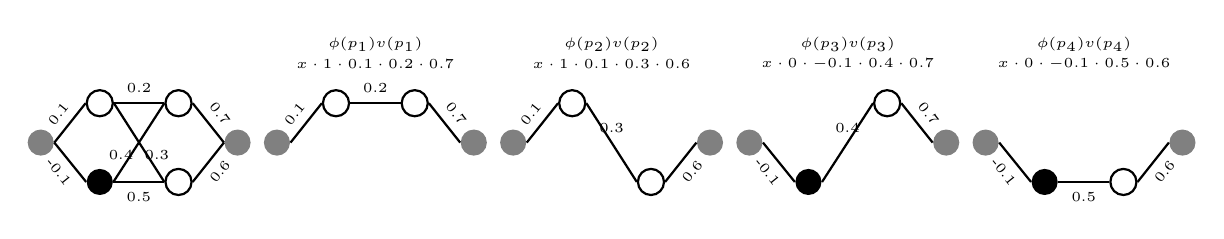
\begin{tikzpicture}
%Top Left
\node[draw,fill=white,circle,thick,
] (tl) at (-0.5,2){};

%Top Right
\node[draw,fill=white,circle,thick,
] (tr) at (0.5,2){};

%Bottom Left
\node[fill=black,circle,
] (bl) at (-0.5,1){};

%Bottom Right
\node[draw,fill=white,circle,thick,
] (br) at (0.5,1){};


%Input
\node[fill=gray,circle,
] (input) at (-1.25,1.5){};


%Output
\node[fill=gray,circle,
] (output) at (1.25,1.5){};

\draw[-, thick] (input.east) -- (tl.west) node [midway, above, sloped] (t1) {\tiny{0.1}};
\draw[-, thick] (input.east) -- (bl.west) node [midway, below, sloped] (t2) {\tiny{-0.1}};
\draw[-, thick] (tl.east) -- (tr.west) node [midway, above, sloped] (t1) {\tiny{0.2}};
\draw[-, thick] (bl.east) -- (br.west) node [midway, below, sloped] (t1) {\tiny{0.5}};
\draw[-, thick] (tl.east) -- (br.west) node [pos=0.85, above] (t1) {\tiny{0.3}};
\draw[-, thick] (bl.east) -- (tr.west) node [pos=0.15, above] (t1) {\tiny{0.4}};
\draw[-, thick] (tr.east) -- (output.west) node [midway, above, sloped] (t1) {\tiny{0.7}};
\draw[-, thick] (br.east) -- (output.west) node [midway, below, sloped] (t1) {\tiny{0.6}};




%%%%%%%%%%%%%%%%%Path 1%%%%%%%%%%%%%%
%Input
\node[fill=gray,circle,
] (p1input) at (1.75,1.5){};


%Output
\node[fill=gray,circle,
] (p1output) at (4.25,1.5){};



%Top Left
\node[draw,fill=white,circle,thick,
] (p1tl) at (2.5,2){};

%Top Right
\node[draw,fill=white,circle,thick,
] (p1tr) at (3.5,2){};




\draw[-, thick] (p1input.east) -- (p1tl.west) node [midway, above, sloped] (t1) {\tiny{0.1}};
\draw[-, thick] (p1tl.east) -- (p1tr.west) node [midway, above, sloped] (t1) {\tiny{0.2}};
\draw[-, thick] (p1tr.east) -- (p1output.west) node [midway, above, sloped] (t1) {\tiny{0.7}};



%%%%%%%%%%%%%%%%%Path 2%%%%%%%%%%%%%%

%Input
\node[fill=gray,circle,
] (p2input) at (4.75,1.5){};


%Output
\node[fill=gray,circle,
] (p2output) at (7.25,1.5){};

%Top Left
\node[draw,fill=white,circle,thick,
] (p2tl) at (5.5,2){};

%Bottom Right
\node[draw,fill=white,circle,thick,
] (p2br) at (6.5,1){};

\draw[-, thick] (p2input.east) -- (p2tl.west) node [midway, above, sloped] (t1) {\tiny{0.1}};
\draw[-, thick] (p2tl.east) -- (p2br.west) node [pos=0.5, above] (t1) {\tiny{0.3}};
\draw[-, thick] (p2br.east) -- (p2output.west) node [midway, below, sloped] (t1) {\tiny{0.6}};



%%%%%%%%%%%%%%%%%Path 3%%%%%%%%%%%%%%

%Input
\node[fill=gray,circle,
] (p3input) at (7.75,1.5){};


%Output
\node[fill=gray,circle,
] (p3output) at (10.25,1.5){};


%Top Right
\node[draw,fill=white,circle,thick,
] (p3tr) at (9.5,2){};

%Bottom Left
\node[fill=black,circle,
] (p3bl) at (8.5,1){};



\draw[-, thick] (p3input.east) -- (p3bl.west) node [midway, below, sloped] (t2) {\tiny{-0.1}};
\draw[-, thick] (p3bl.east) -- (p3tr.west) node [pos=0.5, above] (t1) {\tiny{0.4}};
\draw[-, thick] (p3tr.east) -- (p3output.west) node [midway, above, sloped] (t1) {\tiny{0.7}};


%%%%%%%%%%%%%%%%%Path 4%%%%%%%%%%%%%%

%Input
\node[fill=gray,circle,
] (p4input) at (10.75,1.5){};


%Output
\node[fill=gray,circle,
] (p4output) at (13.25,1.5){};

%Bottom Left
\node[fill=black,circle,
] (p4bl) at (11.5,1){};

%Bottom Right
\node[draw,fill=white,circle,thick,
] (p4br) at (12.5,1){};

\draw[-, thick] (p4input.east) -- (p4bl.west) node [midway, below, sloped] (t2) {\tiny{-0.1}};
\draw[-, thick] (p4bl.east) -- (p4br.west) node [midway, below, sloped] (t1) {\tiny{0.5}};
\draw[-, thick] (p4br.east) -- (p4output.west) node [midway, below, sloped] (t1) {\tiny{0.6}};
%%%%%%%%%%%%%%%%%%%%%%%%%%%%%%

\node[] () at (3,2.75){\tiny{$\phi(p_1)v(p_1)$}};
\node[] () at (3,2.5){\tiny{$x\cdot 1\cdot 0.1 \cdot 0.2 \cdot 0.7$}};

\node[] () at (6,2.75){\tiny{$\phi(p_2)v(p_2)$}};
\node[] () at (6,2.5){\tiny{$x\cdot 1\cdot 0.1 \cdot 0.3 \cdot 0.6$}};

\node[] () at (9,2.75){\tiny{$\phi(p_3)v(p_3)$}};
\node[] () at (9,2.5){\tiny{$x\cdot 0\cdot -0.1 \cdot 0.4 \cdot 0.7$}};

\node[] () at (12,2.75){\tiny{$\phi(p_4)v(p_4)$}};
\node[] () at (12,2.5){\tiny{$x\cdot 0\cdot -0.1 \cdot 0.5 \cdot 0.6$}};




\end{tikzpicture}


}
\caption{Illustration of the dual `path-by-path' view of computations.}
\label{fig:paths}
\end{figure}
\end{comment}
\begin{figure}[!t]
\centering
\begin{minipage}{1.0\columnwidth}
\centering
\begin{minipage}{0.49\columnwidth}
\centering

\resizebox{0.8\columnwidth}{!}{
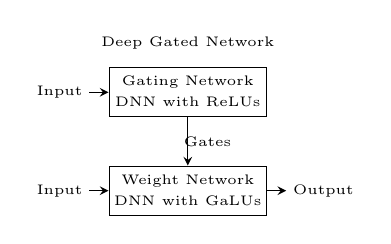
\begin{tikzpicture}

\node []  (fntext)at (5,1) {\tiny{Deep Gated Network}};
%Feature Network
\node [draw,
	minimum width=2cm,
	minimum height=0.625cm,
]  (fnbox)at (5,0.375) {};
\node []  (fntext)at (5,0.5) {\tiny{Gating Network}};

\node []  (fntext)at (5,0.25) {\tiny{DNN with ReLUs}};


%Feature Network Input
\node (fin) [left of=fnbox,node distance=1.25cm, coordinate] {};
\node[left=-1pt] at (fin.west){\tiny{Input}};
\draw[-stealth] (fin.center) -- (fnbox.west);




%Value Network

\node [draw,
	minimum width=2cm,
	minimum height=0.625cm,
]  (vnbox)at (5,-0.875) {};
\node []  (fntext)at (5,-0.75) {\tiny{Weight Network}};
\node []  (vntext)at (5,-1) {\tiny{DNN with GaLUs}};

%Value Network Input
\node (vin) [left of=vnbox,node distance=1.25cm, coordinate] {};
\node[left=-1pt] at (vin.west){\tiny{Input}};
\draw[-stealth] (vin.center) -- (vnbox.west);

%Feature Network Output
\node (vout) [right of=vnbox,node distance=1.25cm, coordinate] {};
\node[right=-1pt] at (vout.west){\tiny{Output}};
\draw[-stealth]  (vnbox.east)--(vout.center);



\draw[-stealth]  (fnbox.south)--(vnbox.north);

\node []  (gates)at (5.25,-0.25) {\tiny{Gates}};


\end{tikzpicture}


}
\end{minipage}
\begin{minipage}{0.49\columnwidth}
\centering

\resizebox{0.8\columnwidth}{!}{
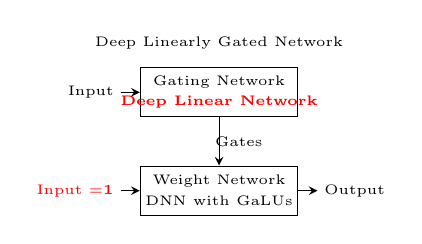
\begin{tikzpicture}

\node []  (fntext)at (5,1) {\tiny{Deep Linearly Gated Network}};
%Feature Network
\node [draw,
	minimum width=2cm,
	minimum height=0.625cm,
]  (fnbox)at (5,0.375) {};
\node []  (fntext)at (5,0.5) {\tiny{Gating Network}};

\node []  (fntext)at (5,0.25) {\tiny{\bf\color{red}{Deep Linear Network}}};


%Feature Network Input
\node (fin) [left of=fnbox,node distance=1.25cm, coordinate] {};
\node[left=-1pt] at (fin.west){\tiny{Input}};
\draw[-stealth] (fin.center) -- (fnbox.west);




%Value Network

\node [draw,
	minimum width=2cm,
	minimum height=0.625cm,
]  (vnbox)at (5,-0.875) {};
\node []  (fntext)at (5,-0.75) {\tiny{Weight Network}};
\node []  (vntext)at (5,-1) {\tiny{DNN with GaLUs}};

%Value Network Input
\node (vin) [left of=vnbox,node distance=1.25cm, coordinate] {};
\node[left=-1pt] at (vin.west){\tiny{\color{red}{Input =$\mathbf{1}$}}};
\draw[-stealth] (vin.center) -- (vnbox.west);

%Feature Network Output
\node (vout) [right of=vnbox,node distance=1.25cm, coordinate] {};
\node[right=-1pt] at (vout.west){\tiny{Output}};
\draw[-stealth]  (vnbox.east)--(vout.center);



\draw[-stealth]  (fnbox.south)--(vnbox.north);

\node []  (gates)at (5.25,-0.25) {\tiny{Gates}};


\end{tikzpicture}


}
\end{minipage}

\end{minipage}
\caption{\small{DGN is a setup to understand the role of gating in DNNs with ReLUs. The DLGN setup completely disentangles and re-arranges the computations in an interpretable manner. The surprising fact that a constant $\mathbf{1}$ input is given to weight network of DLGN is justified by theory and experiments in \Cref{sec:analysis,sec:dlgn}.}}
\label{fig:lgln}
\end{figure}
%{\centering \emph{\textbf{How critical is the entanglement for the success of DNNs? or Can we disentangle? }}\par}

%Note that we are not suggesting that we do away with the non-linearity altogether; we are just asking for the disentanglement. In this paper, we focus on DNNs with rectified linear units (ReLUs). For such DNNs, using the dual view of \cite{npk}, we propose a novel way to disentangle the computations into two linear structures. The `black box'-ness issue is resolved because the two linear structures have simple `mathematical' interpretations.  We also show that entanglement is not critical, i.e., our new proposal achieves results comparable to the state of the art.% on standard dataset and at the same time improves interpretability. 

%In this paper, we focus on DNNs with rectified linear units (ReLUs). For such networks, we argue that the `black box'-ness issue is mostly conceptual one arising from the primal view which is partial and incomplete. The primal view is that, increasingly sophisticated features are learnt in a layer-by-layer manner. The conceptual issue here is that, only the final layer is linear and amenable to a feature/weight interpretation, and yet the hidden features i.e., the penultimate layer outputs are not interpretable themselves. 
%The conceptual issue with the primal view is that, only the final layer is linear and amenable to a feature/weight interpretation, and even then, the hidden features i.e., the penultimate layer outputs, obtained as a result of several non-linear operations on the input are not interpretable themselves. 
%Recently \cite{npk} used the \emph{dual view} to investigate the role of gates (i.e., \emph{on/off} state) of the ReLUs. In this paper, we combine the primal dual views to reduce `black box'-ness issue to that of understanding a two linear structure (one each for primal and dual) and a gating mechanism that is sandwidched between the two.

%The dual view proposes an alternative feature decomposition, by projecting the computation onto the dimnesion of the paths. A path starts from an input node, passes through a weight and a ReLU in each layer and ends at an output node. A path is `active' (i.e., `on') if all the gates in the path are `active' (i.e. `on). Each path, if active, transmits the signal at its input node, which on its way to the output is scaled by a `neural path value' (NPV) which is equal the product of the weights in the path. For a given input, a `neural path feature' (NPF) is defined to be the product of signal at the input node and the path activity. The NPF and NPV are vectors in $\R^{\text{total.no.paths}}$, and the ouput is the inner product of these NPF and NPV. Note that the gates dictate the path activity -- the NPFs are known if the input and the gates are known. So, there is no need for any extra procedure to compute the NPFs. 

%The dual view breaks down the computations path-by-path, and expresses the output as the inner product of a `path feature' and a `path value' (both vectors in $\R^{\text{total\,paths}}$).
%The dual view proposes an alternative feature decomposition, by projecting the computation onto the dimnesion of the paths. 
%A path starts from an input node, passes through a weight and a ReLU in each layer and ends at an output node. 
%A path is `active'  if all the gates in the path are `active' (i.e. `on'). Each path, if active, transmits the signal at its input node, which on its way to the output is scaled by a `path value' which is equal the product of the weights in the path. The `path feature' is the product of signal at the input node and the path activity. %The `path feature' and `path value' are vectors in , and the ouput is the inner product of these two. Note that the gates dictate the path activity -- the `path features' are known if the input and the gates are known. So, there is no need for any extra procedure to compute the `path features'. 


%Before we can talk about the practical use of the NPFs, we need to ask "how good are NPFs as features?", i.e., suppose we have the NPFs in hand, is it possible to learn the NPV and if so how effective will be that model. A trivial answer it that in a DNN with ReLUs the NPF and NPV are learnt simultaenous, so NPFs are indeed good features. However, it is also possible to check in a standalone manner as to whether NPFs are good features. This is achieved by a deep gated network (DGN) setup \citep{npk}, where the gates (i.e., NPFs) are generated by in the feature network, and are used as external masks in a different network called the value network (whose weights specify the NPV) which is responsible for the input to the output computation. It was shown that using the gates (i.e., NPFs) from a pre-trained DNN (by letting it to be the feature network), and training the NPV separately in the value network, one can match the performance of the pre-trained DNN. In short, NPFs are indeed useful features.


%Before we can talk about the practical use of the `path features', we need to ask "how good are these as features?", i.e., suppose we have them in hand, is it possible to learn the `path value' and if so how effective will be that model. A trivial answer it that in a DNN with ReLUs the `path feature' and `path value' are learnt in the same network, so `path features' are indeed good. However, it is also possible to check in a standalone manner the goodness of `path features'. This is achieved by a deep gated network (\texttt{DGN}) setup \citep{npk}, where the gates (i.e., `path features') are generated by in the feature network, and are used as external masks in a different network called the value network (whose weights specify the `path value') which is responsible for the input to the output computation. It was shown that using the gates (i.e., `path features') from a pre-trained DNN (by letting it to be the feature network), and training the `path value' separately in the value network, one can match the performance of the pre-trained DNN. In short, `path features' are indeed good.

%If the path-by-path conceptualisation of the dual view were to be non-vacuous, then any alternative setup that achives this should be good enough. 
%An alternative way to compute path-by-path  is via the deep gated network (DGN) setup \citep{npk}. A DGN has two networks, a feature network which is a DNN with ReLUs, and a value network with gated linear units (GaLUs) \citep{sss}, which need external gating signals. The gates are generated in feature network, and are used as external gating signals to switch `on/off' the GaLUs (and hence the paths) in the value network  which computes the output from input. In other words, the input and the gates of the feature network realises the `path feature', and the value network realises the `path value' and the inner product of the `path feature' and `path value'. %DGN being an alternative to DNN, the following were answered by \cite{npk}.

%The primary use of a DGN was to characterise the information in the gates of a DNN. It was shown that \emph{gates contain the most useful information}: training the value network of a DGN with a pre-trained DNN as its feature network, matches the performance of the pre-trained DNN. It was also shown that \emph{gates are learnt during training} and that it improves test accuracy.


%\textbf{Motivation.} As an alternative model, a DGN performs \emph{only marginally} worse than its corresponding DNN.  By successfully addressing the `black box'-ness issue in a DGN we will have both performance and interpretability. 
%\emph{Is DGN better than DNN?}
%%
%It was shown a DGN train from scratch (i.e., randomised initialisation of both feature and value network) performs \emph{only marginally} worse than DNN. DGN approximated DNN empirically.

%\emph{What is the use of DGN?}

%The primary use of a DGN was to characterise the information in the gates of a DNN. They showed that \emph{gates contain the most useful information}: training the value network of a DGN with pre-trained DNN as its feature network, matches the performance of the pre-trained DNN. It was also shown that \emph{gates are learnt during training} and that it improves test accuracy.

%The secondary use is that a DGN serves as an approximation (to a DNN) which is amenable to theoretical analysis.  %In other words, if we have the `path feature' (via the gates of feature network) then we can train `path value' (in the value network). This implies, in practice, `path feature' is akin to feature and `path value' is akin to weights in a standard linear model, wherein, if the feature is known the weigths can be trained. 


%Using the DGN, \cite{npk} confirmed the non-vacuousness of the dual view by asking (i) \emph{Q1: suppose we have the `path features' in hand, is it possible to learn the %path value' separately?} and (ii) \emph{Q2: can the DGN learn the `path features' and `path value' as good as the DNN}.

%1. \emph{Answer to Q1}.  

%2. \emph{Answer to Q2}. 

% Based on \emph{Answer to Q1}, they concluded that most useful information is in the gates, i.e., the `path features'. They also showed that gates are learnt during training which improves generalisation.
%Before we can talk about the practical use of the `path features', we need to ask "how good are these as features?", i.e., suppose we have them in hand, is it possible to learn the `path value' and if so how effective will be that model. A trivial answer it that in a DNN with ReLUs the `path feature' and `path value' are learnt in the same network, so `path features' are indeed good. However, it is also possible to check in a standalone manner the goodness of `path features'. 
 


 
\begin{comment}
In a DNN with ReLUs, both the `path feature' and `path value' are dictated by the same set of weights. In order to separately understand the roles of the th feature' and `path value', \cite{npk} used a deep gated network setup, wherein, one network computes the gates (i.e., `path features'), the gates are then applied as external masks to turn `on/off' the paths in a different network whose weights specify the `path value' and is resposible for the input to output computation. Using the DGN, \cite{npk} showed the following  results:

1. Gates (i.e., `path features') hold the most useful information. Using the gates of a pre-trained DNN as external masks and training the weights recovers the performance of the pre-trained DNN.

2. Gates (i.e., `path features') are learnt during training of a DNN with ReLUs: gates from a pre-trained DNN perform better than the gates from an randomly initialised DNN.

3. Gates (`path features') and weights ('path values) can be learnt separately.

4. The gates are formally characterised by the so called \emph{neural path kernel} (NPK) which is equal to the \emph{Hadamard} product of the input Gram matrix and a correlation matrix which measures the overlap between the sub-networks of paths active for the various input pairs.
\end{comment}


%We now discuss the deep gated network (DGN) setup which combines the primal and the dual views. In a DNN with ReLUs, both the `path feature' and `path value' are dictated by the same set of weights. On the contrary, in a DGN, there are two networks, a \emph{feature network} which generates the gates, which are then applied as external masks to turn `on/off' the paths in a different network called \emph{value network} whose weights specify the `path value' and is resposible for the input to output computation. In a DGN, the feature network corresponds to the primal view (since the gates are generated in a layer by layer manner) and the value network corresponds to the dual view. Note that by specifing the gates automatically specifies the `path features' as well. DGN setup can be used in two mode. First mode is solely for ablation studies, to separately measure the information in the gates of a pre-trained DNN: fix the feature network to be the pre-trained ReLU and an train only the value network. Secondly mode is an alternative to DNNs with ReLUs: both the feature and value network are trained simultaenous. Using the DGN, \cite{npk} showed the following interesting results:

%The dual view decomposes the computation in a DNN into two parts (i) computation in the gates which is input dependent and (ii) computation in the weights which is the same across inputs. Based on this decomposition, the gates are separated from the weights. The information in the gates is then characterised by keeping the gates fixed, applying them as external masks and then training the weights. In this setting, the following interesting results were shown:

%1. \textbf{ Most information is in the gates}. Using the gates from a pre-trained DNN as external masks one can retrain the weights and match the test accuracy of the original pre-trained DNN with ReLU. 

%2. \textbf{Gate Are Learnt.} It was shown that gates are learnt during training and it improves test accuracy. It was shown that if gates from a randomly initialised (instead of pre-trained) DNN are used as external masks, and the weights are trained, the test accuracy drops significantly. This implies that gates are learnt when a DNN with ReLU is trained.
  
%This implies that most useful input dependent information is in the gates. 

%3. \textbf{Neural Path Kernel For Subnetwork.} For any given input, computation from input to output happens via the `active subnetwork' consisting of active paths.
%It was show that the information stored in the gates is analytically characterised by \emph{neural path kernel} (NPK) which is equal to the \emph{Hadamard} product of the input Gram matrix and a correlation matrix which measures the overlap between the sub-networks active for the input pairs.

%\textbf{Our Contributions.} In the first part of the paper, we look at the issue of `black box'-ness. As mentioned earlier, this issue is conceptual. The main misconception is that \emph{starting from the input each layer performs a non-linear transformation via activations and sophisticated structures are learnt layer-by-layer}. The two things, i.e., `layer-by-layer' and `non-linear activations' are separately correct; the misconception is the need for the two to be entangled. DGN \citep{npk} takes the first step in the disentanglement, by separating the primal and the dual: the feature network computes the gates layer-by-layer (primal) and the value network computes the output path-by-path (dual). We identify two issues with the DGN and rectify it to obtain the novel \texttt{DGN-NO-ACT} which is a white box model. We discuss the issue and our proposals to address them.

%\emph{\textbf{Issue 1:} The feature network which is a DNN with ReLUs is a `black box'.}

%\emph{\textbf{Our Solution:}} We replace the ReLUs with identity activations, and use the pre-activations to trigger the gates, which are then provided to the value network. The transformation from the input to pre-activation has no non-linear activations and interpretable via linear algebraic tools.

%\emph{\textbf{Issue 2}: The value network might be learning sophisticated structures from the input in a layer-by-layer manner, and hence the value network is also a `black box'.}

%\emph{\textbf{Our Solution:}} We give a constant $\mathbf{1}$ as input to the value network, thereby removing any misconception that perhaps sophisticated structures are learnt layer-by-layer in the value network.


%\emph{\textbf{Issue 3:} Are we not impeding the layer-by-layer learning ability by providing a $\mathbf{1}$ input?}

%\emph{\textbf{Our Answer:}} No. All the layer-by-layer learning from input happens in the feature network (without use of non-linear activations), so we are not doing way with this aspect.


%\textbf{Our Contributions.} In the first part of the paper, we look at the issue of `black box'-ness. As mentioned earlier, this issue is conceptual. The main misconception is that \emph{starting from the input each layer performs a non-linear transformation via activations and sophisticated structures are learnt layer-by-layer}. The two things, i.e., `layer-by-layer' and `non-linear activations' are separately correct; the misconception is in the need for these two to be entangled. DGN \citep{npk} takes the first step in the disentanglement, by separating the primal and the dual: the feature network computes the gates layer-by-layer (primal) and the value network computes the output path-by-path (dual). We propose a novel white box model \texttt{DGN-NO-ACT} by modifying the DGN. The hightlights are:


\textbf{Our Contribution.}  The NTK theory provides a kernel interpretation of DNNs. The dual view provides a `learning in the gates + learning in the weights given gates' interpretation, in which, the learning in the weights is linear in the path space and has a kernel interpretation via the NPK. In this paper, we extend the dual view with a focus on `black box'-ness. Our contributions are listed below.


$\bullet$\textbf{Extending Dual View}(\Cref{sec:analysis}).  We present an unnoticed insight in prior work on fully connected networks that the \textbf{NPK is a product kernel} and is invariant to layer permutations. We extend the dual view to show that the NPK is rotationally invariant in the presence of convolutions with global average pooling, and NPK is an ensemble of many kernels in the presence of skip connections. 

$\bullet$ \textbf{Disentangling Using Dual View}(\Cref{sec:dlgn}). To address the issue of `black box'-ness, we disentangle the `gating network' as well as `weight network'. For this purpose, we propose a a novel Deep \emph{Linearly} Gated Network (DLGN) as a \emph{mathematically interpretable} counterpart of a DNN with ReLUs (see \Cref{fig:lgln}).  In a DLGN, the gating network is a deep linear network, i.e., there are no non-linear activations. Thus, the transformation from input to the pre-activations are linear matrix operations; this \emph{disentangles the gating network}. We then argue via theory and experiments that the  \emph{weight network is disentangled in the path space}. For this, we experimentally show that, destroying the layer-by-layer structure by permuting the gates and providing a constant $\mathbf{1}$ as input (see DLGN in \Cref{fig:lgln}) do not  degrade performance. These counter intuitive and surprising results are difficult to reconcile using the commonly held `sophisticated structures are learnt layer-by-layer' interpretation. However, these experimental results follow from theoretical results and insights in \Cref{sec:analysis}.  In other words, the right approach is to think that learning in the weight network happens path-by-path, which is interpreted via the NPK. Using the fact that NPK is solely based on input and the gates, and the fact that, in a DLGN, the pre-activation to the gates are linearly functions of the input, we have complete disentanglement and interpretability.
%(ii) use the dual view to address the problem of `black-box'ness. The contributions are listed below.

%$\bullet$ \textbf{Extending Dual View.} In \Cref{sec:analysis}, we first revisit the NPK expression in \citep{npk}. A previously unnoticed property of the NPK is that it is invariant to layer permutation. In \Cref{th:fc}, we explicitise this invariance by rewriting the NPK as a \emph{Hadamard} product of the input Gram matrix and the base kernels (one per layer) which measures the average \textbf{correlation of gates} (in those layers). In \Cref{th:conv,th:res}, we extend the dual view to show that the NPK is rotationally invariant in the presence of convolutions with global average pooling, and NPK is an ensemble of many kernels in the presence of skip connections respectively.  %The most important take away is that the \emph{correlation of gates} is key.


%$\bullet$ \textbf{Disentangling Using Dual View.} While the DGN disentangles the computations in the gates from those in the weights, there are two issues related to `black box'-ness: (i) the `gating network' itself is a DNN with ReLUs, and (ii) the `weight network' has GaLUs and the linear operations entangled and is perhaps learning sophisticated structures in its hidden layers. To address these issues, first, we modify the DGN  to propose a novel Deep \emph{Linearly} Gated Network (DLGN) as a \emph{mathematically interpretable} counterpart of a DNN with ReLUs (see \Cref{fig:lgln}).  In a DLGN, the gating network is a deep linear network, i.e., there are no non-linear activations. Thus, the transformation from input to the pre-activations are linear matrix operations; this \emph{disentangles the gating network}. Second, even though the GaLUs and the linear operations are entangled in each layer, we show that `layer-by-layer' interpretation itself is not meaningful, and hence we need not worry about the entanglement in the layers, especially, in relation to interpertability. In \Cref{sec:dlgn}, we experimentally show that, destroying the layer-by-layer structure by permuting the gates and providing a constant $\mathbf{1}$ as input (see DLGN in \Cref{fig:lgln}) do not  degrade performance. These counter intuitive and surprising results are difficult to reconcile using the commonly held `sophisticated structures are learnt layer-by-layer' interpretation.  Yet, these results follow from \Cref{th:fc}, which shows correlation of the gates is the key: while permuting the gates/providing a constant $\mathbf{1}$ as input the correlation of the gates is not lost. In other words, the \emph{disentanglement  happens in the path space}, i.e., the right approach is to think that learning in the weight network happens path-by-path, which is interpreted via the NPK. Using the fact that NPK is based on input and the gates alone, and the fact that, in a DLGN, the pre-activation to the gates are linearly functions of the input, we have complete disentanglement and interpretability.


% In \Cref{sec:dlgn}, using the dual view, we disentangle both `gating network'  as well as  `weight network', and in doing so, our aim is to ask `\textbf{how critical is entanglement for the success of DNNs with ReLUs?}'. For this purpose,
%$\bullet$ \textbf{Disentangling Using Dual View.} In \Cref{sec:dlgn}, using the dual view, we disentangle both `gating network'  as well as  `weight network', and in doing so, our aim is to ask `\textbf{how critical is entanglement for the success of DNNs with ReLUs?}'. For this purpose, we modify the DGN  to propose a novel Deep \emph{Linearly} Gated Network (DLGN) as a \emph{mathematically interpretable} counterpart of a DNN with ReLUs (see \Cref{fig:lgln}).  In a DLGN, the gating network is a deep linear network, i.e., there are no non-linear activations. Thus, the transformation from input to the pre-activations are linear matrix operations; this \emph{disentangles the gating network}. Even though the GaLUs and the linear operations are entangled, we argue that \emph{disentanglement of weight network} happens in the path space, and the layer-by-layer view can be safely ignored. In \Cref{sec:dlgn}, we experimentally show that, destroying the layer-by-layer structure by permuting the gates and providing a constant $\mathbf{1}$ as input (see DLGN in \Cref{fig:lgln}) do not  degrade performance. These counter intuitive and surprising results are difficult to reconcile using the commonly held `sophisticated structures are learnt layer-by-layer' interpretation.  Yet, these results follow from \Cref{th:fc}, which shows correlation of the gates is the key: while permuting the gates/providing a constant $\mathbf{1}$ as input the correlation of the gates is not lost.

\textbf{Message.} The DLGN is not an alternative architecture per se, but a disentanglement and an interpretable re-arrangement of the computations in a DNN with ReLUs. The DLGN disentangles the computations into two  `mathematically' interpretable linearities (i) the `primal' linearity between the input and the pre-activations, and (ii) the `dual' linearity in the path space, and the role of gating is to \emph{lift} the primal to the dual. Dual linearity is characterised by the NPK which is based on input and gates. We compare the performance of DNN, DGN and DLGN on CIFAR-10 and CIFAR-100 to show that, the DLGN recovers more than $86\%$ of the performance of the DNN, which implies that while entanglement in the DNNs enable their improved performance,  the `disentangled and interpretable'  computations in the DLGN can still recover most part of the performance.

%The NTK theory provides a `kernel' interpretation of DNNs. The dual view provides a `learning in gates + learning in weights given gates (NPK)'  interpretation. 
%By such disentanglement, we show that the commonly view of sophisticated structures being learnt in a layer-by-layer manner is a misconception. 

%Here, `Gated-Linear' is due to the use of GaLUs  and `Linearly' is because the pre-activation to the gates are derived linearly from the input. LGLN helps in disentangling by addressing the following open questions.

%{\centering \emph{\textbf{Do we need non-linearity to learn the right way to trigger the gates?}}\par}

%Thus, the learning of structures in a `layer-by-layer manner' is linear and not sophisticated.

%{\centering \emph{\textbf{How to interpret the learning of weights given the external gates?}}\par}
%In a LGLN, once the gates are triggered the computations are handed over to the part of the network consisting of GaLUs. 



%The constant $\mathbf{1}$ input to the bottom network of LGLN while counter intuitive and surprising, is at the same time easily justified by dual linearity: the neural path value is a vector specifying the contribution of each path to the final output and the neural path feature is a vector specifying which path to be selected and which one to be left out.  In \Cref{sec:exp}, we experimentally show that, providing a constant $\mathbf{1}$ as input and destroying the layer-by-layer structure by permuting the gates  do not cause a degradation in performance



%which has an interpretation in terms of the NPK. To drive home our point we first revisit the NPK expression in \citep{npk}. A previously unnoticed property of the NPK is that it is invariant to layer permutation. In \Cref{th:fc}, we explicitise this invariance by rewriting the NPK as a \emph{Hadamard} product of the input Gram matrix and the base kernels (one per layer) which measures the average correlation of gates (in those layers). In \Cref{sec:exp}, we experimentally show that, destroying the layer-by-layer structure by permuting the gates and providing a constant $\mathbf{1}$ as input do not cause a degradation in performance. These are counter intuitive and surprising results that are difficult to reconcile using the commonly held `sophisticated structures are learnt layer-by-layer' interpretation.  However, looked via the NPK expression, it is easy to understand why the constant $\mathbf{1}$ input does not hurt: because it only makes the input Gram matrix a constant, and the NPK still has the product of base kernels that encode the input dependent information. Further, the permutation invariance of the NPK implies that destroying the layer-by-layer structure does not hurt. In other words, once the gates are known, it is enough to understand path-by-path view, and the layer-by-layer view can be ignored.

%Thus we disentangle the computations into two  `mathematically' interpretable linearities (i) the `primal' linearity between the input and the pre-activations, and (ii) the `dual' linearity in the path space, and the role of gating is to \emph{lift} the primal to the dual. Dual linearity is characterised by the NPK which has a product of base kernels structure wherein the base kernels correspond to the gating features.  We show that LGNLs of standard DNNs achieve greater than $90\%$ on CIFAR-10 and close to $70\%$ accuracy on CIFAR-100. 

%\textbf{Remark:} LGLN is not an alternative architecture per se, but a disentanglement and an interpretable re-arrangement of the computations in a DNN with ReLUs.

%as a possible reason for success, and show that once the gates are triggered the path-by-path view is the right way to interpret.


% i.e., if we look at the output as the inner product of neural path feature and neural path value. In a LGLN, the neural path value is a vector specifying the contribution of each path to the final output and since the input is $\mathbf{1}$, the neural path feature is a $0/1$ vector specifying which path to be selected and which one to be left out. We call this \textbf{dual linearity}, i.e., linearity in the `path' variables. 
 
% We revisit the \emph{external-fixed gates setting} in \citep{npk}. A previously unnoticed property of the NPK is that it is invariant to layer permutation. In \Cref{th:fc}, we explicitise this invariance by rewriting the NPK as a \emph{Hadamard} product of the input Gram matrix and the base kernels (one per layer) which measures the average correlation of gates (in those layers).  The constant $\mathbf{1}$ input is thus justified: here only the input Gram matrix is a constant, and the \emph{Hadamard} product of the the base kernels still posses useful information.  In \Cref{th:conv,th:res}, we extend the dual view to show that the NPK is rotationally invariant in the presence of convolutions with global pooling, and NPK is an ensemble of many kernels in the presence of skip connections respectively.  

%Note that the very fact that computations happen path-by-path is why we are able to present a constant $\mathbf{1}$ input to the bottom network of LGLN. 






%$\bullet$ \textbf{Disentangling Feature Network.} In the feature network of \texttt{DGN-NO-ACT}, we replace the ReLU activations by identity activations. Thus, the computations in the feature network are not entangled with non-linearities. Since the feature network is entirely linear, we do not need additional `local linearised' interpretation. We call the linearity of feature network as \textbf{primal linearity}.

%$\bullet$ \textbf{Disentangling Value Network.} While there is entanglement of GaLUs and the linear operations,  the value network computes path-by-path and not layer-by-layer: the value network is \textbf{dual linear}. Thus, the disentanglement happens in the path variables. While finite width value network is dual linear in the `path' variables, it is not linear in the network weights. However,  dual linearity has a kernel interpretation in the \emph{infinite width regime}  (see discussion on dual linearity below).

%$\bullet$ In essence, the \texttt{DGN-NO-ACT} disentangles the computations into : (i) the `primal linear' feature network which is interpretable in itself, (ii) the `dual linear' value network which has a kernel interpretation, and (iii) the gating non-linearities that serve the purpose of \emph{lifting} the computations from  primal to dual. 
%Note: The dual linearity of value networks holds true for both DGN as well as \texttt{DGN-NO-ACT}.

%we propose a novel (\Cref{sec:dgn-no-act}) in which the ReLU activations in the feature network are replaced by identity activations, and the gates are triggered by the pre-activations from the feature network.  The value network of \texttt{DGN-NO-ACT} remains unchanged (i.e., is same as DGN). We show that \texttt{DGN-NO-ACT}s based on VGG and a ResNet model achieve greater than $90\%$ and close to $70\%$ accuracy on CIFAR-10 and CIFAR-100 respectively (see \Cref{sec:dgn-no-act-cifar}). Using the \texttt{DGN-NO-ACT} we present two main messages:


%$\bullet$ \textbf{Message 1:} The computations in the feature network are linear and do not need additional `local linearisation' for the sake of interpretation.  We call this \emph{primal linearity}. 

%$\bullet$ \textbf{Message 2:}  In a DGN, as well as in the \texttt{DGN-NO-ACT} there is no entanglement in the value network. In other words, the  i.e., . This leads to a kernel interpretation in the \emph{infinite width regime}.


%In a DGN, the primal layer-by-layer comptutation happens in the feature network. However, the issue is that the feature network is a DNN in which the linear matrix multiplication and non-linear activations are entangled. In our novel \texttt{DGN-NO-ACT}, we disentangle by replacing the ReLU activations in the feature network by identity activations thereby making the feature network `primal linear'. The gates are then activated by the pre-activations.  The value network \texttt{DGN-NO-ACT} is same as the one in DGN. The value network is linear in the `path' variables and yet, it is non-linear in the network weight. However, a kernel interpretation is obtained in the \emph{infinite width regime}. 
%The main conceptual roadblock occurs because each layer entangles linear matrix multiplication and non-linear activations. In our novel \texttt{DGN-NO-ACT} (\Cref{sec:dgn-no-act}), we modify the DGN to achieve complete disentanglement. Specifically, we modify the feature network by replacing its ReLU activations by identity activations; this makes it primal linear. In a DGN, the value network is already dual linear, i.e, linear in the `path' variables. The key points are:

%$\bullet$ \textbf{Primal Linearity:} We replace the ReLUs in the feature network with identity activations. This makes the feature network free of activations and entirely linearly.  

%$\bullet$ \textbf{Gating:} The preactivations from the feature network are used to trigger the gates. The gates here are seen to play the role of handing off the computations from the primal to the dual.

%$\bullet$ \textbf{Dual Linearity:} We set the input to the value network, so that the `path value' has no input dependence. The value network can be described in simpled terms as:

%{\centering \emph{\textbf{The output is the summation of `path value' weighted by the `path activations'.}}\par}


%$\bullet$ In a \texttt{DGN-NO-ACT}, we defer a formal analysis of how the feature network learns useful gating patterns to future work. Instead, in \Cref{sec:primal}, we informally argue via standard linear algebra that the feature network might be looking at all possible spectral components of the input.

%$\bullet$ Understading Primal Linearity in a \texttt{DGN-NO-ACT}

%The transformation from the input to the pre-activation is linear, which in turn activate the gates. We defer a formal analysis of how the feature network learns useful pre-activations to future work. However, the linearity of feature network is itself a huge gain, because, we do not have to resort to `locally linear explainations' using other models.

%$\bullet$ Understading Dual Linearity in DGN and \texttt{DGN-NO-ACT}

%$\bullet$ \textbf{Dual Linearity (Theory).} We extend the dual view to cover convolutions with global pooling and skip connections.

%Prior work by \cite{ntk,arora2019exact,cao2019generalization} showed that training an infinite width DNN is equivalent to a kernel method with the so called \emph{neural tangent kernel} (NTK). \citep{npk} showed that in an infinite width fully connected DGN with its gates fixed, the NTK is equal (up to a scalar) to the so called \emph{neural path kernel} (NPK) (equal to the Gram matrix of the `path features'). An important property of the NPK which was unnoticed is that the NPK is invaraint to permutation of layers. In \Cref{th:fc}, we explicitise this invariance by rewriting the NPK as a \emph{Hadamard} product of the input Gram matrix and the base kernels (one per layer) which measures the average correlation of gates (in those layers). The expression also reveals that the role of depth is to provide the product structure and the role of width is averaging. %Thus, thanks to the primal dual separation, \Cref{th:fc} captures the roles of gates, depth and width in a single NPK expression. 
%In \Cref{th:conv,th:res}, we extend the dual view to show that the NPK is rotationally invariant in the presence of convolutions with global pooling, and NPK is an ensemble in the presence of skip connections respectively. 

%$\bullet$ \textbf{Dual Linearity (Experiments).}  In \Cref{sec:exp}, we show that the value network does not learn in a layer-by-layer manner, instead learns path-by-path.
%here are two sources via which the input affects the value network, and we destroy both of them. Firstly, we provide the value network with a constant $\mathbf{1}$, ensuring that the only way input dependent information affects the value networks is via the other source namely the gates. 
%We destroy the layer-by-layer structure by permuting the gates and also provide a constant $\mathbf{1}$ as input. We show that these does not cause a degradation in performance: counter intuitive and surprising from the primal view. However, results in \Cref{th:fc,th:conv,th:res} easily explains these.%the dual view easily explains these. %From the expression of \Cref{th:fc}, we know that the input Gram matrix will be a constant. However, the product of the base kernels still contain information about the input. Also, the permutation invariance of the product structure of the NPK allows us to destroy the layer-by-layer structure of the gates.



%$\bullet$ In our novel \texttt{DGN-NO-ACT}, we achieve complete disentanglement of feature network, gating and value network. In the feature network, we replace the ReLUs with identity activations, and use the pre-activations to trigger the gates which are now external to the feature network. The gates are then provided to the value network. We give a constant $\mathbf{1}$ as input to the value network, and hence the `path value' is a vector inin $\R^\text{{total\,paths}}$ and contains no input dependent information. The `path feature' is a vector in $[0,1]^\text{{total\,paths}}$ which specifies the activation levels of each path. In simple terms,

%More importantly, the path activations are dictated by the gates, and transformation from the input to  pre-activation of the gates has no non-linear activations and interpretable via linear algebraic tools.

%$\bullet$ We show that \texttt{DGN-NO-ACT}s corresponding to VGG and a ResNet model achieve greater than $90\%$ and close to $70\%$ accuracy on CIFAR-10 and CIFAR-100 respectively. 

%While prior results \cite{} have also noted the ensemble nature, we believe \Cref{th:res} is more fundamental due to the fact that it is simply based on the presence of combinatorially many architectures caused as a direct consequnce of the skip connections. 

%$\bullet$ In \Cref{sec:theory}, we also revisit prior result for the full connected case. 


%\textbf{Simplifed Interpretation.} As we said, the main misconception is entangling the `layer-by-layer' and the non-linear activations. What we achieve is disentanglement: in our novel \texttt{DGN-NO-ACT} the feature network learns layer-by-layer, and the value network learns path-by-path, and the non-linerity, i.e., gating uses pre-activation from feature network and switches the paths `on/off' in the value network. The proposed \texttt{DGN-NO-ACT} has the following simple interpretation: `path value' is a vector in $\R^\text{{total\,paths}}$ and the `path feature' is a vector in $[0,1]^\text{{total\,paths}}$ which specifies the activation levels of each coordinate in `path value to produce the final output.


%\textbf{Prior Work.} The path-by-path dual view gives subnetwork interpretation. For each input, only a subset of gates are active, and correspondingly only a subnetwork of the paths are active (the `path feature' of the inactive paths is $0$). The Gram matrix of the `path features' is the so called the \emph{neural path kernel} (NPK) and is equal to the \emph{Hadamard} product of input Gram matrix and a correlation matrix which measures the overlap between the active subnetworks active for the various input pairs. \cite{npk} also showed that training the infinite width DGN (with gates fixed) is equivalent to a kernel method with the NPK.

%\textbf{Contribution I.} An important property of the NPK which was unnoticed is that the NPK is invaraint to permutation of layers. In \Cref{th:fc}, we remedy this by rewriting the NPK as a \emph{Hadamard} product of the input Gram matrix and the base kernels (one per layer) which measures the average correlation of gates (in that layer). In \Cref{th:conv} we show that the role of convolutions with global pooling is to provide rotational invariance to the NPK. In \Cref{th:res} we show that the role of skip connections is to provide an ensemble structure to NPK. 

%\textbf{Contribution II.} Once we have the gates from feature network, we show that destroying the layer-by-layer structure by permuting the layers before applying to the value network does not degrade the performance. It could be argued that the value network still manages to recover in a layer-by-layer manner despite such layer permutations. In order to eliminate this argument, we provide a constant $\mathbf{1}$ input to the value network, and observe that even this does not degrade performance. From the primal viewpoint, these are surprising and counter intuitive results. However, in the dual view these are readily reconciled. We know from \Cref{th:fc}, that a constant $\mathbf{1}$ input to the value network sets the input Gram matrix to be a constant, and the NPK is then simply the product of base kernels, which is invariant to layer permutations. In short, the value network indeed computes path-by-path.

%i.e., each path starts with $1$ at its input nodes, only the path activity is input dependent (since it is directly controlled by the gates). Using a constant $\mathbf{1}$ input does not degrade the performance either. 


%\emph{\textbf{Issue 2:} The feature network which is a DNN with ReLUs is a `black box'.}

%\textbf{Contribution III.}  We call this modified DGN as \texttt{DGN-NO-ACT}, and 
%\textbf{White Box.} The \texttt{DGN-NO-ACT} is entirely intrepretable and white box. The feature network generates the pre-activations to the gates without use of non-linear activations, the gates then switch the paths `on/off' to realise the `path features' in the value network which the just computes the inner product between the `path feature' and `path value'.

%In this paper, we improve and simplilfy the DGN to build an entirely interpretable white box DNN. The DGN serves as a good starting point,  in that, it combines the primal view: feature network generating the gates (i.e, `path features') in a layer by layer manner, and the dual view: the value network specifying the `path values' and computing the output (i.e., inner product). We remove the `black box'ness by (i) interpreting the  `path features', (ii) interpreting the  `path value' and (iii) removing non-linear activations in the feature network. 



% This permutation invariance was unnoticed in prior work, and is a key property of the gating features that has surprising and counter intuitive implications (see Q7 and A7 below). In \Cref{th:fc}, we essentially rewrite the prior NPK expression in a way that explicitly reveals this permutation invariance. The main highlight is that each layer is associated with a base kernel which measures the average correlation of gates, and the NPK is a \emph{Hadamard} product of the input Gram matrix and the base kernels. Here, the role of width is averaging and the role of depth is endowing the product structure from which the permutation invaraince ensues. In \Cref{th:conv} we show that the role of convolutions with global pooling is to provide rotational invariance to the NPK. In \Cref{th:res} we show that the role of skip connections is to provide an ensemble structure to NPK. 


%\textbf{Interpreting `Path Value'.}  As per the dual view, all that is there to the value network is `path value', \emph{can we rule out the possibility that the value network is learning sophisticated structures in a layer by layer manner?}. Since `path value' is akin to a weight vector it is interpretable in a straightforward manner, which means we only have the feature network to interpret.

%\textbf{Contribution II.} In the second part of the paper (see \Cref{sec:randlabel}), we look at the following open question in \citep{randlabel}: \emph{when trained upstream with random labels followed by downstream training with true labels, the test accuracy degrades, why?} We show that the degradation in the test performance is because the gates. We also show that in the \emph{external-fixed gates} setting, using the gates from a pre-trained DNN and then training the weights first upstream with random labels followed by downstream training of true labels does not cause significant degradation in test accuracy. These results point out to the importance of the gating.

%Using the dual view, we interpret the roles of (i) width, (ii) depth, (iii) convolutions with global pooling and (iv) skip connections. For this, we refine and extend prior work to derive new results on the structure of NPK. We then present two new empirical results that are easily reconciled in the dual view (as opposed to the primal). These results are not meant to be techniques/tricks to improve performance that `beats state of the art'. The significance is that they showcase the power of dual view in resolving novel and unseen scenarios. We now list these contributions section-wise.

%$\bullet$ In \Cref{sec:theory}, we refine prior result on NPK (which depended on the correlation subnetworks) to show that NPK depends on the \emph{correlation of gates}. The main highlight is that each layer is associated with a base kernel which measures the average correlation of gates, and the NPK is a \emph{Hadamard} product of the input Gram matrix and the base kernels. This implies that the role of width is averaging and the role of depth is to form a product kernel. In \Cref{th:conv} we show that the role of convolutions with global pooling is to provide rotational invariance to the NPK. In \Cref{th:res} we show that the role of skip connections is to provide an ensemble structure to NPK.


%$\bullet$ In \Cref{sec:permute}, we present surprising results that are counter intuitive with respect to the primal view that progressively sophisticated structures are being in a layer by layer manner. Firstly, we show that destroying the layer by layer structure by permuting the gates does not cause performance to degrade at all. Secondly, we show that once the gates are obtained from the input, the network can be provided with a constant $\mathbf{1}$ input without degrading performance. We argue that these counter intuitive results are easily reconciled in the dual view.

%\emph{Part II: Open question related to training with random labels.}

% In \Cref{sec:randlabel}, we show that upstream training with random labels followed by downstream training with true labels degrades test accuracy because the random labels affects the gates. This degradation of test accuracy was an open question in \cite{randlabel}.


%\emph{Part III: Entirely interpretable and white box model.}

%In \Cref{sec:whitebox}, we propose a novel model by modifying  DNNs with ReLUs: we generate the pre-activation to the gates without any non-linear activations. Interpreted in the dual view, this novel model is entirely white box. We show white box models obtained by modifying VGG and a ResNet (in the proposed way) achieve greater than $90\%$ and close to $70\%$ on CIFAR-10 and CIFAR-100 respectively. 


%we propose a novel architecutre obtained by modifying DNNs with ReLUs, which, is conceptually same as DNNs with ReLUs but is entirely interpretable and white box. We effect the modification on a stardard model namely VGG and a ResNet model, to derive the corresponding white box models. We show these white box models achieve greater than $90\%$ and close to $70\%$ on CIFAR-10 and CIFAR-100 respectively. Here, the aim is to demonstrate that the new white box models improve interpretablity without significant loss in performance with respect to `state of the art'.


%We follow up this claim by completely removing the `black box'-n ess: we propose a novel architecutre, which, is conceptually same as DNNs with ReLUs but is entirely interpretable and white box. 
\begin{comment}
\subsection{Dual View}
In the dual view, the computation in a DNN is broken down into paths, wherein, each path starts from the input node, passes through a weight and a ReLU in each layer and ends at the output node. This gives a subnetwork intepretation: for any given input, computation from input to output happens via the `active subnetwork' consisting of active paths. This active subnetwork is in turn formed by the active gates in each layer. Each gate is a just a  simple `perceptron' which is described by the hyperplane of its incoming weights. As the the input passes through the layers, gates are turned on/off based on the angle between the layer input and the hyperplanes associated with the various gates in that layer. 


 The separation is achieved by a \emph{deep gated network} (DGN) setup, wherein, the input dependent gates are generated in a so called \emph{feature network} (which a DNN with ReLU whose sole  is  generation of the gates) and then gating signals are applied as external masks to a so called \emph{value network} which carries out the input to output computation. Having separated the gates and the weights, the role of gates and active subnetworks was investigated in theory and experiments.

%The main result  It was shown that most useful information is in the gates.  

%The dual view (i) gives simpler feature/value decomposition, (ii) gives a subnetwork intepretation and (iii) allows to separate the gates from the weights. We briefly described these below.

%Each path has a signal at its input node, which is gets transmitted to the output if the path is on (i.e., all the gates in the paths are on). On its way to the output, (if path is active) the input signal of a path is scaled by a `value' equal the product of the weights in the path. The input and the on/off of the path is encoded in a so called  and the scaling by the weights is encoded by the \emph{neural path value} (NPV $\in \R^{\text{total-paths}}$). This conceptual separation of computation in the gates encoded in the NPF and the computation in the weights in the NPV has the following favourable points:

%$\bullet$ \textbf{Simplicity.} The input and the gates of a path are  encoded in a \emph{neural path feature} (NPF $\in \R^{\text{total-paths}}$). The weights are encoded in a \emph{neural path value} (NPV $\in \R^{\text{total-paths}}$). The NPF coordinate of a path is $0$ if the path is inactive and is equal to the signal at the input node if the path is active.  The NPV coordinate of a path is the product of the weights in the path. The NPV of a path the scales signal at it input node, and the final DNN output is the inner product of NPF and NPV.

%$\bullet$ \textbf{Interpretability.} For any given input, computation from input to output happens via the `active subnetwork' consisting of active paths. This active subnetwork is in turn formed by the active gates in each layer. Each gate is a `perceptron' which is described by the hyperplane of its incoming weights. As the the input passes through the layers, gates are turned on/off based on the angle between the layer input and the hyperplanes associated with the various gates in that layer. 

%$\bullet$ \textbf{Separation.} 
%In a DNN with ReLUs, the weights play a dual role: (i) they decide the on/off activity of the gates, i.e., the NPF and they also dictate the NPV. 
%To understand the role of gates and weights separately, the gates are also physically separated from the weights in \emph{deep gated network} (DGN) setup, wherein, the input dependent gates are generated in a so called \emph{feature network} (which a DNN with ReLU whose sole  is  generation of the gates) and then gating signals are applied as external masks to a so called \emph{value network} which carries out the input to output computation. Having separated the gates and the weights, the role of gates and active subnetworks was investigated in theory and experiments.

1. \textbf{Gate Learning.} Most information is stored in the gates. Using the gates from a pre-trained DNN as external masks one can retrain the weights of the value network and match the test accuracy of the original pre-trained DNN with ReLU. It was shown that gates are learnt during training and it improves test accuracy.  
%This implies that most useful input dependent information is in the gates. 
%It was shown that if gates from a randomly initialised (instead of pre-trained) DNN are used as external masks, and the weights are trained, the test accuracy drops significantly. 
%This implies that gates are learnt when a DNN with ReLU is trained and

2. \textbf{Neural Path Kernel.} The information stored in the gates is analytically characterised by \emph{neural path kernel} (NPK) which is equal to the \emph{Hadamard} 
\end{comment}
\begin{comment}

\subsection{Dual View}
In the dual view, the computation in a DNN is broken down into paths, wherein, each path starts from the input node, passes through a weight and a ReLU in each layer and ends at the output node. This gives a subnetwork intepretation

 and allows to separate information in the gates from the weights. The main result  It was shown that most useful information is in the gates.  

%The dual view (i) gives simpler feature/value decomposition, (ii) gives a subnetwork intepretation and (iii) allows to separate the gates from the weights. We briefly described these below.

%Each path has a signal at its input node, which is gets transmitted to the output if the path is on (i.e., all the gates in the paths are on). On its way to the output, (if path is active) the input signal of a path is scaled by a `value' equal the product of the weights in the path. The input and the on/off of the path is encoded in a so called  and the scaling by the weights is encoded by the \emph{neural path value} (NPV $\in \R^{\text{total-paths}}$). This conceptual separation of computation in the gates encoded in the NPF and the computation in the weights in the NPV has the following favourable points:

%$\bullet$ \textbf{Simplicity.} The input and the gates of a path are  encoded in a \emph{neural path feature} (NPF $\in \R^{\text{total-paths}}$). The weights are encoded in a \emph{neural path value} (NPV $\in \R^{\text{total-paths}}$). The NPF coordinate of a path is $0$ if the path is inactive and is equal to the signal at the input node if the path is active.  The NPV coordinate of a path is the product of the weights in the path. The NPV of a path the scales signal at it input node, and the final DNN output is the inner product of NPF and NPV.

$\bullet$ \textbf{Interpretability.} For any given input, computation from input to output happens via the `active subnetwork' consisting of active paths. This active subnetwork is in turn formed by the active gates in each layer. Each gate is a `perceptron' which is described by the hyperplane of its incoming weights. As the the input passes through the layers, gates are turned on/off based on the angle between the layer input and the hyperplanes associated with the various gates in that layer. 

$\bullet$ \textbf{Separation.} 
%In a DNN with ReLUs, the weights play a dual role: (i) they decide the on/off activity of the gates, i.e., the NPF and they also dictate the NPV. 
To understand the role of gates and weights separately, the gates are also physically separated from the weights in \emph{deep gated network} (DGN) setup, wherein, the input dependent gates are generated in a so called \emph{feature network} (which a DNN with ReLU whose sole  is  generation of the gates) and then gating signals are applied as external masks to a so called \emph{value network} which carries out the input to output computation. Having separated the gates and the weights, the role of gates and active subnetworks was investigated in theory and experiments.

\textbf{Key Results.}  

1. \textbf{Gate Learning.} Most information is stored in the gates. Using the gates from a pre-trained DNN as external masks one can retrain the weights of the value network and match the test accuracy of the original pre-trained DNN with ReLU. It was shown that gates are learnt during training and it improves test accuracy.  
%This implies that most useful input dependent information is in the gates. 
%It was shown that if gates from a randomly initialised (instead of pre-trained) DNN are used as external masks, and the weights are trained, the test accuracy drops significantly. 
%This implies that gates are learnt when a DNN with ReLU is trained and

2. \textbf{Neural Path Kernel.} The information stored in the gates is analytically characterised by \emph{neural path kernel} (NPK) which is equal to the \emph{Hadamard} product of the input Gram matrix and a correlation matrix which measures the overlap between the sub-networks active for the input pairs.
\end{comment}
\begin{comment}

\textbf{Neural Path Feature.} In the dual view, the computation in a DNN is broken down into paths, which leads to an alternative feature/value decomposition. Each path has a signal at its input node, which is gets transmitted to the output if the path is on (i.e., all the gates in the paths are on). On its way to the output, (if transmitted) the input signal of a path is scaled by a `value' equal the product of the weights in the path. The input and the on/off of the path is encoded in a so called \emph{neural path feature} (NPF $\in \R^{\text{total-paths}}$) and the scaling by the weights is encoded by the \emph{neural path value} (NPV $\in \R^{\text{total-paths}}$). The DNN output for an input $x\in\R^{\din}$ , and parameter $\Theta\in\R^{\dnet}$ is given by:
\begin{align}
\texttt{DNN-OUTPUT(x)=}\ip{\texttt{NPF}_{\Theta}\texttt{(x),NPV}_{\Theta}}
\end{align}

\textbf{Subnetwork Interpretation.} For any given input, the NPF coordinate is zero for all the inactive paths. This provides a subnetwork based interpretation, that is, computation from input to output happens via the `active subnetwork' consisting of active paths.  



As as result, the Gram matrix of the NPFs called the \emph{neural path kernel} (NPK) is equal to the \emph{Hadamard} product of the input Gram matrix and a correlation matrix which measures the overlap between the sub-networks active for the various input pairs. 



\textbf{Self-Explanation.}


For this purpose, the dual view exploits the gating property of ReLU, that is, the \emph{on/off} or \emph{active/inactive} states of the ReLUs. A path starts at an input node, passes through a weight and a ReLU in each layer until it reaches the output node. A path is active all the gates in that path active, and its contribution is equal to the product of the signal at the input node and the weights in the path. In the dual view, it is natural to think that depending on the input, some subset of the paths get activated, and computation from input to output is restricted to the `active' subnetwork consisting of such active paths. Thus, the gates are input dependent and the weights remain the same across inputs. Holwever, weights are triggering the gates in the first place. So, in order to separately the understand of their roles, the gates are also physically separated from the weights in \emph{deep gated network} (DGN) setup, wherein, the input dependent gates are generated in a so called \emph{feature network} (which a DNN with ReLU whose sole  is  generation of the gates) and then gating signals are applied as external masks to a so called \emph{value network} which carries out the input to output computation. Having separated the gates and the weights, the role of gates and active subnetworks was investigated in theory and experiments.

\textbf{Neural Path Kernel (Theory).} A \emph{neural path kernel} (NPK) is defined and is equal to the \emph{Hadamard} product of the input Gram matrix and a correlation matrix which measures the overlap between the sub-networks active for the various input pairs. Prior results  \cite{arora2019exact,cao2019generalization,ntk} have shown the equivalence of an infinite width DNN trained using gradient descent and its corresponding \emph{neural tangent kernel} (NTK) matrix, the Gram matrix of the gradient of the network output with respect to the weights. It was shown that when the gates and weights are separated, with the gates being fixed and only the weights trained, under randomised initialisation, in the limit of infinite width, the NTK becomes equal to (but for a scalar term) the NPK. This equivalence between NTK and NPK analytically characterises the role of the active subnetworks.


\textbf{Gate Learning (Experiments).}  It was shown active subnetworks are learnt during training and it improves test accuracy.  Using the gates from a pre-trained DNN as external masks one can retrain the weights and match the test accuracy of the original pre-trained DNN with ReLU. 
%This implies that most useful input dependent information is in the gates. 
It was shown that if gates from a randomly initialised (instead of pre-trained) DNN are used as external masks, and the weights are trained, the test accuracy drops significantly. 
%This implies that gates are learnt when a DNN with ReLU is trained and such learning improves generalisation.
\end{comment}



%In all results above, the gates were generated by a feature network which was a DNN with ReLUs.  Based on our understanding, we propose to replace the ReLUs with identity activations giving rise to a white box architecture called \texttt{DGN-NO-ACT}. Once the ReLU non-linearity is removed, the other operations such as convolution (which is  linear), pooling and batch norm (bias and scaling) are well understood and interpretable in `image processing' terms. 


%We pursue two goals (i) pedagogical: here the pursuit is not propose new methods to beat the state of the art, but to improve our understanding of basic functional components namely weights, activation, depth, width, convolutions with global pooling  and skip connection (ii) practical: here the pursuit is to build a white box model without significance performance loss with respect to state of the art. The pedagogical goal is to drive home the message that, even though the primal and dual views are mathematically equivalent, when compared to the primal, the dual view is a natural and simple way to interpret and understand the inner workings of DNNs with ReLUs. The pedagogical goal is achieved in the following two steps. 





%In this paper, we carry forward this dismantling, where the gates in a DNN are dismantled layer-by-layer, and finally the gates in a layer are dismantled unit-by-unit. The key simplification is in our main claim that gates are indeed the most fundamental entities in DNNs with ReLUs. We provide theoretical basis for this claim and justify the same in experiments. Based on our theory and experiments, we argue that a DNN with ReLU into three functionalities namely (i) gating (ii) pre-activation generation and (iii) weights. While a standard DNN with ReLU is such that these three functionalities are shared/entangled between its weights and activation,  we propose a novel modification wherein we disentangle the three components. 

% separate the functionalities to dedicated for (i) feature generation (without any hidden units), (ii) gating, and (iii) weights. 

%Due to this separation of functionalities network is entirely interpretable by design. Now, we first summarise the main results in the prior work by \cite{npk} who developed a dual view to understand the role of gates in DNNs with ReLUs, followed by the specific contributions in this paper.





%Our main claim is that gates are indeed the most fundamental entities in such DNNs. We provide theoretical basis for the claim and justify the same in experiments. Based on this claim, we propose a novel modification wherein the deep network has separate components to dedicated specifically to address (i) feature generation (without any hidden units), (ii) gating, and (iii) the weights in a decoupled manner. Due to this decoupled network is entirely interpretable by design. Now, we first summarise the main results in the prior work by \cite{npk} who developed a dual view to understand the role of gates in DNNs with ReLUs, followed by the specific contributions in this paper.




 %Recent past has seen two paradigms namely `explainability' and `interpretabilty' to addres the issue of `black box'-ness. In the  `explaniablity' paradigm, one accepts as a fact that complex machine learning tasks might require complex black box models, however, resorts to \emph{post-hoc} \emph{explaination} of the \emph{decisions} of a DNN by building simpler local models. In the `interpretability' paradigm, one builds entirely interpretable white box models in the first place, thereby eliminating the need for \emph{post-hoc} explanations. 








%\section{Prior Work : Neural Tangent Kernel and Dual View}\label{sec:prelim}
In this section, we will focus on the dual view \citep{npk} and how the dual view helps to address the open question in the NTK theory. We begin with a brief summary of NTK.
%In this section, we will look at \emph{neural tangent kernel} (NTK), the open question with the NTK theory\citep{arora2019exact}, the dual view \citep{npk} and how the dual view helps to address the open question in the NTK theory. %A main highlight of the dual view is \textbf{dual linearity}, i.e., expressing the output as a summation path contributions.
%In this section, we will look at \emph{neural tangent kernel} (NTK) theory which gives a kernel interpretation of infinite width DNNs. The open question in the NTK theory \citep{arora2019exact} was to explain why finite width DNNs outperform the infinite width DNNs. We then look at the dual view \citep{npk}, which is basically dual linearity, i.e., expressing the output as a summation path contributions.  To elaborate on dual linearity, the gates (of each path) are separately encoded in a neural path feature vector and the weights (of each path) is separately encoded in a neural path value vector, and the output is the inner product of these two vectors. The gates and weights are physically separated in a deep gated network setup to : (i) simplify the NTK into a \emph{neural path kernel} which is solely based on the input and the gates and (ii) show that learning in the gates explains why finite width DNNs are better than infinite width DNNs, thereby addressing the open question in NTK theory \citep{arora2019exact}.

%\subsection{Infinite Width DNN  = Kernel Method With Neural Tangent Kernel}\label{sec:ntk}
\textbf{NTK.}  An important kernel associated with a DNN is its \emph{neural tangent kernel} (NTK), which, for a pair of input examples $x,x'\in\R^{\din}$, and network weights $\Theta\in\R^{\dnet}$, is given by:

{\centering  $\text{NTK}(x,x')\quad = \quad \ip{\nabla_{\Theta}\hat{y}(x), \nabla_{\Theta}\hat{y}(x')}$,\quad\text{where}\par}
%\begin{align*}
 %\text{NTK}(x,x')\quad = \quad \ip{\nabla_{\Theta}\hat{y}(x), \nabla_{\Theta}\hat{y}(x')}, \quad\text{where}
%\end{align*}
$\hat{y}_\Theta(\cdot)\in\R$ is the DNN output. Prior works \citep{ntk,arora2019exact,cao2019generalization} have shown that, as the width of the DNN goes to infinity, the NTK matrix converges to a limiting deterministic matrix $\text{NTK}_{\infty}$, and training an infinitely wide DNN is equivalent to a kernel method with $\text{NTK}_{\infty}$.  While, as a pure kernel $\text{NTK}_{\infty}$ performed better than prior kernels by more than $10\%$, \cite{arora2019exact} observed that on CIFAR-10:

{\centering CNTK-GAP: $\mathbf{77.43\%}\leq $ CNN-GAP: $\mathbf{83.30\%}$\par}

where, CNN-GAP is a convolutional neural network with global average pooling and CNTK-GAP is its corresponding $\text{NTK}_{\infty}$ matrix. Due to this performance gap of about $5-6\%$, they concluded that $\text{NTK}_{\infty}$ does not explain fully the success of DNNs, and explaining this gap was an \textbf{open question}.%left the characterisation of this performance gap as an interesting \textbf{open question}. 

%\textbf{Open Question 2:} NTK matrix is a fixed matrix and hence there is no feature learning which is at odds with the fact that the success of deep learning is due to feature learning.
%\textbf{Remark:} For a proper comparison between the  CNN-GAP and CNTK-GAP, \cite{arora2019exact} avoided tricks such as data augmentation, batch normalisation, dropout and weight decay.
\begin{comment}
\begin{table}
\begin{tabularx}{\columnwidth}{c *{5}{Y}}
\toprule 
Depth & 3 & 4 & 6&11 &21\\
CNN-GAP &63.81\% &80.93\% & \textbf{83.75}\% & 82.92\% & 83.30\%\\
CNTK-GAP &70.41\% &75.93\% & 76.73\% & \textbf{77.43}\% & 77.08\%\\
\bottomrule
\end{tabularx}
\caption{Data from Table 1 in \citep{arora2019exact}.}
\label{tb:cntk-cnn}
\end{table}
\end{comment}

%While these recent results allows us to look at DNNs from the lens of kernels, there are some important issues: (i) \textbf{feature learning:} $\text{NTK}_{\infty}$ being a deterministic matrix does not capture feature learning whereas the success of DNNs is due to feature learning, (ii) \textbf{finite vs infinite width:} finite width convolutional neural network outperforms its corresponding $\text{NTK}_{\infty}$ and (iii)  \textbf{non-interprability:} the NTK is the inner product of gradients and has no physical interpretation. As a result, NTK theory does not fully explain the success of DNNs.

\subsection{Dual View For DNNs with ReLUs: Characterising the role of gates}

In the dual view, the computations are broken down path-by-path. The input and the gates (in each path) are encoded in a neural path feature vector and the weights (in each path) are encoded in a neural path value vector, and the output is the inner product of these two vectors.  %The learning in the gates (encoded in the neural path features) and the learning in the weights (encoded in the neural path value) are then separated in a deep gated network (DGN) setup. 
The learning in the gates and the learning in the weights separated in a deep gated network (DGN) setup, which then leads to the two main results of dual view presented in \Cref{sec:fixedgates} and \Cref{sec:gatelearning}, wherein, the neural path kernel, the Gram matrix of the neural path features will play a key role. %As with the neural path feature, the neural path kernel also depends solely on the input and the gates. 
%The main results of the dual view are: (i) learning in gates, i.e., neural path features explains the fand  (ii) learning the weights with fixed gates is characterised by the neural path kernel which is the Gram matrix of the neural path feature. Since the neural path feature is solely based on the input and gates, the neural path kernel also depends solely on the input and the gates.
%A path is `active'  if all the gates in the path are `active' (i.e. `on'). Each path, if active, transmits the signal at its input node, which on its way to the output is scaled by a `path value' which is equal the product of the weights in the path. The `path feature' is the product of signal at the input node and the path activity. 


%with describing the encoding of gates, weights, followed by a description of deep gated network setup which separates the gates from the weights, and then we present theoretical results on learning the weights with fixed gates and the experimental results on learning in the gates.
\begin{comment}
\begin{figure}[t]
\resizebox{.95\columnwidth}{!}{
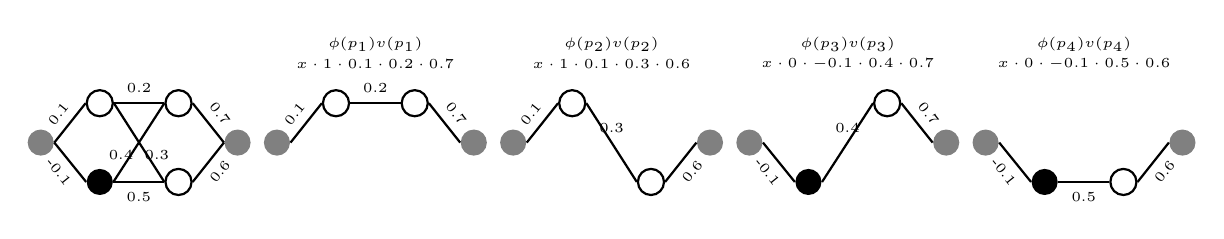
\begin{tikzpicture}
%Top Left
\node[draw,fill=white,circle,thick,
] (tl) at (-0.5,2){};

%Top Right
\node[draw,fill=white,circle,thick,
] (tr) at (0.5,2){};

%Bottom Left
\node[fill=black,circle,
] (bl) at (-0.5,1){};

%Bottom Right
\node[draw,fill=white,circle,thick,
] (br) at (0.5,1){};


%Input
\node[fill=gray,circle,
] (input) at (-1.25,1.5){};


%Output
\node[fill=gray,circle,
] (output) at (1.25,1.5){};

\draw[-, thick] (input.east) -- (tl.west) node [midway, above, sloped] (t1) {\tiny{0.1}};
\draw[-, thick] (input.east) -- (bl.west) node [midway, below, sloped] (t2) {\tiny{-0.1}};
\draw[-, thick] (tl.east) -- (tr.west) node [midway, above, sloped] (t1) {\tiny{0.2}};
\draw[-, thick] (bl.east) -- (br.west) node [midway, below, sloped] (t1) {\tiny{0.5}};
\draw[-, thick] (tl.east) -- (br.west) node [pos=0.85, above] (t1) {\tiny{0.3}};
\draw[-, thick] (bl.east) -- (tr.west) node [pos=0.15, above] (t1) {\tiny{0.4}};
\draw[-, thick] (tr.east) -- (output.west) node [midway, above, sloped] (t1) {\tiny{0.7}};
\draw[-, thick] (br.east) -- (output.west) node [midway, below, sloped] (t1) {\tiny{0.6}};




%%%%%%%%%%%%%%%%%Path 1%%%%%%%%%%%%%%
%Input
\node[fill=gray,circle,
] (p1input) at (1.75,1.5){};


%Output
\node[fill=gray,circle,
] (p1output) at (4.25,1.5){};



%Top Left
\node[draw,fill=white,circle,thick,
] (p1tl) at (2.5,2){};

%Top Right
\node[draw,fill=white,circle,thick,
] (p1tr) at (3.5,2){};




\draw[-, thick] (p1input.east) -- (p1tl.west) node [midway, above, sloped] (t1) {\tiny{0.1}};
\draw[-, thick] (p1tl.east) -- (p1tr.west) node [midway, above, sloped] (t1) {\tiny{0.2}};
\draw[-, thick] (p1tr.east) -- (p1output.west) node [midway, above, sloped] (t1) {\tiny{0.7}};



%%%%%%%%%%%%%%%%%Path 2%%%%%%%%%%%%%%

%Input
\node[fill=gray,circle,
] (p2input) at (4.75,1.5){};


%Output
\node[fill=gray,circle,
] (p2output) at (7.25,1.5){};

%Top Left
\node[draw,fill=white,circle,thick,
] (p2tl) at (5.5,2){};

%Bottom Right
\node[draw,fill=white,circle,thick,
] (p2br) at (6.5,1){};

\draw[-, thick] (p2input.east) -- (p2tl.west) node [midway, above, sloped] (t1) {\tiny{0.1}};
\draw[-, thick] (p2tl.east) -- (p2br.west) node [pos=0.5, above] (t1) {\tiny{0.3}};
\draw[-, thick] (p2br.east) -- (p2output.west) node [midway, below, sloped] (t1) {\tiny{0.6}};



%%%%%%%%%%%%%%%%%Path 3%%%%%%%%%%%%%%

%Input
\node[fill=gray,circle,
] (p3input) at (7.75,1.5){};


%Output
\node[fill=gray,circle,
] (p3output) at (10.25,1.5){};


%Top Right
\node[draw,fill=white,circle,thick,
] (p3tr) at (9.5,2){};

%Bottom Left
\node[fill=black,circle,
] (p3bl) at (8.5,1){};



\draw[-, thick] (p3input.east) -- (p3bl.west) node [midway, below, sloped] (t2) {\tiny{-0.1}};
\draw[-, thick] (p3bl.east) -- (p3tr.west) node [pos=0.5, above] (t1) {\tiny{0.4}};
\draw[-, thick] (p3tr.east) -- (p3output.west) node [midway, above, sloped] (t1) {\tiny{0.7}};


%%%%%%%%%%%%%%%%%Path 4%%%%%%%%%%%%%%

%Input
\node[fill=gray,circle,
] (p4input) at (10.75,1.5){};


%Output
\node[fill=gray,circle,
] (p4output) at (13.25,1.5){};

%Bottom Left
\node[fill=black,circle,
] (p4bl) at (11.5,1){};

%Bottom Right
\node[draw,fill=white,circle,thick,
] (p4br) at (12.5,1){};

\draw[-, thick] (p4input.east) -- (p4bl.west) node [midway, below, sloped] (t2) {\tiny{-0.1}};
\draw[-, thick] (p4bl.east) -- (p4br.west) node [midway, below, sloped] (t1) {\tiny{0.5}};
\draw[-, thick] (p4br.east) -- (p4output.west) node [midway, below, sloped] (t1) {\tiny{0.6}};
%%%%%%%%%%%%%%%%%%%%%%%%%%%%%%

\node[] () at (3,2.75){\tiny{$\phi(p_1)v(p_1)$}};
\node[] () at (3,2.5){\tiny{$x\cdot 1\cdot 0.1 \cdot 0.2 \cdot 0.7$}};

\node[] () at (6,2.75){\tiny{$\phi(p_2)v(p_2)$}};
\node[] () at (6,2.5){\tiny{$x\cdot 1\cdot 0.1 \cdot 0.3 \cdot 0.6$}};

\node[] () at (9,2.75){\tiny{$\phi(p_3)v(p_3)$}};
\node[] () at (9,2.5){\tiny{$x\cdot 0\cdot -0.1 \cdot 0.4 \cdot 0.7$}};

\node[] () at (12,2.75){\tiny{$\phi(p_4)v(p_4)$}};
\node[] () at (12,2.5){\tiny{$x\cdot 0\cdot -0.1 \cdot 0.5 \cdot 0.6$}};




\end{tikzpicture}


}
\caption{\small{Illustration of the dual `path-by-path' view of computations in a toy network with an input node, $2$ layer and $2$ hidden units in each layer and an output node. . Let us say for this particular input $x$, the bottom ReLU/gate in the first layer is `off/inactive' and rest of the ReLUs are `on/active'. In this case , paths $p_1$ and $p_2$ are active and paths $p_3$ and $p_4$ are inactive. }}
\label{fig:paths}
\end{figure}
\end{comment}
\subsubsection{Neural Path Feature, Value, Kernel and Deep Gated Network}
Consider a fully connected DNN with `$d$' layers and `$w$' hidden units in each layer. Let the DNN accept input $x\in \R^{\din}$ and produce an output $\hat{y}_{\Theta}(x)\in\R$. %Let a path be defined to be one that starts from an input node, passes through a weight and a hidden unit in each layer and ends at the output node. There are $\Pfc= \din w^{(d-1)}$ paths, let them be enumerable as $p=1,\ldots, \Pfc$. Let the index of the hidden unit in layer $l$ through which a path $p$ passes be denoted by $\I_l(p), l=0,1,\ldots,d$, where $l=0$ means the input layer. Let $\Theta\in\R^{\dnet}$ be the weights of network, with $\Theta(l,i,j)$ denoting the weight connecting the $i^{th}$ unit in layer $l$ and the $j^{th}$ unit in layer $l-1$. Let $G_l(x,I_l(p))$ denote the gate in the $l^{th}$ layer in path $p$. The neural path feature encoding the input and gates, and the neural path value encoding the weights is defined as below.
\begin{definition}\label{def:npf-npv}
A path starts from an input node, passes through a weight and a hidden unit in each layer and ends at the output node. We define the following quantities for a path $p$:
\begin{comment}
\begin{tabular}{lccl}
 Activity&:& $A_{\Theta}(x,p)$&=$\quad\Pi_{l=1}^{d-1} G_l\left(x,\I_l(p)\right)$.\\
Value&:& $v_{\Theta}(p)$&=$\quad\Pi_{l=1}^d\Theta\left(l,\I_{l-1}(p),\I_{l}(p)\right)$.\\
Feature&:&   $\phi_{\Theta}(x,p)$&=$\quad x\left(\I_0(p)\right)A_{\Theta}(x,p)$.
\end{tabular}
\end{comment}
\emph{
\begin{tabular}{lcl}
 Activity&:& $A_{\Theta}(x,p)$ is the product of the `$d-1$' gates in the path. \\
Value&:& $v_{\Theta}(p)$ is the product of the `$d$' weights in the path.\\
Feature&:&   $\phi_{\Theta}(x,p)$ is the product of the signal at the input node of the path and $A_{\Theta}(x,p)$.\\
\end{tabular}
}
The \emph{neural path feature} (NPF) given by $\phi_{\Theta}(x)=\left(\phi_{\Theta}(x,p),p=1,\ldots, \Pfc\right),\in\R^{\Pfc}$ and the \emph{neural path value} (NPV) given by $v_{\Theta}=\left(v_{\Theta}(p),p=1,\ldots,\Pfc\right),\in\R^{\Pfc}$, where $\Pfc=\din w^{(d-1)}$ is the total number of paths. 
\end{definition}
%Note that the neural path features are completely dictated by the gates, and i.e., if any gate in a path $p$ is not active for a given input $x\in\R^{\din}$, then $\phi(x,p)=0$.
\begin{proposition}\label{prop:npf-npv}
The output of the DNN is then the inner product of the NPF and NPV: 
\begin{align}\label{eq:inner}
\hat{y}_{\Theta}(x)=\ip{\phi_{\Theta}(x),v_{\Theta}}=\sum_{p\in[P]}  \phi_{\Theta}(x,p) v_{\Theta}(p)
\end{align}
\end{proposition}
\textbf{Subnetwork Interpretation of DNNs with ReLUs.} A path is active only if all the gates in the path are active. This gives a subnetwork interpretation, i.e., for a given input $x\in\R^{\din}$ only a subset of the gates and consequently only a subset of the paths are active, and the input to output computation can be seen to be produced by this active subnetwork. The following matrix captures the correlation of the active subnetworks for a given pair of inputs $x,x'\in\R^{\din}$.
\begin{definition}[Overlap of active sub-networks]\label{def:overlap} 
The total number of `active' paths for both $x$ and $x'$ that pass through input node $i$ is defined to be:

{\centering{$\textbf{overlap}_{\Theta}(i,x,x') \eqdef {\left|\{p \colon  p\,\text{starts at node}\, i \,, A_{\Theta}(x,p)= A_{\Theta}(x',p)=1\} \right|}$}\par}
\end{definition}
\begin{lemma}[Neural Path Kernel (NPK)]\label{lm:npk}
Let $D\in\R^{\din}$ be a vector of non-negative entries  and for $u,u'\in\R^{\din}$ , let $\ip{u,u'}_{D}=\sum_{i=1}^{\din}D(i)u(i)u'(i)$. Then the neural path kernel (NPK) is given by: 
\begin{align*} 
\text{NPK}_{\Theta}(x,x')\eqdef \ip{\phi_{\Theta}(x),\phi_{\Theta}(x')}= \ip{x,x'}_{\textbf{overlap}_{\Theta}(\cdot,x,x')} 
\end{align*}
\end{lemma}



%Each path transmits the signal equal to the neural path feature $\phi(x,p)$ which on its way to the output is scaled by the neural path value $v(p)$  which is equal the product of the weights in the path. 

\begin{comment}
\begin{figure}[t]
\centering
\resizebox{0.9\columnwidth}{!}{
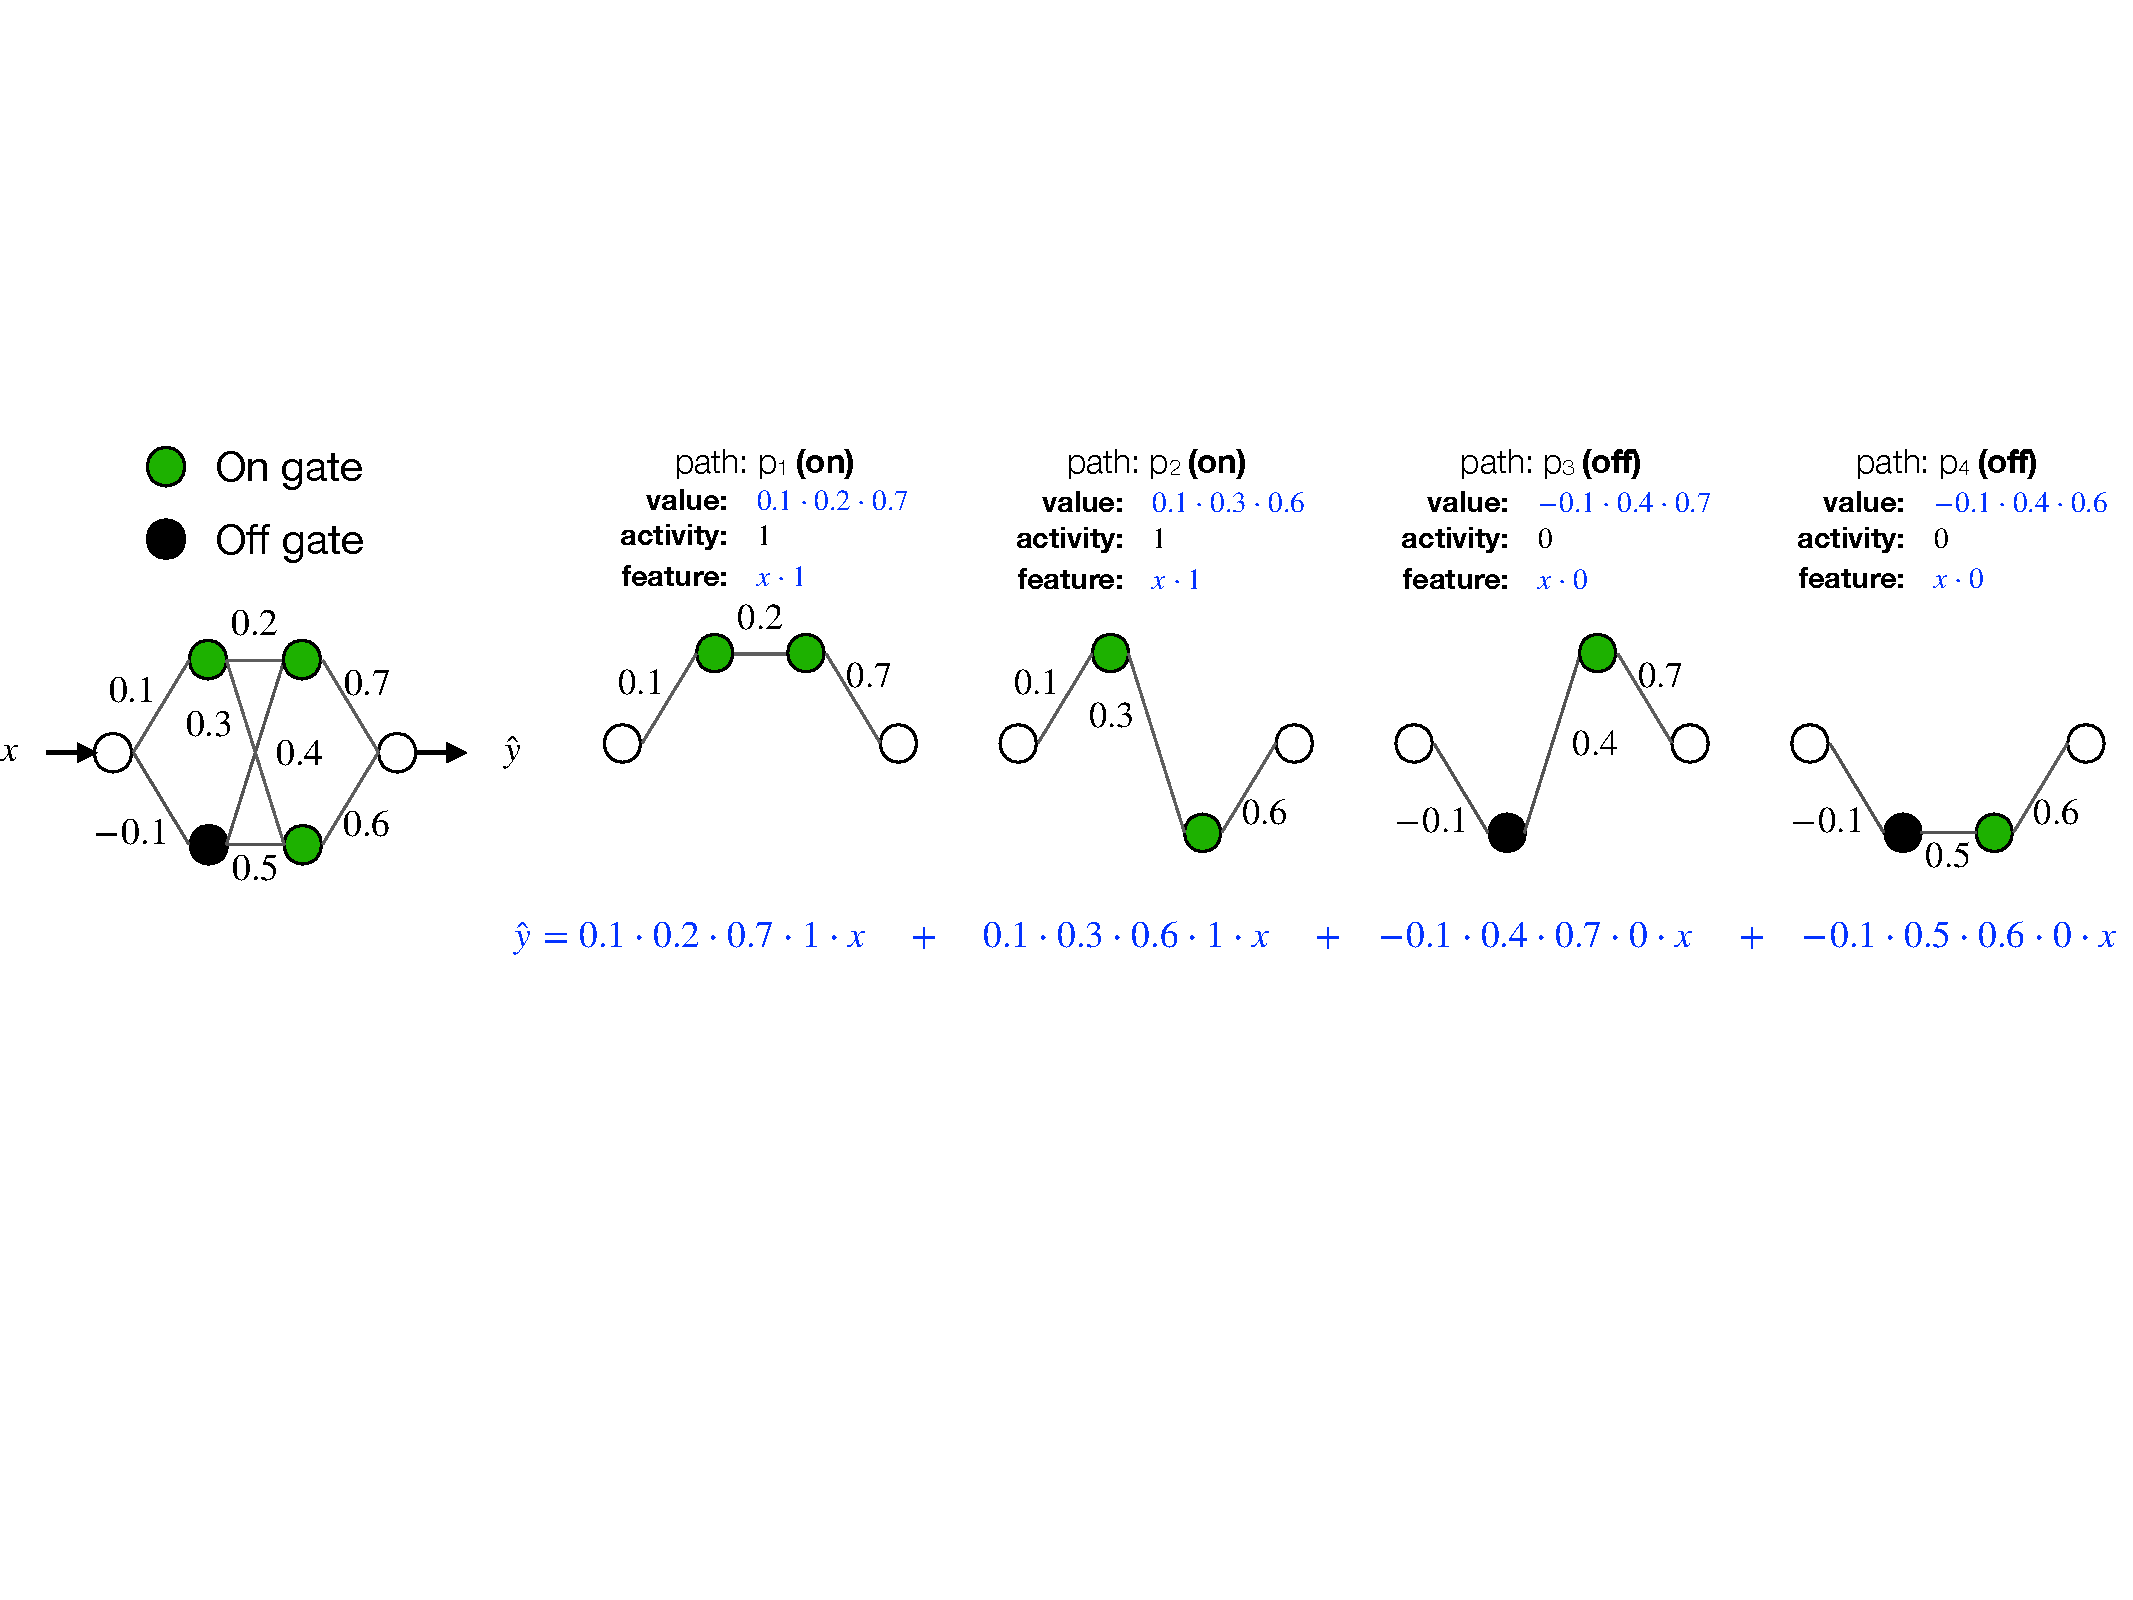
\includegraphics[scale=0.5]{figs/paths.pdf}
}
\caption{Illustration of \Cref{def:npf-npv} and \Cref{prop:npf-npv} in a  toy network with $2$ layers, $2$ gates per layer and $4$ paths. Paths $p_1$ and $p_2$ are `on' and paths $p_3$ and $p_4$ are `off'. The value, activity and feature of the individual paths are shown. $\hat{y}$ is the summation of the individual path contributions.}
\label{fig:paths}
\end{figure}

\begin{figure}
\centering
\begin{minipage}{0.9\columnwidth}
\begin{minipage}{0.49\columnwidth}
\resizebox{0.85\columnwidth}{!}{
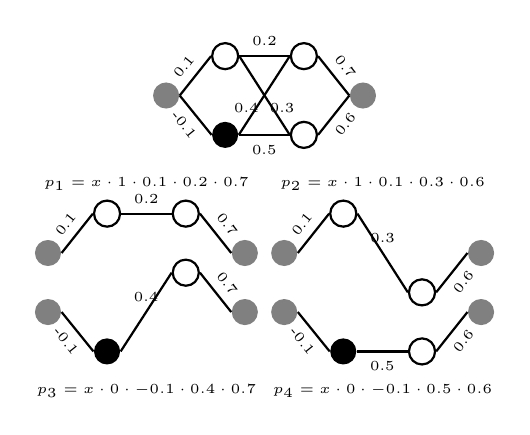
\begin{tikzpicture}
%Top Left
\node[draw,fill=white,circle,thick,
] (tl) at (-0.5,1.75){};

%Top Right
\node[draw,fill=white,circle,thick,
] (tr) at (0.5,1.75){};

%Bottom Left
\node[fill=black,circle,
] (bl) at (-0.5,0.75){};

%Bottom Right
\node[draw,fill=white,circle,thick,
] (br) at (0.5,0.75){};


%Input
\node[fill=gray,circle,
] (input) at (-1.25,1.25){};


%Output
\node[fill=gray,circle,
] (output) at (1.25,1.25){};

\draw[-, thick] (input.east) -- (tl.west) node [midway, above, sloped] (t1) {\tiny{0.1}};
\draw[-, thick] (input.east) -- (bl.west) node [midway, below, sloped] (t2) {\tiny{-0.1}};
\draw[-, thick] (tl.east) -- (tr.west) node [midway, above, sloped] (t1) {\tiny{0.2}};
\draw[-, thick] (bl.east) -- (br.west) node [midway, below, sloped] (t1) {\tiny{0.5}};
\draw[-, thick] (tl.east) -- (br.west) node [pos=0.85, above] (t1) {\tiny{0.3}};
\draw[-, thick] (bl.east) -- (tr.west) node [pos=0.15, above] (t1) {\tiny{0.4}};
\draw[-, thick] (tr.east) -- (output.west) node [midway, above, sloped] (t1) {\tiny{0.7}};
\draw[-, thick] (br.east) -- (output.west) node [midway, below, sloped] (t1) {\tiny{0.6}};




%%%%%%%%%%%%%%%%%Path 1%%%%%%%%%%%%%%
%Input
\node[fill=gray,circle,
] (p1input) at (-2.75,-0.750){};


%Output
\node[fill=gray,circle,
] (p1output) at (-0.25,-0.750){};



%Top Left
\node[draw,fill=white,circle,thick,
] (p1tl) at (-2.0,-0.25){};

%Top Right
\node[draw,fill=white,circle,thick,
] (p1tr) at (-1.0,-0.25){};




\draw[-, thick] (p1input.east) -- (p1tl.west) node [midway, above, sloped] (t1) {\tiny{0.1}};
\draw[-, thick] (p1tl.east) -- (p1tr.west) node [midway, above, sloped] (t1) {\tiny{0.2}};
\draw[-, thick] (p1tr.east) -- (p1output.west) node [midway, above, sloped] (t1) {\tiny{0.7}};



%%%%%%%%%%%%%%%%%Path 2%%%%%%%%%%%%%%

%Input
\node[fill=gray,circle,
] (p2input) at (0.25,-0.750){};


%Output
\node[fill=gray,circle,
] (p2output) at (2.75,-0.750){};

%Top Left
\node[draw,fill=white,circle,thick,
] (p2tl) at (1,-0.25){};

%Bottom Right
\node[draw,fill=white,circle,thick,
] (p2br) at (2,-1.25){};

\draw[-, thick] (p2input.east) -- (p2tl.west) node [midway, above, sloped] (t1) {\tiny{0.1}};
\draw[-, thick] (p2tl.east) -- (p2br.west) node [pos=0.5, above] (t1) {\tiny{0.3}};
\draw[-, thick] (p2br.east) -- (p2output.west) node [midway, below, sloped] (t1) {\tiny{0.6}};



%%%%%%%%%%%%%%%%%Path 3%%%%%%%%%%%%%%

%Input
\node[fill=gray,circle,
] (p3input) at (-2.75,-1.5){};


%Output
\node[fill=gray,circle,
] (p3output) at (-0.25,-1.5){};


%Top Right
\node[draw,fill=white,circle,thick,
] (p3tr) at (-1,-1){};

%Bottom Left
\node[fill=black,circle,
] (p3bl) at (-2,-2){};



\draw[-, thick] (p3input.east) -- (p3bl.west) node [midway, below, sloped] (t2) {\tiny{-0.1}};
\draw[-, thick] (p3bl.east) -- (p3tr.west) node [pos=0.5, above] (t1) {\tiny{0.4}};
\draw[-, thick] (p3tr.east) -- (p3output.west) node [midway, above, sloped] (t1) {\tiny{0.7}};


%%%%%%%%%%%%%%%%%Path 4%%%%%%%%%%%%%%

%Input
\node[fill=gray,circle,
] (p4input) at (0.25,-1.50){};


%Output
\node[fill=gray,circle,
] (p4output) at (2.75,-1.50){};

%Bottom Left
\node[fill=black,circle,
] (p4bl) at (1,-2){};

%Bottom Right
\node[draw,fill=white,circle,thick,
] (p4br) at (2,-2){};

\draw[-, thick] (p4input.east) -- (p4bl.west) node [midway, below, sloped] (t2) {\tiny{-0.1}};
\draw[-, thick] (p4bl.east) -- (p4br.west) node [midway, below, sloped] (t1) {\tiny{0.5}};
\draw[-, thick] (p4br.east) -- (p4output.west) node [midway, below, sloped] (t1) {\tiny{0.6}};


%%%%%%%%%%%%%%%%%%%%%%%%%%%%%%%%%%%%%%%%%%%%

\node[] () at (-1.5,0.125){\tiny{$p_1=x\cdot 1\cdot 0.1 \cdot 0.2 \cdot 0.7$}};

\node[] () at (1.5,0.125){\tiny{$p_2=x\cdot 1\cdot 0.1 \cdot 0.3 \cdot 0.6$}};

\node[] () at (-1.5,-2.5){\tiny{$p_3=x\cdot 0\cdot -0.1 \cdot 0.4 \cdot 0.7$}};

\node[] () at (1.5,-2.5){\tiny{$p_4=x\cdot 0\cdot -0.1 \cdot 0.5 \cdot 0.6$}};




\end{tikzpicture}


}
\end{minipage}
\begin{minipage}{0.49\columnwidth}
\resizebox{0.99\columnwidth}{!}{
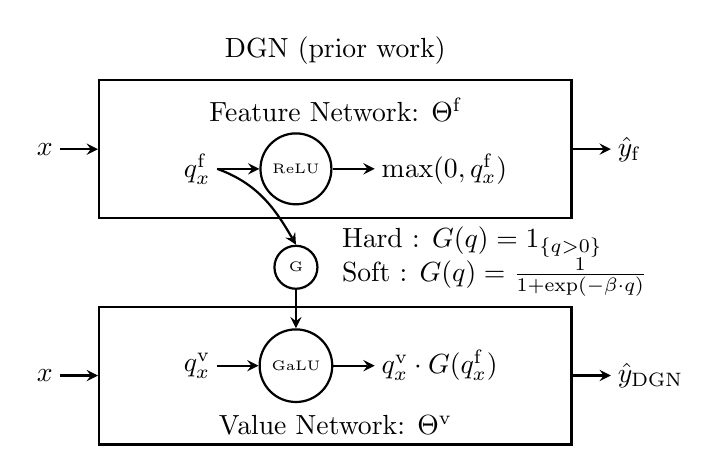
\begin{tikzpicture}

\node []  (fntext)at (3.5,1.5) {DGN (prior work)};
%Feature Network
\node [draw,
	minimum width=6cm,
	minimum height=1.75cm,
	thick
]  (fnbox)at (3.5,0.25) {};
\node []  (fntext)at (3.5,0.75) {Feature Network: $\Tf$};


%Feature Network Input
\node (fin) [left of=fnbox,node distance=3.5cm, coordinate] {};
\node[left=-1pt] at (fin.west){$x$};
\draw[-stealth, thick] (fin.center) -- (fnbox.west);

%Feature Network Output
\node (fout) [right of=fnbox,node distance=3.5cm, coordinate] {};
\node[right=-1pt] at (fout.west){$\hat{y}_{\text{f}}$};
\draw[-stealth, thick]  (fnbox.east)--(fout.center);


%ReLU Circle
\node[draw,
	circle,
	minimum size=0.75cm,thick,
] (relu) at (3,0){\tiny{ReLU}};
%ReLU Input
\node (b) [left of=relu,node distance=1cm, coordinate] {};

\node[left=-1pt] at (b.center){$q^\text{f}_x$};
\draw[-stealth, thick] (b.east) -- (relu.west);


%ReLU Output
\node (c) [right of=relu,node distance=1cm, coordinate] {};
\node[right=-1pt] at (c.center){$\max(0,q^\text{f}_x)$};
\draw[-stealth, thick] (relu.east) -- (c.west);
	

%Gating Circle
\node[draw,
	circle,
	minimum size=0.0625cm,thick,
] (gating) at (3,-1.25){\tiny{G}};
%\node[right=6pt] at (gating.north){Hard : $G(q)=\mathbbm{1}_{\{q>0\}} $};
%\node[below right=6pt] at (gating.north){Soft : $G(q)=\frac{1}{1+\exp(-\beta\cdot q)}$};

\node[right=6pt] at (3.25,-0.925){Hard : $G(q)=\mathbbm{1}_{\{q>0\}} $};
\node[right=6pt] at (3.25,-1.375){Soft : $G(q)=\frac{1}{1+\exp(-\beta\cdot q)}$};


%Value Network

\node [draw,
	minimum width=6cm,
	minimum height=1.75cm,
	thick
]  (vnbox)at (3.5,-2.625) {};

\node []  (vntext)at (3.5,-3.25) {Value Network: $\Tv$};

%Value Network Input
\node (vin) [left of=vnbox,node distance=3.5cm, coordinate] {};
\node[left=-1pt] at (vin.west){$x$};
\draw[-stealth, thick] (vin.center) -- (vnbox.west);

%Feature Network Input
\node (vout) [right of=vnbox,node distance=3.5cm, coordinate] {};
\node[right=-1pt] at (vout.west){$\hat{y}_{\text{DGN}}$};
\draw[-stealth, thick]  (vnbox.east)--(vout.center);



%GaLU Circle
\node[draw,
	circle,
	minimum size=0.75cm,thick,
] (galu) at (3,-2.5){\tiny{GaLU}};

\draw [-stealth,thick]   (b) to[out=-20,in=120] (gating.north);
\draw [-stealth,thick]   (gating.south) -- (galu.north);


%GaLU Input
\node (d) [left of=galu,node distance=1cm, coordinate] {};
\node[left=-1pt] at (d.center){$q^\text{v}_x$};
\draw[-stealth, thick] (d.east) -- (galu.west);
%GaLU Output
\node (e) [right of=galu,node distance=1cm, coordinate] {};
\node[right=-1pt] at (e.center){$q^\text{v}_x\cdot G(q^\text{f}_x)$};
\draw[-stealth, thick] (galu.east) -- (e.west);
	
\end{tikzpicture}


}
\end{minipage}
\end{minipage}
\caption{DGN}
\label{fig:dgn}
\end{figure}
\end{comment}
\begin{figure}
\centering
\begin{minipage}{0.9\columnwidth}
\centering
\begin{minipage}{0.45\columnwidth}
\resizebox{1.0\columnwidth}{!}{
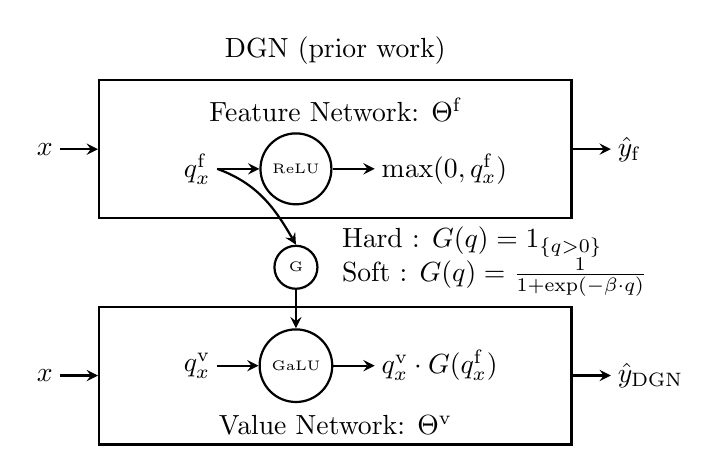
\begin{tikzpicture}

\node []  (fntext)at (3.5,1.5) {DGN (prior work)};
%Feature Network
\node [draw,
	minimum width=6cm,
	minimum height=1.75cm,
	thick
]  (fnbox)at (3.5,0.25) {};
\node []  (fntext)at (3.5,0.75) {Feature Network: $\Tf$};


%Feature Network Input
\node (fin) [left of=fnbox,node distance=3.5cm, coordinate] {};
\node[left=-1pt] at (fin.west){$x$};
\draw[-stealth, thick] (fin.center) -- (fnbox.west);

%Feature Network Output
\node (fout) [right of=fnbox,node distance=3.5cm, coordinate] {};
\node[right=-1pt] at (fout.west){$\hat{y}_{\text{f}}$};
\draw[-stealth, thick]  (fnbox.east)--(fout.center);


%ReLU Circle
\node[draw,
	circle,
	minimum size=0.75cm,thick,
] (relu) at (3,0){\tiny{ReLU}};
%ReLU Input
\node (b) [left of=relu,node distance=1cm, coordinate] {};

\node[left=-1pt] at (b.center){$q^\text{f}_x$};
\draw[-stealth, thick] (b.east) -- (relu.west);


%ReLU Output
\node (c) [right of=relu,node distance=1cm, coordinate] {};
\node[right=-1pt] at (c.center){$\max(0,q^\text{f}_x)$};
\draw[-stealth, thick] (relu.east) -- (c.west);
	

%Gating Circle
\node[draw,
	circle,
	minimum size=0.0625cm,thick,
] (gating) at (3,-1.25){\tiny{G}};
%\node[right=6pt] at (gating.north){Hard : $G(q)=\mathbbm{1}_{\{q>0\}} $};
%\node[below right=6pt] at (gating.north){Soft : $G(q)=\frac{1}{1+\exp(-\beta\cdot q)}$};

\node[right=6pt] at (3.25,-0.925){Hard : $G(q)=\mathbbm{1}_{\{q>0\}} $};
\node[right=6pt] at (3.25,-1.375){Soft : $G(q)=\frac{1}{1+\exp(-\beta\cdot q)}$};


%Value Network

\node [draw,
	minimum width=6cm,
	minimum height=1.75cm,
	thick
]  (vnbox)at (3.5,-2.625) {};

\node []  (vntext)at (3.5,-3.25) {Value Network: $\Tv$};

%Value Network Input
\node (vin) [left of=vnbox,node distance=3.5cm, coordinate] {};
\node[left=-1pt] at (vin.west){$x$};
\draw[-stealth, thick] (vin.center) -- (vnbox.west);

%Feature Network Input
\node (vout) [right of=vnbox,node distance=3.5cm, coordinate] {};
\node[right=-1pt] at (vout.west){$\hat{y}_{\text{DGN}}$};
\draw[-stealth, thick]  (vnbox.east)--(vout.center);



%GaLU Circle
\node[draw,
	circle,
	minimum size=0.75cm,thick,
] (galu) at (3,-2.5){\tiny{GaLU}};

\draw [-stealth,thick]   (b) to[out=-20,in=120] (gating.north);
\draw [-stealth,thick]   (gating.south) -- (galu.north);


%GaLU Input
\node (d) [left of=galu,node distance=1cm, coordinate] {};
\node[left=-1pt] at (d.center){$q^\text{v}_x$};
\draw[-stealth, thick] (d.east) -- (galu.west);
%GaLU Output
\node (e) [right of=galu,node distance=1cm, coordinate] {};
\node[right=-1pt] at (e.center){$q^\text{v}_x\cdot G(q^\text{f}_x)$};
\draw[-stealth, thick] (galu.east) -- (e.west);
	
\end{tikzpicture}


}
\end{minipage}
\begin{minipage}{0.54\columnwidth}
\resizebox{1.0\columnwidth}{!}{
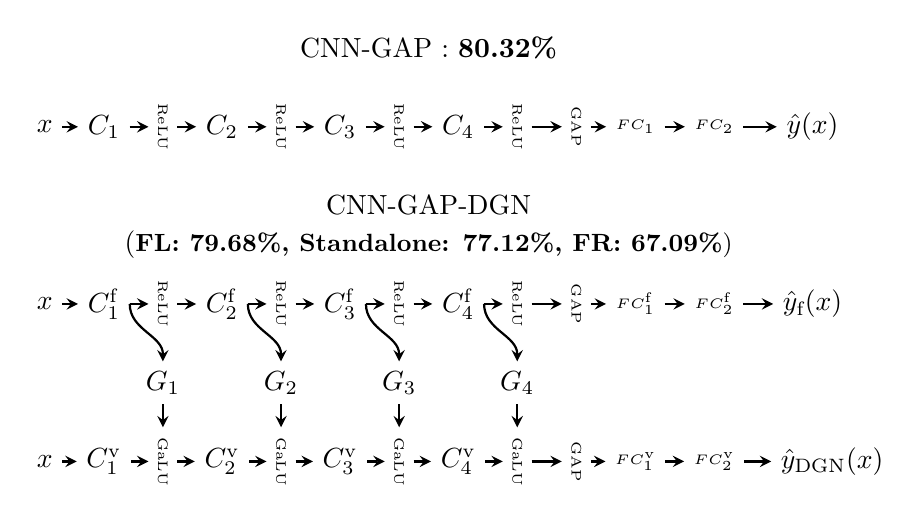
\begin{tikzpicture}
\node []  (dnn-text)at (5.375,2) {CNN-GAP : \textbf{80.32\%}};

\node []  (dnn-output) at (10.25,1) {$\hat{y}(x)$};
\node []  (dnn-fc2) at (9.0,1) {\tiny{$FC_2$}};
\draw [-stealth,thick]   (dnn-fc2.east) -- (dnn-output.west);

\node []  (dnn-fc1) at (8,1) {\tiny{$FC_1$}};
\draw [-stealth,thick]   (dnn-fc1.east) -- (dnn-fc2.west);

\node [rotate=-90]  (dnn-gap) at (7.25,1) {\tiny{GAP}};
\draw [-stealth,thick]   (dnn-gap.north) -- (dnn-fc1.west);

\node [rotate=-90] (dnn-relu-4) at (6.5,1){\tiny{ReLU}};
\node [] (dnn-c4) at (5.75,1){{$C_4$}};
\draw [-stealth,thick]   (dnn-c4.east) -- (dnn-relu-4.south);
\draw [-stealth,thick]   (dnn-relu-4.north) -- (dnn-gap.south);



\node [rotate=-90] (dnn-relu-3) at (5,1){\tiny{ReLU}};
\node [] (dnn-c3) at (4.25,1){{$C_3$}};
\draw [-stealth,thick]   (dnn-c3.east) -- (dnn-relu-3.south);
\draw [-stealth,thick]   (dnn-relu-3.north) -- (dnn-c4.west);


\node [rotate=-90] (dnn-relu-2) at (3.5,1){\tiny{ReLU}};
\node [] (dnn-c2) at (2.75,1){{$C_2$}};
\draw [-stealth,thick]   (dnn-c2.east) -- (dnn-relu-2.south);
\draw [-stealth,thick]   (dnn-relu-2.north) -- (dnn-c3.west);

\node [rotate=-90] (dnn-relu-1) at (2,1){\tiny{ReLU}};
\node [] (dnn-c1) at (1.25,1){{$C_1$}};
\draw [-stealth,thick]   (dnn-c1.east) -- (dnn-relu-1.south);
\draw [-stealth,thick]   (dnn-relu-1.north) -- (dnn-c2.west);



\node [] (dnn-input) at (0.5,1){$x$};
\draw [-stealth,thick]   (dnn-input.east) -- (dnn-c1.west);


%%%%%%%%%%%%%%%%%%%%%%%%%%%%%%%%%%%%%%%%%%%%%%%%%%%%%%%%%%%%%%%%%
\node []  (fntext)at (5.375,0) {CNN-GAP-DGN};
\node []  (fntext)at (5.375,-.5) {(\small{\textbf{FL: 79.68\%, Standalone: 77.12\%, FR: 67.09\%}})};

%\node []  (output) at (7.5,1.5) {$\hat{y}(x)$};


\node [align=right]  (dgn-f-output) at (10.25,-1.25) {$\hat{y}_{\text{f}}(x)$};
\node []  (dgn-f-fc2) at (9.0,-1.25) {\tiny{$FC^{\text{f}}_2$}};
\draw [-stealth,thick]   (dgn-f-fc2.east) -- (dgn-f-output.west);


\node []  (dgn-f-fc1) at (8,-1.25) {\tiny{$FC^{\text{f}}_1$}};
\draw [-stealth,thick]   (dgn-f-fc1.east) -- (dgn-f-fc2.west);




\node [rotate=-90]  (dgn-f-gap) at (7.25,-1.25) {\tiny{GAP}};
\draw [-stealth,thick]   (dgn-f-gap.north) -- (dgn-f-fc1.west);


\node [rotate=-90] (dgn-relu-4) at (6.5,-1.25){\tiny{ReLU}};
\node [] (dgn-f-c4) at (5.75,-1.25){{$C^{\text{f}}_4$}};
\draw [-stealth,thick]   (dgn-f-c4.east) -- (dgn-relu-4.south);
\draw [-stealth,thick]   (dgn-relu-4.north) -- (dgn-f-gap.south);


\node [rotate=-90] (dgn-relu-3) at (5,-1.25){\tiny{ReLU}};
\node [] (dgn-f-c3) at (4.25,-1.25){{$C^{\text{f}}_3$}};
\draw [-stealth,thick]   (dgn-f-c3.east) -- (dgn-relu-3.south);
\draw [-stealth,thick]   (dgn-relu-3.north) -- (dgn-f-c4.west);


\node [rotate=-90] (dgn-relu-2) at (3.5,-1.25){\tiny{ReLU}};
\node [] (dgn-f-c2) at (2.75,-1.25){{$C^{\text{f}}_2$}};
\draw [-stealth,thick]   (dgn-f-c2.east) -- (dgn-relu-2.south);
\draw [-stealth,thick]   (dgn-relu-2.north) -- (dgn-f-c3.west);


\node [rotate=-90] (dgn-relu-1) at (2,-1.25){\tiny{ReLU}};
\node [] (dgn-f-c1) at (1.25,-1.25){{$C^{\text{f}}_1$}};
\draw [-stealth,thick]   (dgn-f-c1.east) -- (dgn-relu-1.south);
\draw [-stealth,thick]   (dgn-relu-1.north) -- (dgn-f-c2.west);



\node [] (dgn-f-input) at (0.5,-1.25){$x$};
\draw [-stealth,thick]   (dgn-f-input.east) -- (dgn-f-c1.west);

\node [align=right]  (dgn-output) at (10.5,-3.25) {$\hat{y}_{\text{DGN}}(x)$};

\node [] (dgn-fc2) at (9,-3.25){\tiny{$FC^{\text{v}}_2$}};
\draw [-stealth,thick]   (dgn-fc2.east)--(dgn-output.west);

\node [] (dgn-fc1) at (8,-3.25){\tiny{$FC^{\text{v}}_1$}};
\draw [-stealth,thick]   (dgn-fc1.east)--(dgn-fc2.west);

\node [rotate=-90] (dgn-gap) at (7.25,-3.25){\tiny{GAP}};
\draw [-stealth,thick]   (dgn-gap.north)--(dgn-fc1.west);



\node [rotate=-90] (dgn-galu-4) at (6.5,-3.25){\tiny{GaLU}};
\draw [-stealth,thick]   (dgn-galu-4.north) -- (dgn-gap.south);

\node [] (dgn-v-c4) at (5.75,-3.25){{$C^{\text{v}}_4$}};
\draw [-stealth,thick]   (dgn-v-c4.east) -- (dgn-galu-4.south);

\node [rotate=-90] (dgn-galu-3) at (5,-3.25){\tiny{GaLU}};
\node [] (dgn-v-c3) at (4.25,-3.25){{$C^{\text{v}}_3$}};
\draw [-stealth,thick]   (dgn-v-c3.east) -- (dgn-galu-3.south);
\draw [-stealth,thick]   (dgn-galu-3.north) -- (dgn-v-c4.west);



\node [rotate=-90] (dgn-galu-2) at (3.5,-3.25){\tiny{GaLU}};
\node [] (dgn-v-c2) at (2.75,-3.25){{$C^{\text{v}}_2$}};
\draw [-stealth,thick]   (dgn-v-c2.east) -- (dgn-galu-2.south);
\draw [-stealth,thick]   (dgn-galu-2.north) -- (dgn-v-c3.west);


\node [rotate=-90] (dgn-galu-1) at (2,-3.25){\tiny{GaLU}};
\node [] (dgn-v-c1) at (1.25,-3.25){{$C^{\text{v}}_1$}};

\draw [-stealth,thick]   (dgn-v-c1.east) -- (dgn-galu-1.south);
\draw [-stealth,thick]   (dgn-galu-1.north) -- (dgn-v-c2.west);




\node [] (dgn-input) at (0.5,-3.25){$x$};
\draw [-stealth,thick]   (dgn-input.east) -- (dgn-v-c1.west);




\node[] (dgn-gating-1) at (2,-2.25){$G_1$};
\draw [-stealth,thick]   (dgn-f-c1.east) to[out=-90,in=90] (dgn-gating-1.north);
\draw [-stealth,thick]   (dgn-gating-1.south) -- (dgn-galu-1.west);


\node[] (dgn-gating-2) at (3.5,-2.25){$G_2$};
\draw [-stealth,thick]   (dgn-f-c2.east) to[out=-90,in=90] (dgn-gating-2.north);
\draw [-stealth,thick]   (dgn-gating-2.south) -- (dgn-galu-2.west);



\node[] (dgn-gating-3) at (5,-2.25){$G_3$};
\draw [-stealth,thick]   (dgn-f-c3.east) to[out=-90,in=90] (dgn-gating-3.north);
\draw [-stealth,thick]   (dgn-gating-3.south) -- (dgn-galu-3.west);


\node[] (dgn-gating-4) at (6.5,-2.25){$G_4$};
\draw [-stealth,thick]   (dgn-f-c4.east) to[out=-90,in=90] (dgn-gating-4.north);
\draw [-stealth,thick]   (dgn-gating-4.south) -- (dgn-galu-4.west);

	
\end{tikzpicture}


}
\end{minipage}
\end{minipage}
\caption{\small{Shows the DGN on the left. \textbf{Training:} In the case of fixed learnt gates, the feature network is pre-trained using $\hat{y}_f$ as the output, and then the feature network is frozen, and the value network is trained with $\hat{y}_{DGN}$ as the output. In the case of fixed random gates, the feature network is initialised at random and frozen, and the value network is trained with $\hat{y}_{DGN}$ as the output. In the case of fixed gates hard gating $G(q)=\mathbbm{1}_{\{q>0\}}$ is used. For standalone training, both feature and value network are initialised at random and trained together with $\hat{y}_{DGN}$ as the output. Here, soft gating $G(q)=\frac{1}{1+\exp(-\beta\cdot q)}$ is used to allow gradient flow through feature network. On the right side is the CNN-GAP and its DGN used in \citep{npk}. In CNN-GAP, $C_1,C_2,C_3,C_4$ are convolutional layers, $FC_1,FC_2$ are fully connected layers. In CNN-GAP-DGN, $G_l, l=1,2,3,4$ are the gates of layers, the superscripts f, and v stand for feature and value network respectively.}}
\label{fig:dgn}
\end{figure}

%As mentioned in \Cref{sec:intro}, a deep gated network(DGN) setup is an alternative way to compute path-by-path, that is, the to compute the inner product of the neural path feature and neural path value. In this section, we first describe DGN in prior work \citep{npk}:  consitituent parts, information flow, purpose and training. We then discuss the two fundamental conceptual issues that make this DGN `black box'. We then present our modified \texttt{DGN-NO-ACT} with an intutitve explanation of how the conceptual issues are overcome and  why it is an entirely interpretatble white box model. These intuitive explanations will be justified in theory and experiments in \Cref{sec:main}.
%\subsubsection{Deep Gated Network: Separating Gates and Weights}
\textbf{Deep Gated Network (DGN)} is a setup to separate the gates from the weights. Consider a DNN with ReLUs with weights $\Theta\in\R^{\dnet}$. The DGN \emph{corresponding} to this DNN (left diagram in \Cref{fig:dgn}) has two networks of \emph{identical architecture} (to the DNN) namely the `gating network' and the `weight network' with distinct weights $\Tf\in\R^{\dnet}$ and $\Tv\in\R^{\dnet}$.  
%The main difference between the feature and value networks is in the activations. 
The `gating network' has ReLUs which turn `on/off' based on their pre-activation signals, and the `weight network' has gated linear units (GaLUs) \citep{sss,npk}, which multiply their respective pre-activation inputs by the external gating signals provided by the `gating network'.  Since both the networks have identical architecture, the ReLUs and GaLUs in the respective networks have a one-to-one correspondence.  Gating network realises $\phi_{\Tf}(x)$ by turning `on/off' the corresponding GaLUs in the weight network. The weight network realises $v_{\Tv}$ and computes the output $\hat{y}_{\text{DGN}}(x)=\ip{\phi_{\Tf}(x),v_{\Tv}}$.  The gating network is also called as the feature network since it realises the neural path features, and the weight network is also called as the value network since it realises the neural path value. %Training of DGN is explained in \Cref{sec:gatelearning}.

%In the DGN, the external gating signal to the GaLU is derived from the pre-activation input of the corresponding ReLU. 

%The feature network computes the pre-activations in a layer-by-layer manner, the pre-activations from the feature network generate the gates, which are then used to switch

\subsubsection{Learning Weights With Fixed Gates = Neural Path Kernel}\label{sec:fixedgates}
During training, a DNN learns both $\phi_{\Theta}(x)$ as well as $v_{\Theta}$ simultaneously, and a finite time characterisation of this learning in finite width DNNs is desirable. However, this is a hard problem. An easier problem is to understand in a DGN, how the weights in the value network are learnt when the gates are fixed in the feature network, i.e., how $\hat{y}_{DGN}(x)=\ip{\phi_{\Tf}(x),v_{\Tv}}$ is learnt by learning $v_{\Tv}$ with fixed $\phi_{\Tf}(x)$. While  $\hat{y}_{DGN}(x)=\ip{\phi_{\Tf}(x),v_{\Tv}}$ is linear in the dual variables, it is still non-linear in the value network weights $\Tv$. However, \cite{npk} showed that the dual linearity is characterised by the NPK in the infinite width regime. We state the assumption followed by Theorem 5.1 in \citep{npk}, wherein, the $\text{NTK}(x,x')=\ip{\nabla_{\Tv}\hat{y}_{\Tdgn_0}(x),\nabla_{\Tv}\hat{y}_{\Tdgn_0}(x') }$ is due to the gradient of $\hat{y}_{\text{DGN}}$ with respect to the value network weights, and the $\text{NPK}(x,x')=\ip{\phi_{\Tf_0}(x),\phi_{\Tf_0}(x')}$ is due to the feature network weights.

\begin{assumption}\label{assmp:main}
$\Tv_0\stackrel{\text{i.i.d}}\sim\text{Bernoulli}(\frac12)$ over $\{-{\sigma},+{\sigma}\}$ and statistically independent of $\Tf_0$.
\end{assumption}
%We point out that this statistical decoupling of weights and gates in \Cref{assmp:main} is unrealisable in a DNN with ReLU, however, this assumption can be trivially realised in a DGN. %Further, we are interested only in the `what?' ( and not `how?') question related to the gates in which case this assumptions is not a restriction.

\begin{theorem}[Theorem 5.1 in \citep{npk}]
\label{th:fcprev} Under \Cref{assmp:main} for a fully connected DGN : 
\begin{align*}
\text{NTK}^{\texttt{FC}}(x,x')\,\, \stackrel{(a)}\rightarrow\,\, &d \cdot \sigma^{2(d-1)} \cdot \text{NPK}^{\texttt{FC}}(x,x'), \quad\text{as}\,\, w\rightarrow \infty \\
					     & = d \cdot \sigma^{2(d-1)}\cdot\ip{x,x'}\cdot \textbf{overlap}(x,x')
\end{align*}
\end{theorem} 
\textbf{Remark.} In the fully connected case, $\textbf{overlap}(i,x,x')$ is identical for all $i=1,\ldots,\din$, and hence $\ip{x,x'}_{\textbf{overlap}(\cdot,x,x')}$ in \Cref{lm:npk} becomes $\ip{x,x'}\cdot \textbf{overlap}(x,x')$ in \Cref{th:fcprev}. It follows from NTK theory that, an infinite width DGN with fixed gates is equivalent to kernel method with NPK.
\subsubsection{Learning in Gates Key For Finite Width To Be Better Than Infinite Width}\label{sec:gatelearning}
The fixed gates setting is an idealised setting, in that, it does not theoretically capture the learning of the gates, i.e., the neural path features $\phi_{\Theta}(x)$. However, the learning in the gates can be empirically characterised by comparing \textbf{fixed learnt (FL)}  gates coming from a pre-trained DNN and \textbf{fixed random (FR)} gates coming from randomly initialised DNN, and the infinite width NTK.  Using a CNN-GAP and its corresponding DGN, \cite{npk} showed on CIFAR-10 that (see \Cref{fig:dgn} for details on DGN training and the CNN-GAP architecture):

{\centering FR Gates : $\mathbf{67.09\%}\leq $ CNTK-GAP: $\mathbf{77.43\%}\leq $ FL Gates: $\mathbf{79.68\%}\approx $ CNN-GAP: $\mathbf{80.32\%}$\par}

based on which it was concluded that learning in the gates (i.e., neural path features) is crucial for finite width CNN-GAP to outperform the infinite width CNTK-GAP.% this \textbf{explains the open question} in \Cref{sec:ntk}.
%Since the fixed random (FR) gates performed poorly ($67.09\%$) than the best CNTK in \citep{arora2019exact} ($77.43\%$) and the fixed learnt (FL) gates performed better ($79.68\%$) than the best CNTK, 

\textbf{Note.} Since the fixed learnt gates ($79.68\%$) recover almost all the performance of the DNN ($80.32\%$), it follows that most crucial learning happens in the gates. It was also shown that the DGN can be trained standalone if the gates allowed to learn along with the weights; standalone DGN is only \emph{marginally poor} compared to the DNN as shown in \Cref{fig:dgn}. 
%In other words, dual linearity is not a mere conceptualisation, but is analogous to a linear model in practice as well. That is, just like one can learn weight vector in a linear model given the features, one can learn the neural path value given the neural path features.
 \begin{comment}
\begin{table}
\begin{tabularx}{\columnwidth}{c *{4}{Y}}
\toprule 
CNN-GAP & \multicolumn{3}{c} {CDGN-GAP} \\\cline{2-4}
& Fixed Learnt Gates & Fixed Random Gates & Learnable Gates\\
80.32\% & 79.68\% &67.09\% & 77.12\%\\
\bottomrule
\end{tabularx}
\caption{Data from Table 2 in \citep{npk}.}
\label{tb:cdgn}
\end{table}
\end{comment}
%The information in the gates or the performance of the gates is measured by keeping the gates fixed in the feature network and training the weights of the value network. The key result in \citep{npk} was that the learning in the gates (i.e., the neural path features) improves generalisation, and is the reason behind why finite width DNNs outperforms the infinite width NTK. This result was established empirically by comparing the performance of \textbf{fixed learnt (FL)} gates and that of \textbf{fixed random(FR)} gates and the performance of the NTK in \cite{arora2019exact}. The fixed learnt gates are those that come from a pre-trained feature network (pre-trained using $\hat{y}_\text{f}$) and the fixed random gates are those that come from a randomly initialised feature network. For this purpose, \citep{npk} used a `C4GAP' architecture with $4$ convolutional layers, followed by global-average-pooling (GAP) and a fully connected layer with `softmax' activations. On CIFAR-10, it was observed that the fixed random (FR) gates performed poorly ($68.08\%$) than the NTK in \citep{arora2019exact} ($77.43$) and the fixed learnt (FL) gates performed better ($79.68\%$) than the NTK and within $1\%$ to the C4GAP-DNN ($80.32\%$). Based on this observation it was concluded that (i) gates (encoded as neural path features) are learnt, and (ii) the learning in the gates is the reason for finite width DNN outperforming infinite width NTK. It was also shown that the DGN can be trained standalone, i.e., gates in the feature network and the weights in the value network can be learnt starting from randomised initialisation. The standalone DGN performed only \emph{marginally poor} ($77.12\%$) compared to the DNN ($80.32\%$).

%The test accuracy of C4GAP is approximately $80\%$ on CIFAR-10, and is not state of the art.  However, the main aim here was to compare with the corresponding infinite width NTK whose performance was $77.34\%$ \citep{arora2019exact} for which the C4GAP was sufficient. 



%In a DNN with ReLUs, both the gates (encoded in the neural path features) and the weights (encoded in the neural path value) are learnt by the DNN itself. The DGN setup helps to separate out the learning in the gates (which are learnt in the feature network) and  from the learning in the weights (which are learnt in the value network). Using the DGN, the information in the gates can be measured, by keeping the gates fixed and then training the weights alone. This is equivalent to asking `how good are the neural path features?' and answering it by keeping $\phi_{\Tf}(x)$ fixed and training $v_{\Tv}$ to learn the relation $\hat{y}_{\text{DGN}}(x)=\ip{\phi_{\Tf}(x),v_{\Tv}}$. We now briefly main result in \citep{npk} on fixing gates and learning weights.

%{\centering \emph{{What is the analysis for fixing the gates, i.e., $\phi_{\Tf}(x)$ and learning the weights, i.e., $v_{\Tv}$?}}\par}

%\textbf{Analytical Characterisation of Learning Weights Given Gates.} Recent works \citep{ntk,arora2019exact,cao2019generalization} have connected the training and generalisation of DNNs to kernel methods. An important kernel associated with a DNN is its \emph{neural tangent kernel} (NTK), which, for a pair of input examples $x,x'\in\R^{\din}$, and network weights $\Theta\in\R^{\dnet}$, is given by:
%\begin{align*}
% \text{NTK}(x,x')\quad = \quad \ip{\nabla_{\Theta}\hat{y}(x), \nabla_{\Theta}\hat{y}(x')}
% \end{align*}
%It was shown that, as the width of the DNN goes to infinity, the NTK matrix converges to a limiting deterministic matrix $\text{NTK}_{\infty}$, and training an infinitely wide DNN is equivalent to a kernel method with $\text{NTK}_{\infty}$. Theorem 5.1 in \citep{npk} showed that, when the gates are fixed,  at randomised initialisation, the NTK of an  infinitely wide DGN is equal to (but for a constant factor) the neural path kernel (NPK) which is the Gram matrix of the neural path features. 

%\textbf{Remark:} A previously unnoticed property of the NPK was that it is invariant to layer permutations. Theorem 5.1 in \citep{npk} is not presented here, it is restated in \Cref{th:fc} in which the invariance property is made explicit. 



%\cite{npk} addressed these issues by measuring the performance of the fixed gates. For this, they considered a DGN setup, wherein, the feature network is frozen so as to fix the gates and only the value network is trained. In other words, the gates are fixed the `path features' are fixed, only the `path value' is learnt in the value network. 
%As mention in \Cref{sec:intro}, the key insight in \cite{npk} is that gates play an important role in DNNs with ReLUs. The DGN has external gating, i.e., gates are generated in the feature network and are external to the value network which learns the weights. Note that the neural path features encode the input and the gates, and in the context of DGN, we will be using neural path features as a synonym for the gates. Also the neural path value is learnt in the value network, and in the context of the DGN, we will use neural path value as a synonym for weights. The following question related to learning with external gating lead to the conclusion that gates are key.

%During training, a DNN learns the relation $\hat{y}(x)=\ip{\phi_\Theta(x),v_\Theta}$, i.e., it learns both the neural path features and value. The DGN separately stores $\phi(x)$ and $v$ in the feature and value network respectively and helps in understanding their roles separately.  
%if the feature network weights are fixed, then the gates are fixed and hence the neural path features are fixed as well. 
%Now, training the value network after fixing the gates is linear in the dual variables, and we call this \textbf{dual linearity}. In other words, $\hat{y}_{\text{DGN}}(x)=\ip{\phi_{\Tf}(x),v_{\Tv}}$, is a linear model, where the neural path feature $\phi_{\Tf}(x)\in\R^{\text{total\,paths}}$ is given, and the neural path value $v_{\Tv}\in\R^{\text{total\,paths}}$ needs to be learnt. However, unlike a linear model the various coordinates of $v_{\Tv}$ are not independent variables, but are dependent on each other through the weights (see \Cref{def:npf-npv}). Thus the relation $\hat{y}_{\text{DGN}}(x)=\ip{\phi_{\Tf}(x),v_{\Tv}}$, is non-linear in the weights of the value network. This brings us to the following natural questions, which were answered using the DGN setup:


%The dual view provides the first step in disentangling the linear and the non-linear operations. To elaborate,  it is worthwhile to ask `assuming that we have the \emph{right} neural path features $\phi_{\Tf}(x)$, then can we learn $v_{\Tv}$ separately?'.  This question is worthwhile because, while in each layer of the value network GaLUs and the linear operations are entangled, disentanglement happens in the path variables, i.e., the relation $\hat{y}_{\text{DGN}}(x)=\ip{\phi_{\Tf}(x),v_{\Tv}}$ is linear in the dual variables; we call this \textbf{dual linearity}. Thus, when it comes to the value network alone, we can choose to interpret the computations in a path-by-path manner using dual linearity. This brings us to the next questions of (i) does dual linearity hold in practice?, (ii) are neural path features learnt, and (iii) how to characterise dual linearity analytically, and (iv) can the DGN be an alternative to a DNN? These questions were answered using a DGN setup based on network with $4$ convolutional layers with global average pooling as shown in \Cref{fig:dgn}. 
%\subsection{Experimental Results: Learning in the Gates}


%$\bullet$ \textbf{Fixed Learnt (FL)} gates. Here, the feature network (which is a DNN with ReLU) is \emph{pre-trained} with $\hat{y}_f$ as the output. Then the feature network is frozen and the value network is trained, i.e., in $\hat{y}_{\text{DGN}}(x)=\ip{\phi_{\Tf}(x),v_{\Tv}}$, $\phi_{\Tf}(x)$ is fixed and only $v_{\Tv}$ is learnt. Here, `hard'-gating is used: for pre-activation $q\in\R$, the gating value is $G(q) = \mathbbm{1}_{\{q>0\}}$. It was shown that \emph{most useful information is in the gates/neural path features}, i.e., using a pre-trained DNN as feature network, we can train the value network separately from scratch and match the performance of the pre-trained DNN.  See in \Cref{fig:dgn} the performance of DNN ($80.32$) is close (within $1\%$) to that of the DGN ($79.68$).

%$\bullet$ \textbf{Fixed Random (FR)} gates is similar to the FL gates, expect that, in the `FR gates' the feature network is randomly initialised and kept frozen, and only the value network is trained. Here too, hard gating is used. It was shown that  random gates/neural path features perform significantly poorly than the learnt gates/neural path features. See in \Cref{fig:dgn} the performance of DGN in the FR mode ($68.08$) which is poorer by more than $11\%$ when compared to FL mode ($79.68$).

%\textbf{Message.} Since the random gates performed poorly than the NTK and the learnt gates performed better than the NTK and close to the original DNN itself, it was concluded that (i) gates (encoded as neural path features) are learnt, and (ii) the learning in the gates is the reason for finite width DNN outperforming infinite width NTK. \cite{npk} also showed that the gates and the weights can be learnt simultaneously in a DGN. This is answered by operating the DGN in the \textbf{decoupled learning (DL)} mode, wherein, both the feature and value networks are trained starting from random initialisation. Here, `soft'-gating is used, where, $G(q)=\frac{1}{1+\exp({-\beta\cdot q})}$ ($\beta=$ 4 or 10 are typical choices): this enables gradient to flow via the feature network. It was shown that DGN performs only marginally poorly compared to a DNN. See in \Cref{fig:dgn} the performance of DGN in the DL mode ($77.12$) which is poorer by only around than $3\%$ when compared to DNN ($80.32$). 


%In other words, using pre-trained $\phi_{\Tg}(x)$ we can train the $v_{\Tv}$, in a manner analogous to linear models wherein given the features we can train the weights. 
%\textbf{Key Takeaways.} The dual view gives us an alternate way to look at feature learning. We know that $\phi(x)$s are features using which we can learn $v$s, and that $\phi(x)$s are learnt, and also that the information in the 
%\textbf{DGN Training.} The primary use of the DGN was to measure the information in the gates of a DNN with ReLU. For this, the feature network (which is a DNN with ReLU) is \emph{pre-trained} with $\hat{y}_f$ as the output. Then the feature network is frozen and the value network is trained, i.e., in $\hat{y}_{\text{DGN}}(x)=\ip{\phi_{\Tf}(x),v_{\Tv}}$, $\phi_{\Tf}(x)$ is fixed and only $v_{\Tv}$ is learnt. Here, `hard'-gating is used: for pre-activation $q\in\R$, the gating value is $G(q) = \mathbbm{1}_{\{q>0\}}$. The secondary use of DGN is as an alternative/competetive model (for DNN) that learns  $\hat{y}_{\text{DGN}}(x)=\ip{\phi_{\Tf}(x),v_{\Tv}}$, by separately learning $\Tf$ and $\Tv$ starting from randomised initialisation.Here, `soft'-gating is used, where, $G(q)=\frac{1}{1+\exp({-\beta\cdot q})}$ ($\beta=10$ is a typical choice): this enables gradient to flow via the feature network. 


\begin{comment}

We now discuss the `black box'-ness issue in DNNs and the \emph{neural tangent kernel} based interpretation of DNNs, and the insights from the dual view.


Each layer of a DNN entangles the linear computation with the non-linear activations. The commonly held view  is that such entanglement is the key to success of DNNs, in that, it allows the DNN to learn sophisticated structures in a layer-by-layer manner (we call this the primal view). However, in terms of interpretability, such entanglement has an adverse effect: only the final layer is linear and amenable to a feature/weight interpretation, and neither the feature, i.e., the penultimate layer output, nor the outputs of the intermediate hidden layers are interpretable due to the presence of non-linear activations. 

Recent works [\citep{ntk,arora2019exact,cao2019generalization}] have connected the training and generalisation of DNNs to kernel methods. An important kernel associated with a DNN is its \emph{neural tangent kernel} (NTK), which, for a pair of input examples $x,x'\in\R^{\din}$, and network weights $\Theta\in\R^{\dnet}$, is given by:
\begin{align*}
 \text{NTK}(x,x')\quad = \quad \ip{\nabla_{\Theta}\hat{y}(x), \nabla_{\Theta}\hat{y}(x')}, \quad\text{where}
\end{align*}
$\hat{y}_\Theta(\cdot)\in\R$ is the DNN output. 
It was shown that, as the width of the DNN goes to infinity, the NTK matrix converges to a limiting deterministic matrix $\text{NTK}_{\infty}$, and training an infinitely wide DNN is equivalent to a kernel method with $\text{NTK}_{\infty}$. 

While the NTK provides a kernel interpretation it has the following issues: 

(i) Finite width DNN outperforms its infinite width NTK counterpart \citep{arora2019exact}, that is, the NTK does not fully explain the success of finite width DNNs.

(ii) The NTK is a fixed matrix and hence does not capture representation learning.

(iii) The NTK does not address the issue of entanglement.

We will now discuss the fundamental insights obtained due to the dual view and the DGN setup. 

\textbf{Finite Width vs Infinite Width.} To understand this issue, \cite{npk} measured the performance of fixed gates. For this, they considered a DGN setup, wherein, the feature network is weights are fixed so as to fix the gates and only the value network is trained. In other words, since the gates are fixed, the  neural path features are fixed as well, only the neural path value is learnt in the value network. They showed that the fixed gates from a randomly initialised DNN performed poorly than the NTK and that fixed gates from a pre-trained DNN performed (i) better than the infinite width NTK and (ii) close to the pre-trained DNN itself. This shows that learning in the gates, i.e., neural path features is difference between finite and infinite width networks.

\textbf{Representation Learning.} \citep{npk} showed that in an infinite width fully connected DGN with its gates fixed, the NTK is equal (up to a scalar) to the so called \emph{neural path kernel} (NPK) (equal to the Gram matrix of the neural path features). 
A key difference between the NTK and NPK is that the following: NTK is the kernel corresponding to randomised initialisation, however NPK being the Gram matrix of neural path features is entirely dependent on the input and the gates, wherein, the gates themselves can be either learnt or random. Thus, representation learning is addressed by looking at the NPK corresponding to learnt gates.

\textbf{Entanglement.} Instead of investigating the value network layer-by-layer in which GaLUs and linear operations are entangled, the dual view opens up the option of investigating the value network path-by-path. The path-by-path dual view is more natural because, the value network is \textbf{dual linear}, i.e., it learns a linear function in the neural path features. This gives a subnetwork interpretation:  for each input, only a subset of gates are active, and correspondingly only a subnetwork of the paths are active ( $\phi(x,p)= 0$ if $p$ is inactive). Also, NPK is equal to the \emph{Hadmard} product of the input Gram matrix and a correlation matrix that measures the size of the subnetwork simultaneous active for various pairs of the input examples. In short, the disentanglement happens because the dual view projects the computations onto the path variables.

\end{comment}


\begin{comment}
\begin{definition}[Overlap of active sub-networks]\label{def:overlap} 
The total number of `active' paths for both $x$ and $x'$ that pass through input node $i$ is defined to be:\\
{\centering{\centering{$\textbf{overlap}_{\Theta}(i,x,x') = \Lambda_{\Theta}(i,x,x') \eqdef \left|\{p \colon  A_{\Theta}(x,p)= A_{\Theta}(x',p)=1\}\right|/\din$}}}
\end{definition}
%\subsection{NPK of FC-DNN: Product Kernel }
%\input{cnpkexample}
%\subsection{Neural Path Kernel : Similarity based on active sub-networks}
\begin{lemma}[Neural Path Kernel (NPK)]\label{lm:npk}
Let $D\in\R^{\din}$ be a vector of non-negative entries  and for $u,u'\in\R^{\din}$ , let $\ip{u,u'}_{D}=\sum_{i=1}^{\din}D(i)u(i)u'(i)$. Let $H_{\Theta}(x,x')\eqdef\langle\phi_{\Theta}(x),\phi_{\Theta}(x') \rangle$ be the neural path kernel (NPK). Then  
\begin{align*} 
\text{NPK}_{\Theta}(x,x')= H_{\Theta}(x,x')=\ip{x,x'}_{\Lambda_{\Theta}(\cdot,x,x')} 
\end{align*}
\end{lemma}
\textbf{Remark.} In the case of fully connected networks, $\textbf{overlap}_{\Theta}(i,x,x')$ is equal for all $i\in[\din]$, and hence $\text{NPK}_{\Theta}(x,x')=\ip{x,x'}\cdot\textbf{overlap}_{\Theta}(x,x')$.
\end{comment}

%\subsection{Learning of Weights Given Gates: Refining and Extending Prior Work}\label{sec:analysis}

In what follows, we first restate the prior result. While \Cref{th:fc} and Theorem 5.1 in \citep{npk} are mathematically identical, \Cref{th:fc} is written in a manner to capture the fact that the NPK is invariant to permutation of the layers. \Cref{th:conv,th:res} are entirely new and are extensions of the dual view for convolutions with global pooling and skip connections. 

\subsubsection{Definitions and Theorem Statements}

\begin{definition}[Overlap of active sub-networks]\label{def:overlap} 
The total number of `active' paths for both $x$ and $x'$ that pass through input node $i$ is defined to be:

{\centering{$\textbf{overlap}_{\Tf}(i,x,x') = \Lambda_{\Tf}(i,x,x') \eqdef \frac{\left|\{p \colon  p\,\, \text{starts at input node }\,\, i\,\, \text{and}\,\,A_{\Tf}(x,p)= A_{\Tf}(x',p)=1\} \right|}{\din}$}\par}
\end{definition}
%\subsection{NPK of FC-DNN: Product Kernel }
%\input{cnpkexample}
%\subsection{Neural Path Kernel : Similarity based on active sub-networks}
\begin{lemma}[Neural Path Kernel (NPK)]\label{lm:npk}
Let $D\in\R^{\din}$ be a vector of non-negative entries  and for $u,u'\in\R^{\din}$ , let $\ip{u,u'}_{D}=\sum_{i=1}^{\din}D(i)u(i)u'(i)$. Then the neural path kernel (NPK) is given by: 
\begin{align*} 
\text{NPK}_{\Tf}(x,x')\eqdef \ip{\phi_{\Tf}(x),\phi_{\Tf}(x')}= \ip{x,x'}_{\Lambda_{\Tf}(\cdot,x,x')} 
\end{align*}
\end{lemma}
%\textbf{Remark.} In the case of fully connected networks, $\textbf{overlap}_{\Theta}(i,x,x')$ is equal for all $i\in[\din]$, and hence $\text{NPK}_{\Theta}(x,x')=\ip{x,x'}\cdot\textbf{overlap}_{\Theta}(x,x')$.




\begin{assumption}\label{assmp:main}
$\Tv_0\stackrel{\text{i.i.d}}\sim\text{Bernoulli}(\frac12)$ over $\{-{\sigma},+{\sigma}\}$ and statistically independent of $\Tf_0$.
\end{assumption}
%We point out that this statistical decoupling of weights and gates in \Cref{assmp:main} is unrealisable in a DNN with ReLU, however, this assumption can be trivially realised in a DGN. %Further, we are interested only in the `what?' ( and not `how?') question related to the gates in which case this assumptions is not a restriction.

\begin{theorem}[Product of Kernels Theorem]
\label{th:fc} Under \Cref{assmp:main}  ($\sigma=\frac{\cscale}{\sqrt{w}}$) for FC-DGN : 
\begin{align*}
\text{NTK}_{\text{DGN}}(x,x') &\stackrel{(a)}\rightarrow d \cdot \sigma^{2(d-1)} \cdot \text{NPK}_{\Tf_0}(x,x'), \quad\text{as}\,\, w\rightarrow \infty \\
					 &\stackrel{(b)}\rightarrow d \cdot \cscale^{2(d-1)} \cdot \left(\ip{ x,x'} \cdot \Pi_{l=1}^{d-1} \frac{\ip{G_l(x),G_l(x')}}w\right), \quad\text{as}\,\, w\rightarrow \infty 
\end{align*}
\end{theorem} 
%\textbf{Remark.} Here $\frac{\ip{G_l(x),G_l(x')}}w$ are the \emph{base kernels} measuring the \emph{\textbf{correlation of the gates}}. We show experimentally that the correlation of gates is essentially  `what is learnt in a DNN with ReLUs'.
%and $\Pi_{l=1}^{d-1} \frac{\ip{G_l(x),G_l(x')}}w$ is a product of these base kernels and hence the name `Product of Kernels Theorem'.  The base kernels are essentially measuring which we show via  We now list the roles of the two networks, weights, depth and width.

%\textbf{Feature Network.} The role of this network is to process the input layer-by-layer and produce the $w$-dimensional gating features $G_l(\cdot)$. Each layer comprises of `$w$' ReLUs, and a given ReLU (i.e., gate) is `on' if the input to that layer lies on the positive half-space of hyperplane of given by the incoming weights of that ReLU. Thus the gates of a given layer are based on the angle between the input to that layer and the various hyperplanes given by the weights of that layer. Prior experiments in [\citenum{npk}] and the experiments in this paper show that the feature network, i.e., the gates hold most information, which in turn means that weights of the feature network are key.

%\textbf{Value Network}. The value network implements the product of kernels by laying out the gates as masks depth-wise, and connecting them in the structure of a DNN. Note that depth-wise layout plays an important role here: for instance, if we were to concatenate the gating features as $\varphi(x)=(G_l(x),l=1,\ldots,d-1)\in\{0,1\}^{(d-1)w}$, it would have only resulted in the kernel $\ip{\varphi(x),\varphi(x')}=\sum_{l=1}^{d-1}{\ip{G_l(x),G_l(x')}}$, i.e., a \emph{sum  (not product)} of kernels. Prior experiments in [\citenum{npk}] and the experiments in this paper show that the value network can be reset and re-trained without loss of performance, which in turn means that weights of the value network are not that important.

%\textbf{Note.} The above insights from \Cref{th:main} carry over to the case of DNN with ReLUs by thinking that the roles of value and feature network are performed by a single network.

\textbf{Convolutions with pooling.} Let the circular rotation of vector $x\in\R^{\din}$ by `$r$' co-ordinates be defined as $rot(x,r)(i)=x(i+ r)$, if $i+r \leq \din$ and $rot(x,r)(i)=x(i+ r-\din)$ if $i+r > \din$. Using circular convolutions with pooling results in a rotationally invariant kernel \Cref{th:mainconv}. The architecture and the notations for the network with convolutions is presented in the Appendix.
\begin{comment}
 We extend the dual view to neural network with $\dc$ convolutional layers ($l=1,\ldots,\dc$), followed by a \emph{global-average/max-pooling} layer ($l=\dc+1$) and $\dfc$ ($l=\dc+2,\ldots,\dc+\dfc+1$) fully connected  layers (see Appendix for notation). The convolutional window size is $\wconv<\din$, the number of filters per convolutional layer as well as the width of the fully connected layers is $w$. The main steps are (i) treating pooling layers like gates/masks, (ii) bundling together the paths that share the same path value (due to weight sharing in convolutions) and (iii) re-defining the NPF and NPV for these bundles. The important consequence of weight sharing (due to convolutions and pooling) is that the NPK becomes rotationally invariant resulting in \Cref{th:mainconv}.
\end{comment}
\begin{theorem}[Rotationally Invariant Kernel Theorem]\label{th:conv} Under \Cref{assmp:main}, for  a suitable $\bcnn$:
\begin{align*}
&\kv_{\Tdgn_0}&\ra&\quad \frac{\bcnn}{{\din}^2} \cdot \sum_{r=0}^{\din-1} \ip{x,rot(x',r)}_{\Lambda(\cdot, x,rot(x',r))},\,\, \text{as}\,\,  w\ra\infty\,\text{(for global-average-pooling)}, \\
&\kv_{\Tdgn_0}&\ra& \quad{\bcnn} \cdot \sum_{r=0}^{\din-1} \ip{x,rot(x',r)}_{\Lambda(\cdot, x,rot(x',r))},\,\, \text{as}\,\,  w\ra\infty\,\text{(for global-max-pooling)}
\end{align*}
\end{theorem}
%\textbf{Remark.} $\sum_{r=0}^{\din-1} \ip{x,rot(x',r)}_{\Lambda(\cdot, x,rot(x',r))}=\sum_{r=0}^{\din-1} \left(\sum_{i=1}^{\din} x(i) rot(x',r)(i)\Lambda(i,x,x')\right)$, where the inner `$\Sigma$' is the inner product between $x$ and $rot(x',r)$ weighted by $\Lambda$ and the outer `$\Sigma$' covers all possible rotations, which results in the rotational invariance property.

\textbf{Residual Networks with Skip connections.} We consider a ResNet with `$(b+2)$' blocks and `$b$' skip connections between the blocks (left of \Cref{fig:resnet}). Each block is a fully connected (FC) DNN of depth `$\dblock$' and width `$w$'. There are combinatorially many sub-FC-DNNs within this ResNet (see \Cref{def:subfcdnn} and right of \Cref{fig:resnet}).
%\FloatBarrier
\begin{figure}[t]
\begin{minipage}{0.5\columnwidth}
\resizebox{\columnwidth}{!}{
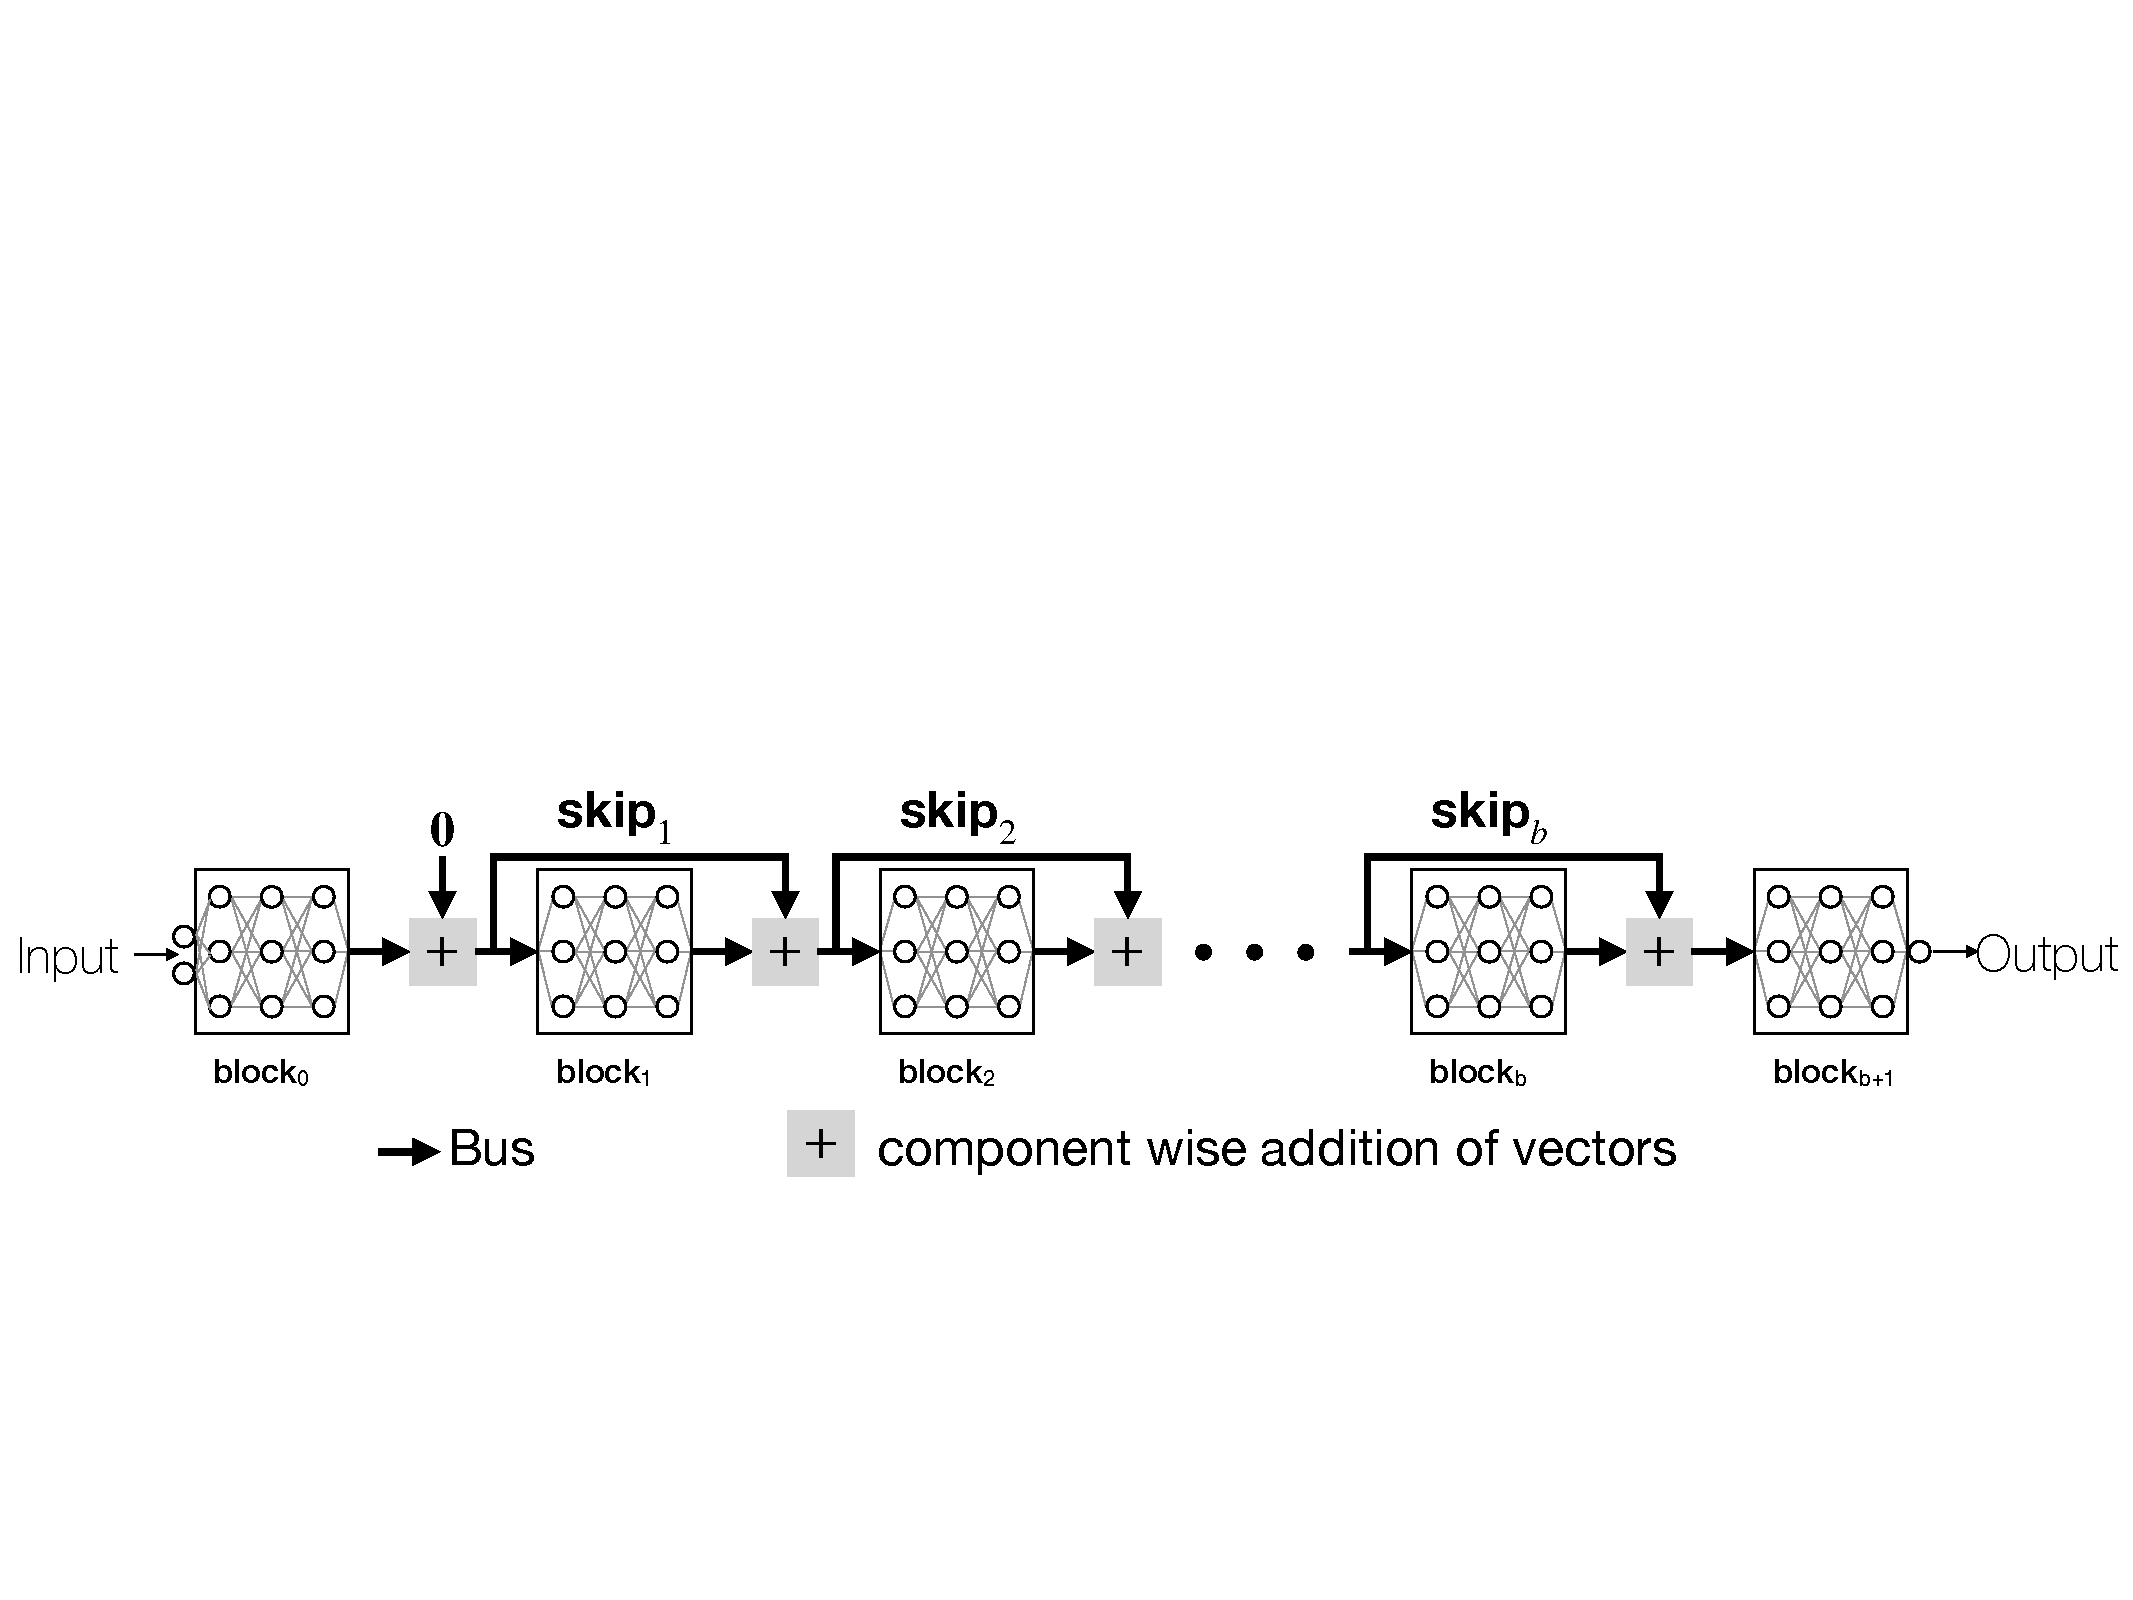
\includegraphics[scale=0.5]{figs/resnet.pdf}
}
\end{minipage}
\begin{minipage}{0.5\columnwidth}
\resizebox{\columnwidth}{!}{
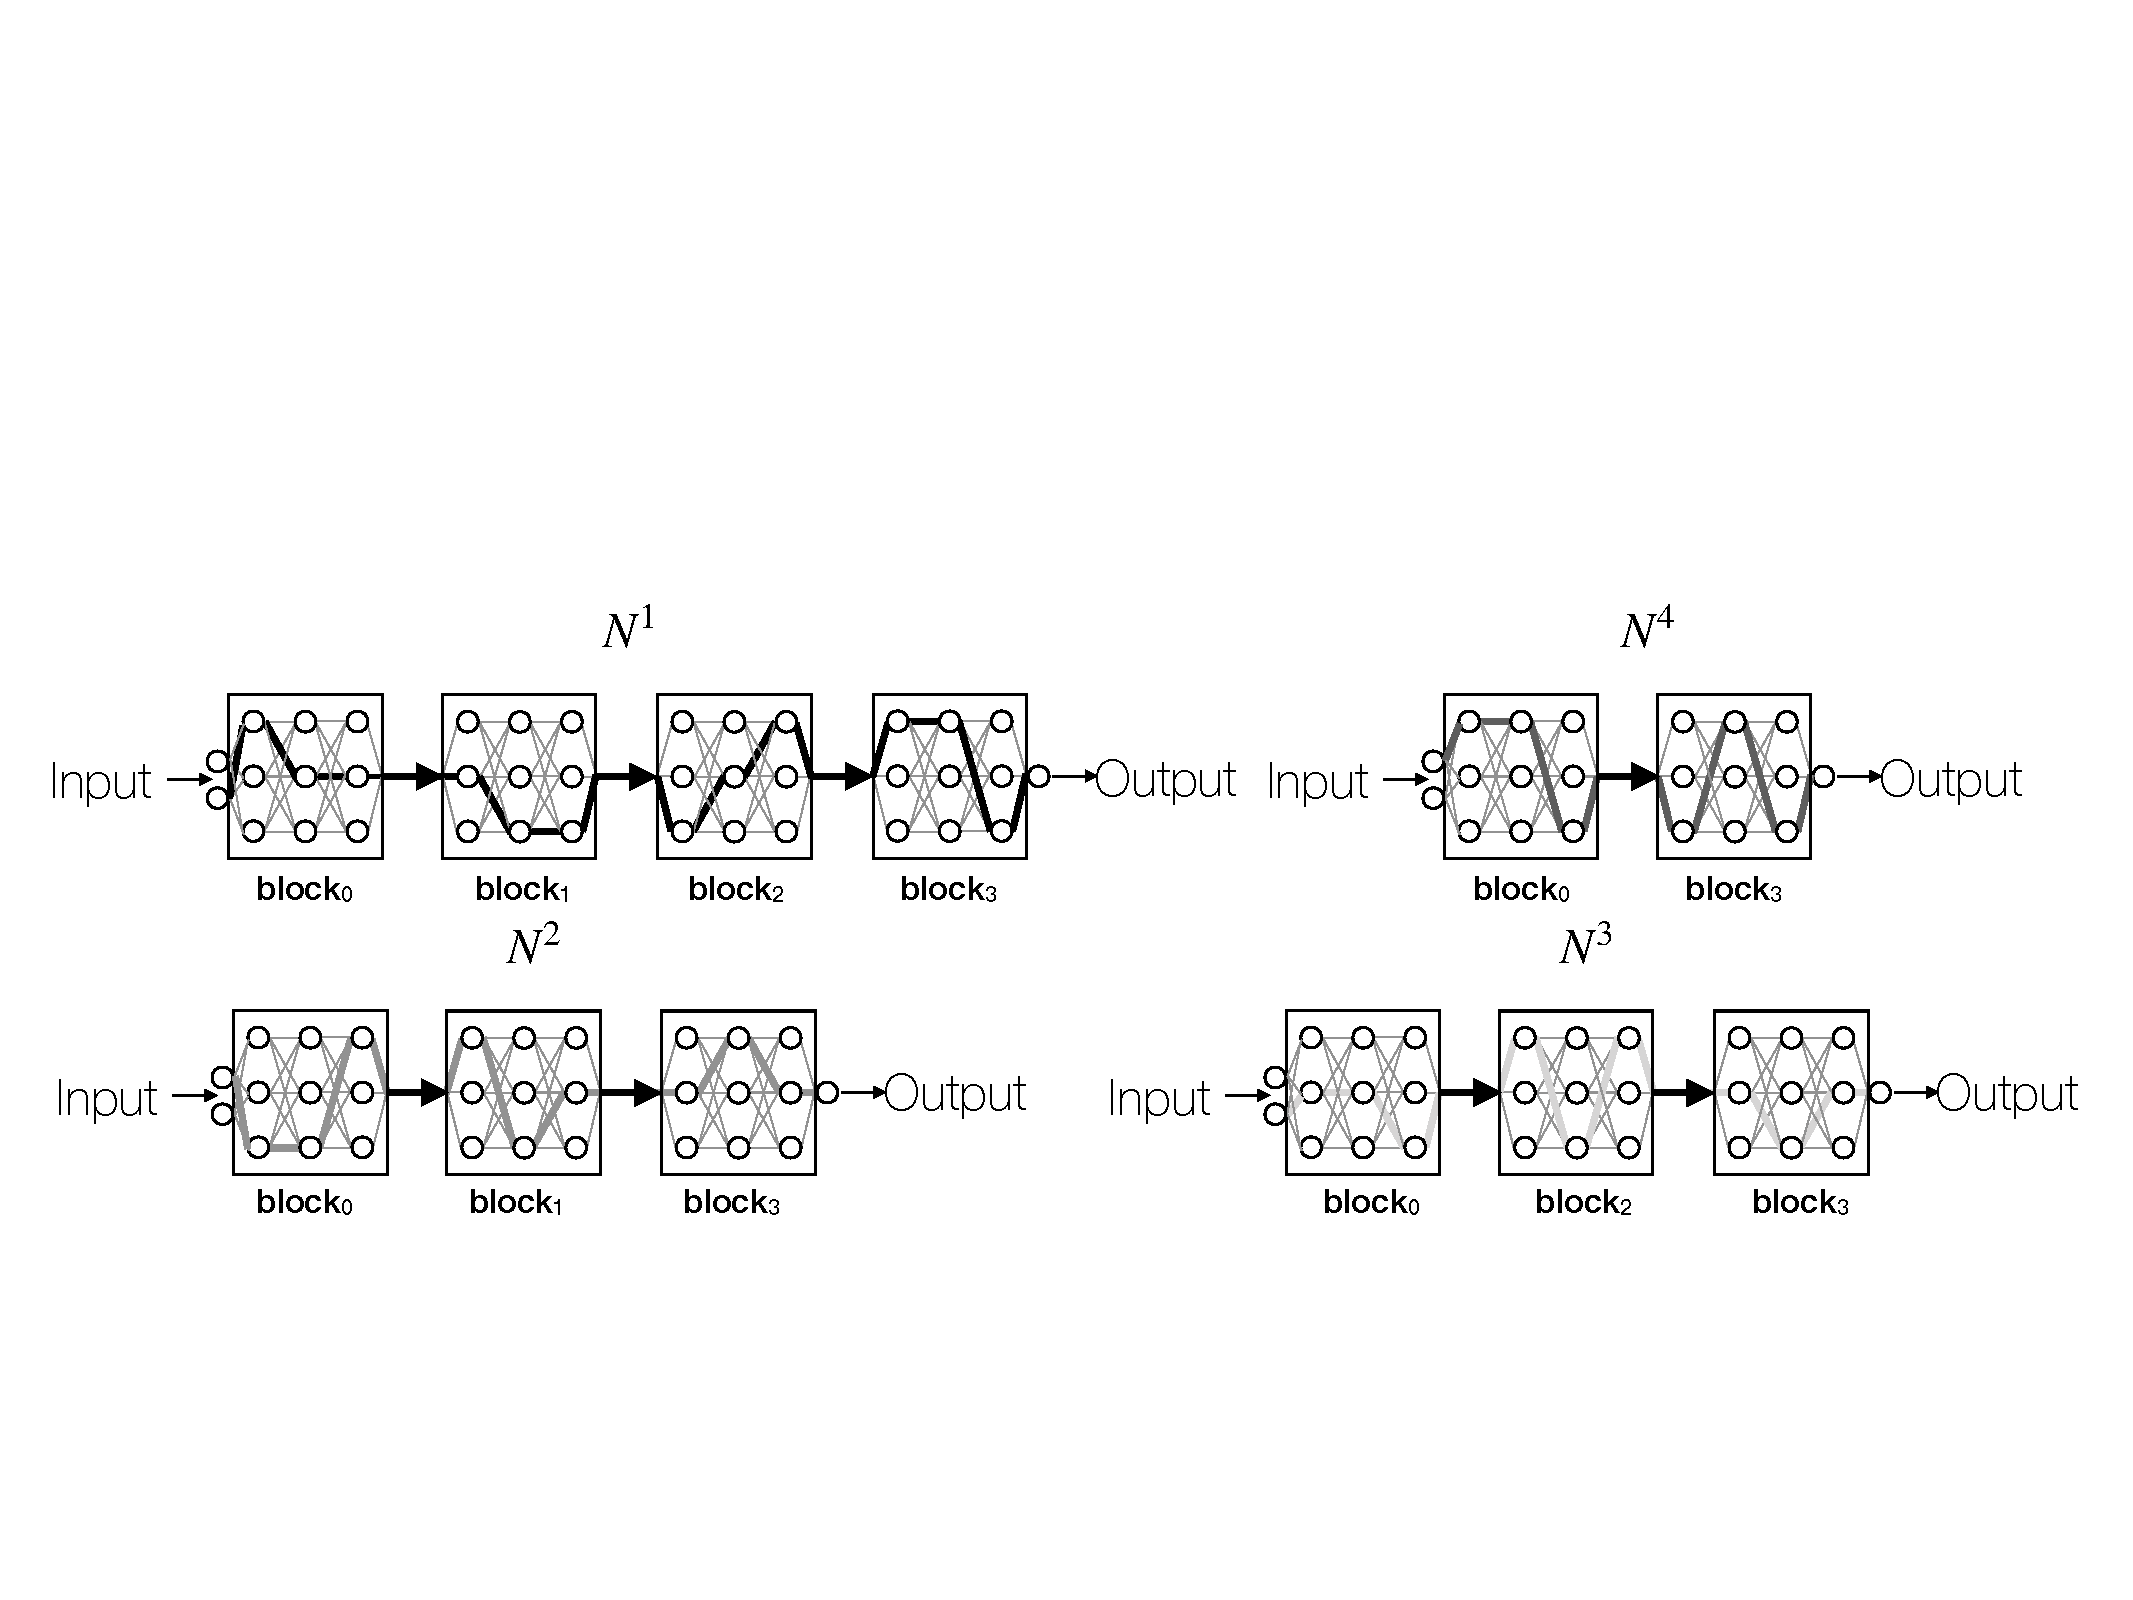
\includegraphics[scale=0.5]{figs/blocks.pdf}
}
\end{minipage}
\caption{\small{On the left is the ResNet with $b$ skip connections and $(b+2)$ blocks. On the right are the sub-FC networks $N^1$ obtained by skipping no blocks, $N^2$ and $N^4$ obtained by skipping block $1$ and $2$ respectively, and $N^3$ obtained by skipping both blocks $1$ and $2$.}}
\label{fig:resnet}
\end{figure}

\begin{definition}\label{def:subfcdnn}[Sub FC-DNNs]
Let $2^{[b]}$ denote the power set of $[b]$ and let $\J\in 2^{[b]}$ denote any subset of $[b]$. Define the`$\J^{th}$' sub-FC-DNN of the ResNet to be the fully connected network obtained by (i) including  $\text{block}_{j},\forall j\in \J$  and (ii) ignoring $\text{block}_{j},\forall j\notin \J$ (see \Cref{fig:resnet}).
\end{definition}
\begin{theorem}
[Sum of Product of Kernels Theorem]\label{th:res} Let $H^{\J}_{\Tf_0}$ be the NPK of the $\J^{th}$ sub-FC-DNN, and $\bfc^{\J}$ be the associated constant. Under \Cref{assmp:main}, we have:
\begin{align*}
\kv_{\Tdgn_0}\ra \sum_{\J\in 2^{[b]}}  \bfc^{\J} H^{\J}_{\Tf_0}, \,\, \text{as}\,\,  w\ra\infty
\end{align*}
\end{theorem}
\textbf{Note.} The sub-FC-DNNs we refer to in \Cref{th:mainres} belong to (or are parts of) the feature network from which the gates are obtained. 


\subsubsection{Discussion of Results}



%In order to completely address the `black box'-ness issue, an ideal goal is to aim for theoretical results (supported by empirical evidence) on finite time learning in finite width \texttt{DGN-NO-ACT}. We find this goal is too hard at this stage and do not pursue the same. The next level is to analyse  the primal linearity and the dual linearity separately. Understanding the primal linearity has two parts to it (i) `what do the learnt pre-activations mean?', and (ii) `how are useful pre-activations learnt?'. The `what' question is \emph{post-hoc}, i.e., we can inspect the learnt pre-activations after training. However, we believe that in order to obtain domain specific insights on what the learnt pre-activations mean, we might require domain specific tools. For instance, in the case of `image classification', the pre-activations are the result of series of convolutions by `filter banks', and in order to do full justice, any visual interpretation should also tally with the results from `filter bank' theory. We defer the `what' question for future work. We also believe new theory is required to answer `how are useful pre-activations learnt?', and defer the same to future work. In this paper,  


%$\bullet$ We empirically show that \texttt{DGN-NO-ACT} performs comparably well on standard datasets. 

%$\bullet$ We restate the prior result for the fully connected case so as to explicitise the role of gates, depth and width. We extend the dual view theory to cover  convolutions with global pooling and skip connections.  We show empirically that the value network learns path-by-path and not layer-by-layer.




%A \texttt{DGN-NO-ACT} learns the relation $\hat{y}(x)=\ip{\phi_\Tf(x),v_{\Tv}}$, by learning simultaneously the feature and value network parameters. The pre-activations generated by the feature network trigger the gates thereby directly dictating the neural path feature $\phi_\Tf(x)$. It was shown that neural path features (i.e., the gates) are learnt during training and such learning improves generalisation \cite{npk}. Thus, while the learning in feature network is key, we reserve its theoretical study for future work. In this section, we will analyse the dual linearity, wherein, the theoretical results are in the \emph{inifinite width regime} which yield us a \emph{kernel} interperation, using which we probe into the properties of finite width networks. In other words, our aim is not to propose pure kernel methods with the kernel derived from an inifnite width DNN. 

%For the purpose of analysing the dual, we first explicitise in \Cref{th:fc} an unnoticed invariance property in the prior result of \cite{npk} for fully connected networks. In \Cref{th:conv,th:res} we also extend the dual formulation to cover the cases of convolutions with global pooling and skip connections. These results justify the constant $\mathbf{1}$ input to the value network of the \texttt{DGN-NO-ACT}. We also experimentally verify the constant $\mathbf{1}$ input as well as destroying the layer-by-layer structure of the gates does not degrade the performance. While these results are surprising and counter intuitive with respect to the primal view, they are follow in a straightforward manner from the results in the dual view, thereby underscoring the fact the value network indeeed computes path-by-path, and eliminating the `mystery' as to whether sophisticated structures are learnt layer-by-layer.




\begin{comment}
\begin{figure}
\centering
\begin{minipage}{1.0\columnwidth}
\begin{minipage}{1.0\columnwidth}
\resizebox{0.99\columnwidth}{!}{
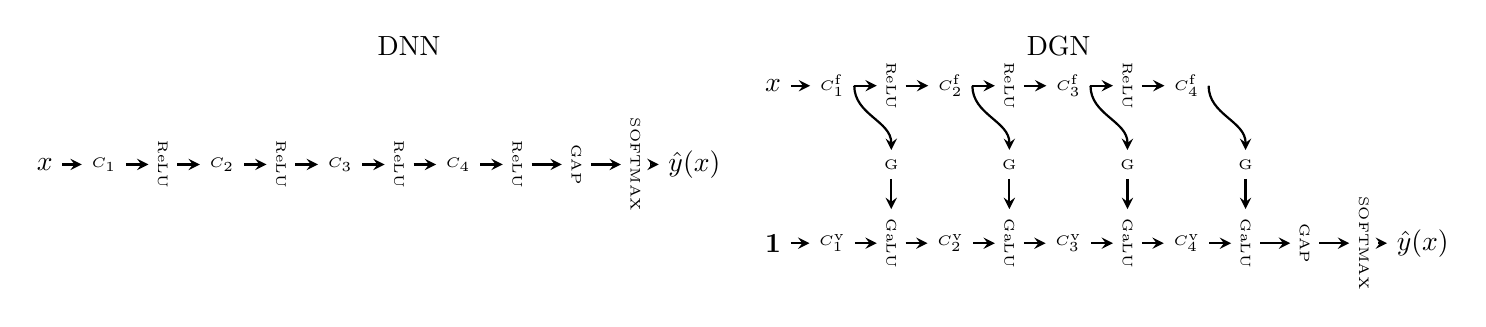
\begin{tikzpicture}
\node []  (dnn-text)at (-4.125,2) {DNN};

\node []  (dnn-output) at (-0.5,0.5) {$\hat{y}(x)$};
\node [rotate=-90]  (dnn-smax) at (-1.25,0.5) {\tiny{SOFTMAX}};
\draw [-stealth,thick]   (dnn-smax.north) -- (dnn-output.west);

\node [rotate=-90]  (dnn-gap) at (-2,0.5) {\tiny{GAP}};
\draw [-stealth,thick]   (dnn-gap.north) -- (dnn-smax.south);

\node [rotate=-90] (dnn-relu-4) at (-2.75,0.5){\tiny{ReLU}};
\node [] (dnn-c4) at (-3.5,0.5){\tiny{$C_4$}};
\draw [-stealth,thick]   (dnn-c4.east) -- (dnn-relu-4.south);
\draw [-stealth,thick]   (dnn-relu-4.north) -- (dnn-gap.south);



\node [rotate=-90] (dnn-relu-3) at (-4.25,0.5){\tiny{ReLU}};
\node [] (dnn-c3) at (-5,0.5){\tiny{$C_3$}};
\draw [-stealth,thick]   (dnn-c3.east) -- (dnn-relu-3.south);
\draw [-stealth,thick]   (dnn-relu-3.north) -- (dnn-c4.west);


\node [rotate=-90] (dnn-relu-2) at (-5.75,0.5){\tiny{ReLU}};
\node [] (dnn-c2) at (-6.5,0.5){\tiny{$C_2$}};
\draw [-stealth,thick]   (dnn-c2.east) -- (dnn-relu-2.south);
\draw [-stealth,thick]   (dnn-relu-2.north) -- (dnn-c3.west);

\node [rotate=-90] (dnn-relu-1) at (-7.25,0.5){\tiny{ReLU}};
\node [] (dnn-c1) at (-8,0.5){\tiny{$C_1$}};
\draw [-stealth,thick]   (dnn-c1.east) -- (dnn-relu-1.south);
\draw [-stealth,thick]   (dnn-relu-1.north) -- (dnn-c2.west);



\node [] (dnn-input) at (-8.75,0.5){$x$};
\draw [-stealth,thick]   (dnn-input.east) -- (dnn-c1.west);


%%%%%%%%%%%%%%%%%%%%%%%%%%%%%%%%%%%%%%%%%%%%%%%%%%%%%%%%%%%%%%%%%
\node []  (fntext)at (4.125,2) {DGN};

%\node []  (output) at (7.5,1.5) {$\hat{y}(x)$};


\node [] (dgn-f-c4) at (5.75,1.5){\tiny{$C^{\text{f}}_4$}};


\node [rotate=-90] (dgn-relu-3) at (5,1.5){\tiny{ReLU}};
\node [] (dgn-f-c3) at (4.25,1.5){\tiny{$C^{\text{f}}_3$}};
\draw [-stealth,thick]   (dgn-f-c3.east) -- (dgn-relu-3.south);
\draw [-stealth,thick]   (dgn-relu-3.north) -- (dgn-f-c4.west);


\node [rotate=-90] (dgn-relu-2) at (3.5,1.5){\tiny{ReLU}};
\node [] (dgn-f-c2) at (2.75,1.5){\tiny{$C^{\text{f}}_2$}};
\draw [-stealth,thick]   (dgn-f-c2.east) -- (dgn-relu-2.south);
\draw [-stealth,thick]   (dgn-relu-2.north) -- (dgn-f-c3.west);


\node [rotate=-90] (dgn-relu-1) at (2,1.5){\tiny{ReLU}};
\node [] (dgn-f-c1) at (1.25,1.5){\tiny{$C^{\text{f}}_1$}};
\draw [-stealth,thick]   (dgn-f-c1.east) -- (dgn-relu-1.south);
\draw [-stealth,thick]   (dgn-relu-1.north) -- (dgn-f-c2.west);



\node [] (dgn-f-input) at (0.5,1.5){$x$};
\draw [-stealth,thick]   (dgn-f-input.east) -- (dgn-f-c1.west);

\node []  (dgn-output) at (8.75,-0.5) {$\hat{y}(x)$};
\node [rotate=-90] (dgn-smax) at (8,-0.5){\tiny{SOFTMAX}};
\draw [-stealth,thick]   (dgn-smax.north)--(dgn-output.west);

\node [rotate=-90] (dgn-gap) at (7.25,-0.5){\tiny{GAP}};
\draw [-stealth,thick]   (dgn-gap.north)--(dgn-smax.south);



\node [rotate=-90] (dgn-galu-4) at (6.5,-0.5){\tiny{GaLU}};
\draw [-stealth,thick]   (dgn-galu-4.north) -- (dgn-gap.south);

\node [] (dgn-v-c4) at (5.75,-0.5){\tiny{$C^{\text{v}}_4$}};
\draw [-stealth,thick]   (dgn-v-c4.east) -- (dgn-galu-4.south);

\node [rotate=-90] (dgn-galu-3) at (5,-0.5){\tiny{GaLU}};
\node [] (dgn-v-c3) at (4.25,-0.5){\tiny{$C^{\text{v}}_3$}};
\draw [-stealth,thick]   (dgn-v-c3.east) -- (dgn-galu-3.south);
\draw [-stealth,thick]   (dgn-galu-3.north) -- (dgn-v-c4.west);



\node [rotate=-90] (dgn-galu-2) at (3.5,-0.5){\tiny{GaLU}};
\node [] (dgn-v-c2) at (2.75,-0.5){\tiny{$C^{\text{v}}_2$}};
\draw [-stealth,thick]   (dgn-v-c2.east) -- (dgn-galu-2.south);
\draw [-stealth,thick]   (dgn-galu-2.north) -- (dgn-v-c3.west);


\node [rotate=-90] (dgn-galu-1) at (2,-0.5){\tiny{GaLU}};
\node [] (dgn-v-c1) at (1.25,-0.5){\tiny{$C^{\text{v}}_1$}};

\draw [-stealth,thick]   (dgn-v-c1.east) -- (dgn-galu-1.south);
\draw [-stealth,thick]   (dgn-galu-1.north) -- (dgn-v-c2.west);




\node [] (dgn-input) at (0.5,-0.5){$\mathbf{1}$};
\draw [-stealth,thick]   (dgn-input.east) -- (dgn-v-c1.west);




\node[] (dgn-gating-1) at (2,0.5){\tiny{G}};
\draw [-stealth,thick]   (dgn-f-c1.east) to[out=-90,in=90] (dgn-gating-1.north);
\draw [-stealth,thick]   (dgn-gating-1.south) -- (dgn-galu-1.west);


\node[] (dgn-gating-2) at (3.5,0.5){\tiny{G}};
\draw [-stealth,thick]   (dgn-f-c2.east) to[out=-90,in=90] (dgn-gating-2.north);
\draw [-stealth,thick]   (dgn-gating-2.south) -- (dgn-galu-2.west);



\node[] (dgn-gating-3) at (5,0.5){\tiny{G}};
\draw [-stealth,thick]   (dgn-f-c3.east) to[out=-90,in=90] (dgn-gating-3.north);
\draw [-stealth,thick]   (dgn-gating-3.south) -- (dgn-galu-3.west);


\node[] (dgn-gating-4) at (6.5,0.5){\tiny{G}};
\draw [-stealth,thick]   (dgn-f-c4.east) to[out=-90,in=90] (dgn-gating-4.north);
\draw [-stealth,thick]   (dgn-gating-4.south) -- (dgn-galu-4.west);

	
\end{tikzpicture}


}
\end{minipage}
\begin{minipage}{1.0\columnwidth}
\resizebox{0.99\columnwidth}{!}{
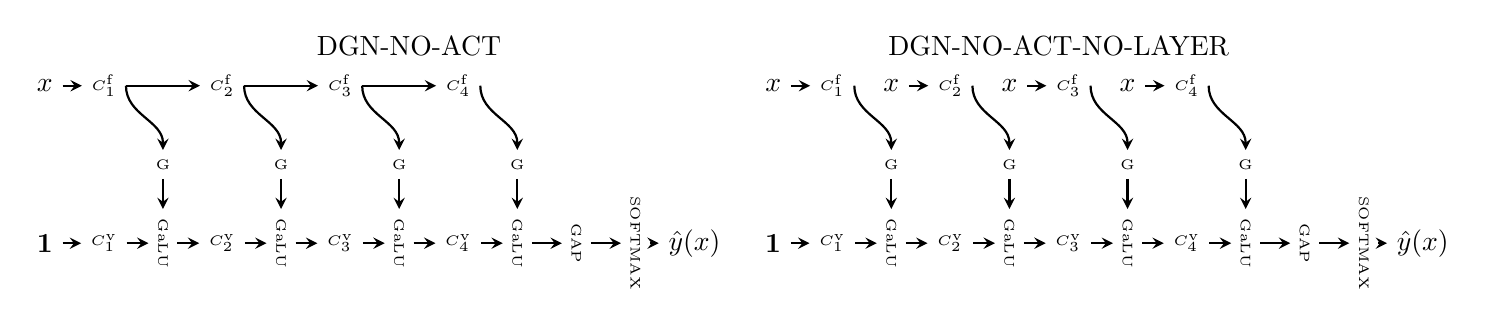
\begin{tikzpicture}
\node []  (fntext)at (-4.125,2) {DGN-NO-ACT};

%\node []  (output) at (7.5,1.5) {$\hat{y}(x)$};


\node [] (dgn1-f-c4) at (-3.5,1.5){\tiny{$C^{\text{f}}_4$}};
\node [] (dgn1-f-c3) at (-5,1.5){\tiny{$C^{\text{f}}_3$}};
\node [] (dgn1-f-c2) at (-6.5,1.5){\tiny{$C^{\text{f}}_2$}};
\node [] (dgn1-f-c1) at (-8,1.5){\tiny{$C^{\text{f}}_1$}};
\node [] (dgn1-input-f) at (-8.75,1.5){$x$};
\draw [-stealth,thick]   (dgn1-f-c3.east) -- (dgn1-f-c4.west);
\draw [-stealth,thick]   (dgn1-f-c2.east) -- (dgn1-f-c3.west);
\draw [-stealth,thick]   (dgn1-f-c1.east) -- (dgn1-f-c2.west);
\draw [-stealth,thick]   (dgn1-input-f.east) -- (dgn1-f-c1.west);



\node []  (dgn1-output) at (-0.5,-0.5) {$\hat{y}(x)$};

\node [rotate=-90] (dgn1-smax) at (-1.25,-0.5){\tiny{SOFTMAX}};
\draw [-stealth,thick]   (dgn1-smax.north)--(dgn1-output.west);

\node [rotate=-90] (dgn1-gap) at (-2,-0.5){\tiny{GAP}};
\draw [-stealth,thick]   (dgn1-gap.north)--(dgn1-smax.south);


\node [rotate=-90] (dgn1-galu-4) at (-2.75,-0.5){\tiny{GaLU}};
\draw [-stealth,thick]   (dgn1-galu-4.north)--(dgn1-gap.south);

\node [] (dgn1-v-c4) at (-3.5,-0.5){\tiny{$C^{\text{v}}_4$}};
\draw [-stealth,thick]   (dgn1-v-c4.east) -- (dgn1-galu-4.south);


\node [rotate=-90] (dgn1-galu-3) at (-4.25,-0.5){\tiny{GaLU}};
\draw [-stealth,thick]   (dgn1-galu-3.north) -- (dgn1-v-c4.west);

\node [] (dgn1-v-c3) at (-5,-0.5){\tiny{$C^{\text{v}}_3$}};
\draw [-stealth,thick]   (dgn1-v-c3.east) -- (dgn1-galu-3.south);


\node [rotate=-90] (dgn1-galu-2) at (-5.75,-0.5){\tiny{GaLU}};
\draw [-stealth,thick]   (dgn1-galu-2.north) -- (dgn1-v-c3.west);

\node [] (dgn1-v-c2) at (-6.5,-0.5){\tiny{$C^{\text{v}}_2$}};
\draw [-stealth,thick]   (dgn1-v-c2.east) -- (dgn1-galu-2.south);


\node [rotate=-90] (dgn1-galu-1) at (-7.25,-0.5){\tiny{GaLU}};
\draw [-stealth,thick]   (dgn1-galu-1.north) -- (dgn1-v-c2.west);


\node [] (dgn1-v-c1) at (-8,-0.5){\tiny{$C^{\text{v}}_1$}};
\draw [-stealth,thick]   (dgn1-v-c1.east) -- (dgn1-galu-1.south);


\node [] (dgn1-v-input) at (-8.75,-0.5){$\mathbf{1}$};




\node[] (dgn1-gating-4) at (-2.75,0.5){\tiny{G}};
\node[] (dgn1-gating-3) at (-4.25,0.5){\tiny{G}};
\node[] (dgn1-gating-2) at (-5.75,0.5){\tiny{G}};
\node[] (dgn1-gating-1) at (-7.25,0.5){\tiny{G}};

\draw [-stealth,thick]   (dgn1-f-c1.east) to[out=-90,in=90] (dgn1-gating-1.north);
\draw [-stealth,thick]   (dgn1-gating-1.south) -- (dgn1-galu-1.west);



\draw [-stealth,thick]   (dgn1-f-c2.east) to[out=-90,in=90] (dgn1-gating-2.north);
\draw [-stealth,thick]   (dgn1-gating-2.south) -- (dgn1-galu-2.west);




\draw [-stealth,thick]   (dgn1-f-c3.east) to[out=-90,in=90] (dgn1-gating-3.north);
\draw [-stealth,thick]   (dgn1-gating-3.south) -- (dgn1-galu-3.west);



\draw [-stealth,thick]   (dgn1-f-c4.east) to[out=-90,in=90] (dgn1-gating-4.north);
\draw [-stealth,thick]   (dgn1-gating-4.south) -- (dgn1-galu-4.west);

\draw [-stealth,thick]   (dgn1-v-input.east) -- (dgn1-v-c1.west);

%%%%%%%%%%%%%%%%%%%%%%%%%%%%%%%%%%%%%%%%%%%%%%%%%%%%%%%%%%%%%%%%%
\node []  (fntext)at (4.125,2) {DGN-NO-ACT-NO-LAYER};

%\node []  (output) at (7.5,1.5) {$\hat{y}(x)$};

\node [] (dgn-f-input) at (0.5,1.5){$x$};
\node [] (dgn-f-c4) at (5.75,1.5){\tiny{$C^{\text{f}}_4$}};

\node [] (dgn-f-x-4) at (5,1.5){$x$};


\node [] (dgn-f-c3) at (4.25,1.5){\tiny{$C^{\text{f}}_3$}};
\node [] (dgn-f-x-3) at (3.5,1.5){$x$};

\node [] (dgn-f-c2) at (2.75,1.5){\tiny{$C^{\text{f}}_2$}};
\node [] (dgn-f-x-2) at (2,1.5){$x$};

\node [] (dgn-f-c1) at (1.25,1.5){\tiny{$C^{\text{f}}_1$}};

\draw [-stealth,thick]   (dgn-f-input.east) -- (dgn-f-c1.west);
\draw [-stealth,thick]   (dgn-f-x-2.east) -- (dgn-f-c2.west);
\draw [-stealth,thick]   (dgn-f-x-3.east) -- (dgn-f-c3.west);
\draw [-stealth,thick]   (dgn-f-x-4.east) -- (dgn-f-c4.west);


\node []  (dgn-output) at (8.75,-0.5) {$\hat{y}(x)$};



\node [rotate=-90] (dgn-smax) at (8,-0.5){\tiny{SOFTMAX}};
\draw [-stealth,thick]   (dgn-smax.north) -- (dgn-output.west);
;
\node [rotate=-90] (dgn-gap) at (7.25,-0.5){\tiny{GAP}};
\draw [-stealth,thick]   (dgn-gap.north) -- (dgn-smax.south);



\node [rotate=-90] (dgn-galu-4) at (6.5,-0.5){\tiny{GaLU}};

\draw [-stealth,thick]   (dgn-galu-4.north) -- (dgn-gap.south);
\node [] (dgn-v-c4) at (5.75,-0.5){\tiny{$C^{\text{v}}_4$}};
\draw [-stealth,thick]   (dgn-v-c4.east) -- (dgn-galu-4.south);


\node [rotate=-90] (dgn-galu-3) at (5,-0.5){\tiny{GaLU}};
\draw [-stealth,thick]   (dgn-galu-3.north) -- (dgn-v-c4.west);


\node [] (dgn-v-c3) at (4.25,-0.5){\tiny{$C^{\text{v}}_3$}};
\draw [-stealth,thick]   (dgn-v-c3.east) -- (dgn-galu-3.south);


\node [rotate=-90] (dgn-galu-2) at (3.5,-0.5){\tiny{GaLU}};
\draw [-stealth,thick]   (dgn-galu-2.north) -- (dgn-v-c3.west);

\node [] (dgn-v-c2) at (2.75,-0.5){\tiny{$C^{\text{v}}_2$}};
\draw [-stealth,thick]   (dgn-v-c2.east) -- (dgn-galu-2.south);


\node [rotate=-90] (dgn-galu-1) at (2.0,-0.5){\tiny{GaLU}};
\draw [-stealth,thick]   (dgn-galu-1.north) -- (dgn-v-c2.west);

\node [] (dgn-v-c1) at (1.25,-0.5){\tiny{$C^{\text{v}}_1$}};
\draw [-stealth,thick]   (dgn-v-c1.east) -- (dgn-galu-1.south);


\node [] (dgn-v-input) at (0.5,-0.5){$\mathbf{1}$};


\node[] (dgn-gating-1) at (2.0,0.5){\tiny{G}};
\draw [-stealth,thick]   (dgn-f-c1.east) to[out=-90,in=90] (dgn-gating-1.north);
\draw [-stealth,thick]   (dgn-gating-1.south) -- (dgn-galu-1.west);


\node[] (dgn-gating-2) at (3.5,0.5){\tiny{G}};
\draw [-stealth,thick]   (dgn-f-c2.east) to[out=-90,in=90] (dgn-gating-2.north);
\draw [-stealth,thick]   (dgn-gating-2.south) -- (dgn-galu-2.west);



\node[] (dgn-gating-3) at (5,0.5){\tiny{G}};
\draw [-stealth,thick]   (dgn-f-c3.east) to[out=-90,in=90] (dgn-gating-3.north);
\draw [-stealth,thick]   (dgn-gating-3.south) -- (dgn-galu-3.west);


\node[] (dgn-gating-4) at (6.5,0.5){\tiny{G}};
\draw [-stealth,thick]   (dgn-f-c4.east) to[out=-90,in=90] (dgn-gating-4.north);
\draw [-stealth,thick]   (dgn-gating-4.south) -- (dgn-galu-4.west);

\draw [-stealth,thick]   (dgn-v-input.east) -- (dgn-v-c1.west);
	
\end{tikzpicture}


}
\end{minipage}
\end{minipage}
\caption{$4$ convolutional layers with GAP}
\label{fig:c4gap}
\end{figure}
\end{comment}

%\section{DLGN:  Disentangling the computation in DNNs with ReLUs}\label{sec:dlgn}
\begin{figure}[!b]
\centering
\begin{minipage}{0.40\columnwidth}
\centering
\resizebox{0.99\columnwidth}{!}{
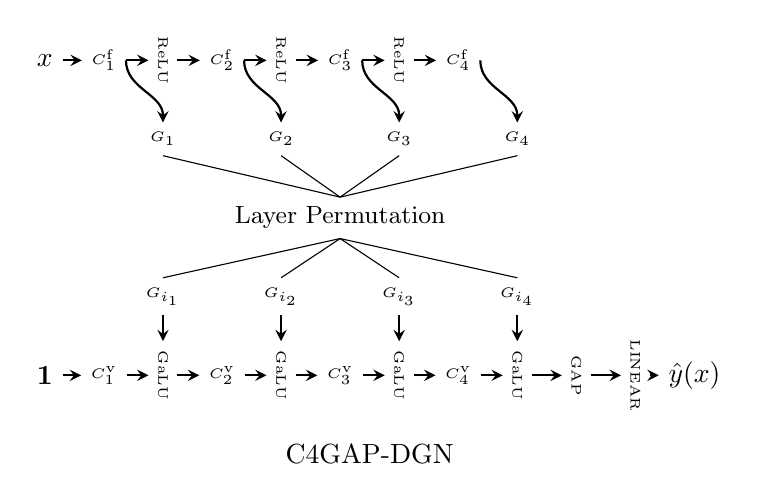
\begin{tikzpicture}
%%%%%%%%%%%%%%%%%%%%%%%%%%%%%%%%%%%%%%%%%%%%%%%%%%%%%%%%%%%%%%%%%
\node []  (fntext)at (4.625,-3.5) {C4GAP-DGN};

%\node []  (output) at (7.5,1.5) {$\hat{y}(x)$};


\node [] (dgn-f-c4) at (5.75,1.5){\tiny{$C^{\text{f}}_4$}};


\node [rotate=-90] (dgn-relu-3) at (5,1.5){\tiny{ReLU}};
\node [] (dgn-f-c3) at (4.25,1.5){\tiny{$C^{\text{f}}_3$}};
\draw [-stealth,thick]   (dgn-f-c3.east) -- (dgn-relu-3.south);
\draw [-stealth,thick]   (dgn-relu-3.north) -- (dgn-f-c4.west);


\node [rotate=-90] (dgn-relu-2) at (3.5,1.5){\tiny{ReLU}};
\node [] (dgn-f-c2) at (2.75,1.5){\tiny{$C^{\text{f}}_2$}};
\draw [-stealth,thick]   (dgn-f-c2.east) -- (dgn-relu-2.south);
\draw [-stealth,thick]   (dgn-relu-2.north) -- (dgn-f-c3.west);


\node [rotate=-90] (dgn-relu-1) at (2,1.5){\tiny{ReLU}};
\node [] (dgn-f-c1) at (1.25,1.5){\tiny{$C^{\text{f}}_1$}};
\draw [-stealth,thick]   (dgn-f-c1.east) -- (dgn-relu-1.south);
\draw [-stealth,thick]   (dgn-relu-1.north) -- (dgn-f-c2.west);



\node [] (dgn-f-input) at (0.5,1.5){$x$};
\draw [-stealth,thick]   (dgn-f-input.east) -- (dgn-f-c1.west);




\node []  (dgn-output) at (8.75,-2.5) {$\hat{y}(x)$};
\node [rotate=-90] (dgn-smax) at (8,-2.5){\tiny{LINEAR}};
\draw [-stealth,thick]   (dgn-smax.north)--(dgn-output.west);

\node [rotate=-90] (dgn-gap) at (7.25,-2.5){\tiny{GAP}};
\draw [-stealth,thick]   (dgn-gap.north)--(dgn-smax.south);



\node [rotate=-90] (dgn-galu-4) at (6.5,-2.5){\tiny{GaLU}};
\draw [-stealth,thick]   (dgn-galu-4.north) -- (dgn-gap.south);

\node [] (dgn-v-c4) at (5.75,-2.5){\tiny{$C^{\text{v}}_4$}};
\draw [-stealth,thick]   (dgn-v-c4.east) -- (dgn-galu-4.south);

\node [rotate=-90] (dgn-galu-3) at (5,-2.5){\tiny{GaLU}};
\node [] (dgn-v-c3) at (4.25,-2.5){\tiny{$C^{\text{v}}_3$}};
\draw [-stealth,thick]   (dgn-v-c3.east) -- (dgn-galu-3.south);
\draw [-stealth,thick]   (dgn-galu-3.north) -- (dgn-v-c4.west);



\node [rotate=-90] (dgn-galu-2) at (3.5,-2.5){\tiny{GaLU}};
\node [] (dgn-v-c2) at (2.75,-2.5){\tiny{$C^{\text{v}}_2$}};
\draw [-stealth,thick]   (dgn-v-c2.east) -- (dgn-galu-2.south);
\draw [-stealth,thick]   (dgn-galu-2.north) -- (dgn-v-c3.west);


\node [rotate=-90] (dgn-galu-1) at (2,-2.5){\tiny{GaLU}};
\node [] (dgn-v-c1) at (1.25,-2.5){\tiny{$C^{\text{v}}_1$}};

\draw [-stealth,thick]   (dgn-v-c1.east) -- (dgn-galu-1.south);
\draw [-stealth,thick]   (dgn-galu-1.north) -- (dgn-v-c2.west);




\node [] (dgn-input) at (0.5,-2.5){$\mathbf{1}$};
\draw [-stealth,thick]   (dgn-input.east) -- (dgn-v-c1.west);


\node[] (dgn-gating-1-up) at (2,0.5){\tiny{$G_{1}$}};
\draw [-stealth,thick]   (dgn-f-c1.east) to[out=-90,in=90] (dgn-gating-1-up.north);


\node[] (dgn-gating-2-up) at (3.5,0.5){\tiny{$G_{2}$}};
\draw [-stealth,thick]   (dgn-f-c2.east) to[out=-90,in=90] (dgn-gating-2-up.north);



\node[] (dgn-gating-3-up) at (5,0.5){\tiny{$G_{3}$}};
\draw [-stealth,thick]   (dgn-f-c3.east) to[out=-90,in=90] (dgn-gating-3-up.north);


\node[] (dgn-gating-4-up) at (6.5,0.5){\tiny{$G_{4}$}};
\draw [-stealth,thick]   (dgn-f-c4.east) to[out=-90,in=90] (dgn-gating-4-up.north);





\node[] (dgn-gating-1) at (2,-1.5){\tiny{$G_{i_1}$}};
\draw [-stealth,thick]   (dgn-gating-1.south) -- (dgn-galu-1.west);


\node[] (dgn-gating-2) at (3.5,-1.5){\tiny{$G_{i_2}$}};
\draw [-stealth,thick]   (dgn-gating-2.south) -- (dgn-galu-2.west);



\node[] (dgn-gating-3) at (5,-1.5){\tiny{$G_{i_3}$}};
\draw [-stealth,thick]   (dgn-gating-3.south) -- (dgn-galu-3.west);


\node[] (dgn-gating-4) at (6.5,-1.5){\tiny{$G_{i_4}$}};
\draw [-stealth,thick]   (dgn-gating-4.south) -- (dgn-galu-4.west);



\node[] (permutation) at (4.25,-0.5){\small{Layer Permutation}};

\draw [-]   (dgn-gating-1-up.south) -- (permutation.north);
\draw [-]   (dgn-gating-4-up.south) -- (permutation.north);
\draw [-]   (dgn-gating-2-up.south) -- (permutation.north);
\draw [-]   (dgn-gating-3-up.south) -- (permutation.north);



\draw [-]  (permutation.south) --  (dgn-gating-1.north)  ;
\draw [-]  (permutation.south) --  (dgn-gating-2.north)  ;
\draw [-]  (permutation.south) --  (dgn-gating-3.north)  ;
\draw [-]  (permutation.south) --  (dgn-gating-4.north)  ;

	
\end{tikzpicture}


}
\end{minipage}
\begin{minipage}{0.40\columnwidth}
\centering
\resizebox{0.99\columnwidth}{!}{
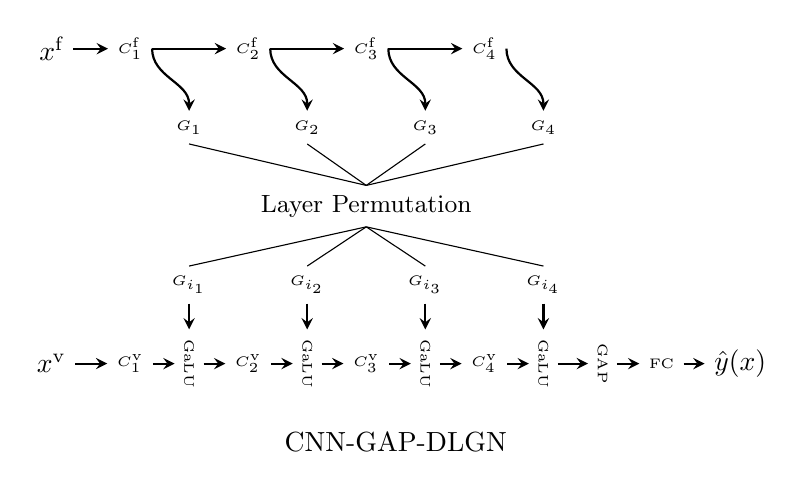
\begin{tikzpicture}
\node []  (fntext)at (-4.625,-3.5) {CNN-GAP-DLGN};

%\node []  (output) at (7.5,1.5) {$\hat{y}(x)$};


\node [] (dgn1-f-c4) at (-3.5,1.5){\tiny{$C^{\text{f}}_4$}};
\node [] (dgn1-f-c3) at (-5,1.5){\tiny{$C^{\text{f}}_3$}};
\node [] (dgn1-f-c2) at (-6.5,1.5){\tiny{$C^{\text{f}}_2$}};
\node [] (dgn1-f-c1) at (-8,1.5){\tiny{$C^{\text{f}}_1$}};
\node [] (dgn1-input-f) at (-9,1.5){$x^{\text{f}}$};
\draw [-stealth,thick]   (dgn1-f-c3.east) -- (dgn1-f-c4.west);
\draw [-stealth,thick]   (dgn1-f-c2.east) -- (dgn1-f-c3.west);
\draw [-stealth,thick]   (dgn1-f-c1.east) -- (dgn1-f-c2.west);
\draw [-stealth,thick]   (dgn1-input-f.east) -- (dgn1-f-c1.west);



\node []  (dgn1-output) at (-0.25,-2.5) {$\hat{y}(x)$};

\node [] (dgn1-smax) at (-1.25,-2.5){\tiny{FC}};
\draw [-stealth,thick]   (dgn1-smax.east)--(dgn1-output.west);

\node [rotate=-90] (dgn1-gap) at (-2,-2.5){\tiny{GAP}};
\draw [-stealth,thick]   (dgn1-gap.north)--(dgn1-smax.west);


\node [rotate=-90] (dgn1-galu-4) at (-2.75,-2.5){\tiny{GaLU}};
\draw [-stealth,thick]   (dgn1-galu-4.north)--(dgn1-gap.south);

\node [] (dgn1-v-c4) at (-3.5,-2.5){\tiny{$C^{\text{v}}_4$}};
\draw [-stealth,thick]   (dgn1-v-c4.east) -- (dgn1-galu-4.south);


\node [rotate=-90] (dgn1-galu-3) at (-4.25,-2.5){\tiny{GaLU}};
\draw [-stealth,thick]   (dgn1-galu-3.north) -- (dgn1-v-c4.west);

\node [] (dgn1-v-c3) at (-5,-2.5){\tiny{$C^{\text{v}}_3$}};
\draw [-stealth,thick]   (dgn1-v-c3.east) -- (dgn1-galu-3.south);


\node [rotate=-90] (dgn1-galu-2) at (-5.75,-2.5){\tiny{GaLU}};
\draw [-stealth,thick]   (dgn1-galu-2.north) -- (dgn1-v-c3.west);

\node [] (dgn1-v-c2) at (-6.5,-2.5){\tiny{$C^{\text{v}}_2$}};
\draw [-stealth,thick]   (dgn1-v-c2.east) -- (dgn1-galu-2.south);


\node [rotate=-90] (dgn1-galu-1) at (-7.25,-2.5){\tiny{GaLU}};
\draw [-stealth,thick]   (dgn1-galu-1.north) -- (dgn1-v-c2.west);


\node [] (dgn1-v-c1) at (-8,-2.5){\tiny{$C^{\text{v}}_1$}};
\draw [-stealth,thick]   (dgn1-v-c1.east) -- (dgn1-galu-1.south);


\node [] (dgn1-v-input) at (-9,-2.5){$x^{\text{v}}$};

\draw [-stealth,thick]   (dgn1-v-input.east) -- (dgn1-v-c1.west);


\node[] (dgn1-gating-4-up) at (-2.75,0.5){\tiny{$G_{4}$}};
\draw [-stealth,thick]   (dgn1-f-c4.east) to[out=-90,in=90] (dgn1-gating-4-up.north);


\node[] (dgn1-gating-3-up) at (-4.25,0.5){\tiny{$G_{3}$}};
\draw [-stealth,thick]   (dgn1-f-c3.east) to[out=-90,in=90] (dgn1-gating-3-up.north);



\node[] (dgn1-gating-2-up) at (-5.75,0.5){\tiny{$G_{2}$}};
\draw [-stealth,thick]   (dgn1-f-c2.east) to[out=-90,in=90] (dgn1-gating-2-up.north);


\node[] (dgn1-gating-1-up) at (-7.25,0.5){\tiny{$G_{1}$}};
\draw [-stealth,thick]   (dgn1-f-c1.east) to[out=-90,in=90] (dgn1-gating-1-up.north);





\node[] (dgn1-gating-4) at (-2.75,-1.5){\tiny{$G_{i_4}$}};
\draw [-stealth,thick]   (dgn1-gating-4.south) -- (dgn1-galu-4.west);


\node[] (dgn1-gating-3) at (-4.25,-1.5){\tiny{$G_{i_3}$}};
\draw [-stealth,thick]   (dgn1-gating-3.south) -- (dgn1-galu-3.west);



\node[] (dgn1-gating-2) at (-5.75,-1.5){\tiny{$G_{i_2}$}};
\draw [-stealth,thick]   (dgn1-gating-2.south) -- (dgn1-galu-2.west);


\node[] (dgn1-gating-1) at (-7.25,-1.5){\tiny{$G_{i_1}$}};
\draw [-stealth,thick]   (dgn1-gating-1.south) -- (dgn1-galu-1.west);



\node[] (permutation1) at (-5,-0.5){\small{Layer Permutation}};

\draw [-]   (dgn1-gating-1-up.south) -- (permutation1.north);
\draw [-]   (dgn1-gating-4-up.south) -- (permutation1.north);
\draw [-]   (dgn1-gating-2-up.south) -- (permutation1.north);
\draw [-]   (dgn1-gating-3-up.south) -- (permutation1.north);



\draw [-]  (permutation1.south) --  (dgn1-gating-1.north)  ;
\draw [-]  (permutation1.south) --  (dgn1-gating-2.north)  ;
\draw [-]  (permutation1.south) --  (dgn1-gating-3.north)  ;
\draw [-]  (permutation1.south) --  (dgn1-gating-4.north)  ;


%%%%%%%%%%%%%%%%%%%%%%%%%%%%%%%%%%%%%%%%%%%%%%%%%%%%%%%%%%%%%%%%%
	
\end{tikzpicture}


}
\end{minipage}
%\begin{minipage}{0.30\columnwidth}
%\centering
%\resizebox{0.99\columnwidth}{!}{
%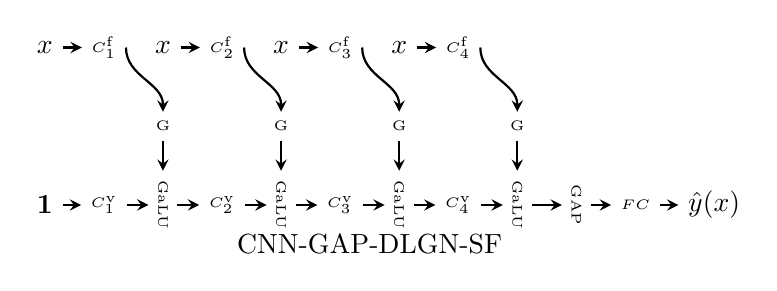
\begin{tikzpicture}
%%%%%%%%%%%%%%%%%%%%%%%%%%%%%%%%%%%%%%%%%%%%%%%%%%%%%%%%%%%%%%%%%
\node []  (fntext)at (4.625,-1) {CNN-GAP-DLGN-SF};

%\node []  (output) at (7.5,1.5) {$\hat{y}(x)$};

\node [] (dgn-f-input) at (0.5,1.5){$x$};
\node [] (dgn-f-c4) at (5.75,1.5){\tiny{$C^{\text{f}}_4$}};

\node [] (dgn-f-x-4) at (5,1.5){$x$};


\node [] (dgn-f-c3) at (4.25,1.5){\tiny{$C^{\text{f}}_3$}};
\node [] (dgn-f-x-3) at (3.5,1.5){$x$};

\node [] (dgn-f-c2) at (2.75,1.5){\tiny{$C^{\text{f}}_2$}};
\node [] (dgn-f-x-2) at (2,1.5){$x$};

\node [] (dgn-f-c1) at (1.25,1.5){\tiny{$C^{\text{f}}_1$}};

\draw [-stealth,thick]   (dgn-f-input.east) -- (dgn-f-c1.west);
\draw [-stealth,thick]   (dgn-f-x-2.east) -- (dgn-f-c2.west);
\draw [-stealth,thick]   (dgn-f-x-3.east) -- (dgn-f-c3.west);
\draw [-stealth,thick]   (dgn-f-x-4.east) -- (dgn-f-c4.west);


\node []  (dgn-output) at (9,-0.5) {$\hat{y}(x)$};



\node [] (dgn-smax) at (8,-0.5){\tiny{$FC$}};
\draw [-stealth,thick]   (dgn-smax.east) -- (dgn-output.west);
;
\node [rotate=-90] (dgn-gap) at (7.25,-0.5){\tiny{GAP}};
\draw [-stealth,thick]   (dgn-gap.north) -- (dgn-smax.west);



\node [rotate=-90] (dgn-galu-4) at (6.5,-0.5){\tiny{GaLU}};

\draw [-stealth,thick]   (dgn-galu-4.north) -- (dgn-gap.south);
\node [] (dgn-v-c4) at (5.75,-0.5){\tiny{$C^{\text{v}}_4$}};
\draw [-stealth,thick]   (dgn-v-c4.east) -- (dgn-galu-4.south);


\node [rotate=-90] (dgn-galu-3) at (5,-0.5){\tiny{GaLU}};
\draw [-stealth,thick]   (dgn-galu-3.north) -- (dgn-v-c4.west);


\node [] (dgn-v-c3) at (4.25,-0.5){\tiny{$C^{\text{v}}_3$}};
\draw [-stealth,thick]   (dgn-v-c3.east) -- (dgn-galu-3.south);


\node [rotate=-90] (dgn-galu-2) at (3.5,-0.5){\tiny{GaLU}};
\draw [-stealth,thick]   (dgn-galu-2.north) -- (dgn-v-c3.west);

\node [] (dgn-v-c2) at (2.75,-0.5){\tiny{$C^{\text{v}}_2$}};
\draw [-stealth,thick]   (dgn-v-c2.east) -- (dgn-galu-2.south);


\node [rotate=-90] (dgn-galu-1) at (2.0,-0.5){\tiny{GaLU}};
\draw [-stealth,thick]   (dgn-galu-1.north) -- (dgn-v-c2.west);

\node [] (dgn-v-c1) at (1.25,-0.5){\tiny{$C^{\text{v}}_1$}};
\draw [-stealth,thick]   (dgn-v-c1.east) -- (dgn-galu-1.south);


\node [] (dgn-v-input) at (0.5,-0.5){$\mathbf{1}$};

\draw [-stealth,thick]   (dgn-v-input.east) -- (dgn-v-c1.west);


\node[] (dgn-gating-1) at (2,0.5){\tiny{G}};
\draw [-stealth,thick]   (dgn-f-c1.east) to[out=-90,in=90] (dgn-gating-1.north);


\node[] (dgn-gating-2) at (3.5,0.5){\tiny{G}};
\draw [-stealth,thick]   (dgn-f-c2.east) to[out=-90,in=90] (dgn-gating-2.north);



\node[] (dgn-gating-3) at (5,0.5){\tiny{G}};
\draw [-stealth,thick]   (dgn-f-c3.east) to[out=-90,in=90] (dgn-gating-3.north);


\node[] (dgn-gating-4) at (6.5,0.5){\tiny{G}};
\draw [-stealth,thick]   (dgn-f-c4.east) to[out=-90,in=90] (dgn-gating-4.north);






\draw [-stealth,thick]   (dgn-gating-1.south) -- (dgn-galu-1.west);



\draw [-stealth,thick]   (dgn-gating-2.south) -- (dgn-galu-2.west);




\draw [-stealth,thick]   (dgn-gating-3.south) -- (dgn-galu-3.west);



\draw [-stealth,thick]   (dgn-gating-4.south) -- (dgn-galu-4.west);





	
\end{tikzpicture}


%}
%\end{minipage}
\caption{DGN and DLGN of C4GAP. Here $i_1,i_2,i_3,i_4$ are permutation of $\{1,2,3,4\}$.}
\label{fig:c4gap}
\end{figure}

In this section, we show experimental results comparing performance of standard DNNs with their DGN and DLGN counterparts on CIFAR-10 and CIFAR-100. In what follows, we use the notation DGN$(\xf,\xv)$ and DLGN$(\xf,\xv)$ where $\xf$ and $\xv$ denote the input to the value and feature networks respectively. For instance, DGN$(x,x)$ will mean that both the value and feature network of the DGN is provided with the image as input, and DLGN$(x,\mathbf{1})$ will mean that the feature network is given with the image as input and the value network is given with $\mathbf{1}$ as input. We consider $3$ DNN architectures, the C4GAP (a $4$ layer convolution network with $128$ filters in each layer followed by global-average-pooling, see \Cref{fig:dgn,fig:c4gap}) VGG-16 and ResNet-110. %VGG-16 and ResNet-110 are chosen for their state of the art performance on standard datasets namely CIFAR-10 and CIFAR-100. 

\textbf{Training.} In all the $3$ architectures, the DGN and DLGN are trained from scratch, i.e., both the feature and value network are initialised at random and trained using off the shelf optimisers. In DGN and DLGN, we use soft gating (see \Cref{fig:dgn}) so that gradient flows through the feature network and the gates are learnt (we chose $\beta=10$). For experiments in \Cref{tb:permute}, we used \emph{Adam} optimiser, with learning rate of $3\times 10^{-4}$ and batch size of $32$. For  experiments in \Cref{tb:permute}, we used  \emph{SGD} optimiser with momentum of $0.9$ and trained for $64000$ steps with batch size of $128$ per step. The learning rate schedule was $0.01$ for first $400$ steps, and $0.1$ for steps $401$ to $3200$ and $0.01$ for steps $32001$ to $48000$ and $0.001$ for steps $48001$ to $64000$.

\textbf{Result I.} The choice of C4GAP is motivated by: (i) there only $4!=24$ permutations; this enables us to run all the permutations and (ii) ensure continuity with \citep{arora2019exact,npk}.  \Cref{tb:expresults} demonstrates the fact that computations in the weight/value network is \emph{disentangled in the path space}, i.e., destroying the layer-by-layer structure due to permutation or providing a constant $\mathbf{1}$ input does not degrade the performance.  Similar results hold for CIFAR-100 as well and are shown in the Appendix.

\textbf{Result II.} As claimed in the \Cref{sec:intro}, results in \Cref{tb:expresults} show that the DLGN recovers more than $83.5\%$ (i.e., $83.78\%$ in the worst case) of the performance of the DNN, which implies that while entanglement in the DNNs enable their improved performance,  the `disentangled and interpretable'  computations in the DLGN can still recover most part of the performance. This result also implies that the most important function of gating is to \emph{lift} the linear computations in the feature network to the dual linear computations in the value network.

%Recall that in a DLGN, the gating/feature network is a deep linear network without non-linearities, and hence is disentangled by construction. We claimed in \Cref{sec:intro} that the weight/value network is \emph{disentangled in the path space}, for which, as promised we presented theoretical insights in \Cref{sec:analysis}, and now we will provide the supporting experimental evidence. 



%will experimentally compared DNNs with their DGN and DLGN counterparts, to show how the `disentangled and interpretable' computations in a DLGN recover major part of the performance of DNNs. Recall that the gating/


%This also implies that while non-linearity in ReLU causes entanglement (and hence non-interpretability), the major function of the ReLU as gates is to lift the layer-by-layer computations in the gating/feature network to the path-by-path computations in the weight/value network. 
 

%In this section, we turn to the issues of entanglement and `black box'-ness. We start by noting that the performance in the \emph{learnable gates} setting of the DGN show us that the DGN is not only conceptually similar to the DNN, but also empirically approximate to the DNN. In this paper, we modify the DGN to obtain the LGLN. In particular, the LGLN (\Cref{fig:lgln}) is same as the DGN in which (i) the ReLUs in the feature network are replaced with identity activations, and (ii) the input to the value network is $\mathbf{1}$ (see bottom network of LGLN in \Cref{fig:lgln} and the input to the value network of the DGN in \Cref{fig:dgn}). We now discuss how the LGLN disentangles the computations into two linear structures to show that the commonly held view of sophisticated structures are learnt in a layer-by-layer manner is misconceived.  From now on, as it is with the DGN, we will refer to the top part of the LGLN as its feature network and the bottom part as its value network. 



%Continuing with the `learning in gates + learning in the weights given gates' interpretation, using LGLN (\Cref{fig:lgln}), we disentangle both `learning in the gates' as well as `learning in the weights given gates'. 


%We now elaborate on why these changes are needed in the LGLN and how disentangling is achieved.

%$\bullet$ \textbf{Disentangling Feature Network.}  %The gates themselves encode binary information and are triggered by their pre-activations.In a DGN, the transformation from the input to the pre-activation to the gates happens through the hidden layers, in which the linear and non-linear operations are entangled. The hidden layers are not interpretable, and we have to fall back to sophisticated structures being learnt in the hidden layers as an explanation for why it is possible to learn useful pre-activations (as hence useful gates). In LGLN, the non-linear ReLUs are removed, and the transformation in linear, i.e., while the learning of pre-activations happens in a layer-by-layer manner, the learnt structures are no longer sophisticated and are interpretable in terms of standard linear algebra. We will call this \textbf{primal linearity}. Primal linearity is ensured via construction itself and needs no further theoretical justification, and in what follows, we experimentally verify in \Cref{sec:exp} that linearly learnt pre-activations does not degrade performance significantly, when compared to state of the art.

%$\bullet$ \textbf{Disentangling Value Network.} %Note that the value network of the LGLN and that of the DGN are the same, except that in the DGN the value network is given $x\in\R^{\din}$ as the input and in the LGLN it is a constant $\mathbf{1}\in\R^{\din}$ instead.  We show via experiments in \Cref{sec:exp} that destroying the layer-by-layer structure and the constant $\mathbf{1}$ does not degrade performance. These results are counter intuitive, surprising, and more importantly difficult to reconcile with using the `sophisticated features are learnt in a layer-by-layer' explanation. However, we argue that these surprising results can be readily explained using the NPK expression in \Cref{th:fcprev}.  Note that in a DGN, learning the weights with fixed gates amounts to learning a linear model in the dual variables, i.e., learning $\hat{y}_{\text{DGN}}(x)=\ip{\phi_{\Tf}(x), v_{\Tv}}$. We called this \textbf{dual linearity} and in \Cref{sec:prelim} showed that dual linearity has a kernel interpretation in terms of the NPK in \Cref{th:fcprev}. 
%Thus, giving a constant $\mathbf{1}$ input would mean that $\ip{x,x'}=\din$, and the expression on the right reduces to $d \cdot \sigma^{2(d-1)}\cdot \din\cdot \textbf{overlap}(x,x')$. Now a previously unnoticed fact is that $\textbf{overlap}(x,x')$ is invariant to layer permutations, which implies destroying the layer-by-layer structure does not hurt. In short, the main role of the gating non-linearity is to lift the computations from the primal to the dual space. In the dual space, the right way to interpret the computations is path-by-path and the question of sophisticated structures being learnt in the layers is irrelevant.
%However, in terms of the dual variables, the constant $\mathbf{1}$ has the following interpretation: the neural path value is a vector specifying the contribution of each path to the final output and the neural path feature is a vector specifying the path activity (from \Cref{def:npf-npv} $\phi(x,p)=x\cdot A(x,p)$, and since input is $1$, we have $\phi(x,p)=A(x,p)$), i.e., which path to be selected and which one to be left out in the output. The destruction of layers is possible due to the permutation invariance property of the NPK itself which was unnoticed in prior work. 

%In what follows, in \Cref{th:fc}, we first restate Theorem 5.1 in \cite{npk} (i.e., \Cref{th:fcprev}) so as to explicitly capture the permutation invariance. In order to build a  more complete picture, we extend the dual view to cover the cases of convolution with global pooling and skip connections. We then present the aforementioned experimental results in \Cref{sec:exp}.

%What happens when we give $\mathbf{1}$ input to value network?

%What happens when we give permute the gates?

%Interpreting DLGN$(x,\mathbf{1})$

%Interpreting DSLGN$(x,\mathbf{1})$

%Power of Depth Alone


\begin{comment}
\begin{figure}
\centering
\begin{minipage}{1.0\columnwidth}
\centering
\resizebox{0.99\columnwidth}{!}{
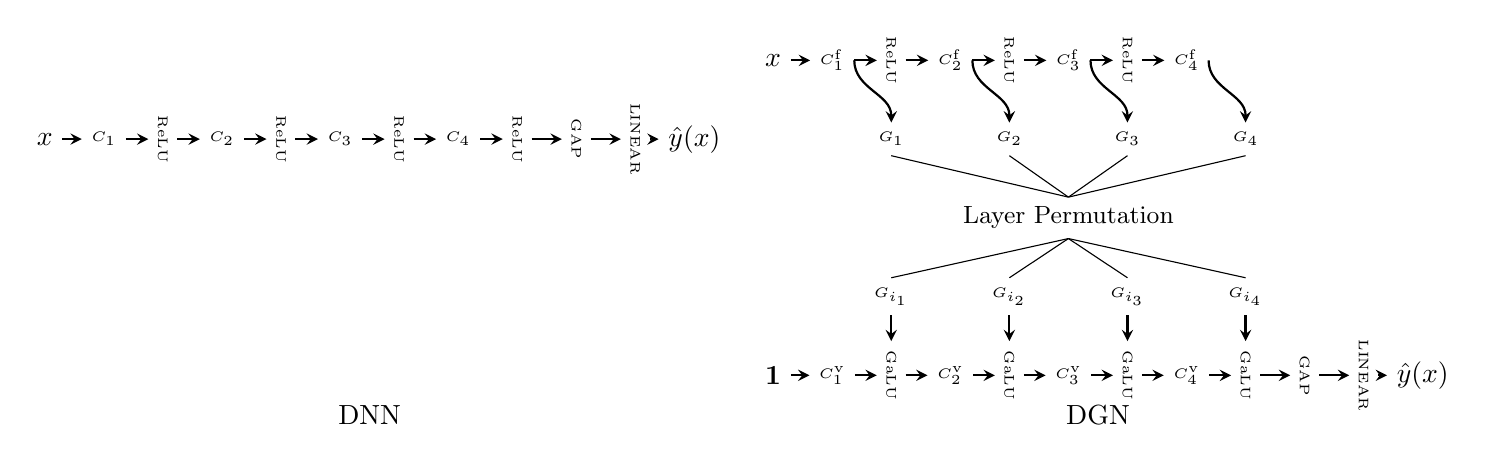
\begin{tikzpicture}
\node []  (dnn-text)at (-4.625,-3) {DNN};

\node []  (dnn-output) at (-0.5,0.5) {$\hat{y}(x)$};
\node [rotate=-90]  (dnn-smax) at (-1.25,0.5) {\tiny{LINEAR}};
\draw [-stealth,thick]   (dnn-smax.north) -- (dnn-output.west);

\node [rotate=-90]  (dnn-gap) at (-2,0.5) {\tiny{GAP}};
\draw [-stealth,thick]   (dnn-gap.north) -- (dnn-smax.south);

\node [rotate=-90] (dnn-relu-4) at (-2.75,0.5){\tiny{ReLU}};
\node [] (dnn-c4) at (-3.5,0.5){\tiny{$C_4$}};
\draw [-stealth,thick]   (dnn-c4.east) -- (dnn-relu-4.south);
\draw [-stealth,thick]   (dnn-relu-4.north) -- (dnn-gap.south);



\node [rotate=-90] (dnn-relu-3) at (-4.25,0.5){\tiny{ReLU}};
\node [] (dnn-c3) at (-5,0.5){\tiny{$C_3$}};
\draw [-stealth,thick]   (dnn-c3.east) -- (dnn-relu-3.south);
\draw [-stealth,thick]   (dnn-relu-3.north) -- (dnn-c4.west);


\node [rotate=-90] (dnn-relu-2) at (-5.75,0.5){\tiny{ReLU}};
\node [] (dnn-c2) at (-6.5,0.5){\tiny{$C_2$}};
\draw [-stealth,thick]   (dnn-c2.east) -- (dnn-relu-2.south);
\draw [-stealth,thick]   (dnn-relu-2.north) -- (dnn-c3.west);

\node [rotate=-90] (dnn-relu-1) at (-7.25,0.5){\tiny{ReLU}};
\node [] (dnn-c1) at (-8,0.5){\tiny{$C_1$}};
\draw [-stealth,thick]   (dnn-c1.east) -- (dnn-relu-1.south);
\draw [-stealth,thick]   (dnn-relu-1.north) -- (dnn-c2.west);



\node [] (dnn-input) at (-8.75,0.5){$x$};
\draw [-stealth,thick]   (dnn-input.east) -- (dnn-c1.west);


%%%%%%%%%%%%%%%%%%%%%%%%%%%%%%%%%%%%%%%%%%%%%%%%%%%%%%%%%%%%%%%%%
\node []  (fntext)at (4.625,-3) {DGN};

%\node []  (output) at (7.5,1.5) {$\hat{y}(x)$};


\node [] (dgn-f-c4) at (5.75,1.5){\tiny{$C^{\text{f}}_4$}};


\node [rotate=-90] (dgn-relu-3) at (5,1.5){\tiny{ReLU}};
\node [] (dgn-f-c3) at (4.25,1.5){\tiny{$C^{\text{f}}_3$}};
\draw [-stealth,thick]   (dgn-f-c3.east) -- (dgn-relu-3.south);
\draw [-stealth,thick]   (dgn-relu-3.north) -- (dgn-f-c4.west);


\node [rotate=-90] (dgn-relu-2) at (3.5,1.5){\tiny{ReLU}};
\node [] (dgn-f-c2) at (2.75,1.5){\tiny{$C^{\text{f}}_2$}};
\draw [-stealth,thick]   (dgn-f-c2.east) -- (dgn-relu-2.south);
\draw [-stealth,thick]   (dgn-relu-2.north) -- (dgn-f-c3.west);


\node [rotate=-90] (dgn-relu-1) at (2,1.5){\tiny{ReLU}};
\node [] (dgn-f-c1) at (1.25,1.5){\tiny{$C^{\text{f}}_1$}};
\draw [-stealth,thick]   (dgn-f-c1.east) -- (dgn-relu-1.south);
\draw [-stealth,thick]   (dgn-relu-1.north) -- (dgn-f-c2.west);



\node [] (dgn-f-input) at (0.5,1.5){$x$};
\draw [-stealth,thick]   (dgn-f-input.east) -- (dgn-f-c1.west);




\node []  (dgn-output) at (8.75,-2.5) {$\hat{y}(x)$};
\node [rotate=-90] (dgn-smax) at (8,-2.5){\tiny{LINEAR}};
\draw [-stealth,thick]   (dgn-smax.north)--(dgn-output.west);

\node [rotate=-90] (dgn-gap) at (7.25,-2.5){\tiny{GAP}};
\draw [-stealth,thick]   (dgn-gap.north)--(dgn-smax.south);



\node [rotate=-90] (dgn-galu-4) at (6.5,-2.5){\tiny{GaLU}};
\draw [-stealth,thick]   (dgn-galu-4.north) -- (dgn-gap.south);

\node [] (dgn-v-c4) at (5.75,-2.5){\tiny{$C^{\text{v}}_4$}};
\draw [-stealth,thick]   (dgn-v-c4.east) -- (dgn-galu-4.south);

\node [rotate=-90] (dgn-galu-3) at (5,-2.5){\tiny{GaLU}};
\node [] (dgn-v-c3) at (4.25,-2.5){\tiny{$C^{\text{v}}_3$}};
\draw [-stealth,thick]   (dgn-v-c3.east) -- (dgn-galu-3.south);
\draw [-stealth,thick]   (dgn-galu-3.north) -- (dgn-v-c4.west);



\node [rotate=-90] (dgn-galu-2) at (3.5,-2.5){\tiny{GaLU}};
\node [] (dgn-v-c2) at (2.75,-2.5){\tiny{$C^{\text{v}}_2$}};
\draw [-stealth,thick]   (dgn-v-c2.east) -- (dgn-galu-2.south);
\draw [-stealth,thick]   (dgn-galu-2.north) -- (dgn-v-c3.west);


\node [rotate=-90] (dgn-galu-1) at (2,-2.5){\tiny{GaLU}};
\node [] (dgn-v-c1) at (1.25,-2.5){\tiny{$C^{\text{v}}_1$}};

\draw [-stealth,thick]   (dgn-v-c1.east) -- (dgn-galu-1.south);
\draw [-stealth,thick]   (dgn-galu-1.north) -- (dgn-v-c2.west);




\node [] (dgn-input) at (0.5,-2.5){$\mathbf{1}$};
\draw [-stealth,thick]   (dgn-input.east) -- (dgn-v-c1.west);


\node[] (dgn-gating-1-up) at (2,0.5){\tiny{$G_{1}$}};
\draw [-stealth,thick]   (dgn-f-c1.east) to[out=-90,in=90] (dgn-gating-1-up.north);


\node[] (dgn-gating-2-up) at (3.5,0.5){\tiny{$G_{2}$}};
\draw [-stealth,thick]   (dgn-f-c2.east) to[out=-90,in=90] (dgn-gating-2-up.north);



\node[] (dgn-gating-3-up) at (5,0.5){\tiny{$G_{3}$}};
\draw [-stealth,thick]   (dgn-f-c3.east) to[out=-90,in=90] (dgn-gating-3-up.north);


\node[] (dgn-gating-4-up) at (6.5,0.5){\tiny{$G_{4}$}};
\draw [-stealth,thick]   (dgn-f-c4.east) to[out=-90,in=90] (dgn-gating-4-up.north);





\node[] (dgn-gating-1) at (2,-1.5){\tiny{$G_{i_1}$}};
\draw [-stealth,thick]   (dgn-gating-1.south) -- (dgn-galu-1.west);


\node[] (dgn-gating-2) at (3.5,-1.5){\tiny{$G_{i_2}$}};
\draw [-stealth,thick]   (dgn-gating-2.south) -- (dgn-galu-2.west);



\node[] (dgn-gating-3) at (5,-1.5){\tiny{$G_{i_3}$}};
\draw [-stealth,thick]   (dgn-gating-3.south) -- (dgn-galu-3.west);


\node[] (dgn-gating-4) at (6.5,-1.5){\tiny{$G_{i_4}$}};
\draw [-stealth,thick]   (dgn-gating-4.south) -- (dgn-galu-4.west);



\node[] (permutation) at (4.25,-0.5){\small{Layer Permutation}};

\draw [-]   (dgn-gating-1-up.south) -- (permutation.north);
\draw [-]   (dgn-gating-4-up.south) -- (permutation.north);
\draw [-]   (dgn-gating-2-up.south) -- (permutation.north);
\draw [-]   (dgn-gating-3-up.south) -- (permutation.north);



\draw [-]  (permutation.south) --  (dgn-gating-1.north)  ;
\draw [-]  (permutation.south) --  (dgn-gating-2.north)  ;
\draw [-]  (permutation.south) --  (dgn-gating-3.north)  ;
\draw [-]  (permutation.south) --  (dgn-gating-4.north)  ;

	
\end{tikzpicture}


}
\resizebox{0.99\columnwidth}{!}{
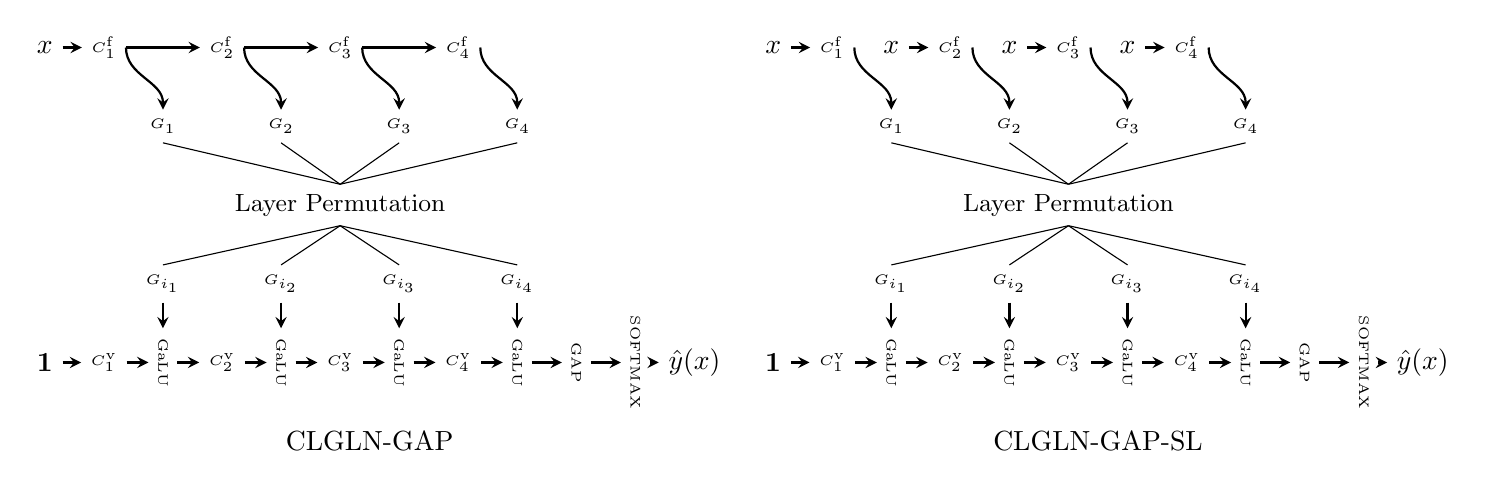
\begin{tikzpicture}
\node []  (fntext)at (-4.625,-3.5) {CLGLN-GAP};

%\node []  (output) at (7.5,1.5) {$\hat{y}(x)$};


\node [] (dgn1-f-c4) at (-3.5,1.5){\tiny{$C^{\text{f}}_4$}};
\node [] (dgn1-f-c3) at (-5,1.5){\tiny{$C^{\text{f}}_3$}};
\node [] (dgn1-f-c2) at (-6.5,1.5){\tiny{$C^{\text{f}}_2$}};
\node [] (dgn1-f-c1) at (-8,1.5){\tiny{$C^{\text{f}}_1$}};
\node [] (dgn1-input-f) at (-8.75,1.5){$x$};
\draw [-stealth,thick]   (dgn1-f-c3.east) -- (dgn1-f-c4.west);
\draw [-stealth,thick]   (dgn1-f-c2.east) -- (dgn1-f-c3.west);
\draw [-stealth,thick]   (dgn1-f-c1.east) -- (dgn1-f-c2.west);
\draw [-stealth,thick]   (dgn1-input-f.east) -- (dgn1-f-c1.west);



\node []  (dgn1-output) at (-0.5,-2.5) {$\hat{y}(x)$};

\node [rotate=-90] (dgn1-smax) at (-1.25,-2.5){\tiny{SOFTMAX}};
\draw [-stealth,thick]   (dgn1-smax.north)--(dgn1-output.west);

\node [rotate=-90] (dgn1-gap) at (-2,-2.5){\tiny{GAP}};
\draw [-stealth,thick]   (dgn1-gap.north)--(dgn1-smax.south);


\node [rotate=-90] (dgn1-galu-4) at (-2.75,-2.5){\tiny{GaLU}};
\draw [-stealth,thick]   (dgn1-galu-4.north)--(dgn1-gap.south);

\node [] (dgn1-v-c4) at (-3.5,-2.5){\tiny{$C^{\text{v}}_4$}};
\draw [-stealth,thick]   (dgn1-v-c4.east) -- (dgn1-galu-4.south);


\node [rotate=-90] (dgn1-galu-3) at (-4.25,-2.5){\tiny{GaLU}};
\draw [-stealth,thick]   (dgn1-galu-3.north) -- (dgn1-v-c4.west);

\node [] (dgn1-v-c3) at (-5,-2.5){\tiny{$C^{\text{v}}_3$}};
\draw [-stealth,thick]   (dgn1-v-c3.east) -- (dgn1-galu-3.south);


\node [rotate=-90] (dgn1-galu-2) at (-5.75,-2.5){\tiny{GaLU}};
\draw [-stealth,thick]   (dgn1-galu-2.north) -- (dgn1-v-c3.west);

\node [] (dgn1-v-c2) at (-6.5,-2.5){\tiny{$C^{\text{v}}_2$}};
\draw [-stealth,thick]   (dgn1-v-c2.east) -- (dgn1-galu-2.south);


\node [rotate=-90] (dgn1-galu-1) at (-7.25,-2.5){\tiny{GaLU}};
\draw [-stealth,thick]   (dgn1-galu-1.north) -- (dgn1-v-c2.west);


\node [] (dgn1-v-c1) at (-8,-2.5){\tiny{$C^{\text{v}}_1$}};
\draw [-stealth,thick]   (dgn1-v-c1.east) -- (dgn1-galu-1.south);


\node [] (dgn1-v-input) at (-8.75,-2.5){$\mathbf{1}$};

\draw [-stealth,thick]   (dgn1-v-input.east) -- (dgn1-v-c1.west);


\node[] (dgn1-gating-4-up) at (-2.75,0.5){\tiny{$G_{4}$}};
\draw [-stealth,thick]   (dgn1-f-c4.east) to[out=-90,in=90] (dgn1-gating-4-up.north);


\node[] (dgn1-gating-3-up) at (-4.25,0.5){\tiny{$G_{3}$}};
\draw [-stealth,thick]   (dgn1-f-c3.east) to[out=-90,in=90] (dgn1-gating-3-up.north);



\node[] (dgn1-gating-2-up) at (-5.75,0.5){\tiny{$G_{2}$}};
\draw [-stealth,thick]   (dgn1-f-c2.east) to[out=-90,in=90] (dgn1-gating-2-up.north);


\node[] (dgn1-gating-1-up) at (-7.25,0.5){\tiny{$G_{1}$}};
\draw [-stealth,thick]   (dgn1-f-c1.east) to[out=-90,in=90] (dgn1-gating-1-up.north);





\node[] (dgn1-gating-4) at (-2.75,-1.5){\tiny{$G_{i_4}$}};
\draw [-stealth,thick]   (dgn1-gating-4.south) -- (dgn1-galu-4.west);


\node[] (dgn1-gating-3) at (-4.25,-1.5){\tiny{$G_{i_3}$}};
\draw [-stealth,thick]   (dgn1-gating-3.south) -- (dgn1-galu-3.west);



\node[] (dgn1-gating-2) at (-5.75,-1.5){\tiny{$G_{i_2}$}};
\draw [-stealth,thick]   (dgn1-gating-2.south) -- (dgn1-galu-2.west);


\node[] (dgn1-gating-1) at (-7.25,-1.5){\tiny{$G_{i_1}$}};
\draw [-stealth,thick]   (dgn1-gating-1.south) -- (dgn1-galu-1.west);



\node[] (permutation1) at (-5,-0.5){\small{Layer Permutation}};

\draw [-]   (dgn1-gating-1-up.south) -- (permutation1.north);
\draw [-]   (dgn1-gating-4-up.south) -- (permutation1.north);
\draw [-]   (dgn1-gating-2-up.south) -- (permutation1.north);
\draw [-]   (dgn1-gating-3-up.south) -- (permutation1.north);



\draw [-]  (permutation1.south) --  (dgn1-gating-1.north)  ;
\draw [-]  (permutation1.south) --  (dgn1-gating-2.north)  ;
\draw [-]  (permutation1.south) --  (dgn1-gating-3.north)  ;
\draw [-]  (permutation1.south) --  (dgn1-gating-4.north)  ;


%%%%%%%%%%%%%%%%%%%%%%%%%%%%%%%%%%%%%%%%%%%%%%%%%%%%%%%%%%%%%%%%%
\node []  (fntext)at (4.625,-3.5) {CLGLN-GAP-SL};

%\node []  (output) at (7.5,1.5) {$\hat{y}(x)$};

\node [] (dgn-f-input) at (0.5,1.5){$x$};
\node [] (dgn-f-c4) at (5.75,1.5){\tiny{$C^{\text{f}}_4$}};

\node [] (dgn-f-x-4) at (5,1.5){$x$};


\node [] (dgn-f-c3) at (4.25,1.5){\tiny{$C^{\text{f}}_3$}};
\node [] (dgn-f-x-3) at (3.5,1.5){$x$};

\node [] (dgn-f-c2) at (2.75,1.5){\tiny{$C^{\text{f}}_2$}};
\node [] (dgn-f-x-2) at (2,1.5){$x$};

\node [] (dgn-f-c1) at (1.25,1.5){\tiny{$C^{\text{f}}_1$}};

\draw [-stealth,thick]   (dgn-f-input.east) -- (dgn-f-c1.west);
\draw [-stealth,thick]   (dgn-f-x-2.east) -- (dgn-f-c2.west);
\draw [-stealth,thick]   (dgn-f-x-3.east) -- (dgn-f-c3.west);
\draw [-stealth,thick]   (dgn-f-x-4.east) -- (dgn-f-c4.west);


\node []  (dgn-output) at (8.75,-2.5) {$\hat{y}(x)$};



\node [rotate=-90] (dgn-smax) at (8,-2.5){\tiny{SOFTMAX}};
\draw [-stealth,thick]   (dgn-smax.north) -- (dgn-output.west);
;
\node [rotate=-90] (dgn-gap) at (7.25,-2.5){\tiny{GAP}};
\draw [-stealth,thick]   (dgn-gap.north) -- (dgn-smax.south);



\node [rotate=-90] (dgn-galu-4) at (6.5,-2.5){\tiny{GaLU}};

\draw [-stealth,thick]   (dgn-galu-4.north) -- (dgn-gap.south);
\node [] (dgn-v-c4) at (5.75,-2.5){\tiny{$C^{\text{v}}_4$}};
\draw [-stealth,thick]   (dgn-v-c4.east) -- (dgn-galu-4.south);


\node [rotate=-90] (dgn-galu-3) at (5,-2.5){\tiny{GaLU}};
\draw [-stealth,thick]   (dgn-galu-3.north) -- (dgn-v-c4.west);


\node [] (dgn-v-c3) at (4.25,-2.5){\tiny{$C^{\text{v}}_3$}};
\draw [-stealth,thick]   (dgn-v-c3.east) -- (dgn-galu-3.south);


\node [rotate=-90] (dgn-galu-2) at (3.5,-2.5){\tiny{GaLU}};
\draw [-stealth,thick]   (dgn-galu-2.north) -- (dgn-v-c3.west);

\node [] (dgn-v-c2) at (2.75,-2.5){\tiny{$C^{\text{v}}_2$}};
\draw [-stealth,thick]   (dgn-v-c2.east) -- (dgn-galu-2.south);


\node [rotate=-90] (dgn-galu-1) at (2.0,-2.5){\tiny{GaLU}};
\draw [-stealth,thick]   (dgn-galu-1.north) -- (dgn-v-c2.west);

\node [] (dgn-v-c1) at (1.25,-2.5){\tiny{$C^{\text{v}}_1$}};
\draw [-stealth,thick]   (dgn-v-c1.east) -- (dgn-galu-1.south);


\node [] (dgn-v-input) at (0.5,-2.5){$\mathbf{1}$};

\draw [-stealth,thick]   (dgn-v-input.east) -- (dgn-v-c1.west);


\node[] (dgn-gating-1-up) at (2,0.5){\tiny{$G_{1}$}};
\draw [-stealth,thick]   (dgn-f-c1.east) to[out=-90,in=90] (dgn-gating-1-up.north);


\node[] (dgn-gating-2-up) at (3.5,0.5){\tiny{$G_{2}$}};
\draw [-stealth,thick]   (dgn-f-c2.east) to[out=-90,in=90] (dgn-gating-2-up.north);



\node[] (dgn-gating-3-up) at (5,0.5){\tiny{$G_{3}$}};
\draw [-stealth,thick]   (dgn-f-c3.east) to[out=-90,in=90] (dgn-gating-3-up.north);


\node[] (dgn-gating-4-up) at (6.5,0.5){\tiny{$G_{4}$}};
\draw [-stealth,thick]   (dgn-f-c4.east) to[out=-90,in=90] (dgn-gating-4-up.north);





\node[] (dgn-gating-1) at (2,-1.5){\tiny{$G_{i_1}$}};
\draw [-stealth,thick]   (dgn-gating-1.south) -- (dgn-galu-1.west);


\node[] (dgn-gating-2) at (3.5,-1.5){\tiny{$G_{i_2}$}};
\draw [-stealth,thick]   (dgn-gating-2.south) -- (dgn-galu-2.west);



\node[] (dgn-gating-3) at (5,-1.5){\tiny{$G_{i_3}$}};
\draw [-stealth,thick]   (dgn-gating-3.south) -- (dgn-galu-3.west);


\node[] (dgn-gating-4) at (6.5,-1.5){\tiny{$G_{i_4}$}};
\draw [-stealth,thick]   (dgn-gating-4.south) -- (dgn-galu-4.west);



\node[] (permutation) at (4.25,-0.5){\small{Layer Permutation}};

\draw [-]   (dgn-gating-1-up.south) -- (permutation.north);
\draw [-]   (dgn-gating-4-up.south) -- (permutation.north);
\draw [-]   (dgn-gating-2-up.south) -- (permutation.north);
\draw [-]   (dgn-gating-3-up.south) -- (permutation.north);



\draw [-]  (permutation.south) --  (dgn-gating-1.north)  ;
\draw [-]  (permutation.south) --  (dgn-gating-2.north)  ;
\draw [-]  (permutation.south) --  (dgn-gating-3.north)  ;
\draw [-]  (permutation.south) --  (dgn-gating-4.north)  ;



	
\end{tikzpicture}


}
\end{minipage}
\caption{$4$ convolutional layers with GAP}
\label{fig:c4gap}
\end{figure}




\begin{figure}[!t]
\centering
\begin{minipage}{1.0\columnwidth}
\centering
\begin{minipage}{0.49\columnwidth}
\resizebox{0.99\columnwidth}{!}{
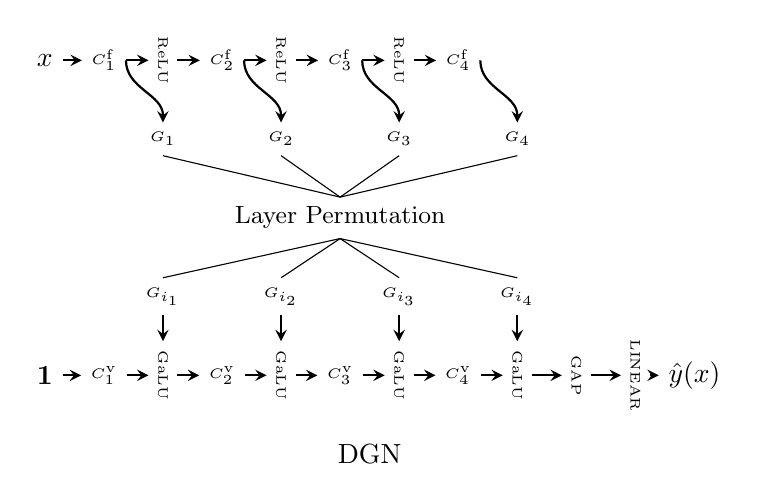
\begin{tikzpicture}
%%%%%%%%%%%%%%%%%%%%%%%%%%%%%%%%%%%%%%%%%%%%%%%%%%%%%%%%%%%%%%%%%
\node []  (fntext)at (4.625,-3.5) {DGN};

%\node []  (output) at (7.5,1.5) {$\hat{y}(x)$};


\node [] (dgn-f-c4) at (5.75,1.5){\tiny{$C^{\text{f}}_4$}};


\node [rotate=-90] (dgn-relu-3) at (5,1.5){\tiny{ReLU}};
\node [] (dgn-f-c3) at (4.25,1.5){\tiny{$C^{\text{f}}_3$}};
\draw [-stealth,thick]   (dgn-f-c3.east) -- (dgn-relu-3.south);
\draw [-stealth,thick]   (dgn-relu-3.north) -- (dgn-f-c4.west);


\node [rotate=-90] (dgn-relu-2) at (3.5,1.5){\tiny{ReLU}};
\node [] (dgn-f-c2) at (2.75,1.5){\tiny{$C^{\text{f}}_2$}};
\draw [-stealth,thick]   (dgn-f-c2.east) -- (dgn-relu-2.south);
\draw [-stealth,thick]   (dgn-relu-2.north) -- (dgn-f-c3.west);


\node [rotate=-90] (dgn-relu-1) at (2,1.5){\tiny{ReLU}};
\node [] (dgn-f-c1) at (1.25,1.5){\tiny{$C^{\text{f}}_1$}};
\draw [-stealth,thick]   (dgn-f-c1.east) -- (dgn-relu-1.south);
\draw [-stealth,thick]   (dgn-relu-1.north) -- (dgn-f-c2.west);



\node [] (dgn-f-input) at (0.5,1.5){$x$};
\draw [-stealth,thick]   (dgn-f-input.east) -- (dgn-f-c1.west);




\node []  (dgn-output) at (8.75,-2.5) {$\hat{y}(x)$};
\node [rotate=-90] (dgn-smax) at (8,-2.5){\tiny{LINEAR}};
\draw [-stealth,thick]   (dgn-smax.north)--(dgn-output.west);

\node [rotate=-90] (dgn-gap) at (7.25,-2.5){\tiny{GAP}};
\draw [-stealth,thick]   (dgn-gap.north)--(dgn-smax.south);



\node [rotate=-90] (dgn-galu-4) at (6.5,-2.5){\tiny{GaLU}};
\draw [-stealth,thick]   (dgn-galu-4.north) -- (dgn-gap.south);

\node [] (dgn-v-c4) at (5.75,-2.5){\tiny{$C^{\text{v}}_4$}};
\draw [-stealth,thick]   (dgn-v-c4.east) -- (dgn-galu-4.south);

\node [rotate=-90] (dgn-galu-3) at (5,-2.5){\tiny{GaLU}};
\node [] (dgn-v-c3) at (4.25,-2.5){\tiny{$C^{\text{v}}_3$}};
\draw [-stealth,thick]   (dgn-v-c3.east) -- (dgn-galu-3.south);
\draw [-stealth,thick]   (dgn-galu-3.north) -- (dgn-v-c4.west);



\node [rotate=-90] (dgn-galu-2) at (3.5,-2.5){\tiny{GaLU}};
\node [] (dgn-v-c2) at (2.75,-2.5){\tiny{$C^{\text{v}}_2$}};
\draw [-stealth,thick]   (dgn-v-c2.east) -- (dgn-galu-2.south);
\draw [-stealth,thick]   (dgn-galu-2.north) -- (dgn-v-c3.west);


\node [rotate=-90] (dgn-galu-1) at (2,-2.5){\tiny{GaLU}};
\node [] (dgn-v-c1) at (1.25,-2.5){\tiny{$C^{\text{v}}_1$}};

\draw [-stealth,thick]   (dgn-v-c1.east) -- (dgn-galu-1.south);
\draw [-stealth,thick]   (dgn-galu-1.north) -- (dgn-v-c2.west);




\node [] (dgn-input) at (0.5,-2.5){$\mathbf{1}$};
\draw [-stealth,thick]   (dgn-input.east) -- (dgn-v-c1.west);


\node[] (dgn-gating-1-up) at (2,0.5){\tiny{$G_{1}$}};
\draw [-stealth,thick]   (dgn-f-c1.east) to[out=-90,in=90] (dgn-gating-1-up.north);


\node[] (dgn-gating-2-up) at (3.5,0.5){\tiny{$G_{2}$}};
\draw [-stealth,thick]   (dgn-f-c2.east) to[out=-90,in=90] (dgn-gating-2-up.north);



\node[] (dgn-gating-3-up) at (5,0.5){\tiny{$G_{3}$}};
\draw [-stealth,thick]   (dgn-f-c3.east) to[out=-90,in=90] (dgn-gating-3-up.north);


\node[] (dgn-gating-4-up) at (6.5,0.5){\tiny{$G_{4}$}};
\draw [-stealth,thick]   (dgn-f-c4.east) to[out=-90,in=90] (dgn-gating-4-up.north);





\node[] (dgn-gating-1) at (2,-1.5){\tiny{$G_{i_1}$}};
\draw [-stealth,thick]   (dgn-gating-1.south) -- (dgn-galu-1.west);


\node[] (dgn-gating-2) at (3.5,-1.5){\tiny{$G_{i_2}$}};
\draw [-stealth,thick]   (dgn-gating-2.south) -- (dgn-galu-2.west);



\node[] (dgn-gating-3) at (5,-1.5){\tiny{$G_{i_3}$}};
\draw [-stealth,thick]   (dgn-gating-3.south) -- (dgn-galu-3.west);


\node[] (dgn-gating-4) at (6.5,-1.5){\tiny{$G_{i_4}$}};
\draw [-stealth,thick]   (dgn-gating-4.south) -- (dgn-galu-4.west);



\node[] (permutation) at (4.25,-0.5){\small{Layer Permutation}};

\draw [-]   (dgn-gating-1-up.south) -- (permutation.north);
\draw [-]   (dgn-gating-4-up.south) -- (permutation.north);
\draw [-]   (dgn-gating-2-up.south) -- (permutation.north);
\draw [-]   (dgn-gating-3-up.south) -- (permutation.north);



\draw [-]  (permutation.south) --  (dgn-gating-1.north)  ;
\draw [-]  (permutation.south) --  (dgn-gating-2.north)  ;
\draw [-]  (permutation.south) --  (dgn-gating-3.north)  ;
\draw [-]  (permutation.south) --  (dgn-gating-4.north)  ;

	
\end{tikzpicture}


}
\end{minipage}
\begin{minipage}{0.49\columnwidth}
\resizebox{0.99\columnwidth}{!}{
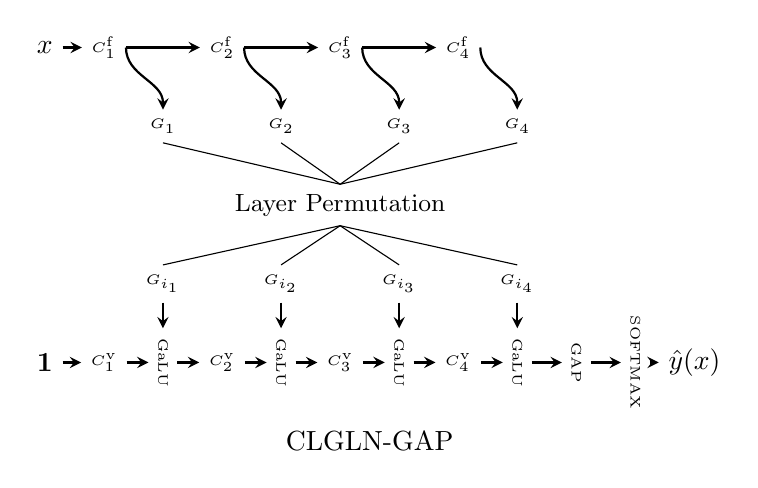
\begin{tikzpicture}
\node []  (fntext)at (-4.625,-3.5) {CLGLN-GAP};

%\node []  (output) at (7.5,1.5) {$\hat{y}(x)$};


\node [] (dgn1-f-c4) at (-3.5,1.5){\tiny{$C^{\text{f}}_4$}};
\node [] (dgn1-f-c3) at (-5,1.5){\tiny{$C^{\text{f}}_3$}};
\node [] (dgn1-f-c2) at (-6.5,1.5){\tiny{$C^{\text{f}}_2$}};
\node [] (dgn1-f-c1) at (-8,1.5){\tiny{$C^{\text{f}}_1$}};
\node [] (dgn1-input-f) at (-8.75,1.5){$x$};
\draw [-stealth,thick]   (dgn1-f-c3.east) -- (dgn1-f-c4.west);
\draw [-stealth,thick]   (dgn1-f-c2.east) -- (dgn1-f-c3.west);
\draw [-stealth,thick]   (dgn1-f-c1.east) -- (dgn1-f-c2.west);
\draw [-stealth,thick]   (dgn1-input-f.east) -- (dgn1-f-c1.west);



\node []  (dgn1-output) at (-0.5,-2.5) {$\hat{y}(x)$};

\node [rotate=-90] (dgn1-smax) at (-1.25,-2.5){\tiny{SOFTMAX}};
\draw [-stealth,thick]   (dgn1-smax.north)--(dgn1-output.west);

\node [rotate=-90] (dgn1-gap) at (-2,-2.5){\tiny{GAP}};
\draw [-stealth,thick]   (dgn1-gap.north)--(dgn1-smax.south);


\node [rotate=-90] (dgn1-galu-4) at (-2.75,-2.5){\tiny{GaLU}};
\draw [-stealth,thick]   (dgn1-galu-4.north)--(dgn1-gap.south);

\node [] (dgn1-v-c4) at (-3.5,-2.5){\tiny{$C^{\text{v}}_4$}};
\draw [-stealth,thick]   (dgn1-v-c4.east) -- (dgn1-galu-4.south);


\node [rotate=-90] (dgn1-galu-3) at (-4.25,-2.5){\tiny{GaLU}};
\draw [-stealth,thick]   (dgn1-galu-3.north) -- (dgn1-v-c4.west);

\node [] (dgn1-v-c3) at (-5,-2.5){\tiny{$C^{\text{v}}_3$}};
\draw [-stealth,thick]   (dgn1-v-c3.east) -- (dgn1-galu-3.south);


\node [rotate=-90] (dgn1-galu-2) at (-5.75,-2.5){\tiny{GaLU}};
\draw [-stealth,thick]   (dgn1-galu-2.north) -- (dgn1-v-c3.west);

\node [] (dgn1-v-c2) at (-6.5,-2.5){\tiny{$C^{\text{v}}_2$}};
\draw [-stealth,thick]   (dgn1-v-c2.east) -- (dgn1-galu-2.south);


\node [rotate=-90] (dgn1-galu-1) at (-7.25,-2.5){\tiny{GaLU}};
\draw [-stealth,thick]   (dgn1-galu-1.north) -- (dgn1-v-c2.west);


\node [] (dgn1-v-c1) at (-8,-2.5){\tiny{$C^{\text{v}}_1$}};
\draw [-stealth,thick]   (dgn1-v-c1.east) -- (dgn1-galu-1.south);


\node [] (dgn1-v-input) at (-8.75,-2.5){$\mathbf{1}$};

\draw [-stealth,thick]   (dgn1-v-input.east) -- (dgn1-v-c1.west);


\node[] (dgn1-gating-4-up) at (-2.75,0.5){\tiny{$G_{4}$}};
\draw [-stealth,thick]   (dgn1-f-c4.east) to[out=-90,in=90] (dgn1-gating-4-up.north);


\node[] (dgn1-gating-3-up) at (-4.25,0.5){\tiny{$G_{3}$}};
\draw [-stealth,thick]   (dgn1-f-c3.east) to[out=-90,in=90] (dgn1-gating-3-up.north);



\node[] (dgn1-gating-2-up) at (-5.75,0.5){\tiny{$G_{2}$}};
\draw [-stealth,thick]   (dgn1-f-c2.east) to[out=-90,in=90] (dgn1-gating-2-up.north);


\node[] (dgn1-gating-1-up) at (-7.25,0.5){\tiny{$G_{1}$}};
\draw [-stealth,thick]   (dgn1-f-c1.east) to[out=-90,in=90] (dgn1-gating-1-up.north);





\node[] (dgn1-gating-4) at (-2.75,-1.5){\tiny{$G_{i_4}$}};
\draw [-stealth,thick]   (dgn1-gating-4.south) -- (dgn1-galu-4.west);


\node[] (dgn1-gating-3) at (-4.25,-1.5){\tiny{$G_{i_3}$}};
\draw [-stealth,thick]   (dgn1-gating-3.south) -- (dgn1-galu-3.west);



\node[] (dgn1-gating-2) at (-5.75,-1.5){\tiny{$G_{i_2}$}};
\draw [-stealth,thick]   (dgn1-gating-2.south) -- (dgn1-galu-2.west);


\node[] (dgn1-gating-1) at (-7.25,-1.5){\tiny{$G_{i_1}$}};
\draw [-stealth,thick]   (dgn1-gating-1.south) -- (dgn1-galu-1.west);



\node[] (permutation1) at (-5,-0.5){\small{Layer Permutation}};

\draw [-]   (dgn1-gating-1-up.south) -- (permutation1.north);
\draw [-]   (dgn1-gating-4-up.south) -- (permutation1.north);
\draw [-]   (dgn1-gating-2-up.south) -- (permutation1.north);
\draw [-]   (dgn1-gating-3-up.south) -- (permutation1.north);



\draw [-]  (permutation1.south) --  (dgn1-gating-1.north)  ;
\draw [-]  (permutation1.south) --  (dgn1-gating-2.north)  ;
\draw [-]  (permutation1.south) --  (dgn1-gating-3.north)  ;
\draw [-]  (permutation1.south) --  (dgn1-gating-4.north)  ;


%%%%%%%%%%%%%%%%%%%%%%%%%%%%%%%%%%%%%%%%%%%%%%%%%%%%%%%%%%%%%%%%%

	
\end{tikzpicture}


}
\end{minipage}
\end{minipage}
\caption{$4$ convolutional layers with GAP}
\label{fig:c4gap}
\end{figure}
\end{comment}

\begin{table}[!t]
\centering
\resizebox{1.0\columnwidth}{!}{
\begin{tabular}{cccccccc}
\toprule 
Dataset 					& C4GAP 		&DNN 				&DGN$(x,x)$ 			&DGN$(x,\mathbf{1})$ 	&DLGN$(x,x)$ 			&DLGN$(x,\mathbf{1})$ 	&Recovery\\\midrule
\multirow{2}{*}{CIFAR10}		& Vanilla		&80.5\tiny{$\pm$0.4} 	&77.4\tiny{$\pm$0.3} 	& 77.5\tiny{$\pm$0.2} 	&75.4\tiny{$\pm$0.3} 	&75.4\tiny{$\pm$0.2}		&$93.66\%$	\\
						& Permute 	&-- 					&77.3\tiny{$\pm$0.5} 	&77.9\tiny{$\pm$0.6}		&75.9\tiny{$\pm$0.5} 	&76.0\tiny{$\pm$0.5}		&$94.40\%$	\\					%\midrule
%\multirow{2}{*}{CIFAR100}		& Vanilla  				&51.8\tiny{$\pm$0.4} 	&47.4\tiny{$\pm$0.2}		&47.3\tiny{$\pm$0.3} 	&47.4\tiny{$\pm$0.1} 	&48.0\tiny{$\pm$0.2}		\\
%						& Permute 	& -- 		&48.4\tiny{$\pm$0.8} 	&49.2\tiny{$\pm$0.9} 	&47.5\tiny{$\pm$1.0} 	&48.4\tiny{$\pm$0.9}		\\
\bottomrule
\end{tabular}
}
\caption{\small{Top row shows results for vanilla models without permutations; the results are averaged over $5$ runs. The bottom row shows results of $4!-1=24-1=23$ permutations (other than the identity permutation) for each model; the results are averaged over the $23$ permutations.}}
\label{tb:permute}
\end{table}

\begin{table}[!t]
\centering
\resizebox{1.0\columnwidth}{!}{
\begin{tabular}{cccccccccc}
\toprule 
Dataset 					& Model 		&DNN 				&DGN$(x,x)$ 			&DGN$(x,\mathbf{1})$ 	&DLGN$(x,x)$ 			&DLGN$(x,\mathbf{1})$ 	&Recovery\\\midrule		
\multirow{2}{*}{CIFAR10}		&VGG16 		&93.6\tiny{$\pm$0.2} 	& 93.0\tiny{$\pm$0.1}  	&93.0\tiny{$\pm$0.1}   	&87.0\tiny{$\pm$0.1}		&87.0\tiny{$\pm$0.2}		&$92.94\%$	\\
						&ResNet110 	&94.0\tiny{$\pm$0.2} 	& 93.3\tiny{$\pm$0.2} 	&93.2\tiny{$\pm$0.1} 	&87.9\tiny{$\pm$0.2}   	&87.8\tiny{$\pm$0.1} 	&$93.40\%$	\\\midrule
\multirow{2}{*}{CIFAR100}		&VGG16	 	&73.4\tiny{$\pm$0.3}  	&70.3\tiny{$\pm$0.1} 	&70.5\tiny{$\pm$0.2} 	&61.5\tiny{$\pm$0.2}		&61.5\tiny{$\pm$0.1}		&$\mathbf{83.78\%}$	\\
						&ResNet110 	&72.7\tiny{$\pm$0.2}		&70.8\tiny{$\pm$0.2} 	&70.8\tiny{$\pm$0.4}		&62.3\tiny{$\pm$0.2} 	&62.7\tiny{$\pm$0.3} 	&$86.24\%$	\\
\bottomrule
\end{tabular}
}
\caption{Summary of Experiments}
\label{tb:expresults}
\end{table}


\begin{comment}
\begin{table}[!t]
\centering
\resizebox{1.0\columnwidth}{!}{
\begin{tabular}{ccccccccc}
\toprule 
Dataset 					& Model 				&DNN 				&DGN$(x,x)$ 			&DGN$(x,\mathbf{1})$ 	&DLGN$(x,x)$ 			&DLGN$(x,\mathbf{1})$ 	&DSLGN$(x,x)$ 		&DSLGN$(x,\mathbf{1})$  \\\midrule
\multirow{2}{*}{CIFAR10}		& C4GAP 				&80.5\tiny{$\pm$0.4} 	&77.4\tiny{$\pm$0.3} 	& 77.5\tiny{$\pm$0.2} 	&75.4\tiny{$\pm$0.3} 	&75.4\tiny{$\pm$0.2}		&74.2\tiny{$\pm$0.2}	 	&73.3\tiny{$\pm$0.2} \\
						& C4GAP-PERMUTE 	&-- 					&77.3\tiny{$\pm$0.5} 	&77.9\tiny{$\pm$0.6}		&75.9\tiny{$\pm$0.5} 	&76.0\tiny{$\pm$0.5}		& -- 					& -- \\\midrule
\multirow{2}{*}{CIFAR100}		& C4GAP 				&51.8\tiny{$\pm$0.4} 	&47.4\tiny{$\pm$0.2}		&47.3\tiny{$\pm$0.3} 	&47.4\tiny{$\pm$0.1} 	&48.0\tiny{$\pm$0.2}		&45.8\tiny{$\pm$0.3}	 	&44.9\tiny{$\pm$0.1}	\\
						& C4GAP-PERMUTE 	& -- 					&48.4\tiny{$\pm$0.8} 	&49.2\tiny{$\pm$0.9} 	&47.5\tiny{$\pm$1.0} 	&48.4\tiny{$\pm$0.9}		& --					& -- \\
\bottomrule
\end{tabular}
}
\caption{Summary of Experiments}
\label{tb:premresults}
\end{table}

\begin{table}[!t]
\centering
\resizebox{1.0\columnwidth}{!}{
\begin{tabular}{ccccccccc}
\toprule 
Dataset 					& Model 		&DNN 				&DGN$(x,x)$ 			&DGN$(x,\mathbf{1})$ 	&DLGN$(x,x)$ 			&DLGN$(x,\mathbf{1})$ 	&DSLGN$(x,x)$ 		&DSLGN$(x,\mathbf{1})$  \\\midrule		
\multirow{2}{*}{CIFAR10}		&VGG16-AP 	&93.6\tiny{$\pm$0.2} 	& 93.0\tiny{$\pm$0.1}  	&93.0\tiny{$\pm$0.1}   	&87.0\tiny{$\pm$0.1}		&87.0\tiny{$\pm$0.2}		&84.8\tiny{$\pm$0.3} 	&84.9\tiny{$\pm$0.2} \\
						&ResNet110 	&94.0\tiny{$\pm$0.2} 	& 93.3\tiny{$\pm$0.2} 	&93.2\tiny{$\pm$0.1} 	&87.9\tiny{$\pm$0.2}   	&87.8\tiny{$\pm$0.1} 	&72.4{$\pm$13.8} 		&71.2{$\pm$17.3}  \\\midrule
\multirow{2}{*}{CIFAR100}		&VGG16-AP 	&73.4\tiny{$\pm$0.3}  	&70.3\tiny{$\pm$0.1} 	&70.5\tiny{$\pm$0.2} 	&61.5\tiny{$\pm$0.2}		&61.5\tiny{$\pm$0.1}		&56.4\tiny{$\pm$0.4} 	&56.3\tiny{$\pm$0.2}\\
						&ResNet110 	&72.7\tiny{$\pm$0.2}		&70.8\tiny{$\pm$0.2} 	&70.8\tiny{$\pm$0.4}		&62.3\tiny{$\pm$0.2} 	&62.7\tiny{$\pm$0.3} 	&49.8{$\pm$0.9}		&41.5{$\pm$15.5}  \\
\bottomrule
\end{tabular}
}
\caption{Summary of Experiments}
\label{tb:expresults}
\end{table}
\end{comment}
%& C4GAP 		& 51.8 \tiny{$\pm$0.4} 	& DGN$(x,x)$ 	& DGN$(x,\mathbf{1})$ 	&  DLGN$(x,x)$ 	& DLGN$(x,\mathbf{1})$ & DSLGN$(x,x)$ 	& DSLGN$(x,\mathbf{1})$\\




%We now present additional theoretical and experimental insights on dual linearity that show that the once the gates are given the learning in the weights is best understood by a path-by-path view and the layer-by-layer view is not relevant.



%Given a DNN, there are two corresponding networks, the LGLN  in \Cref{sec:intro} and the DGN in \Cref{sec:prelim}. The LGLN can be obtained from the DGN by,

%(i) replacing all the ReLU activations in the feature network 

%The DGN performs only marginally poor compared to the DNN, and by successfully addressing the `black box'-ness issue in a DGN we will have both performance and interpretability. We now propose our novel \texttt{DGN-NO-ACT}  which disentangles the computations into (i) primal linear layer-by-layer computation, (ii) dual linear path-by-path computation and (iii) gating non-linearity which \emph{lifts} the computations from the primal to the dual. \texttt{DGN-NO-ACT} (right diagram in \Cref{fig:dgn}) is obtained by making a novel modification to the DGN (left diagram in \Cref{fig:dgn}) as follows:

%1. We replace the ReLUs in the feature network with \emph{identity} maps, i.e., $I(q) = q$. Thus, in the \texttt{DGN-NO-ACT}, the transformation from input to the pre-activations is entirely linear. We call this \textbf{primal linearity}. The disentanglement happens because the ReLU  is completely removed.  

%2. The value network of the DGN is linear in dual `path' variables. We call this \textbf{dual linearity} which stands for the fact that the value network computes path-by-path, and not layer-by-layer. As a result, presenting a $\mathbf{1}$ as input to the value network in \texttt{DGN-NO-ACT} does not degrade performance. The simplifications are : (i) $v_{\Tv}\in \R^{\text{total\,paths}}$ is a vector that does not depend on the input, and (ii) $\phi_{\Tf}(x)\in(0,1)^{\text{total\,paths}}$ is a  simple feature vector. In other words, the value network  learns the paths, and the feature network learns the activations of paths for each input.  While in each layer of the value network GaLUs and the linear operations are entangled, disentanglement happens in the path variables, and we do not have to worry about how learning happens layer-by-layer.

%3. The gates themselves serve the functionality of \emph{lifting} the computations from the primal to the dual, i.e., pre-activations trigger the gates which in turn activate the paths.

%\textbf{Significance.} The salient importance of the \texttt{DGN-NO-ACT} is that it clearly separates the layer-by-layer computations in the feature network and path-by-path computation in the value network. The importance of primal linearity is that we can now use standard linear algebra to `mathematically' interpret the linear transformations from the input to the pre-activations. Also, in the case of specific application domains such as `image classification', these transformations are `filter banks' which have been extensively studied with well known interpretations. The `mathematical' as well as domain specific interpretabilities obviate the need for `locally linear explanation using simpler models': the feature network is entirely linear and is itself simple. The importance of dual linearity is that it gives us a \emph{kernel} based `mathematical' interpretation in the \emph{infinite width regime}. 


%\textbf{DGN-NO-ACT(our model)}(see right diagram in \Cref{fig:dgn}). We replace the ReLUs in the feature network with \emph{identity} maps, i.e., $I(q) = q$. Thus, in the \texttt{DGN-NO-ACT}, the transformation from input to the pre-activations is entirely linear and is amenable to interpertation via standard spectral analysis using linear algebraic tools. The pre-activations trigger the gates, which then dictates the path activity. The value network is given only given $\mathbf{1}$ as input and hence $v_{\Tv}\in \R^{\text{total\,paths}}$ is a vector that does not depend on the input, and $\phi_{\Tf}(x)\in(0,1)^{\text{total\,paths}}$ is a very simple feature vector. % and the output $\hat{y}_{\text{DGN}}(x)=\ip{\phi_{\Tf}(x),v_{\Tv}}=\sum_{p}\phi_\Tf(x,p)v_\Tv(p)$ is equal to \emph{\textbf{the summation of `path value' weighted by the `path activations'}}. 
%Thus, the \texttt{DGN-NO-ACT} can be seen to disentangle the `primal linear' feature network which generates the gates, which in turn activate the paths in the value network which is the `dual linear'.

%\textbf{Remark.} Presenting the value network with $\mathbf{1}$ is very counter intutive, which will get justfied in theory as well as experiments in the next section. As a quick check, we the test accuracies of a DNN $4$ with convolutional layers and global-average-pooling (GAP), its corresponding DGN and \texttt{DGN-NO-ACT} on CIFAR-10 are {\bf{DNN: $80.4\%$,  DGN: $77.4\%$, \texttt{DGN-NO-ACT} : $74.5\%$}}.

%Since $\hat{y}_{\Theta}(x)=\ip{\phi_{x,\Theta},v_{\Theta}}$, during training, as $\Theta$ is learnt, both the NPFs and NPV are also learnt. To understand their roles better, $\phi_{x,\Theta}$ and $v_{\Theta}$ have to be separated.  This is achieved by the deep gated network (DGN) setup (see \Cref{fig:dgn}), which has two networks of \emph{identical architecture} namely the \emph{feature network} ($\Tf\in\R^{d^{\text{f}}_{\text{net}}}$) which holds the NPFs (i.e., the gating information) and the \emph{value network} ($\Tv\in\R^{d^{\text{v}}_{\text{net}}}$) which holds the NPV.  The combined parameterisation is denoted by $\Theta^{\text{DGN}}=(\Tf,\Tv)\in \R^{d^{\text{f}}_{\text{net}}+d^{\text{v}}_{\text{net}}}$.  The feature network is a DNN with ReLUs and the value network is a DNN with \emph{Gated Linear Units (GaLUs)} (terminology used in [\citenum{sss}]) whose output is the product of its pre-activation input $q^{\text{v}}(x)$and the external gating signal $G^{\text{f}}(x)$ (see \Cref{fig:dgn}). In \Cref{fig:dgn}, the main output of the DGN is $\hat{y}_{\text{DGN}}(x)$, while the other output $\hat{y}_{\text{f}}(x)$ is used to \emph{pre-train} the gates (see \Cref{sec:exp}).



%\textbf{Related Works.} We now compare our work with the related works.\\
$\bullet$ \textbf{Kernels.} Several works have examined theoretically as well as empirically two important kernels associated with a DNN namely its NTK based on the correlation of the gradients and the conjugate kernel based on the correlation of the outputs \citep{spectra,laplace,belkin,genntk,disentangling,ntk,arora2019exact,convgp,fcgp,lee2020finite}. In contrast, the NPK is based on the correlation of the gates. We do not build pure-kernel method with NPK, but use it as an aid to disentangle finite width DNN with ReLUs.\\  %It was shown in [\citenum{li2019enhanced}], that  prediction using CNTK with GAP is equivalent to prediction using CNTK without GAP but with full translation data augmentation with wrap-around at the boundary. This is related to \Cref{th:mainconv}. It was shown in [\citenum{veit2016residual}] that residual networks behave like ensemble of shallow networks. This is related \Cref{th:mainres}.
%\textbf{Random Labels.} In [\citenum{randlabel}], both positive and negative effects on downstream training performance due to upstream training with random labels was studied. The question of why the test performance degrades due to upstream training with random labels was left open, which we addressed in our paper. 
$\bullet$ \textbf{ReLU, Gating, Dual Linearity.} A spline theory based on max-affine linearity was proposed in \citep{balestriero2018spline,balestriero2018hard} to show that a DNN with ReLUs performs hierarchical, greedy template matching. In contrast, the dual view exploits the gating property to simplify the NTK into the NPK. Gated linearity was studied in \citep{sss} for single layered networks, along with a non-gradient algorithm to tune the gates. In contrast, we look at networks of any depth, and the gates are tuned via standard optimisers. The main novelty in our work in contrast to the above is that in DLGN the feature generation is linear. The gating in this paper refers to the gating property of the ReLU itself and has no connection to \citep{highway}  where gating is a mechanism to regulate information flow. Also, the soft-gating used in our work and in \citep{npk} enables gradient flow via the gating network and is different from \emph{Swish} \citep{swish}, which is the multiplication of pre-activation and sigmoid.\\
$\bullet$ \textbf{Finite vs Infinite Width.} \cite{finitevsinfinite} perform an extensive comparison of finite versus infinite width DNNs. An aspect that is absent in their work, but present in the dual view is the disentanglement of gates and weights, and the fact that the learning in gates is crucial for finite width network to outperform infinite width DNNs. In our paper, we make use of theory developed for infinite width DNNs to provide empirical insights into inner workings of finite width networks.\\
$\bullet$ \textbf{Capacity.} Our experiments on destruction of layers, and providing constant $\mathbf{1}$ input are direct consequences of the insights from dual view theory. These are not explained by mere capacity based studies showing  DNNs are powerful to fit even random labelling of datasets \citep{ben}.

\begin{comment}
Learning in gates is also takes away the importance of looking at NPK at randomised initialisation, a reason why we did not pursue the question of analysing the spectrum of NPK at randomised initialisation in the limit of infinite width/depth (like \cite{disentangling,spectra}) or design a pure kernel method (like \cite{arora2019,fcgp,convgp}) or its constancy as in \cite{belkin}. The NTK and NPFs are related at an algebraic level (see \Cref{prop:ntknew}), i.e., the relation holds for any width, depth, and initialisation, and not just in limiting case. Also, our result that convolutions with pooling make the NPFs rotationally invariant is again algebraic and holds for finite width/depth as opposed to an asymptotic analytical characterisation of pooling \cite{disentangle}. Similarly, the sum of product structure of ResNets is also an algebraic result as opposed to \cite{meanres} which shows that ResNets are an ensemble of shallow architecture by ignoring certain higher order terms in the mean-field analysis. \cite{loss} study the dynamics of NTK empirically and show that its performance matches that of full network training in $15\%$ to $45\%$ of training time. The fact that NPF/NPK/gates learning is continuous ($\text{NTK}^{\text{gate-learn}}$ dictates the dynamics of the gates) and that learnt NPF/NPK/gates perform as well as the original DNN was already empirically shown by \cite{npk}, and our experiments add strength for the same. 

Several recent works \cite{disentangling,nth,meanres,deepres,spectra,laplace,belkin,loss} have looked at the NTK. We are primarily interested in a pedagogical nugget that helps us to interpret DNNs with ReLU. Our work is based on duality \cite{npk} which differs at a conceptual level from the aforementioned works in the following ways: (i) firstly the role of ReLU is explicitly accounted by encoding them as NPFs, (ii) the connection between the NTK and NPF is algebraic (see \Cref{prop:ntknew}) and not just in the limiting case (iii) as per theory (\Cref{th:main}) so long as the weights of the value network are random and statistically decoupled from NPFs, the NPV do not play an important role and a fact which is also verified experimentally where using the NPFs alone the NPV could be trained from scratch (iv) the NPK can correspond to arbitrary finite width feature network weights (see remark on role of activations in \Cref{sec:fc}) and not just random.  Our experiments (as well as those by \cite{npk}) showing that learning in the gates is the difference between NTK and finite width DNNs is the key differentiator from \cite{nth,label} which also looked at difference between finite width DNNs and NTK. The learning in gates is also takes away the importance of looking at NPK at randomised initialisation, a reason why we did not pursue the question of analysing the spectrum of NPK at randomised initialisation in the limit of infinite width/depth (like \cite{disentangling,spectra}) or design a pure kernel method (like \cite{arora2019,fcgp,convgp}) or its constancy as in \cite{belkin}. Further, we believe that the NPK at randomised initialisation might also be associated with a simpler kernel in manner to the result that (\cite{laplace}) NTK for FC-DNN with ReLU  is closely related to the standard Laplace kernel. Our result that convolutions with pooling make the NPFs rotationally invariant is again algebraic and holds for finite width/depth as opposed to an asymptotic analytical characterisation of pooling \cite{disentangle}. Similarly, the sum of product structure of ResNets is also an algebraic result as opposed to \cite{meanres} which shows that ResNets are an ensemble of shallow architecture by ignoring certain higher order terms in the mean-field analysis. \cite{loss} study the dynamics of NTK empirically and show that its performance matches that of full network training in $15\%$ to $45\%$ of training time. The fact that NPF/NPK/gates learning is continuous ($\text{NTK}^{\text{gate-learn}}$ dictates the dynamics of the gates) and that learnt NPF/NPK/gates perform as well as the original DNN was already empirically shown by \cite{npk}, and our experiments add strength for the same. 


\cite{disentangling} (via a spectral analysis of the NTK) show presence of (i) ordered phase, in which the trainability of DNNs degrades at large depths, but their ability to generalise does not and (ii) chaotic phase, in which, trainability improves with depth, but generalisation degrades,  (iii)  pooling  improves the depth over which networks can generalise in the chaotic phase but reduces the depth in the ordered phase. \cite{spectra} show that the eigenvalue distributions of the Conjugate Kernel and Neural Tangent Kernel converge to deterministic limits. In order to explain the difference between the NTK and finite width DNNs, \cite{nth} derive an infinite hierarchy of differential equations known as the neural tangent hierarchy (NTH).  \cite{label} observe that the performance gap between NTK and finite width DNN may be be partly due to the label agnostic nature of the NTK and introduce a novel approach from the perspective of label-awareness to reduce this gap. \cite{meanres} use mean-field analyses of two-layer DNNs to propose several novel training schemes for ResNets that performs well on the standard datasets. \cite{deepres} compare the kernel of deep ResNets with that of deep FFNets and show that the class of functions induced by the kernel of i) FFNets degenerates asymptotically with depth and i) ResNets does not degenerate with depth. \cite{loss} study the dynamics of NTK and show that there is a highly chaotic rapid initial transient phase in which NTK changes rapidly, followed by a phase where the NTK changes at constant velocity, and its performance matches that of full network training in $15\%$ to $45\%$ of training time. \cite{genntk} provide a generalised NTK analysis and show that noisy gradient descent with weight decay can still exhibit a “kernel-like” behaviour. \cite{belkin} show that constancy of the NTK results from the scaling properties of the norm of the Hessian matrix of the network as a function of the network width. \

\textbf{Related to NTK:} \cite{disentangling} (via a spectral analysis of the NTK) show presence of (i) ordered phase, in which the trainability of DNNs degrades at large depths, but their ability to generalise does not and (ii) chaotic phase, in which, trainability improves with depth, but generalisation degrades,  (iii)  pooling  improves the depth over which networks can generalise in the chaotic phase but reduces the depth in the ordered phase. 
\cite{scaling}  propose a theory for infinite width DNNs that connects  mean-field (MF) and constant kernel (NTK) limits. \cite{ntkregression} analyse the high-dimensional asymptotic generalisation performance of kernel regression with the NTK of a single hidden-layer neural network.



 \textbf{Gates and Sub Networks:} \cite{srivastava2014understanding} analysed the role of gates empirically and via a t-SNE based analysis showed that ``subnetworks active for examples of the same class are much more similar to each other compared to the ones activated for the examples of different classes''. They also observe gates flip which is upto $20\%$ of examples in the initial phases of training but quickly settle down to $5\%$. \cite{subnet1}, study active sub-networks at sample level and class level to propose two adversarial example detection methods.

\textbf{Our Work:} In contrast to aforementioned works on NTK, the focus of this paper has been on the NPK which is based on the gates, and instead of a pure kernel method, we use the intuition obtained on the NPK to test a finite width DGN. Further, we believe that the dual view based interpretation is more direct (such as rotational invariance of NPK due to convolutions and pooling, a fact not noticed in prior work). Our empirical results are closely tied to the theory we develop which is absent in prior empirical works that analysed the role of gates and sub-networks.
\end{comment}


%\section{Conclusion}
Entanglement of the non-linear and the linear operation in each layer of a DNN makes them uninterpretable. This paper proposed a novel DLGN which disentangled the computations in a DNN with ReLUs into two mathematically interpretable linearities, the `primal' linearity from the input to the pre-activations that trigger the gates, and the `dual' linearity in the path space. DLGN recovers more than $83.5\%$ of performance of state-of-the-art DNNs on CIFAR-10 and CIFAR-100. Based on this success of DLGN, the paper concluded by asking `Is DLGN a universal spectral approximator?'.

%Entanglement of the non-linear and the linear operation in each layer of a DNN makes them uninterpretable. This paper proposed a novel DLGN which disentangled and rearranged the computations in a DNN with ReLUs in an interpretable manner. 
%The DLGN has two mathematically interpretable linearities, the `primal' linearity from the input to the pre-activations that trigger the gates, and the `dual' linearity in the path space which is characterised by the neural path kernel. 
%It was shown that the disentangled and interpretable computations in a DLGN recover more than $83.5\%$ of performance of state-of-the-art DNNs on CIFAR-10 and CIFAR-100. Based on this success of DLGN, the paper concluded by asking `Is DLGN a universal spectral approximator?'.

%\bibliography{refs}
%\bibliographystyle{iclr2022_conference}


%\appendix
%\section{Appendix}

\section{Convolution With Global Average Pooling}\label{sec:conv}
In this section, we define NPFs and NPV in the presence of convolution with pooling. This requires three key steps (i) treating pooling layers like gates/masks (see \Cref{def:pooling}) (ii) bundling together the paths that share the same path value
(due to weight sharing in convolutions, see \Cref{def:bundle}),  and (iii) re-defining the NPF and NPV for bundles (see \Cref{def:convnps}). Weight sharing due to convolutions and pooling makes the NPK rotationally invariant \Cref{lm:cnnnpk}. We begin by describing the architecture.

\textbf{Architecture:} We consider (for sake of brevity) a $1$-dimensional\footnote{The results follow in a direct manner to any form of circular convolutions.} convolutional neural network with circular convolutions, with $\dc$ convolutional layers ($l=1,\ldots,\dc$), followed by a \emph{global-average-pooling} layer ($l=\dc+1$) and $\dfc$ ($l=\dc+2,\ldots,\dc+\dfc+1$) fully connected  layers. The convolutional window size is $\wconv<\din$, the number of filters per convolutional layer as well as the width of the FC is $w$. 

\textbf{Indexing:} Here $\iin/\iout$ are the indices (taking values in $[w]$) of the input/output filters. $\icin$ denotes the indices of the convolutional window taking values in $[\wconv]$. $\ifout$ denotes the indices (taking values in $[\din]$, the dimension of input features) of individual nodes in a given output filter. The weights of layers $l\in[\dc]$ are denoted by $\Theta(\icin,\iin,\iout,l)$ and for layers $l\in[\dfc]+\dc$ are denoted by $\Theta(\iin,\iout,l)$. The pre-activations, gating and hidden unit outputs are denoted by $q_{x,\Theta}(\ifout,\iout,l)$,  $G_{x,\Theta}(\ifout,\iout,l)$, and $z_{x,\Theta}(\ifout,\iout,l)$ for layers $l=1,\ldots, \dc$.

\begin{definition}[Circular Convolution]
For $x\in\R^{\din}$, $i\in[\din]$ and $r\in\{0,\ldots,\din-1\}$, define :

(i) $i\oplus r = i+r$, for $i+r \leq \din$ and $i\oplus r =i+r-\din$, for $i+r>\din$.

(ii) $rot(x,r)(i)=x(i\oplus r), i\in[\din]$.

(iii) $q_{x,\Theta}(\ifout,\iout,l)=\sum_{\icin,\iin}\Theta(\icin,\iin,\iout,l)\cdot z_{x,\Theta}(\ifout\oplus (\icin-1),\iin,l-1)$. 
\end{definition}
\begin{definition}[Pooling]\label{def:pooling}
Let $G^{\text{pool}}_{x,\Theta}(\ifout,\iout,\dc+1)$ denote the pooling mask, then we have
\centerline{
$z_{x,\Theta}(\iout, \dc+1) =\sum_{\ifout} z_{x,\Theta}(\ifout,\iout,\dc)\cdot G^{\text{pool}}_{x,\Theta}(\ifout,\iout,\dc+1),$
}
where in the case of \emph{global-average-pooling} $G^{\text{pool}}_{x,\Theta}(\ifout,\iout,\dc+1)=\frac{1}{\din},\forall \iout\in[w], \ifout\in[\din]$.
\end{definition}
\FloatBarrier
\begin{table}[!h]
\centering
\resizebox{1.0\columnwidth}{!}{
\begin{tabular}{|c l lll|}\hline
Input Layer&: &$z_{x,\Theta}(\cdot,1,0)$ &$=$ &$x$ \\\hline
\multicolumn{5}{l}{\quad }\\
\multicolumn{5}{l}{\quad \quad \quad \quad \quad \quad \quad \quad \quad \quad \quad \quad \quad \quad \quad \quad Convolutional Layers, $l\in[\dc]$}\\\hline
%\multicolumn{5}{l}{\quad }\\\hline
Pre-Activation&: & $q_{x,\Theta}(\ifout,\iout,l)$& $=$ & $\sum_{\icin,\iin}\Theta(\icin,\iin,\iout,l)\cdot z_{x,\Theta}(\ifout\oplus (\icin-1),\iin,l-1)$\\
Gating Values&: &$G_{x,\Theta}(\ifout,\iout,l)$& $=$ & $\mathbf{1}_{\{q_{x,\Theta}(\ifout,\iout,l)>0\}}$\\
Hidden Unit Output&: &$z_{x,\Theta}(\ifout,\iout,l)$ & $=$ & $q_{x,\Theta}(\ifout,\iout,l)\cdot G_{x,\Theta}(\ifout,\iout,l)$\\\hline
\multicolumn{5}{l}{\quad }\\
\multicolumn{5}{l}{\quad \quad \quad \quad \quad \quad \quad \quad \quad \quad \quad \quad \quad \quad \quad \quad GAP Layer, $l=\dc+1$}\\\hline
%HUO&: &${z}_{x,\Theta}(\iout,l)$ & $=$ & $\frac{1}{\din}\sum_{i\in [\din]} z_{x,\Theta}(i,\iout,l-1)$\\\hline\hline
Hidden Unit Output&: &$z_{x,\Theta}(\iout, \dc+1)$ & $=$ &$\sum_{\ifout} z_{x,\Theta}(\ifout,\iout,\dc)\cdot G^{\text{pool}}_{x,\Theta}(\ifout,\iout,\dc+1)$\\\hline
\multicolumn{5}{l}{\quad }\\
\multicolumn{5}{l}{\quad \quad \quad \quad \quad \quad \quad \quad \quad \quad \quad \quad \quad \quad \quad \quad Fully Connected Layers, $l\in[\dfc]+(\dc+1)$}\\\hline
Pre-Activation&: & $q_{x,\Theta}(\iout,l)$& $=$ & $\sum_{\iin}\Theta(\iin,\iout,l) \cdot z_{x,\Theta}(\iin,l-1) $\\
Gating Values&: &$G_{x,\Theta}(\iout,l)$& $=$ & $\mathbf{1}_{\{(q_{x,\Theta}(\iout,l))>0\}}$\\
Hidden Unit Output&: &$z_{x,\Theta}(\iout,l)$ & $=$ & $q_{x,\Theta}(\iout,l)\cdot G_{x,\Theta}(\iout,l)$\\
Final Output&: & $\hat{y}_{\Theta}(x)$ & $=$ & $\sum_{\iin}\Theta(\iin,\iout, d)\cdot z_{x,\Theta}(\iin,d-1)$\\\hline
\end{tabular}
}
\caption{Shows the information flow in the convolutional architecture described at the beginning of \Cref{sec:conv}.}
\label{tb:cconv}
\end{table}




\subsection{Neural Path Features, Neural Path Value}

\begin{proposition}
The total number of paths in a CNN is given by  $\Pcnn=\din(\wconv w)^{\dc}w^{(\dfc-1)}$.
\end{proposition}

\begin{notation}[Index Maps]
The ranges of index maps $\Ifeat_l$,  $\Iconv_l$, $\I_l$ are $[\din]$, $[\wconv]$ and $[w]$ respectively. 
\end{notation}

\begin{definition}[Bundle Paths of Sharing Weights]\label{def:bundle}
Let $\hat{P}^{\text{cnn}}=\frac{\Pcnn}{\din}$, and $\{B_1,\ldots, B_{\hat{P}^{\text{cnn}}}\}$ be a collection of sets such that $\forall i,j\in [\hat{P}^{\text{cnn}}], i\neq j$ we have $B_i\cap B_j=\emptyset$ and $\cup_{i=1}^{\hat{P}^{\text{cnn}}}B_i =[\Pcnn]$. Further,  if paths $p,p' \in B_i$, then $\Iconv_l(p)=\Iconv_l(p'), \forall l=1,\ldots, \dc$ and $\I_l(p)=\I_l(p'), \forall l=0,\ldots, \dc$.
\end{definition}

\begin{proposition}\label{prop:bundle}
There are exactly $\din$ paths in a bundle.
\end{proposition}

\begin{definition}\label{def:convnps} Let $x\in\R^{\din}$ be the input to the CNN. For this input, 
\begin{tabular}{rlp{12cm}}
$A_{\Theta}(x,p)$&$\eqdef$&$\left(\Pi_{l=1}^{\dc+1} G_{x,\Theta}(\Ifeat_l(p),\I_l(p),l)\right)\cdot\left(\Pi_{l=\dc+2}^{\dc+\dfc+1} G_{x,\Theta}(\I_l(p),l)\right)$\\
$\phi_{x,\Theta}(\hat{p})$&$\eqdef$&$ \sum_{\hat{p}\in B_{\hat{p}}}x(\Ifeat_0(p))A_{\Theta}(x,p)$\\
$v_{\Theta}(B_{\hat{p}})$&$\eqdef$&$ \left(\Pi_{l=1}^{\dc} \Theta(\Iconv_{l}(p),\I_{l-1}(p),\I_{l}(p),l)\right) \cdot\left( \Pi_{l=\dc+2}^{\dc+\dfc+1} \Theta(\I_{l-1}(p),\I_l(p),l)\right)$ 
\end{tabular}
\begin{center}
\begin{tabular}{|c|c|}\hline
NPF &$\phi_{x,\Theta}\eqdef (\phi_{x,\Theta}(B_{\hat{p}}),\hat{p}\in [\hat{P}^{\text{cnn}}])\in\R^{\hat{P}^{\text{cnn}}}$\\\hline
NPV& $v_{\Theta}\eqdef (v_{\Theta}(B_{\hat{p}}),\hat{p}\in [\hat{P}^{\text{cnn}}])\in\R^{\hat{P}^{\text{cnn}}}$\\\hline
\end{tabular}
\end{center}
\end{definition}


\subsection{Rotational Invariant Kernel}
\begin{lemma}\label{lm:cnnnpk}
\begin{align*}
\text{NPK}^{\texttt{CONV}}_{\Theta}(x,x')&=\sum_{r=0}^{\din-1} \ip{x,rot(x',r)}_{\textbf{overlap}_{\Theta}(\cdot, x,rot(x',r))}\\&=\sum_{r=0}^{\din-1} \ip{rot(x,r),x'}_{\textbf{overlap}_{\Theta}(\cdot, rot(x,r),x')}
\end{align*}
\end{lemma}

\begin{proof}
For the CNN architecture considered in this paper, each bundle has exactly $\din$ number of paths, each one corresponding to a distinct input node. For a bundle $b_{\hat{p}}$, let $b_{\hat{p}}(i),i\in[\din]$ denote the path starting from input node $i$.
\begin{align*}
&\sum_{\hat{p}\in [\hat{P}]} \Bigg(\sum_{i,i'\in[\din]} x(i) x'(i') A_{\Theta}\left(x,b_{\hat{p}}(i)\right) A_{\Theta}\left(x',b_{\hat{p}}(i')\right) \Bigg)\\
=&\sum_{\hat{p}\in [\hat{P}]}\Bigg(\sum_{i\in[\din],i'=i\oplus r, r\in\{0,\ldots,\din-1\}} x(i) x'(i\oplus r) A_{\Theta}\left(x,b_{\hat{p}}(i)\right) A_{\Theta}\left(x',b_{\hat{p}}(i\oplus r)\right)\Bigg)\\
=&\sum_{\hat{p}\in [\hat{P}]}\Bigg(\sum_{i\in[\din], r\in\{0,\ldots,\din-1\}} x(i) rot(x',r)(i) A_{\Theta}\left(x,b_{\hat{p}}(i)\right) A_{\Theta}\left(rot(x',r),b_{\hat{p}}(i)\right)\Bigg)\\
=&\sum_{r=0}^{\din-1} \Bigg(\sum_{i\in[\din]} x(i) rot(x',r)(i) \sum_{\hat{p}\in [\hat{P}]}  A_{\Theta}\left(x,b_{\hat{p}}(i)\right) A_{\Theta}\left(rot(x',r),b_{\hat{p}}(i)\right)\Bigg)\\
=&\sum_{r=0}^{\din-1}\Bigg(\sum_{i\in[\din]} x(i) rot(x',r)(i) \textbf{overlap}_{\Theta}(i,x,rot(x',r))\Bigg)\\
=&\sum_{r=0}^{\din-1} \ip{x,rot(x',r)}_{\textbf{overlap}_{\Theta}(\cdot,x,rot(x',r))}
\end{align*}
\end{proof}


In what follows we re-state \Cref{th:conv}.

\begin{theorem} Let $\sigcnn=\frac{\cscale}{\sqrt{w\wconv}}$ for the convolutional layers and $\sigfc=\frac{\cscale}{\sqrt{w}}$ for FC layers. Under \Cref{assmp:main}, as $w\rightarrow\infty$, with  $\bcnn = \ \left(\dconv \sigcnn^{2(\dconv-1)}\sigfc^{2\dfc}+\dfc \sigcnn^{2\dconv}\sigfc^{2(\dfc-1)}\right)$ we have:
\begin{align*}
&\text{NTK}^{\texttt{CONV}}_{\Tdgn_0}\rightarrow\quad \frac{\bcnn}{{\din}^2} \cdot \text{NPK}^{\texttt{CONV}}_{\Tf_0}
\end{align*}
\end{theorem}

\begin{proof}
Follows from Theorem~5.1 in [\citenum{npk}].
\end{proof}

\section{Residual Networks with Skip connections}

As a consequence of the skip connections, within the ResNet architecture there are $2^b$ sub-FC networks (see \Cref{def:subfcdnn}). The total number of paths $\Pres$ in the ResNet is equal to the summation of the paths in these $2^b$ sub-FC networks (see \Cref{prop:resnetpath}). Now, The neural path features and the neural path value are $\Pres$ dimensional quantities, obtained as the concatenation of the NPFs and NPV of the $2^b$ sub-FC networks. 

\begin{proposition}\label{prop:resnetpath}
The total number of paths in the ResNet is  $\Pres = \din \cdot\sum_{i=0}^b \binom{b}{i} w^{(i+2)\dblock-1}$.
\end{proposition}

\begin{lemma}[Sum of Product Kernel]\label{lm:sumofproduct}
Let $\text{NPK}^{\texttt{RES}}_{\Theta}$ be the NPK of the ResNet, and $\text{NPK}^{\J}_{\Theta}$ be the NPK of the sub-FCNs within the ResNet obtained by ignoring those skip connections in the set $\J$. Then, \begin{align*}\text{NPK}^{\texttt{RES}}_{\Theta}=\sum_{\J\in 2^{[b]}}\text{NPK}^{\J}_{\Theta}\end{align*}
%\begin{align*}
%\end{align*}
\end{lemma}
\begin{proof}
Proof is complete by noting that the NPF of the ResNet is a concatenation of the NPFs of the $2^b$ distinct sub-FC-DNNs within the ResNet architecture.
\end{proof}

We re-state \Cref{th:res}
\begin{theorem} Let $\sigma=\frac{\cscale}{\sqrt{w}}$. Under \Cref{assmp:main}, as $w\rightarrow\infty$,  for $\bres^{\J} = (|\J| +2)\cdot\dblock\cdot \sigma^{2\big( (|\J|+2)\dblock-1\big)}$,
\begin{align*}
\text{NTK}^{\texttt{RES}}_{\Tdgn_0}\rightarrow \sum_{\J\in 2^{[b]}}  \bres^{\J} \text{NPK}^{\J}_{\Tf_0}
\end{align*}
\end{theorem}


\begin{proof}
Follows from Theorem~5.1 in [\citenum{npk}].
\end{proof}


\section{Numerical Experiments}\label{sec:expdetails}
We now list the details related to the numerical experiments which have been left out in the main body of the paper.

 $\bullet$ \textbf{Computational Resource.} The numerical experiments were run in Nvidia-RTX 2080 TI GPUs and Tesla V100 GPUs.

$\bullet$ All the models in Table I of \Cref{fig:c4gap} we used Adam \citep{adam} with learning rate of $3\times 10^{-4}$, and batch size of 32.

$\bullet$ In \Cref{sec:dlgn}, the codes for experiments based on VGG-16 and Resnet-110  were refactored from following repository: ``https://github.com/gahaalt/resnets-in-tensorflow2".

$\bullet$ For VGG-16-DLGN in \Cref{fig:c4gap} and DLGN-SF in \Cref{fig:shallow}, the $\max$-pooling were replaced by \emph{average} pooling so as to ensure that the feature network is entirely linear. For the comparison to be fair, we replaced the $\max$ pooling in VGG-16 reported in \Cref{fig:c4gap} by \emph{average} pooling. Batch normalisation layers were retained in VGG-16, VGG-16-DLGN and VGG-16-DLGN-SF (all three are shown in \Cref{fig:vggnets}).


$\bullet$ For VGG-16-DLGN in \Cref{fig:c4gap} and DLGN-SF in \Cref{fig:shallow}, the $\max$-pooling were replaced by \emph{average} pooling so as to ensure that the feature network is entirely linear. For the comparison to be fair, we replaced the $\max$ pooling in VGG-16 reported in \Cref{fig:c4gap}. Batch normalisation layers were retained in VGG-16, VGG-16-DLGN and VGG-16-DLGN-SF.

$\bullet$ All the VGG-16, Resnet-100 (and their DGN/DLGN) models in Table II of \Cref{fig:c4gap} we used \emph{SGD} optimiser with momentum $0.9$ and the following learning rate schedule (as suggested in ``https://github.com/gahaalt/resnets-in-tensorflow2") : for iterations $[0, 400)$ learning rate was $0.01$,  for iterations $[400, 32000)$ the learning rate was $ 0.1$, for iterations $[32000, 48000)$ the learning rate was $0.01$, for iterations $[48000, 64000)$ the learning rate was $0.001$. The batch size was $128$. The models were trained till $32$ epochs.

$\bullet$ The VGG-16-DLGN-SF in Table III of \Cref{fig:shallow} uses the same optimiser, batch size and learning rate schedule as the models in Table II of \Cref{fig:c4gap} as explained in the previous point.

$\bullet$ For C1GAP and C4GAP in Table III of \Cref{fig:shallow}, we used Adam \citep{adam} with learning rate of $10^{-3}$, and batch size of 32. This learning rate is best among the set $\{10^{-1},10^{-2},10^{-3}, 3\times 10^{-4}\}$ for C1GAP.
\newpage
\section{Models Used in \Cref{fig:c4gap} and \Cref{fig:shallow}}

%\Cref{fig:perm1} shows the permutations $1-12$  of C4GAP-DLGN, and \Cref{fig:perm1} shows the permutations $13-24$  of C4GAP-DLGN in Table I of \Cref{fig:c4gap}. \Cref{fig:vggnets} shows VGG-16, VGG-16-DLGN and VGG-16-DLGN-SF.

\begin{figure}[!b]
\centering
\begin{minipage}{0.48\columnwidth}
\centering
\resizebox{0.99\columnwidth}{!}{
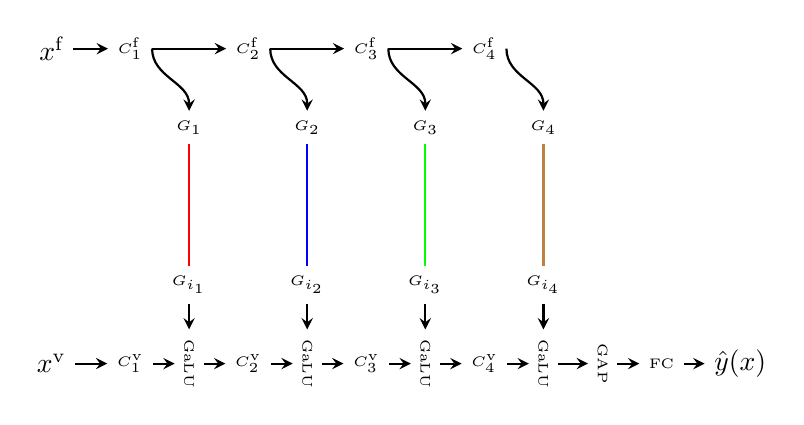
\begin{tikzpicture}
%\node []  (fntext)at (-4.625,-3.5) {CNN-GAP-DLGN};

%\node []  (output) at (7.5,1.5) {$\hat{y}(x)$};


\node [] (dgn1-f-c4) at (-3.5,1.5){\tiny{$C^{\text{f}}_4$}};
\node [] (dgn1-f-c3) at (-5,1.5){\tiny{$C^{\text{f}}_3$}};
\node [] (dgn1-f-c2) at (-6.5,1.5){\tiny{$C^{\text{f}}_2$}};
\node [] (dgn1-f-c1) at (-8,1.5){\tiny{$C^{\text{f}}_1$}};
\node [] (dgn1-input-f) at (-9,1.5){$x^{\text{f}}$};
\draw [-stealth,thick]   (dgn1-f-c3.east) -- (dgn1-f-c4.west);
\draw [-stealth,thick]   (dgn1-f-c2.east) -- (dgn1-f-c3.west);
\draw [-stealth,thick]   (dgn1-f-c1.east) -- (dgn1-f-c2.west);
\draw [-stealth,thick]   (dgn1-input-f.east) -- (dgn1-f-c1.west);



\node []  (dgn1-output) at (-0.25,-2.5) {$\hat{y}(x)$};

\node [] (dgn1-smax) at (-1.25,-2.5){\tiny{FC}};
\draw [-stealth,thick]   (dgn1-smax.east)--(dgn1-output.west);

\node [rotate=-90] (dgn1-gap) at (-2,-2.5){\tiny{GAP}};
\draw [-stealth,thick]   (dgn1-gap.north)--(dgn1-smax.west);


\node [rotate=-90] (dgn1-galu-4) at (-2.75,-2.5){\tiny{GaLU}};
\draw [-stealth,thick]   (dgn1-galu-4.north)--(dgn1-gap.south);

\node [] (dgn1-v-c4) at (-3.5,-2.5){\tiny{$C^{\text{v}}_4$}};
\draw [-stealth,thick]   (dgn1-v-c4.east) -- (dgn1-galu-4.south);


\node [rotate=-90] (dgn1-galu-3) at (-4.25,-2.5){\tiny{GaLU}};
\draw [-stealth,thick]   (dgn1-galu-3.north) -- (dgn1-v-c4.west);

\node [] (dgn1-v-c3) at (-5,-2.5){\tiny{$C^{\text{v}}_3$}};
\draw [-stealth,thick]   (dgn1-v-c3.east) -- (dgn1-galu-3.south);


\node [rotate=-90] (dgn1-galu-2) at (-5.75,-2.5){\tiny{GaLU}};
\draw [-stealth,thick]   (dgn1-galu-2.north) -- (dgn1-v-c3.west);

\node [] (dgn1-v-c2) at (-6.5,-2.5){\tiny{$C^{\text{v}}_2$}};
\draw [-stealth,thick]   (dgn1-v-c2.east) -- (dgn1-galu-2.south);


\node [rotate=-90] (dgn1-galu-1) at (-7.25,-2.5){\tiny{GaLU}};
\draw [-stealth,thick]   (dgn1-galu-1.north) -- (dgn1-v-c2.west);


\node [] (dgn1-v-c1) at (-8,-2.5){\tiny{$C^{\text{v}}_1$}};
\draw [-stealth,thick]   (dgn1-v-c1.east) -- (dgn1-galu-1.south);


\node [] (dgn1-v-input) at (-9,-2.5){$x^{\text{v}}$};

\draw [-stealth,thick]   (dgn1-v-input.east) -- (dgn1-v-c1.west);


\node[] (dgn1-gating-4-up) at (-2.75,0.5){\tiny{$G_{4}$}};
\draw [-stealth,thick]   (dgn1-f-c4.east) to[out=-90,in=90] (dgn1-gating-4-up.north);


\node[] (dgn1-gating-3-up) at (-4.25,0.5){\tiny{$G_{3}$}};
\draw [-stealth,thick]   (dgn1-f-c3.east) to[out=-90,in=90] (dgn1-gating-3-up.north);



\node[] (dgn1-gating-2-up) at (-5.75,0.5){\tiny{$G_{2}$}};
\draw [-stealth,thick]   (dgn1-f-c2.east) to[out=-90,in=90] (dgn1-gating-2-up.north);


\node[] (dgn1-gating-1-up) at (-7.25,0.5){\tiny{$G_{1}$}};
\draw [-stealth,thick]   (dgn1-f-c1.east) to[out=-90,in=90] (dgn1-gating-1-up.north);





\node[] (dgn1-gating-4) at (-2.75,-1.5){\tiny{$G_{i_4}$}};
\draw [-stealth,thick]   (dgn1-gating-4.south) -- (dgn1-galu-4.west);


\node[] (dgn1-gating-3) at (-4.25,-1.5){\tiny{$G_{i_3}$}};
\draw [-stealth,thick]   (dgn1-gating-3.south) -- (dgn1-galu-3.west);



\node[] (dgn1-gating-2) at (-5.75,-1.5){\tiny{$G_{i_2}$}};
\draw [-stealth,thick]   (dgn1-gating-2.south) -- (dgn1-galu-2.west);


\node[] (dgn1-gating-1) at (-7.25,-1.5){\tiny{$G_{i_1}$}};
\draw [-stealth,thick]   (dgn1-gating-1.south) -- (dgn1-galu-1.west);



\draw [-,thick,color=red]   (dgn1-gating-1-up.south) --(dgn1-gating-1.north);

\draw [-,thick,color=blue]   (dgn1-gating-2-up.south) --(dgn1-gating-2.north);

\draw [-,thick,color=green]   (dgn1-gating-3-up.south) --(dgn1-gating-3.north);

\draw [-,thick,color=brown]   (dgn1-gating-4-up.south) --(dgn1-gating-4.north);


%%%%%%%%%%%%%%%%%%%%%%%%%%%%%%%%%%%%%%%%%%%%%%%%%%%%%%%%%%%%%%%%%
	
\end{tikzpicture}


}
\end{minipage}
\begin{minipage}{0.48\columnwidth}
\centering
\resizebox{0.99\columnwidth}{!}{
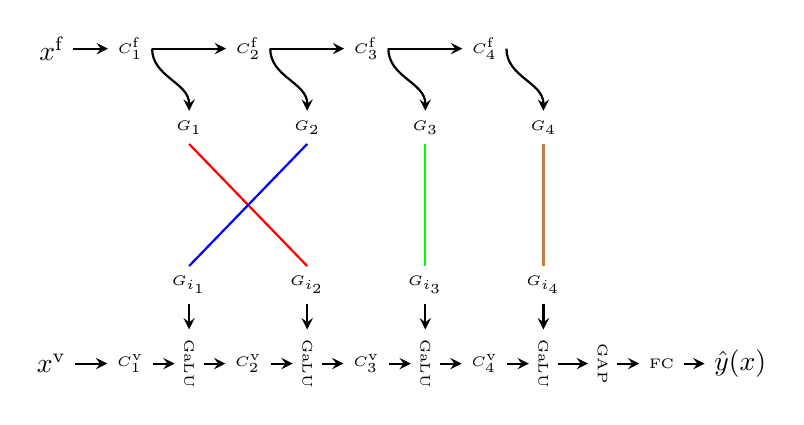
\begin{tikzpicture}
%\node []  (fntext)at (-4.625,-3.5) {CNN-GAP-DLGN};

%\node []  (output) at (7.5,1.5) {$\hat{y}(x)$};


\node [] (dgn1-f-c4) at (-3.5,1.5){\tiny{$C^{\text{f}}_4$}};
\node [] (dgn1-f-c3) at (-5,1.5){\tiny{$C^{\text{f}}_3$}};
\node [] (dgn1-f-c2) at (-6.5,1.5){\tiny{$C^{\text{f}}_2$}};
\node [] (dgn1-f-c1) at (-8,1.5){\tiny{$C^{\text{f}}_1$}};
\node [] (dgn1-input-f) at (-9,1.5){$x^{\text{f}}$};
\draw [-stealth,thick]   (dgn1-f-c3.east) -- (dgn1-f-c4.west);
\draw [-stealth,thick]   (dgn1-f-c2.east) -- (dgn1-f-c3.west);
\draw [-stealth,thick]   (dgn1-f-c1.east) -- (dgn1-f-c2.west);
\draw [-stealth,thick]   (dgn1-input-f.east) -- (dgn1-f-c1.west);



\node []  (dgn1-output) at (-0.25,-2.5) {$\hat{y}(x)$};

\node [] (dgn1-smax) at (-1.25,-2.5){\tiny{FC}};
\draw [-stealth,thick]   (dgn1-smax.east)--(dgn1-output.west);

\node [rotate=-90] (dgn1-gap) at (-2,-2.5){\tiny{GAP}};
\draw [-stealth,thick]   (dgn1-gap.north)--(dgn1-smax.west);


\node [rotate=-90] (dgn1-galu-4) at (-2.75,-2.5){\tiny{GaLU}};
\draw [-stealth,thick]   (dgn1-galu-4.north)--(dgn1-gap.south);

\node [] (dgn1-v-c4) at (-3.5,-2.5){\tiny{$C^{\text{v}}_4$}};
\draw [-stealth,thick]   (dgn1-v-c4.east) -- (dgn1-galu-4.south);


\node [rotate=-90] (dgn1-galu-3) at (-4.25,-2.5){\tiny{GaLU}};
\draw [-stealth,thick]   (dgn1-galu-3.north) -- (dgn1-v-c4.west);

\node [] (dgn1-v-c3) at (-5,-2.5){\tiny{$C^{\text{v}}_3$}};
\draw [-stealth,thick]   (dgn1-v-c3.east) -- (dgn1-galu-3.south);


\node [rotate=-90] (dgn1-galu-2) at (-5.75,-2.5){\tiny{GaLU}};
\draw [-stealth,thick]   (dgn1-galu-2.north) -- (dgn1-v-c3.west);

\node [] (dgn1-v-c2) at (-6.5,-2.5){\tiny{$C^{\text{v}}_2$}};
\draw [-stealth,thick]   (dgn1-v-c2.east) -- (dgn1-galu-2.south);


\node [rotate=-90] (dgn1-galu-1) at (-7.25,-2.5){\tiny{GaLU}};
\draw [-stealth,thick]   (dgn1-galu-1.north) -- (dgn1-v-c2.west);


\node [] (dgn1-v-c1) at (-8,-2.5){\tiny{$C^{\text{v}}_1$}};
\draw [-stealth,thick]   (dgn1-v-c1.east) -- (dgn1-galu-1.south);


\node [] (dgn1-v-input) at (-9,-2.5){$x^{\text{v}}$};

\draw [-stealth,thick]   (dgn1-v-input.east) -- (dgn1-v-c1.west);


\node[] (dgn1-gating-4-up) at (-2.75,0.5){\tiny{$G_{4}$}};
\draw [-stealth,thick]   (dgn1-f-c4.east) to[out=-90,in=90] (dgn1-gating-4-up.north);


\node[] (dgn1-gating-3-up) at (-4.25,0.5){\tiny{$G_{3}$}};
\draw [-stealth,thick]   (dgn1-f-c3.east) to[out=-90,in=90] (dgn1-gating-3-up.north);



\node[] (dgn1-gating-2-up) at (-5.75,0.5){\tiny{$G_{2}$}};
\draw [-stealth,thick]   (dgn1-f-c2.east) to[out=-90,in=90] (dgn1-gating-2-up.north);


\node[] (dgn1-gating-1-up) at (-7.25,0.5){\tiny{$G_{1}$}};
\draw [-stealth,thick]   (dgn1-f-c1.east) to[out=-90,in=90] (dgn1-gating-1-up.north);





\node[] (dgn1-gating-4) at (-2.75,-1.5){\tiny{$G_{i_4}$}};
\draw [-stealth,thick]   (dgn1-gating-4.south) -- (dgn1-galu-4.west);


\node[] (dgn1-gating-3) at (-4.25,-1.5){\tiny{$G_{i_3}$}};
\draw [-stealth,thick]   (dgn1-gating-3.south) -- (dgn1-galu-3.west);



\node[] (dgn1-gating-2) at (-5.75,-1.5){\tiny{$G_{i_2}$}};
\draw [-stealth,thick]   (dgn1-gating-2.south) -- (dgn1-galu-2.west);


\node[] (dgn1-gating-1) at (-7.25,-1.5){\tiny{$G_{i_1}$}};
\draw [-stealth,thick]   (dgn1-gating-1.south) -- (dgn1-galu-1.west);



\draw [-,thick,color=red]   (dgn1-gating-1-up.south) --(dgn1-gating-2.north);

\draw [-,thick,color=blue]   (dgn1-gating-2-up.south) --(dgn1-gating-1.north);

\draw [-,thick,color=green]   (dgn1-gating-3-up.south) --(dgn1-gating-3.north);

\draw [-,thick,color=brown]   (dgn1-gating-4-up.south) --(dgn1-gating-4.north);


%%%%%%%%%%%%%%%%%%%%%%%%%%%%%%%%%%%%%%%%%%%%%%%%%%%%%%%%%%%%%%%%%
	
\end{tikzpicture}


}
\end{minipage}

\begin{minipage}{0.48\columnwidth}
\centering
\resizebox{0.99\columnwidth}{!}{
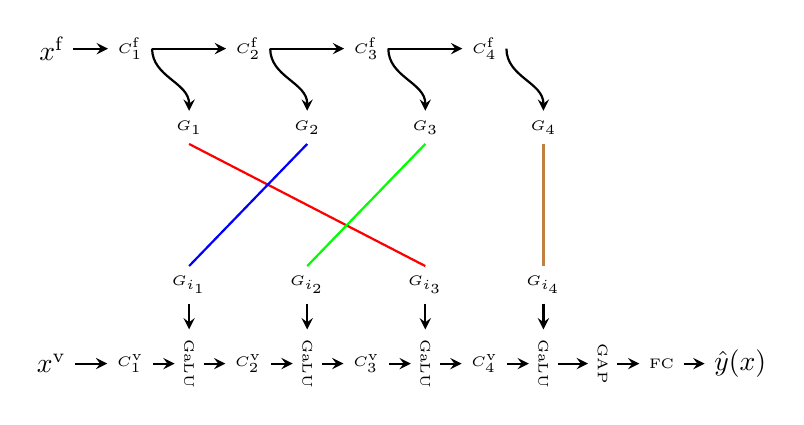
\begin{tikzpicture}
%\node []  (fntext)at (-4.625,-3.5) {CNN-GAP-DLGN};

%\node []  (output) at (7.5,1.5) {$\hat{y}(x)$};


\node [] (dgn1-f-c4) at (-3.5,1.5){\tiny{$C^{\text{f}}_4$}};
\node [] (dgn1-f-c3) at (-5,1.5){\tiny{$C^{\text{f}}_3$}};
\node [] (dgn1-f-c2) at (-6.5,1.5){\tiny{$C^{\text{f}}_2$}};
\node [] (dgn1-f-c1) at (-8,1.5){\tiny{$C^{\text{f}}_1$}};
\node [] (dgn1-input-f) at (-9,1.5){$x^{\text{f}}$};
\draw [-stealth,thick]   (dgn1-f-c3.east) -- (dgn1-f-c4.west);
\draw [-stealth,thick]   (dgn1-f-c2.east) -- (dgn1-f-c3.west);
\draw [-stealth,thick]   (dgn1-f-c1.east) -- (dgn1-f-c2.west);
\draw [-stealth,thick]   (dgn1-input-f.east) -- (dgn1-f-c1.west);



\node []  (dgn1-output) at (-0.25,-2.5) {$\hat{y}(x)$};

\node [] (dgn1-smax) at (-1.25,-2.5){\tiny{FC}};
\draw [-stealth,thick]   (dgn1-smax.east)--(dgn1-output.west);

\node [rotate=-90] (dgn1-gap) at (-2,-2.5){\tiny{GAP}};
\draw [-stealth,thick]   (dgn1-gap.north)--(dgn1-smax.west);


\node [rotate=-90] (dgn1-galu-4) at (-2.75,-2.5){\tiny{GaLU}};
\draw [-stealth,thick]   (dgn1-galu-4.north)--(dgn1-gap.south);

\node [] (dgn1-v-c4) at (-3.5,-2.5){\tiny{$C^{\text{v}}_4$}};
\draw [-stealth,thick]   (dgn1-v-c4.east) -- (dgn1-galu-4.south);


\node [rotate=-90] (dgn1-galu-3) at (-4.25,-2.5){\tiny{GaLU}};
\draw [-stealth,thick]   (dgn1-galu-3.north) -- (dgn1-v-c4.west);

\node [] (dgn1-v-c3) at (-5,-2.5){\tiny{$C^{\text{v}}_3$}};
\draw [-stealth,thick]   (dgn1-v-c3.east) -- (dgn1-galu-3.south);


\node [rotate=-90] (dgn1-galu-2) at (-5.75,-2.5){\tiny{GaLU}};
\draw [-stealth,thick]   (dgn1-galu-2.north) -- (dgn1-v-c3.west);

\node [] (dgn1-v-c2) at (-6.5,-2.5){\tiny{$C^{\text{v}}_2$}};
\draw [-stealth,thick]   (dgn1-v-c2.east) -- (dgn1-galu-2.south);


\node [rotate=-90] (dgn1-galu-1) at (-7.25,-2.5){\tiny{GaLU}};
\draw [-stealth,thick]   (dgn1-galu-1.north) -- (dgn1-v-c2.west);


\node [] (dgn1-v-c1) at (-8,-2.5){\tiny{$C^{\text{v}}_1$}};
\draw [-stealth,thick]   (dgn1-v-c1.east) -- (dgn1-galu-1.south);


\node [] (dgn1-v-input) at (-9,-2.5){$x^{\text{v}}$};

\draw [-stealth,thick]   (dgn1-v-input.east) -- (dgn1-v-c1.west);


\node[] (dgn1-gating-4-up) at (-2.75,0.5){\tiny{$G_{4}$}};
\draw [-stealth,thick]   (dgn1-f-c4.east) to[out=-90,in=90] (dgn1-gating-4-up.north);


\node[] (dgn1-gating-3-up) at (-4.25,0.5){\tiny{$G_{3}$}};
\draw [-stealth,thick]   (dgn1-f-c3.east) to[out=-90,in=90] (dgn1-gating-3-up.north);



\node[] (dgn1-gating-2-up) at (-5.75,0.5){\tiny{$G_{2}$}};
\draw [-stealth,thick]   (dgn1-f-c2.east) to[out=-90,in=90] (dgn1-gating-2-up.north);


\node[] (dgn1-gating-1-up) at (-7.25,0.5){\tiny{$G_{1}$}};
\draw [-stealth,thick]   (dgn1-f-c1.east) to[out=-90,in=90] (dgn1-gating-1-up.north);





\node[] (dgn1-gating-4) at (-2.75,-1.5){\tiny{$G_{i_4}$}};
\draw [-stealth,thick]   (dgn1-gating-4.south) -- (dgn1-galu-4.west);


\node[] (dgn1-gating-3) at (-4.25,-1.5){\tiny{$G_{i_3}$}};
\draw [-stealth,thick]   (dgn1-gating-3.south) -- (dgn1-galu-3.west);



\node[] (dgn1-gating-2) at (-5.75,-1.5){\tiny{$G_{i_2}$}};
\draw [-stealth,thick]   (dgn1-gating-2.south) -- (dgn1-galu-2.west);


\node[] (dgn1-gating-1) at (-7.25,-1.5){\tiny{$G_{i_1}$}};
\draw [-stealth,thick]   (dgn1-gating-1.south) -- (dgn1-galu-1.west);



\draw [-,thick,color=red]   (dgn1-gating-1-up.south) --(dgn1-gating-3.north);

\draw [-,thick,color=blue]   (dgn1-gating-2-up.south) --(dgn1-gating-1.north);

\draw [-,thick,color=green]   (dgn1-gating-3-up.south) --(dgn1-gating-2.north);

\draw [-,thick,color=brown]   (dgn1-gating-4-up.south) --(dgn1-gating-4.north);


%%%%%%%%%%%%%%%%%%%%%%%%%%%%%%%%%%%%%%%%%%%%%%%%%%%%%%%%%%%%%%%%%
	
\end{tikzpicture}


}
\end{minipage}
\begin{minipage}{0.48\columnwidth}
\centering
\resizebox{0.99\columnwidth}{!}{
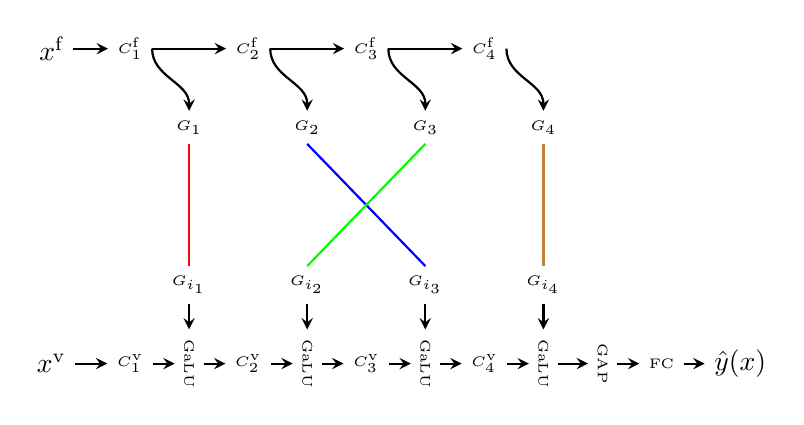
\begin{tikzpicture}
%\node []  (fntext)at (-4.625,-3.5) {CNN-GAP-DLGN};

%\node []  (output) at (7.5,1.5) {$\hat{y}(x)$};


\node [] (dgn1-f-c4) at (-3.5,1.5){\tiny{$C^{\text{f}}_4$}};
\node [] (dgn1-f-c3) at (-5,1.5){\tiny{$C^{\text{f}}_3$}};
\node [] (dgn1-f-c2) at (-6.5,1.5){\tiny{$C^{\text{f}}_2$}};
\node [] (dgn1-f-c1) at (-8,1.5){\tiny{$C^{\text{f}}_1$}};
\node [] (dgn1-input-f) at (-9,1.5){$x^{\text{f}}$};
\draw [-stealth,thick]   (dgn1-f-c3.east) -- (dgn1-f-c4.west);
\draw [-stealth,thick]   (dgn1-f-c2.east) -- (dgn1-f-c3.west);
\draw [-stealth,thick]   (dgn1-f-c1.east) -- (dgn1-f-c2.west);
\draw [-stealth,thick]   (dgn1-input-f.east) -- (dgn1-f-c1.west);



\node []  (dgn1-output) at (-0.25,-2.5) {$\hat{y}(x)$};

\node [] (dgn1-smax) at (-1.25,-2.5){\tiny{FC}};
\draw [-stealth,thick]   (dgn1-smax.east)--(dgn1-output.west);

\node [rotate=-90] (dgn1-gap) at (-2,-2.5){\tiny{GAP}};
\draw [-stealth,thick]   (dgn1-gap.north)--(dgn1-smax.west);


\node [rotate=-90] (dgn1-galu-4) at (-2.75,-2.5){\tiny{GaLU}};
\draw [-stealth,thick]   (dgn1-galu-4.north)--(dgn1-gap.south);

\node [] (dgn1-v-c4) at (-3.5,-2.5){\tiny{$C^{\text{v}}_4$}};
\draw [-stealth,thick]   (dgn1-v-c4.east) -- (dgn1-galu-4.south);


\node [rotate=-90] (dgn1-galu-3) at (-4.25,-2.5){\tiny{GaLU}};
\draw [-stealth,thick]   (dgn1-galu-3.north) -- (dgn1-v-c4.west);

\node [] (dgn1-v-c3) at (-5,-2.5){\tiny{$C^{\text{v}}_3$}};
\draw [-stealth,thick]   (dgn1-v-c3.east) -- (dgn1-galu-3.south);


\node [rotate=-90] (dgn1-galu-2) at (-5.75,-2.5){\tiny{GaLU}};
\draw [-stealth,thick]   (dgn1-galu-2.north) -- (dgn1-v-c3.west);

\node [] (dgn1-v-c2) at (-6.5,-2.5){\tiny{$C^{\text{v}}_2$}};
\draw [-stealth,thick]   (dgn1-v-c2.east) -- (dgn1-galu-2.south);


\node [rotate=-90] (dgn1-galu-1) at (-7.25,-2.5){\tiny{GaLU}};
\draw [-stealth,thick]   (dgn1-galu-1.north) -- (dgn1-v-c2.west);


\node [] (dgn1-v-c1) at (-8,-2.5){\tiny{$C^{\text{v}}_1$}};
\draw [-stealth,thick]   (dgn1-v-c1.east) -- (dgn1-galu-1.south);


\node [] (dgn1-v-input) at (-9,-2.5){$x^{\text{v}}$};

\draw [-stealth,thick]   (dgn1-v-input.east) -- (dgn1-v-c1.west);


\node[] (dgn1-gating-4-up) at (-2.75,0.5){\tiny{$G_{4}$}};
\draw [-stealth,thick]   (dgn1-f-c4.east) to[out=-90,in=90] (dgn1-gating-4-up.north);


\node[] (dgn1-gating-3-up) at (-4.25,0.5){\tiny{$G_{3}$}};
\draw [-stealth,thick]   (dgn1-f-c3.east) to[out=-90,in=90] (dgn1-gating-3-up.north);



\node[] (dgn1-gating-2-up) at (-5.75,0.5){\tiny{$G_{2}$}};
\draw [-stealth,thick]   (dgn1-f-c2.east) to[out=-90,in=90] (dgn1-gating-2-up.north);


\node[] (dgn1-gating-1-up) at (-7.25,0.5){\tiny{$G_{1}$}};
\draw [-stealth,thick]   (dgn1-f-c1.east) to[out=-90,in=90] (dgn1-gating-1-up.north);





\node[] (dgn1-gating-4) at (-2.75,-1.5){\tiny{$G_{i_4}$}};
\draw [-stealth,thick]   (dgn1-gating-4.south) -- (dgn1-galu-4.west);


\node[] (dgn1-gating-3) at (-4.25,-1.5){\tiny{$G_{i_3}$}};
\draw [-stealth,thick]   (dgn1-gating-3.south) -- (dgn1-galu-3.west);



\node[] (dgn1-gating-2) at (-5.75,-1.5){\tiny{$G_{i_2}$}};
\draw [-stealth,thick]   (dgn1-gating-2.south) -- (dgn1-galu-2.west);


\node[] (dgn1-gating-1) at (-7.25,-1.5){\tiny{$G_{i_1}$}};
\draw [-stealth,thick]   (dgn1-gating-1.south) -- (dgn1-galu-1.west);



\draw [-,thick,color=red]   (dgn1-gating-1-up.south) --(dgn1-gating-1.north);

\draw [-,thick,color=blue]   (dgn1-gating-2-up.south) --(dgn1-gating-3.north);

\draw [-,thick,color=green]   (dgn1-gating-3-up.south) --(dgn1-gating-2.north);

\draw [-,thick,color=brown]   (dgn1-gating-4-up.south) --(dgn1-gating-4.north);


%%%%%%%%%%%%%%%%%%%%%%%%%%%%%%%%%%%%%%%%%%%%%%%%%%%%%%%%%%%%%%%%%
	
\end{tikzpicture}


}
\end{minipage}


\begin{minipage}{0.48\columnwidth}
\centering
\resizebox{0.99\columnwidth}{!}{
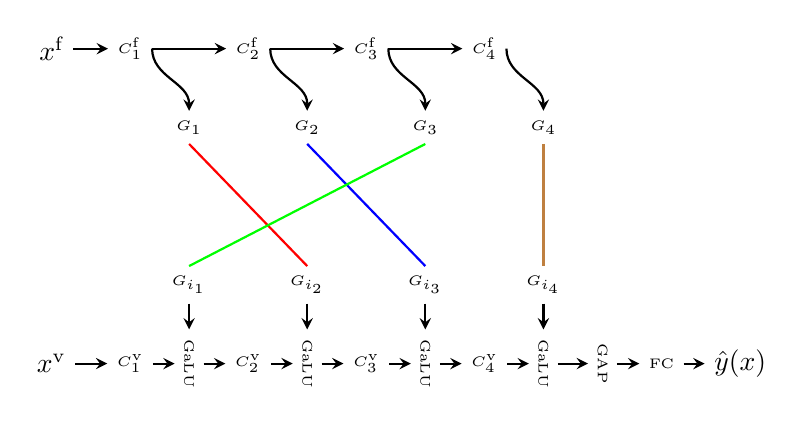
\begin{tikzpicture}
%\node []  (fntext)at (-4.625,-3.5) {CNN-GAP-DLGN};

%\node []  (output) at (7.5,1.5) {$\hat{y}(x)$};


\node [] (dgn1-f-c4) at (-3.5,1.5){\tiny{$C^{\text{f}}_4$}};
\node [] (dgn1-f-c3) at (-5,1.5){\tiny{$C^{\text{f}}_3$}};
\node [] (dgn1-f-c2) at (-6.5,1.5){\tiny{$C^{\text{f}}_2$}};
\node [] (dgn1-f-c1) at (-8,1.5){\tiny{$C^{\text{f}}_1$}};
\node [] (dgn1-input-f) at (-9,1.5){$x^{\text{f}}$};
\draw [-stealth,thick]   (dgn1-f-c3.east) -- (dgn1-f-c4.west);
\draw [-stealth,thick]   (dgn1-f-c2.east) -- (dgn1-f-c3.west);
\draw [-stealth,thick]   (dgn1-f-c1.east) -- (dgn1-f-c2.west);
\draw [-stealth,thick]   (dgn1-input-f.east) -- (dgn1-f-c1.west);



\node []  (dgn1-output) at (-0.25,-2.5) {$\hat{y}(x)$};

\node [] (dgn1-smax) at (-1.25,-2.5){\tiny{FC}};
\draw [-stealth,thick]   (dgn1-smax.east)--(dgn1-output.west);

\node [rotate=-90] (dgn1-gap) at (-2,-2.5){\tiny{GAP}};
\draw [-stealth,thick]   (dgn1-gap.north)--(dgn1-smax.west);


\node [rotate=-90] (dgn1-galu-4) at (-2.75,-2.5){\tiny{GaLU}};
\draw [-stealth,thick]   (dgn1-galu-4.north)--(dgn1-gap.south);

\node [] (dgn1-v-c4) at (-3.5,-2.5){\tiny{$C^{\text{v}}_4$}};
\draw [-stealth,thick]   (dgn1-v-c4.east) -- (dgn1-galu-4.south);


\node [rotate=-90] (dgn1-galu-3) at (-4.25,-2.5){\tiny{GaLU}};
\draw [-stealth,thick]   (dgn1-galu-3.north) -- (dgn1-v-c4.west);

\node [] (dgn1-v-c3) at (-5,-2.5){\tiny{$C^{\text{v}}_3$}};
\draw [-stealth,thick]   (dgn1-v-c3.east) -- (dgn1-galu-3.south);


\node [rotate=-90] (dgn1-galu-2) at (-5.75,-2.5){\tiny{GaLU}};
\draw [-stealth,thick]   (dgn1-galu-2.north) -- (dgn1-v-c3.west);

\node [] (dgn1-v-c2) at (-6.5,-2.5){\tiny{$C^{\text{v}}_2$}};
\draw [-stealth,thick]   (dgn1-v-c2.east) -- (dgn1-galu-2.south);


\node [rotate=-90] (dgn1-galu-1) at (-7.25,-2.5){\tiny{GaLU}};
\draw [-stealth,thick]   (dgn1-galu-1.north) -- (dgn1-v-c2.west);


\node [] (dgn1-v-c1) at (-8,-2.5){\tiny{$C^{\text{v}}_1$}};
\draw [-stealth,thick]   (dgn1-v-c1.east) -- (dgn1-galu-1.south);


\node [] (dgn1-v-input) at (-9,-2.5){$x^{\text{v}}$};

\draw [-stealth,thick]   (dgn1-v-input.east) -- (dgn1-v-c1.west);


\node[] (dgn1-gating-4-up) at (-2.75,0.5){\tiny{$G_{4}$}};
\draw [-stealth,thick]   (dgn1-f-c4.east) to[out=-90,in=90] (dgn1-gating-4-up.north);


\node[] (dgn1-gating-3-up) at (-4.25,0.5){\tiny{$G_{3}$}};
\draw [-stealth,thick]   (dgn1-f-c3.east) to[out=-90,in=90] (dgn1-gating-3-up.north);



\node[] (dgn1-gating-2-up) at (-5.75,0.5){\tiny{$G_{2}$}};
\draw [-stealth,thick]   (dgn1-f-c2.east) to[out=-90,in=90] (dgn1-gating-2-up.north);


\node[] (dgn1-gating-1-up) at (-7.25,0.5){\tiny{$G_{1}$}};
\draw [-stealth,thick]   (dgn1-f-c1.east) to[out=-90,in=90] (dgn1-gating-1-up.north);





\node[] (dgn1-gating-4) at (-2.75,-1.5){\tiny{$G_{i_4}$}};
\draw [-stealth,thick]   (dgn1-gating-4.south) -- (dgn1-galu-4.west);


\node[] (dgn1-gating-3) at (-4.25,-1.5){\tiny{$G_{i_3}$}};
\draw [-stealth,thick]   (dgn1-gating-3.south) -- (dgn1-galu-3.west);



\node[] (dgn1-gating-2) at (-5.75,-1.5){\tiny{$G_{i_2}$}};
\draw [-stealth,thick]   (dgn1-gating-2.south) -- (dgn1-galu-2.west);


\node[] (dgn1-gating-1) at (-7.25,-1.5){\tiny{$G_{i_1}$}};
\draw [-stealth,thick]   (dgn1-gating-1.south) -- (dgn1-galu-1.west);



\draw [-,thick,color=red]   (dgn1-gating-1-up.south) --(dgn1-gating-2.north);

\draw [-,thick,color=blue]   (dgn1-gating-2-up.south) --(dgn1-gating-3.north);

\draw [-,thick,color=green]   (dgn1-gating-3-up.south) --(dgn1-gating-1.north);

\draw [-,thick,color=brown]   (dgn1-gating-4-up.south) --(dgn1-gating-4.north);


%%%%%%%%%%%%%%%%%%%%%%%%%%%%%%%%%%%%%%%%%%%%%%%%%%%%%%%%%%%%%%%%%
	
\end{tikzpicture}


}
\end{minipage}
\begin{minipage}{0.48\columnwidth}
\centering
\resizebox{0.99\columnwidth}{!}{
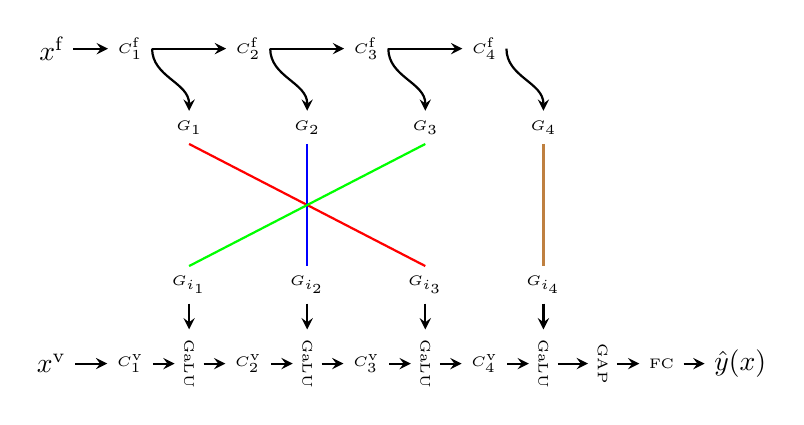
\begin{tikzpicture}
%\node []  (fntext)at (-4.625,-3.5) {CNN-GAP-DLGN};

%\node []  (output) at (7.5,1.5) {$\hat{y}(x)$};


\node [] (dgn1-f-c4) at (-3.5,1.5){\tiny{$C^{\text{f}}_4$}};
\node [] (dgn1-f-c3) at (-5,1.5){\tiny{$C^{\text{f}}_3$}};
\node [] (dgn1-f-c2) at (-6.5,1.5){\tiny{$C^{\text{f}}_2$}};
\node [] (dgn1-f-c1) at (-8,1.5){\tiny{$C^{\text{f}}_1$}};
\node [] (dgn1-input-f) at (-9,1.5){$x^{\text{f}}$};
\draw [-stealth,thick]   (dgn1-f-c3.east) -- (dgn1-f-c4.west);
\draw [-stealth,thick]   (dgn1-f-c2.east) -- (dgn1-f-c3.west);
\draw [-stealth,thick]   (dgn1-f-c1.east) -- (dgn1-f-c2.west);
\draw [-stealth,thick]   (dgn1-input-f.east) -- (dgn1-f-c1.west);



\node []  (dgn1-output) at (-0.25,-2.5) {$\hat{y}(x)$};

\node [] (dgn1-smax) at (-1.25,-2.5){\tiny{FC}};
\draw [-stealth,thick]   (dgn1-smax.east)--(dgn1-output.west);

\node [rotate=-90] (dgn1-gap) at (-2,-2.5){\tiny{GAP}};
\draw [-stealth,thick]   (dgn1-gap.north)--(dgn1-smax.west);


\node [rotate=-90] (dgn1-galu-4) at (-2.75,-2.5){\tiny{GaLU}};
\draw [-stealth,thick]   (dgn1-galu-4.north)--(dgn1-gap.south);

\node [] (dgn1-v-c4) at (-3.5,-2.5){\tiny{$C^{\text{v}}_4$}};
\draw [-stealth,thick]   (dgn1-v-c4.east) -- (dgn1-galu-4.south);


\node [rotate=-90] (dgn1-galu-3) at (-4.25,-2.5){\tiny{GaLU}};
\draw [-stealth,thick]   (dgn1-galu-3.north) -- (dgn1-v-c4.west);

\node [] (dgn1-v-c3) at (-5,-2.5){\tiny{$C^{\text{v}}_3$}};
\draw [-stealth,thick]   (dgn1-v-c3.east) -- (dgn1-galu-3.south);


\node [rotate=-90] (dgn1-galu-2) at (-5.75,-2.5){\tiny{GaLU}};
\draw [-stealth,thick]   (dgn1-galu-2.north) -- (dgn1-v-c3.west);

\node [] (dgn1-v-c2) at (-6.5,-2.5){\tiny{$C^{\text{v}}_2$}};
\draw [-stealth,thick]   (dgn1-v-c2.east) -- (dgn1-galu-2.south);


\node [rotate=-90] (dgn1-galu-1) at (-7.25,-2.5){\tiny{GaLU}};
\draw [-stealth,thick]   (dgn1-galu-1.north) -- (dgn1-v-c2.west);


\node [] (dgn1-v-c1) at (-8,-2.5){\tiny{$C^{\text{v}}_1$}};
\draw [-stealth,thick]   (dgn1-v-c1.east) -- (dgn1-galu-1.south);


\node [] (dgn1-v-input) at (-9,-2.5){$x^{\text{v}}$};

\draw [-stealth,thick]   (dgn1-v-input.east) -- (dgn1-v-c1.west);


\node[] (dgn1-gating-4-up) at (-2.75,0.5){\tiny{$G_{4}$}};
\draw [-stealth,thick]   (dgn1-f-c4.east) to[out=-90,in=90] (dgn1-gating-4-up.north);


\node[] (dgn1-gating-3-up) at (-4.25,0.5){\tiny{$G_{3}$}};
\draw [-stealth,thick]   (dgn1-f-c3.east) to[out=-90,in=90] (dgn1-gating-3-up.north);



\node[] (dgn1-gating-2-up) at (-5.75,0.5){\tiny{$G_{2}$}};
\draw [-stealth,thick]   (dgn1-f-c2.east) to[out=-90,in=90] (dgn1-gating-2-up.north);


\node[] (dgn1-gating-1-up) at (-7.25,0.5){\tiny{$G_{1}$}};
\draw [-stealth,thick]   (dgn1-f-c1.east) to[out=-90,in=90] (dgn1-gating-1-up.north);





\node[] (dgn1-gating-4) at (-2.75,-1.5){\tiny{$G_{i_4}$}};
\draw [-stealth,thick]   (dgn1-gating-4.south) -- (dgn1-galu-4.west);


\node[] (dgn1-gating-3) at (-4.25,-1.5){\tiny{$G_{i_3}$}};
\draw [-stealth,thick]   (dgn1-gating-3.south) -- (dgn1-galu-3.west);



\node[] (dgn1-gating-2) at (-5.75,-1.5){\tiny{$G_{i_2}$}};
\draw [-stealth,thick]   (dgn1-gating-2.south) -- (dgn1-galu-2.west);


\node[] (dgn1-gating-1) at (-7.25,-1.5){\tiny{$G_{i_1}$}};
\draw [-stealth,thick]   (dgn1-gating-1.south) -- (dgn1-galu-1.west);



\draw [-,thick,color=red]   (dgn1-gating-1-up.south) --(dgn1-gating-3.north);

\draw [-,thick,color=blue]   (dgn1-gating-2-up.south) --(dgn1-gating-2.north);

\draw [-,thick,color=green]   (dgn1-gating-3-up.south) --(dgn1-gating-1.north);

\draw [-,thick,color=brown]   (dgn1-gating-4-up.south) --(dgn1-gating-4.north);


%%%%%%%%%%%%%%%%%%%%%%%%%%%%%%%%%%%%%%%%%%%%%%%%%%%%%%%%%%%%%%%%%
	
\end{tikzpicture}


}
\end{minipage}



\begin{minipage}{0.48\columnwidth}
\centering
\resizebox{0.99\columnwidth}{!}{
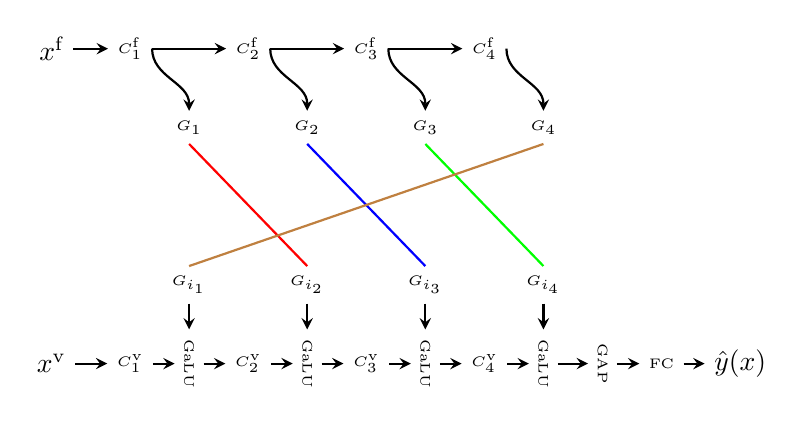
\begin{tikzpicture}
%\node []  (fntext)at (-4.625,-3.5) {CNN-GAP-DLGN};

%\node []  (output) at (7.5,1.5) {$\hat{y}(x)$};


\node [] (dgn1-f-c4) at (-3.5,1.5){\tiny{$C^{\text{f}}_4$}};
\node [] (dgn1-f-c3) at (-5,1.5){\tiny{$C^{\text{f}}_3$}};
\node [] (dgn1-f-c2) at (-6.5,1.5){\tiny{$C^{\text{f}}_2$}};
\node [] (dgn1-f-c1) at (-8,1.5){\tiny{$C^{\text{f}}_1$}};
\node [] (dgn1-input-f) at (-9,1.5){$x^{\text{f}}$};
\draw [-stealth,thick]   (dgn1-f-c3.east) -- (dgn1-f-c4.west);
\draw [-stealth,thick]   (dgn1-f-c2.east) -- (dgn1-f-c3.west);
\draw [-stealth,thick]   (dgn1-f-c1.east) -- (dgn1-f-c2.west);
\draw [-stealth,thick]   (dgn1-input-f.east) -- (dgn1-f-c1.west);



\node []  (dgn1-output) at (-0.25,-2.5) {$\hat{y}(x)$};

\node [] (dgn1-smax) at (-1.25,-2.5){\tiny{FC}};
\draw [-stealth,thick]   (dgn1-smax.east)--(dgn1-output.west);

\node [rotate=-90] (dgn1-gap) at (-2,-2.5){\tiny{GAP}};
\draw [-stealth,thick]   (dgn1-gap.north)--(dgn1-smax.west);


\node [rotate=-90] (dgn1-galu-4) at (-2.75,-2.5){\tiny{GaLU}};
\draw [-stealth,thick]   (dgn1-galu-4.north)--(dgn1-gap.south);

\node [] (dgn1-v-c4) at (-3.5,-2.5){\tiny{$C^{\text{v}}_4$}};
\draw [-stealth,thick]   (dgn1-v-c4.east) -- (dgn1-galu-4.south);


\node [rotate=-90] (dgn1-galu-3) at (-4.25,-2.5){\tiny{GaLU}};
\draw [-stealth,thick]   (dgn1-galu-3.north) -- (dgn1-v-c4.west);

\node [] (dgn1-v-c3) at (-5,-2.5){\tiny{$C^{\text{v}}_3$}};
\draw [-stealth,thick]   (dgn1-v-c3.east) -- (dgn1-galu-3.south);


\node [rotate=-90] (dgn1-galu-2) at (-5.75,-2.5){\tiny{GaLU}};
\draw [-stealth,thick]   (dgn1-galu-2.north) -- (dgn1-v-c3.west);

\node [] (dgn1-v-c2) at (-6.5,-2.5){\tiny{$C^{\text{v}}_2$}};
\draw [-stealth,thick]   (dgn1-v-c2.east) -- (dgn1-galu-2.south);


\node [rotate=-90] (dgn1-galu-1) at (-7.25,-2.5){\tiny{GaLU}};
\draw [-stealth,thick]   (dgn1-galu-1.north) -- (dgn1-v-c2.west);


\node [] (dgn1-v-c1) at (-8,-2.5){\tiny{$C^{\text{v}}_1$}};
\draw [-stealth,thick]   (dgn1-v-c1.east) -- (dgn1-galu-1.south);


\node [] (dgn1-v-input) at (-9,-2.5){$x^{\text{v}}$};

\draw [-stealth,thick]   (dgn1-v-input.east) -- (dgn1-v-c1.west);


\node[] (dgn1-gating-4-up) at (-2.75,0.5){\tiny{$G_{4}$}};
\draw [-stealth,thick]   (dgn1-f-c4.east) to[out=-90,in=90] (dgn1-gating-4-up.north);


\node[] (dgn1-gating-3-up) at (-4.25,0.5){\tiny{$G_{3}$}};
\draw [-stealth,thick]   (dgn1-f-c3.east) to[out=-90,in=90] (dgn1-gating-3-up.north);



\node[] (dgn1-gating-2-up) at (-5.75,0.5){\tiny{$G_{2}$}};
\draw [-stealth,thick]   (dgn1-f-c2.east) to[out=-90,in=90] (dgn1-gating-2-up.north);


\node[] (dgn1-gating-1-up) at (-7.25,0.5){\tiny{$G_{1}$}};
\draw [-stealth,thick]   (dgn1-f-c1.east) to[out=-90,in=90] (dgn1-gating-1-up.north);





\node[] (dgn1-gating-4) at (-2.75,-1.5){\tiny{$G_{i_4}$}};
\draw [-stealth,thick]   (dgn1-gating-4.south) -- (dgn1-galu-4.west);


\node[] (dgn1-gating-3) at (-4.25,-1.5){\tiny{$G_{i_3}$}};
\draw [-stealth,thick]   (dgn1-gating-3.south) -- (dgn1-galu-3.west);



\node[] (dgn1-gating-2) at (-5.75,-1.5){\tiny{$G_{i_2}$}};
\draw [-stealth,thick]   (dgn1-gating-2.south) -- (dgn1-galu-2.west);


\node[] (dgn1-gating-1) at (-7.25,-1.5){\tiny{$G_{i_1}$}};
\draw [-stealth,thick]   (dgn1-gating-1.south) -- (dgn1-galu-1.west);



\draw [-,thick,color=red]   (dgn1-gating-1-up.south) --(dgn1-gating-2.north);

\draw [-,thick,color=blue]   (dgn1-gating-2-up.south) --(dgn1-gating-3.north);

\draw [-,thick,color=green]   (dgn1-gating-3-up.south) --(dgn1-gating-4.north);

\draw [-,thick,color=brown]   (dgn1-gating-4-up.south) --(dgn1-gating-1.north);


%%%%%%%%%%%%%%%%%%%%%%%%%%%%%%%%%%%%%%%%%%%%%%%%%%%%%%%%%%%%%%%%%
	
\end{tikzpicture}


}
\end{minipage}
\begin{minipage}{0.48\columnwidth}
\centering
\resizebox{0.99\columnwidth}{!}{
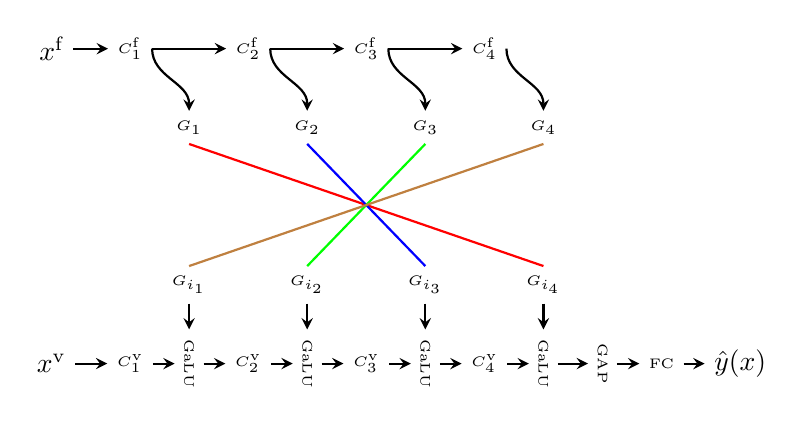
\begin{tikzpicture}
%\node []  (fntext)at (-4.625,-3.5) {CNN-GAP-DLGN};

%\node []  (output) at (7.5,1.5) {$\hat{y}(x)$};


\node [] (dgn1-f-c4) at (-3.5,1.5){\tiny{$C^{\text{f}}_4$}};
\node [] (dgn1-f-c3) at (-5,1.5){\tiny{$C^{\text{f}}_3$}};
\node [] (dgn1-f-c2) at (-6.5,1.5){\tiny{$C^{\text{f}}_2$}};
\node [] (dgn1-f-c1) at (-8,1.5){\tiny{$C^{\text{f}}_1$}};
\node [] (dgn1-input-f) at (-9,1.5){$x^{\text{f}}$};
\draw [-stealth,thick]   (dgn1-f-c3.east) -- (dgn1-f-c4.west);
\draw [-stealth,thick]   (dgn1-f-c2.east) -- (dgn1-f-c3.west);
\draw [-stealth,thick]   (dgn1-f-c1.east) -- (dgn1-f-c2.west);
\draw [-stealth,thick]   (dgn1-input-f.east) -- (dgn1-f-c1.west);



\node []  (dgn1-output) at (-0.25,-2.5) {$\hat{y}(x)$};

\node [] (dgn1-smax) at (-1.25,-2.5){\tiny{FC}};
\draw [-stealth,thick]   (dgn1-smax.east)--(dgn1-output.west);

\node [rotate=-90] (dgn1-gap) at (-2,-2.5){\tiny{GAP}};
\draw [-stealth,thick]   (dgn1-gap.north)--(dgn1-smax.west);


\node [rotate=-90] (dgn1-galu-4) at (-2.75,-2.5){\tiny{GaLU}};
\draw [-stealth,thick]   (dgn1-galu-4.north)--(dgn1-gap.south);

\node [] (dgn1-v-c4) at (-3.5,-2.5){\tiny{$C^{\text{v}}_4$}};
\draw [-stealth,thick]   (dgn1-v-c4.east) -- (dgn1-galu-4.south);


\node [rotate=-90] (dgn1-galu-3) at (-4.25,-2.5){\tiny{GaLU}};
\draw [-stealth,thick]   (dgn1-galu-3.north) -- (dgn1-v-c4.west);

\node [] (dgn1-v-c3) at (-5,-2.5){\tiny{$C^{\text{v}}_3$}};
\draw [-stealth,thick]   (dgn1-v-c3.east) -- (dgn1-galu-3.south);


\node [rotate=-90] (dgn1-galu-2) at (-5.75,-2.5){\tiny{GaLU}};
\draw [-stealth,thick]   (dgn1-galu-2.north) -- (dgn1-v-c3.west);

\node [] (dgn1-v-c2) at (-6.5,-2.5){\tiny{$C^{\text{v}}_2$}};
\draw [-stealth,thick]   (dgn1-v-c2.east) -- (dgn1-galu-2.south);


\node [rotate=-90] (dgn1-galu-1) at (-7.25,-2.5){\tiny{GaLU}};
\draw [-stealth,thick]   (dgn1-galu-1.north) -- (dgn1-v-c2.west);


\node [] (dgn1-v-c1) at (-8,-2.5){\tiny{$C^{\text{v}}_1$}};
\draw [-stealth,thick]   (dgn1-v-c1.east) -- (dgn1-galu-1.south);


\node [] (dgn1-v-input) at (-9,-2.5){$x^{\text{v}}$};

\draw [-stealth,thick]   (dgn1-v-input.east) -- (dgn1-v-c1.west);


\node[] (dgn1-gating-4-up) at (-2.75,0.5){\tiny{$G_{4}$}};
\draw [-stealth,thick]   (dgn1-f-c4.east) to[out=-90,in=90] (dgn1-gating-4-up.north);


\node[] (dgn1-gating-3-up) at (-4.25,0.5){\tiny{$G_{3}$}};
\draw [-stealth,thick]   (dgn1-f-c3.east) to[out=-90,in=90] (dgn1-gating-3-up.north);



\node[] (dgn1-gating-2-up) at (-5.75,0.5){\tiny{$G_{2}$}};
\draw [-stealth,thick]   (dgn1-f-c2.east) to[out=-90,in=90] (dgn1-gating-2-up.north);


\node[] (dgn1-gating-1-up) at (-7.25,0.5){\tiny{$G_{1}$}};
\draw [-stealth,thick]   (dgn1-f-c1.east) to[out=-90,in=90] (dgn1-gating-1-up.north);





\node[] (dgn1-gating-4) at (-2.75,-1.5){\tiny{$G_{i_4}$}};
\draw [-stealth,thick]   (dgn1-gating-4.south) -- (dgn1-galu-4.west);


\node[] (dgn1-gating-3) at (-4.25,-1.5){\tiny{$G_{i_3}$}};
\draw [-stealth,thick]   (dgn1-gating-3.south) -- (dgn1-galu-3.west);



\node[] (dgn1-gating-2) at (-5.75,-1.5){\tiny{$G_{i_2}$}};
\draw [-stealth,thick]   (dgn1-gating-2.south) -- (dgn1-galu-2.west);


\node[] (dgn1-gating-1) at (-7.25,-1.5){\tiny{$G_{i_1}$}};
\draw [-stealth,thick]   (dgn1-gating-1.south) -- (dgn1-galu-1.west);



\draw [-,thick,color=red]   (dgn1-gating-1-up.south) --(dgn1-gating-4.north);

\draw [-,thick,color=blue]   (dgn1-gating-2-up.south) --(dgn1-gating-3.north);

\draw [-,thick,color=green]   (dgn1-gating-3-up.south) --(dgn1-gating-2.north);

\draw [-,thick,color=brown]   (dgn1-gating-4-up.south) --(dgn1-gating-1.north);


%%%%%%%%%%%%%%%%%%%%%%%%%%%%%%%%%%%%%%%%%%%%%%%%%%%%%%%%%%%%%%%%%
	
\end{tikzpicture}


}
\end{minipage}

\begin{minipage}{0.48\columnwidth}
\centering
\resizebox{0.99\columnwidth}{!}{
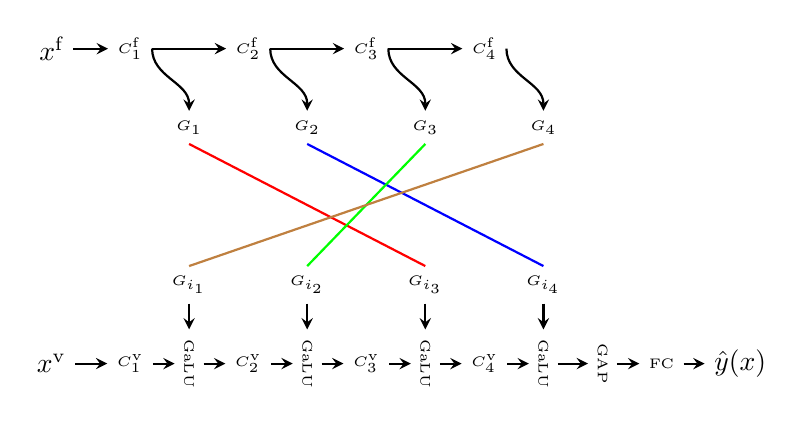
\begin{tikzpicture}
%\node []  (fntext)at (-4.625,-3.5) {CNN-GAP-DLGN};

%\node []  (output) at (7.5,1.5) {$\hat{y}(x)$};


\node [] (dgn1-f-c4) at (-3.5,1.5){\tiny{$C^{\text{f}}_4$}};
\node [] (dgn1-f-c3) at (-5,1.5){\tiny{$C^{\text{f}}_3$}};
\node [] (dgn1-f-c2) at (-6.5,1.5){\tiny{$C^{\text{f}}_2$}};
\node [] (dgn1-f-c1) at (-8,1.5){\tiny{$C^{\text{f}}_1$}};
\node [] (dgn1-input-f) at (-9,1.5){$x^{\text{f}}$};
\draw [-stealth,thick]   (dgn1-f-c3.east) -- (dgn1-f-c4.west);
\draw [-stealth,thick]   (dgn1-f-c2.east) -- (dgn1-f-c3.west);
\draw [-stealth,thick]   (dgn1-f-c1.east) -- (dgn1-f-c2.west);
\draw [-stealth,thick]   (dgn1-input-f.east) -- (dgn1-f-c1.west);



\node []  (dgn1-output) at (-0.25,-2.5) {$\hat{y}(x)$};

\node [] (dgn1-smax) at (-1.25,-2.5){\tiny{FC}};
\draw [-stealth,thick]   (dgn1-smax.east)--(dgn1-output.west);

\node [rotate=-90] (dgn1-gap) at (-2,-2.5){\tiny{GAP}};
\draw [-stealth,thick]   (dgn1-gap.north)--(dgn1-smax.west);


\node [rotate=-90] (dgn1-galu-4) at (-2.75,-2.5){\tiny{GaLU}};
\draw [-stealth,thick]   (dgn1-galu-4.north)--(dgn1-gap.south);

\node [] (dgn1-v-c4) at (-3.5,-2.5){\tiny{$C^{\text{v}}_4$}};
\draw [-stealth,thick]   (dgn1-v-c4.east) -- (dgn1-galu-4.south);


\node [rotate=-90] (dgn1-galu-3) at (-4.25,-2.5){\tiny{GaLU}};
\draw [-stealth,thick]   (dgn1-galu-3.north) -- (dgn1-v-c4.west);

\node [] (dgn1-v-c3) at (-5,-2.5){\tiny{$C^{\text{v}}_3$}};
\draw [-stealth,thick]   (dgn1-v-c3.east) -- (dgn1-galu-3.south);


\node [rotate=-90] (dgn1-galu-2) at (-5.75,-2.5){\tiny{GaLU}};
\draw [-stealth,thick]   (dgn1-galu-2.north) -- (dgn1-v-c3.west);

\node [] (dgn1-v-c2) at (-6.5,-2.5){\tiny{$C^{\text{v}}_2$}};
\draw [-stealth,thick]   (dgn1-v-c2.east) -- (dgn1-galu-2.south);


\node [rotate=-90] (dgn1-galu-1) at (-7.25,-2.5){\tiny{GaLU}};
\draw [-stealth,thick]   (dgn1-galu-1.north) -- (dgn1-v-c2.west);


\node [] (dgn1-v-c1) at (-8,-2.5){\tiny{$C^{\text{v}}_1$}};
\draw [-stealth,thick]   (dgn1-v-c1.east) -- (dgn1-galu-1.south);


\node [] (dgn1-v-input) at (-9,-2.5){$x^{\text{v}}$};

\draw [-stealth,thick]   (dgn1-v-input.east) -- (dgn1-v-c1.west);


\node[] (dgn1-gating-4-up) at (-2.75,0.5){\tiny{$G_{4}$}};
\draw [-stealth,thick]   (dgn1-f-c4.east) to[out=-90,in=90] (dgn1-gating-4-up.north);


\node[] (dgn1-gating-3-up) at (-4.25,0.5){\tiny{$G_{3}$}};
\draw [-stealth,thick]   (dgn1-f-c3.east) to[out=-90,in=90] (dgn1-gating-3-up.north);



\node[] (dgn1-gating-2-up) at (-5.75,0.5){\tiny{$G_{2}$}};
\draw [-stealth,thick]   (dgn1-f-c2.east) to[out=-90,in=90] (dgn1-gating-2-up.north);


\node[] (dgn1-gating-1-up) at (-7.25,0.5){\tiny{$G_{1}$}};
\draw [-stealth,thick]   (dgn1-f-c1.east) to[out=-90,in=90] (dgn1-gating-1-up.north);





\node[] (dgn1-gating-4) at (-2.75,-1.5){\tiny{$G_{i_4}$}};
\draw [-stealth,thick]   (dgn1-gating-4.south) -- (dgn1-galu-4.west);


\node[] (dgn1-gating-3) at (-4.25,-1.5){\tiny{$G_{i_3}$}};
\draw [-stealth,thick]   (dgn1-gating-3.south) -- (dgn1-galu-3.west);



\node[] (dgn1-gating-2) at (-5.75,-1.5){\tiny{$G_{i_2}$}};
\draw [-stealth,thick]   (dgn1-gating-2.south) -- (dgn1-galu-2.west);


\node[] (dgn1-gating-1) at (-7.25,-1.5){\tiny{$G_{i_1}$}};
\draw [-stealth,thick]   (dgn1-gating-1.south) -- (dgn1-galu-1.west);



\draw [-,thick,color=red]   (dgn1-gating-1-up.south) --(dgn1-gating-3.north);

\draw [-,thick,color=blue]   (dgn1-gating-2-up.south) --(dgn1-gating-4.north);

\draw [-,thick,color=green]   (dgn1-gating-3-up.south) --(dgn1-gating-2.north);

\draw [-,thick,color=brown]   (dgn1-gating-4-up.south) --(dgn1-gating-1.north);


%%%%%%%%%%%%%%%%%%%%%%%%%%%%%%%%%%%%%%%%%%%%%%%%%%%%%%%%%%%%%%%%%
	
\end{tikzpicture}


}
\end{minipage}
\begin{minipage}{0.48\columnwidth}
\centering
\resizebox{0.99\columnwidth}{!}{
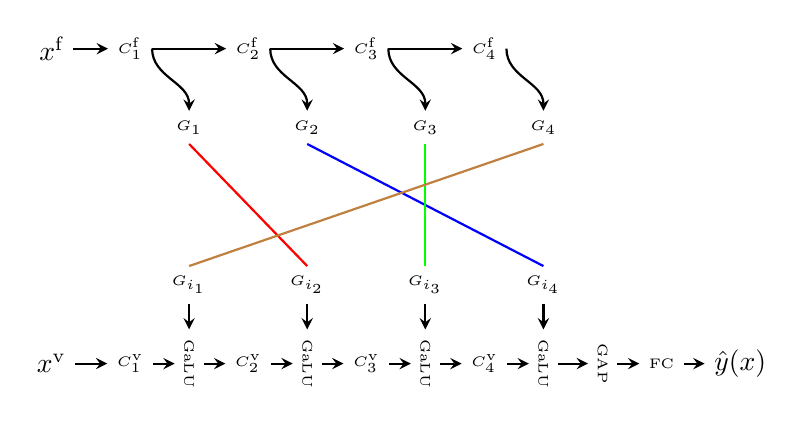
\begin{tikzpicture}
%\node []  (fntext)at (-4.625,-3.5) {CNN-GAP-DLGN};

%\node []  (output) at (7.5,1.5) {$\hat{y}(x)$};


\node [] (dgn1-f-c4) at (-3.5,1.5){\tiny{$C^{\text{f}}_4$}};
\node [] (dgn1-f-c3) at (-5,1.5){\tiny{$C^{\text{f}}_3$}};
\node [] (dgn1-f-c2) at (-6.5,1.5){\tiny{$C^{\text{f}}_2$}};
\node [] (dgn1-f-c1) at (-8,1.5){\tiny{$C^{\text{f}}_1$}};
\node [] (dgn1-input-f) at (-9,1.5){$x^{\text{f}}$};
\draw [-stealth,thick]   (dgn1-f-c3.east) -- (dgn1-f-c4.west);
\draw [-stealth,thick]   (dgn1-f-c2.east) -- (dgn1-f-c3.west);
\draw [-stealth,thick]   (dgn1-f-c1.east) -- (dgn1-f-c2.west);
\draw [-stealth,thick]   (dgn1-input-f.east) -- (dgn1-f-c1.west);



\node []  (dgn1-output) at (-0.25,-2.5) {$\hat{y}(x)$};

\node [] (dgn1-smax) at (-1.25,-2.5){\tiny{FC}};
\draw [-stealth,thick]   (dgn1-smax.east)--(dgn1-output.west);

\node [rotate=-90] (dgn1-gap) at (-2,-2.5){\tiny{GAP}};
\draw [-stealth,thick]   (dgn1-gap.north)--(dgn1-smax.west);


\node [rotate=-90] (dgn1-galu-4) at (-2.75,-2.5){\tiny{GaLU}};
\draw [-stealth,thick]   (dgn1-galu-4.north)--(dgn1-gap.south);

\node [] (dgn1-v-c4) at (-3.5,-2.5){\tiny{$C^{\text{v}}_4$}};
\draw [-stealth,thick]   (dgn1-v-c4.east) -- (dgn1-galu-4.south);


\node [rotate=-90] (dgn1-galu-3) at (-4.25,-2.5){\tiny{GaLU}};
\draw [-stealth,thick]   (dgn1-galu-3.north) -- (dgn1-v-c4.west);

\node [] (dgn1-v-c3) at (-5,-2.5){\tiny{$C^{\text{v}}_3$}};
\draw [-stealth,thick]   (dgn1-v-c3.east) -- (dgn1-galu-3.south);


\node [rotate=-90] (dgn1-galu-2) at (-5.75,-2.5){\tiny{GaLU}};
\draw [-stealth,thick]   (dgn1-galu-2.north) -- (dgn1-v-c3.west);

\node [] (dgn1-v-c2) at (-6.5,-2.5){\tiny{$C^{\text{v}}_2$}};
\draw [-stealth,thick]   (dgn1-v-c2.east) -- (dgn1-galu-2.south);


\node [rotate=-90] (dgn1-galu-1) at (-7.25,-2.5){\tiny{GaLU}};
\draw [-stealth,thick]   (dgn1-galu-1.north) -- (dgn1-v-c2.west);


\node [] (dgn1-v-c1) at (-8,-2.5){\tiny{$C^{\text{v}}_1$}};
\draw [-stealth,thick]   (dgn1-v-c1.east) -- (dgn1-galu-1.south);


\node [] (dgn1-v-input) at (-9,-2.5){$x^{\text{v}}$};

\draw [-stealth,thick]   (dgn1-v-input.east) -- (dgn1-v-c1.west);


\node[] (dgn1-gating-4-up) at (-2.75,0.5){\tiny{$G_{4}$}};
\draw [-stealth,thick]   (dgn1-f-c4.east) to[out=-90,in=90] (dgn1-gating-4-up.north);


\node[] (dgn1-gating-3-up) at (-4.25,0.5){\tiny{$G_{3}$}};
\draw [-stealth,thick]   (dgn1-f-c3.east) to[out=-90,in=90] (dgn1-gating-3-up.north);



\node[] (dgn1-gating-2-up) at (-5.75,0.5){\tiny{$G_{2}$}};
\draw [-stealth,thick]   (dgn1-f-c2.east) to[out=-90,in=90] (dgn1-gating-2-up.north);


\node[] (dgn1-gating-1-up) at (-7.25,0.5){\tiny{$G_{1}$}};
\draw [-stealth,thick]   (dgn1-f-c1.east) to[out=-90,in=90] (dgn1-gating-1-up.north);





\node[] (dgn1-gating-4) at (-2.75,-1.5){\tiny{$G_{i_4}$}};
\draw [-stealth,thick]   (dgn1-gating-4.south) -- (dgn1-galu-4.west);


\node[] (dgn1-gating-3) at (-4.25,-1.5){\tiny{$G_{i_3}$}};
\draw [-stealth,thick]   (dgn1-gating-3.south) -- (dgn1-galu-3.west);



\node[] (dgn1-gating-2) at (-5.75,-1.5){\tiny{$G_{i_2}$}};
\draw [-stealth,thick]   (dgn1-gating-2.south) -- (dgn1-galu-2.west);


\node[] (dgn1-gating-1) at (-7.25,-1.5){\tiny{$G_{i_1}$}};
\draw [-stealth,thick]   (dgn1-gating-1.south) -- (dgn1-galu-1.west);



\draw [-,thick,color=red]   (dgn1-gating-1-up.south) --(dgn1-gating-2.north);

\draw [-,thick,color=blue]   (dgn1-gating-2-up.south) --(dgn1-gating-4.north);

\draw [-,thick,color=green]   (dgn1-gating-3-up.south) --(dgn1-gating-3.north);

\draw [-,thick,color=brown]   (dgn1-gating-4-up.south) --(dgn1-gating-1.north);


%%%%%%%%%%%%%%%%%%%%%%%%%%%%%%%%%%%%%%%%%%%%%%%%%%%%%%%%%%%%%%%%%
	
\end{tikzpicture}


}
\end{minipage}

\begin{minipage}{0.48\columnwidth}
\centering
\resizebox{0.99\columnwidth}{!}{
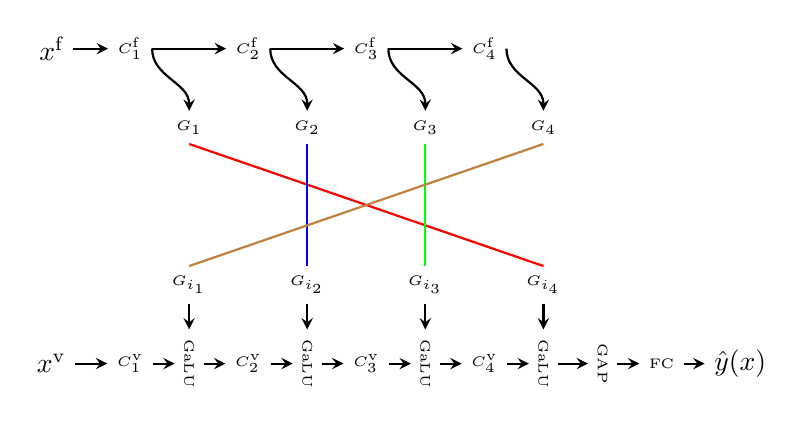
\begin{tikzpicture}
%\node []  (fntext)at (-4.625,-3.5) {CNN-GAP-DLGN};

%\node []  (output) at (7.5,1.5) {$\hat{y}(x)$};


\node [] (dgn1-f-c4) at (-3.5,1.5){\tiny{$C^{\text{f}}_4$}};
\node [] (dgn1-f-c3) at (-5,1.5){\tiny{$C^{\text{f}}_3$}};
\node [] (dgn1-f-c2) at (-6.5,1.5){\tiny{$C^{\text{f}}_2$}};
\node [] (dgn1-f-c1) at (-8,1.5){\tiny{$C^{\text{f}}_1$}};
\node [] (dgn1-input-f) at (-9,1.5){$x^{\text{f}}$};
\draw [-stealth,thick]   (dgn1-f-c3.east) -- (dgn1-f-c4.west);
\draw [-stealth,thick]   (dgn1-f-c2.east) -- (dgn1-f-c3.west);
\draw [-stealth,thick]   (dgn1-f-c1.east) -- (dgn1-f-c2.west);
\draw [-stealth,thick]   (dgn1-input-f.east) -- (dgn1-f-c1.west);



\node []  (dgn1-output) at (-0.25,-2.5) {$\hat{y}(x)$};

\node [] (dgn1-smax) at (-1.25,-2.5){\tiny{FC}};
\draw [-stealth,thick]   (dgn1-smax.east)--(dgn1-output.west);

\node [rotate=-90] (dgn1-gap) at (-2,-2.5){\tiny{GAP}};
\draw [-stealth,thick]   (dgn1-gap.north)--(dgn1-smax.west);


\node [rotate=-90] (dgn1-galu-4) at (-2.75,-2.5){\tiny{GaLU}};
\draw [-stealth,thick]   (dgn1-galu-4.north)--(dgn1-gap.south);

\node [] (dgn1-v-c4) at (-3.5,-2.5){\tiny{$C^{\text{v}}_4$}};
\draw [-stealth,thick]   (dgn1-v-c4.east) -- (dgn1-galu-4.south);


\node [rotate=-90] (dgn1-galu-3) at (-4.25,-2.5){\tiny{GaLU}};
\draw [-stealth,thick]   (dgn1-galu-3.north) -- (dgn1-v-c4.west);

\node [] (dgn1-v-c3) at (-5,-2.5){\tiny{$C^{\text{v}}_3$}};
\draw [-stealth,thick]   (dgn1-v-c3.east) -- (dgn1-galu-3.south);


\node [rotate=-90] (dgn1-galu-2) at (-5.75,-2.5){\tiny{GaLU}};
\draw [-stealth,thick]   (dgn1-galu-2.north) -- (dgn1-v-c3.west);

\node [] (dgn1-v-c2) at (-6.5,-2.5){\tiny{$C^{\text{v}}_2$}};
\draw [-stealth,thick]   (dgn1-v-c2.east) -- (dgn1-galu-2.south);


\node [rotate=-90] (dgn1-galu-1) at (-7.25,-2.5){\tiny{GaLU}};
\draw [-stealth,thick]   (dgn1-galu-1.north) -- (dgn1-v-c2.west);


\node [] (dgn1-v-c1) at (-8,-2.5){\tiny{$C^{\text{v}}_1$}};
\draw [-stealth,thick]   (dgn1-v-c1.east) -- (dgn1-galu-1.south);


\node [] (dgn1-v-input) at (-9,-2.5){$x^{\text{v}}$};

\draw [-stealth,thick]   (dgn1-v-input.east) -- (dgn1-v-c1.west);


\node[] (dgn1-gating-4-up) at (-2.75,0.5){\tiny{$G_{4}$}};
\draw [-stealth,thick]   (dgn1-f-c4.east) to[out=-90,in=90] (dgn1-gating-4-up.north);


\node[] (dgn1-gating-3-up) at (-4.25,0.5){\tiny{$G_{3}$}};
\draw [-stealth,thick]   (dgn1-f-c3.east) to[out=-90,in=90] (dgn1-gating-3-up.north);



\node[] (dgn1-gating-2-up) at (-5.75,0.5){\tiny{$G_{2}$}};
\draw [-stealth,thick]   (dgn1-f-c2.east) to[out=-90,in=90] (dgn1-gating-2-up.north);


\node[] (dgn1-gating-1-up) at (-7.25,0.5){\tiny{$G_{1}$}};
\draw [-stealth,thick]   (dgn1-f-c1.east) to[out=-90,in=90] (dgn1-gating-1-up.north);





\node[] (dgn1-gating-4) at (-2.75,-1.5){\tiny{$G_{i_4}$}};
\draw [-stealth,thick]   (dgn1-gating-4.south) -- (dgn1-galu-4.west);


\node[] (dgn1-gating-3) at (-4.25,-1.5){\tiny{$G_{i_3}$}};
\draw [-stealth,thick]   (dgn1-gating-3.south) -- (dgn1-galu-3.west);



\node[] (dgn1-gating-2) at (-5.75,-1.5){\tiny{$G_{i_2}$}};
\draw [-stealth,thick]   (dgn1-gating-2.south) -- (dgn1-galu-2.west);


\node[] (dgn1-gating-1) at (-7.25,-1.5){\tiny{$G_{i_1}$}};
\draw [-stealth,thick]   (dgn1-gating-1.south) -- (dgn1-galu-1.west);



\draw [-,thick,color=red]   (dgn1-gating-1-up.south) --(dgn1-gating-4.north);

\draw [-,thick,color=blue]   (dgn1-gating-2-up.south) --(dgn1-gating-2.north);

\draw [-,thick,color=green]   (dgn1-gating-3-up.south) --(dgn1-gating-3.north);

\draw [-,thick,color=brown]   (dgn1-gating-4-up.south) --(dgn1-gating-1.north);


%%%%%%%%%%%%%%%%%%%%%%%%%%%%%%%%%%%%%%%%%%%%%%%%%%%%%%%%%%%%%%%%%
	
\end{tikzpicture}


}
\end{minipage}
\begin{minipage}{0.48\columnwidth}
\centering
\resizebox{0.99\columnwidth}{!}{
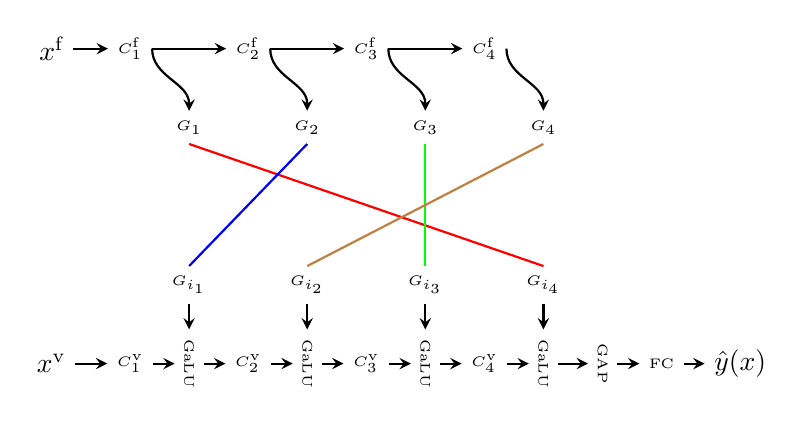
\begin{tikzpicture}
%\node []  (fntext)at (-4.625,-3.5) {CNN-GAP-DLGN};

%\node []  (output) at (7.5,1.5) {$\hat{y}(x)$};


\node [] (dgn1-f-c4) at (-3.5,1.5){\tiny{$C^{\text{f}}_4$}};
\node [] (dgn1-f-c3) at (-5,1.5){\tiny{$C^{\text{f}}_3$}};
\node [] (dgn1-f-c2) at (-6.5,1.5){\tiny{$C^{\text{f}}_2$}};
\node [] (dgn1-f-c1) at (-8,1.5){\tiny{$C^{\text{f}}_1$}};
\node [] (dgn1-input-f) at (-9,1.5){$x^{\text{f}}$};
\draw [-stealth,thick]   (dgn1-f-c3.east) -- (dgn1-f-c4.west);
\draw [-stealth,thick]   (dgn1-f-c2.east) -- (dgn1-f-c3.west);
\draw [-stealth,thick]   (dgn1-f-c1.east) -- (dgn1-f-c2.west);
\draw [-stealth,thick]   (dgn1-input-f.east) -- (dgn1-f-c1.west);



\node []  (dgn1-output) at (-0.25,-2.5) {$\hat{y}(x)$};

\node [] (dgn1-smax) at (-1.25,-2.5){\tiny{FC}};
\draw [-stealth,thick]   (dgn1-smax.east)--(dgn1-output.west);

\node [rotate=-90] (dgn1-gap) at (-2,-2.5){\tiny{GAP}};
\draw [-stealth,thick]   (dgn1-gap.north)--(dgn1-smax.west);


\node [rotate=-90] (dgn1-galu-4) at (-2.75,-2.5){\tiny{GaLU}};
\draw [-stealth,thick]   (dgn1-galu-4.north)--(dgn1-gap.south);

\node [] (dgn1-v-c4) at (-3.5,-2.5){\tiny{$C^{\text{v}}_4$}};
\draw [-stealth,thick]   (dgn1-v-c4.east) -- (dgn1-galu-4.south);


\node [rotate=-90] (dgn1-galu-3) at (-4.25,-2.5){\tiny{GaLU}};
\draw [-stealth,thick]   (dgn1-galu-3.north) -- (dgn1-v-c4.west);

\node [] (dgn1-v-c3) at (-5,-2.5){\tiny{$C^{\text{v}}_3$}};
\draw [-stealth,thick]   (dgn1-v-c3.east) -- (dgn1-galu-3.south);


\node [rotate=-90] (dgn1-galu-2) at (-5.75,-2.5){\tiny{GaLU}};
\draw [-stealth,thick]   (dgn1-galu-2.north) -- (dgn1-v-c3.west);

\node [] (dgn1-v-c2) at (-6.5,-2.5){\tiny{$C^{\text{v}}_2$}};
\draw [-stealth,thick]   (dgn1-v-c2.east) -- (dgn1-galu-2.south);


\node [rotate=-90] (dgn1-galu-1) at (-7.25,-2.5){\tiny{GaLU}};
\draw [-stealth,thick]   (dgn1-galu-1.north) -- (dgn1-v-c2.west);


\node [] (dgn1-v-c1) at (-8,-2.5){\tiny{$C^{\text{v}}_1$}};
\draw [-stealth,thick]   (dgn1-v-c1.east) -- (dgn1-galu-1.south);


\node [] (dgn1-v-input) at (-9,-2.5){$x^{\text{v}}$};

\draw [-stealth,thick]   (dgn1-v-input.east) -- (dgn1-v-c1.west);


\node[] (dgn1-gating-4-up) at (-2.75,0.5){\tiny{$G_{4}$}};
\draw [-stealth,thick]   (dgn1-f-c4.east) to[out=-90,in=90] (dgn1-gating-4-up.north);


\node[] (dgn1-gating-3-up) at (-4.25,0.5){\tiny{$G_{3}$}};
\draw [-stealth,thick]   (dgn1-f-c3.east) to[out=-90,in=90] (dgn1-gating-3-up.north);



\node[] (dgn1-gating-2-up) at (-5.75,0.5){\tiny{$G_{2}$}};
\draw [-stealth,thick]   (dgn1-f-c2.east) to[out=-90,in=90] (dgn1-gating-2-up.north);


\node[] (dgn1-gating-1-up) at (-7.25,0.5){\tiny{$G_{1}$}};
\draw [-stealth,thick]   (dgn1-f-c1.east) to[out=-90,in=90] (dgn1-gating-1-up.north);





\node[] (dgn1-gating-4) at (-2.75,-1.5){\tiny{$G_{i_4}$}};
\draw [-stealth,thick]   (dgn1-gating-4.south) -- (dgn1-galu-4.west);


\node[] (dgn1-gating-3) at (-4.25,-1.5){\tiny{$G_{i_3}$}};
\draw [-stealth,thick]   (dgn1-gating-3.south) -- (dgn1-galu-3.west);



\node[] (dgn1-gating-2) at (-5.75,-1.5){\tiny{$G_{i_2}$}};
\draw [-stealth,thick]   (dgn1-gating-2.south) -- (dgn1-galu-2.west);


\node[] (dgn1-gating-1) at (-7.25,-1.5){\tiny{$G_{i_1}$}};
\draw [-stealth,thick]   (dgn1-gating-1.south) -- (dgn1-galu-1.west);



\draw [-,thick,color=red]   (dgn1-gating-1-up.south) --(dgn1-gating-4.north);

\draw [-,thick,color=blue]   (dgn1-gating-2-up.south) --(dgn1-gating-1.north);

\draw [-,thick,color=green]   (dgn1-gating-3-up.south) --(dgn1-gating-3.north);

\draw [-,thick,color=brown]   (dgn1-gating-4-up.south) --(dgn1-gating-2.north);


%%%%%%%%%%%%%%%%%%%%%%%%%%%%%%%%%%%%%%%%%%%%%%%%%%%%%%%%%%%%%%%%%
	
\end{tikzpicture}


}
\end{minipage}

\caption{Shows the permutations $1-12$ C4GAP-DLGN in Table I of \Cref{fig:c4gap}. The top left is the identity permutation and is the vanilla model.}
\label{fig:perm1}
\end{figure}

\begin{figure}
\centering
\begin{minipage}{0.48\columnwidth}
\centering
\resizebox{0.99\columnwidth}{!}{
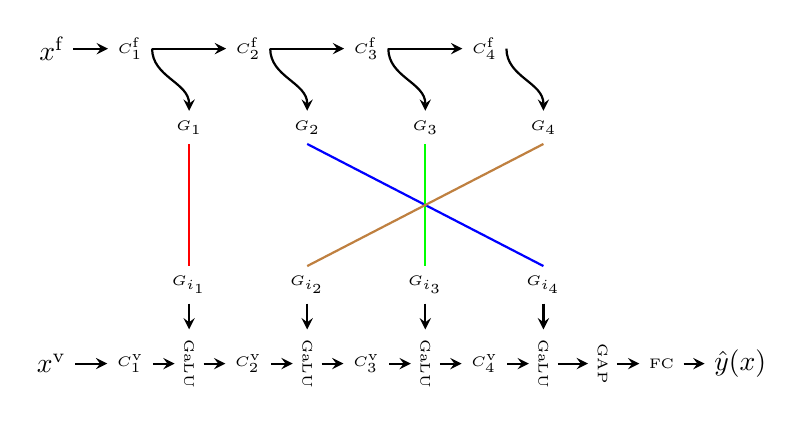
\begin{tikzpicture}
%\node []  (fntext)at (-4.625,-3.5) {CNN-GAP-DLGN};

%\node []  (output) at (7.5,1.5) {$\hat{y}(x)$};


\node [] (dgn1-f-c4) at (-3.5,1.5){\tiny{$C^{\text{f}}_4$}};
\node [] (dgn1-f-c3) at (-5,1.5){\tiny{$C^{\text{f}}_3$}};
\node [] (dgn1-f-c2) at (-6.5,1.5){\tiny{$C^{\text{f}}_2$}};
\node [] (dgn1-f-c1) at (-8,1.5){\tiny{$C^{\text{f}}_1$}};
\node [] (dgn1-input-f) at (-9,1.5){$x^{\text{f}}$};
\draw [-stealth,thick]   (dgn1-f-c3.east) -- (dgn1-f-c4.west);
\draw [-stealth,thick]   (dgn1-f-c2.east) -- (dgn1-f-c3.west);
\draw [-stealth,thick]   (dgn1-f-c1.east) -- (dgn1-f-c2.west);
\draw [-stealth,thick]   (dgn1-input-f.east) -- (dgn1-f-c1.west);



\node []  (dgn1-output) at (-0.25,-2.5) {$\hat{y}(x)$};

\node [] (dgn1-smax) at (-1.25,-2.5){\tiny{FC}};
\draw [-stealth,thick]   (dgn1-smax.east)--(dgn1-output.west);

\node [rotate=-90] (dgn1-gap) at (-2,-2.5){\tiny{GAP}};
\draw [-stealth,thick]   (dgn1-gap.north)--(dgn1-smax.west);


\node [rotate=-90] (dgn1-galu-4) at (-2.75,-2.5){\tiny{GaLU}};
\draw [-stealth,thick]   (dgn1-galu-4.north)--(dgn1-gap.south);

\node [] (dgn1-v-c4) at (-3.5,-2.5){\tiny{$C^{\text{v}}_4$}};
\draw [-stealth,thick]   (dgn1-v-c4.east) -- (dgn1-galu-4.south);


\node [rotate=-90] (dgn1-galu-3) at (-4.25,-2.5){\tiny{GaLU}};
\draw [-stealth,thick]   (dgn1-galu-3.north) -- (dgn1-v-c4.west);

\node [] (dgn1-v-c3) at (-5,-2.5){\tiny{$C^{\text{v}}_3$}};
\draw [-stealth,thick]   (dgn1-v-c3.east) -- (dgn1-galu-3.south);


\node [rotate=-90] (dgn1-galu-2) at (-5.75,-2.5){\tiny{GaLU}};
\draw [-stealth,thick]   (dgn1-galu-2.north) -- (dgn1-v-c3.west);

\node [] (dgn1-v-c2) at (-6.5,-2.5){\tiny{$C^{\text{v}}_2$}};
\draw [-stealth,thick]   (dgn1-v-c2.east) -- (dgn1-galu-2.south);


\node [rotate=-90] (dgn1-galu-1) at (-7.25,-2.5){\tiny{GaLU}};
\draw [-stealth,thick]   (dgn1-galu-1.north) -- (dgn1-v-c2.west);


\node [] (dgn1-v-c1) at (-8,-2.5){\tiny{$C^{\text{v}}_1$}};
\draw [-stealth,thick]   (dgn1-v-c1.east) -- (dgn1-galu-1.south);


\node [] (dgn1-v-input) at (-9,-2.5){$x^{\text{v}}$};

\draw [-stealth,thick]   (dgn1-v-input.east) -- (dgn1-v-c1.west);


\node[] (dgn1-gating-4-up) at (-2.75,0.5){\tiny{$G_{4}$}};
\draw [-stealth,thick]   (dgn1-f-c4.east) to[out=-90,in=90] (dgn1-gating-4-up.north);


\node[] (dgn1-gating-3-up) at (-4.25,0.5){\tiny{$G_{3}$}};
\draw [-stealth,thick]   (dgn1-f-c3.east) to[out=-90,in=90] (dgn1-gating-3-up.north);



\node[] (dgn1-gating-2-up) at (-5.75,0.5){\tiny{$G_{2}$}};
\draw [-stealth,thick]   (dgn1-f-c2.east) to[out=-90,in=90] (dgn1-gating-2-up.north);


\node[] (dgn1-gating-1-up) at (-7.25,0.5){\tiny{$G_{1}$}};
\draw [-stealth,thick]   (dgn1-f-c1.east) to[out=-90,in=90] (dgn1-gating-1-up.north);





\node[] (dgn1-gating-4) at (-2.75,-1.5){\tiny{$G_{i_4}$}};
\draw [-stealth,thick]   (dgn1-gating-4.south) -- (dgn1-galu-4.west);


\node[] (dgn1-gating-3) at (-4.25,-1.5){\tiny{$G_{i_3}$}};
\draw [-stealth,thick]   (dgn1-gating-3.south) -- (dgn1-galu-3.west);



\node[] (dgn1-gating-2) at (-5.75,-1.5){\tiny{$G_{i_2}$}};
\draw [-stealth,thick]   (dgn1-gating-2.south) -- (dgn1-galu-2.west);


\node[] (dgn1-gating-1) at (-7.25,-1.5){\tiny{$G_{i_1}$}};
\draw [-stealth,thick]   (dgn1-gating-1.south) -- (dgn1-galu-1.west);



\draw [-,thick,color=red]   (dgn1-gating-1-up.south) --(dgn1-gating-1.north);

\draw [-,thick,color=blue]   (dgn1-gating-2-up.south) --(dgn1-gating-4.north);

\draw [-,thick,color=green]   (dgn1-gating-3-up.south) --(dgn1-gating-3.north);

\draw [-,thick,color=brown]   (dgn1-gating-4-up.south) --(dgn1-gating-2.north);


%%%%%%%%%%%%%%%%%%%%%%%%%%%%%%%%%%%%%%%%%%%%%%%%%%%%%%%%%%%%%%%%%
	
\end{tikzpicture}


}
\end{minipage}
\begin{minipage}{0.48\columnwidth}
\centering
\resizebox{0.99\columnwidth}{!}{
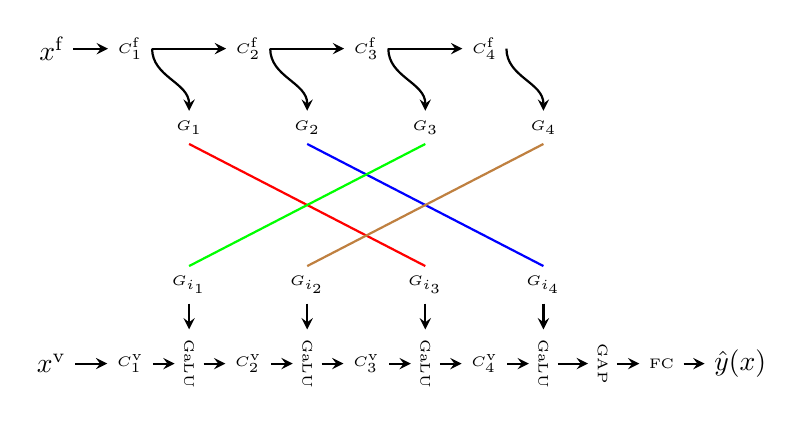
\begin{tikzpicture}
%\node []  (fntext)at (-4.625,-3.5) {CNN-GAP-DLGN};

%\node []  (output) at (7.5,1.5) {$\hat{y}(x)$};


\node [] (dgn1-f-c4) at (-3.5,1.5){\tiny{$C^{\text{f}}_4$}};
\node [] (dgn1-f-c3) at (-5,1.5){\tiny{$C^{\text{f}}_3$}};
\node [] (dgn1-f-c2) at (-6.5,1.5){\tiny{$C^{\text{f}}_2$}};
\node [] (dgn1-f-c1) at (-8,1.5){\tiny{$C^{\text{f}}_1$}};
\node [] (dgn1-input-f) at (-9,1.5){$x^{\text{f}}$};
\draw [-stealth,thick]   (dgn1-f-c3.east) -- (dgn1-f-c4.west);
\draw [-stealth,thick]   (dgn1-f-c2.east) -- (dgn1-f-c3.west);
\draw [-stealth,thick]   (dgn1-f-c1.east) -- (dgn1-f-c2.west);
\draw [-stealth,thick]   (dgn1-input-f.east) -- (dgn1-f-c1.west);



\node []  (dgn1-output) at (-0.25,-2.5) {$\hat{y}(x)$};

\node [] (dgn1-smax) at (-1.25,-2.5){\tiny{FC}};
\draw [-stealth,thick]   (dgn1-smax.east)--(dgn1-output.west);

\node [rotate=-90] (dgn1-gap) at (-2,-2.5){\tiny{GAP}};
\draw [-stealth,thick]   (dgn1-gap.north)--(dgn1-smax.west);


\node [rotate=-90] (dgn1-galu-4) at (-2.75,-2.5){\tiny{GaLU}};
\draw [-stealth,thick]   (dgn1-galu-4.north)--(dgn1-gap.south);

\node [] (dgn1-v-c4) at (-3.5,-2.5){\tiny{$C^{\text{v}}_4$}};
\draw [-stealth,thick]   (dgn1-v-c4.east) -- (dgn1-galu-4.south);


\node [rotate=-90] (dgn1-galu-3) at (-4.25,-2.5){\tiny{GaLU}};
\draw [-stealth,thick]   (dgn1-galu-3.north) -- (dgn1-v-c4.west);

\node [] (dgn1-v-c3) at (-5,-2.5){\tiny{$C^{\text{v}}_3$}};
\draw [-stealth,thick]   (dgn1-v-c3.east) -- (dgn1-galu-3.south);


\node [rotate=-90] (dgn1-galu-2) at (-5.75,-2.5){\tiny{GaLU}};
\draw [-stealth,thick]   (dgn1-galu-2.north) -- (dgn1-v-c3.west);

\node [] (dgn1-v-c2) at (-6.5,-2.5){\tiny{$C^{\text{v}}_2$}};
\draw [-stealth,thick]   (dgn1-v-c2.east) -- (dgn1-galu-2.south);


\node [rotate=-90] (dgn1-galu-1) at (-7.25,-2.5){\tiny{GaLU}};
\draw [-stealth,thick]   (dgn1-galu-1.north) -- (dgn1-v-c2.west);


\node [] (dgn1-v-c1) at (-8,-2.5){\tiny{$C^{\text{v}}_1$}};
\draw [-stealth,thick]   (dgn1-v-c1.east) -- (dgn1-galu-1.south);


\node [] (dgn1-v-input) at (-9,-2.5){$x^{\text{v}}$};

\draw [-stealth,thick]   (dgn1-v-input.east) -- (dgn1-v-c1.west);


\node[] (dgn1-gating-4-up) at (-2.75,0.5){\tiny{$G_{4}$}};
\draw [-stealth,thick]   (dgn1-f-c4.east) to[out=-90,in=90] (dgn1-gating-4-up.north);


\node[] (dgn1-gating-3-up) at (-4.25,0.5){\tiny{$G_{3}$}};
\draw [-stealth,thick]   (dgn1-f-c3.east) to[out=-90,in=90] (dgn1-gating-3-up.north);



\node[] (dgn1-gating-2-up) at (-5.75,0.5){\tiny{$G_{2}$}};
\draw [-stealth,thick]   (dgn1-f-c2.east) to[out=-90,in=90] (dgn1-gating-2-up.north);


\node[] (dgn1-gating-1-up) at (-7.25,0.5){\tiny{$G_{1}$}};
\draw [-stealth,thick]   (dgn1-f-c1.east) to[out=-90,in=90] (dgn1-gating-1-up.north);





\node[] (dgn1-gating-4) at (-2.75,-1.5){\tiny{$G_{i_4}$}};
\draw [-stealth,thick]   (dgn1-gating-4.south) -- (dgn1-galu-4.west);


\node[] (dgn1-gating-3) at (-4.25,-1.5){\tiny{$G_{i_3}$}};
\draw [-stealth,thick]   (dgn1-gating-3.south) -- (dgn1-galu-3.west);



\node[] (dgn1-gating-2) at (-5.75,-1.5){\tiny{$G_{i_2}$}};
\draw [-stealth,thick]   (dgn1-gating-2.south) -- (dgn1-galu-2.west);


\node[] (dgn1-gating-1) at (-7.25,-1.5){\tiny{$G_{i_1}$}};
\draw [-stealth,thick]   (dgn1-gating-1.south) -- (dgn1-galu-1.west);



\draw [-,thick,color=red]   (dgn1-gating-1-up.south) --(dgn1-gating-3.north);

\draw [-,thick,color=blue]   (dgn1-gating-2-up.south) --(dgn1-gating-4.north);

\draw [-,thick,color=green]   (dgn1-gating-3-up.south) --(dgn1-gating-1.north);

\draw [-,thick,color=brown]   (dgn1-gating-4-up.south) --(dgn1-gating-2.north);


%%%%%%%%%%%%%%%%%%%%%%%%%%%%%%%%%%%%%%%%%%%%%%%%%%%%%%%%%%%%%%%%%
	
\end{tikzpicture}


}
\end{minipage}

\begin{minipage}{0.48\columnwidth}
\centering
\resizebox{0.99\columnwidth}{!}{
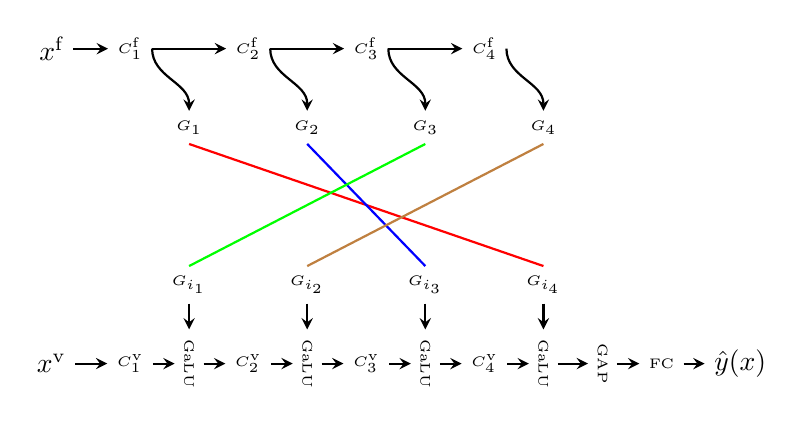
\begin{tikzpicture}
%\node []  (fntext)at (-4.625,-3.5) {CNN-GAP-DLGN};

%\node []  (output) at (7.5,1.5) {$\hat{y}(x)$};


\node [] (dgn1-f-c4) at (-3.5,1.5){\tiny{$C^{\text{f}}_4$}};
\node [] (dgn1-f-c3) at (-5,1.5){\tiny{$C^{\text{f}}_3$}};
\node [] (dgn1-f-c2) at (-6.5,1.5){\tiny{$C^{\text{f}}_2$}};
\node [] (dgn1-f-c1) at (-8,1.5){\tiny{$C^{\text{f}}_1$}};
\node [] (dgn1-input-f) at (-9,1.5){$x^{\text{f}}$};
\draw [-stealth,thick]   (dgn1-f-c3.east) -- (dgn1-f-c4.west);
\draw [-stealth,thick]   (dgn1-f-c2.east) -- (dgn1-f-c3.west);
\draw [-stealth,thick]   (dgn1-f-c1.east) -- (dgn1-f-c2.west);
\draw [-stealth,thick]   (dgn1-input-f.east) -- (dgn1-f-c1.west);



\node []  (dgn1-output) at (-0.25,-2.5) {$\hat{y}(x)$};

\node [] (dgn1-smax) at (-1.25,-2.5){\tiny{FC}};
\draw [-stealth,thick]   (dgn1-smax.east)--(dgn1-output.west);

\node [rotate=-90] (dgn1-gap) at (-2,-2.5){\tiny{GAP}};
\draw [-stealth,thick]   (dgn1-gap.north)--(dgn1-smax.west);


\node [rotate=-90] (dgn1-galu-4) at (-2.75,-2.5){\tiny{GaLU}};
\draw [-stealth,thick]   (dgn1-galu-4.north)--(dgn1-gap.south);

\node [] (dgn1-v-c4) at (-3.5,-2.5){\tiny{$C^{\text{v}}_4$}};
\draw [-stealth,thick]   (dgn1-v-c4.east) -- (dgn1-galu-4.south);


\node [rotate=-90] (dgn1-galu-3) at (-4.25,-2.5){\tiny{GaLU}};
\draw [-stealth,thick]   (dgn1-galu-3.north) -- (dgn1-v-c4.west);

\node [] (dgn1-v-c3) at (-5,-2.5){\tiny{$C^{\text{v}}_3$}};
\draw [-stealth,thick]   (dgn1-v-c3.east) -- (dgn1-galu-3.south);


\node [rotate=-90] (dgn1-galu-2) at (-5.75,-2.5){\tiny{GaLU}};
\draw [-stealth,thick]   (dgn1-galu-2.north) -- (dgn1-v-c3.west);

\node [] (dgn1-v-c2) at (-6.5,-2.5){\tiny{$C^{\text{v}}_2$}};
\draw [-stealth,thick]   (dgn1-v-c2.east) -- (dgn1-galu-2.south);


\node [rotate=-90] (dgn1-galu-1) at (-7.25,-2.5){\tiny{GaLU}};
\draw [-stealth,thick]   (dgn1-galu-1.north) -- (dgn1-v-c2.west);


\node [] (dgn1-v-c1) at (-8,-2.5){\tiny{$C^{\text{v}}_1$}};
\draw [-stealth,thick]   (dgn1-v-c1.east) -- (dgn1-galu-1.south);


\node [] (dgn1-v-input) at (-9,-2.5){$x^{\text{v}}$};

\draw [-stealth,thick]   (dgn1-v-input.east) -- (dgn1-v-c1.west);


\node[] (dgn1-gating-4-up) at (-2.75,0.5){\tiny{$G_{4}$}};
\draw [-stealth,thick]   (dgn1-f-c4.east) to[out=-90,in=90] (dgn1-gating-4-up.north);


\node[] (dgn1-gating-3-up) at (-4.25,0.5){\tiny{$G_{3}$}};
\draw [-stealth,thick]   (dgn1-f-c3.east) to[out=-90,in=90] (dgn1-gating-3-up.north);



\node[] (dgn1-gating-2-up) at (-5.75,0.5){\tiny{$G_{2}$}};
\draw [-stealth,thick]   (dgn1-f-c2.east) to[out=-90,in=90] (dgn1-gating-2-up.north);


\node[] (dgn1-gating-1-up) at (-7.25,0.5){\tiny{$G_{1}$}};
\draw [-stealth,thick]   (dgn1-f-c1.east) to[out=-90,in=90] (dgn1-gating-1-up.north);





\node[] (dgn1-gating-4) at (-2.75,-1.5){\tiny{$G_{i_4}$}};
\draw [-stealth,thick]   (dgn1-gating-4.south) -- (dgn1-galu-4.west);


\node[] (dgn1-gating-3) at (-4.25,-1.5){\tiny{$G_{i_3}$}};
\draw [-stealth,thick]   (dgn1-gating-3.south) -- (dgn1-galu-3.west);



\node[] (dgn1-gating-2) at (-5.75,-1.5){\tiny{$G_{i_2}$}};
\draw [-stealth,thick]   (dgn1-gating-2.south) -- (dgn1-galu-2.west);


\node[] (dgn1-gating-1) at (-7.25,-1.5){\tiny{$G_{i_1}$}};
\draw [-stealth,thick]   (dgn1-gating-1.south) -- (dgn1-galu-1.west);



\draw [-,thick,color=red]   (dgn1-gating-1-up.south) --(dgn1-gating-4.north);

\draw [-,thick,color=blue]   (dgn1-gating-2-up.south) --(dgn1-gating-3.north);

\draw [-,thick,color=green]   (dgn1-gating-3-up.south) --(dgn1-gating-1.north);

\draw [-,thick,color=brown]   (dgn1-gating-4-up.south) --(dgn1-gating-2.north);


%%%%%%%%%%%%%%%%%%%%%%%%%%%%%%%%%%%%%%%%%%%%%%%%%%%%%%%%%%%%%%%%%
	
\end{tikzpicture}


}
\end{minipage}
\begin{minipage}{0.48\columnwidth}
\centering
\resizebox{0.99\columnwidth}{!}{
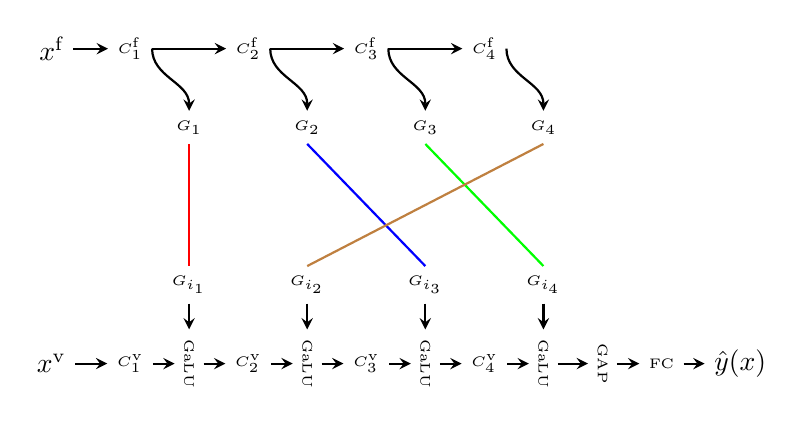
\begin{tikzpicture}
%\node []  (fntext)at (-4.625,-3.5) {CNN-GAP-DLGN};

%\node []  (output) at (7.5,1.5) {$\hat{y}(x)$};


\node [] (dgn1-f-c4) at (-3.5,1.5){\tiny{$C^{\text{f}}_4$}};
\node [] (dgn1-f-c3) at (-5,1.5){\tiny{$C^{\text{f}}_3$}};
\node [] (dgn1-f-c2) at (-6.5,1.5){\tiny{$C^{\text{f}}_2$}};
\node [] (dgn1-f-c1) at (-8,1.5){\tiny{$C^{\text{f}}_1$}};
\node [] (dgn1-input-f) at (-9,1.5){$x^{\text{f}}$};
\draw [-stealth,thick]   (dgn1-f-c3.east) -- (dgn1-f-c4.west);
\draw [-stealth,thick]   (dgn1-f-c2.east) -- (dgn1-f-c3.west);
\draw [-stealth,thick]   (dgn1-f-c1.east) -- (dgn1-f-c2.west);
\draw [-stealth,thick]   (dgn1-input-f.east) -- (dgn1-f-c1.west);



\node []  (dgn1-output) at (-0.25,-2.5) {$\hat{y}(x)$};

\node [] (dgn1-smax) at (-1.25,-2.5){\tiny{FC}};
\draw [-stealth,thick]   (dgn1-smax.east)--(dgn1-output.west);

\node [rotate=-90] (dgn1-gap) at (-2,-2.5){\tiny{GAP}};
\draw [-stealth,thick]   (dgn1-gap.north)--(dgn1-smax.west);


\node [rotate=-90] (dgn1-galu-4) at (-2.75,-2.5){\tiny{GaLU}};
\draw [-stealth,thick]   (dgn1-galu-4.north)--(dgn1-gap.south);

\node [] (dgn1-v-c4) at (-3.5,-2.5){\tiny{$C^{\text{v}}_4$}};
\draw [-stealth,thick]   (dgn1-v-c4.east) -- (dgn1-galu-4.south);


\node [rotate=-90] (dgn1-galu-3) at (-4.25,-2.5){\tiny{GaLU}};
\draw [-stealth,thick]   (dgn1-galu-3.north) -- (dgn1-v-c4.west);

\node [] (dgn1-v-c3) at (-5,-2.5){\tiny{$C^{\text{v}}_3$}};
\draw [-stealth,thick]   (dgn1-v-c3.east) -- (dgn1-galu-3.south);


\node [rotate=-90] (dgn1-galu-2) at (-5.75,-2.5){\tiny{GaLU}};
\draw [-stealth,thick]   (dgn1-galu-2.north) -- (dgn1-v-c3.west);

\node [] (dgn1-v-c2) at (-6.5,-2.5){\tiny{$C^{\text{v}}_2$}};
\draw [-stealth,thick]   (dgn1-v-c2.east) -- (dgn1-galu-2.south);


\node [rotate=-90] (dgn1-galu-1) at (-7.25,-2.5){\tiny{GaLU}};
\draw [-stealth,thick]   (dgn1-galu-1.north) -- (dgn1-v-c2.west);


\node [] (dgn1-v-c1) at (-8,-2.5){\tiny{$C^{\text{v}}_1$}};
\draw [-stealth,thick]   (dgn1-v-c1.east) -- (dgn1-galu-1.south);


\node [] (dgn1-v-input) at (-9,-2.5){$x^{\text{v}}$};

\draw [-stealth,thick]   (dgn1-v-input.east) -- (dgn1-v-c1.west);


\node[] (dgn1-gating-4-up) at (-2.75,0.5){\tiny{$G_{4}$}};
\draw [-stealth,thick]   (dgn1-f-c4.east) to[out=-90,in=90] (dgn1-gating-4-up.north);


\node[] (dgn1-gating-3-up) at (-4.25,0.5){\tiny{$G_{3}$}};
\draw [-stealth,thick]   (dgn1-f-c3.east) to[out=-90,in=90] (dgn1-gating-3-up.north);



\node[] (dgn1-gating-2-up) at (-5.75,0.5){\tiny{$G_{2}$}};
\draw [-stealth,thick]   (dgn1-f-c2.east) to[out=-90,in=90] (dgn1-gating-2-up.north);


\node[] (dgn1-gating-1-up) at (-7.25,0.5){\tiny{$G_{1}$}};
\draw [-stealth,thick]   (dgn1-f-c1.east) to[out=-90,in=90] (dgn1-gating-1-up.north);





\node[] (dgn1-gating-4) at (-2.75,-1.5){\tiny{$G_{i_4}$}};
\draw [-stealth,thick]   (dgn1-gating-4.south) -- (dgn1-galu-4.west);


\node[] (dgn1-gating-3) at (-4.25,-1.5){\tiny{$G_{i_3}$}};
\draw [-stealth,thick]   (dgn1-gating-3.south) -- (dgn1-galu-3.west);



\node[] (dgn1-gating-2) at (-5.75,-1.5){\tiny{$G_{i_2}$}};
\draw [-stealth,thick]   (dgn1-gating-2.south) -- (dgn1-galu-2.west);


\node[] (dgn1-gating-1) at (-7.25,-1.5){\tiny{$G_{i_1}$}};
\draw [-stealth,thick]   (dgn1-gating-1.south) -- (dgn1-galu-1.west);



\draw [-,thick,color=red]   (dgn1-gating-1-up.south) --(dgn1-gating-1.north);

\draw [-,thick,color=blue]   (dgn1-gating-2-up.south) --(dgn1-gating-3.north);

\draw [-,thick,color=green]   (dgn1-gating-3-up.south) --(dgn1-gating-4.north);

\draw [-,thick,color=brown]   (dgn1-gating-4-up.south) --(dgn1-gating-2.north);


%%%%%%%%%%%%%%%%%%%%%%%%%%%%%%%%%%%%%%%%%%%%%%%%%%%%%%%%%%%%%%%%%
	
\end{tikzpicture}


}
\end{minipage}


\begin{minipage}{0.48\columnwidth}
\centering
\resizebox{0.99\columnwidth}{!}{
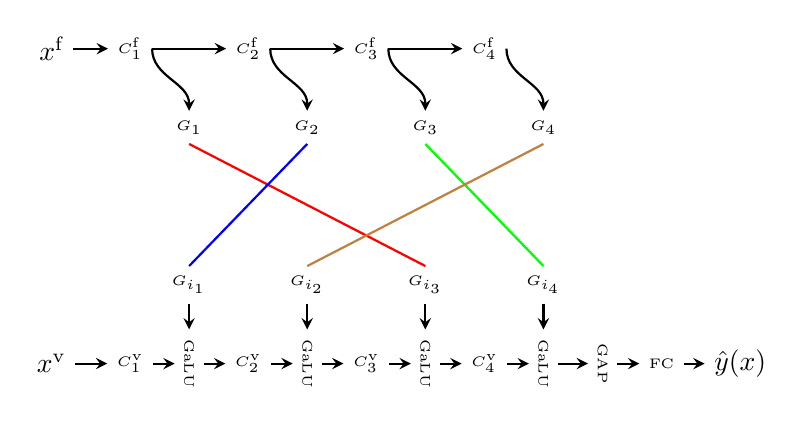
\begin{tikzpicture}
%\node []  (fntext)at (-4.625,-3.5) {CNN-GAP-DLGN};

%\node []  (output) at (7.5,1.5) {$\hat{y}(x)$};


\node [] (dgn1-f-c4) at (-3.5,1.5){\tiny{$C^{\text{f}}_4$}};
\node [] (dgn1-f-c3) at (-5,1.5){\tiny{$C^{\text{f}}_3$}};
\node [] (dgn1-f-c2) at (-6.5,1.5){\tiny{$C^{\text{f}}_2$}};
\node [] (dgn1-f-c1) at (-8,1.5){\tiny{$C^{\text{f}}_1$}};
\node [] (dgn1-input-f) at (-9,1.5){$x^{\text{f}}$};
\draw [-stealth,thick]   (dgn1-f-c3.east) -- (dgn1-f-c4.west);
\draw [-stealth,thick]   (dgn1-f-c2.east) -- (dgn1-f-c3.west);
\draw [-stealth,thick]   (dgn1-f-c1.east) -- (dgn1-f-c2.west);
\draw [-stealth,thick]   (dgn1-input-f.east) -- (dgn1-f-c1.west);



\node []  (dgn1-output) at (-0.25,-2.5) {$\hat{y}(x)$};

\node [] (dgn1-smax) at (-1.25,-2.5){\tiny{FC}};
\draw [-stealth,thick]   (dgn1-smax.east)--(dgn1-output.west);

\node [rotate=-90] (dgn1-gap) at (-2,-2.5){\tiny{GAP}};
\draw [-stealth,thick]   (dgn1-gap.north)--(dgn1-smax.west);


\node [rotate=-90] (dgn1-galu-4) at (-2.75,-2.5){\tiny{GaLU}};
\draw [-stealth,thick]   (dgn1-galu-4.north)--(dgn1-gap.south);

\node [] (dgn1-v-c4) at (-3.5,-2.5){\tiny{$C^{\text{v}}_4$}};
\draw [-stealth,thick]   (dgn1-v-c4.east) -- (dgn1-galu-4.south);


\node [rotate=-90] (dgn1-galu-3) at (-4.25,-2.5){\tiny{GaLU}};
\draw [-stealth,thick]   (dgn1-galu-3.north) -- (dgn1-v-c4.west);

\node [] (dgn1-v-c3) at (-5,-2.5){\tiny{$C^{\text{v}}_3$}};
\draw [-stealth,thick]   (dgn1-v-c3.east) -- (dgn1-galu-3.south);


\node [rotate=-90] (dgn1-galu-2) at (-5.75,-2.5){\tiny{GaLU}};
\draw [-stealth,thick]   (dgn1-galu-2.north) -- (dgn1-v-c3.west);

\node [] (dgn1-v-c2) at (-6.5,-2.5){\tiny{$C^{\text{v}}_2$}};
\draw [-stealth,thick]   (dgn1-v-c2.east) -- (dgn1-galu-2.south);


\node [rotate=-90] (dgn1-galu-1) at (-7.25,-2.5){\tiny{GaLU}};
\draw [-stealth,thick]   (dgn1-galu-1.north) -- (dgn1-v-c2.west);


\node [] (dgn1-v-c1) at (-8,-2.5){\tiny{$C^{\text{v}}_1$}};
\draw [-stealth,thick]   (dgn1-v-c1.east) -- (dgn1-galu-1.south);


\node [] (dgn1-v-input) at (-9,-2.5){$x^{\text{v}}$};

\draw [-stealth,thick]   (dgn1-v-input.east) -- (dgn1-v-c1.west);


\node[] (dgn1-gating-4-up) at (-2.75,0.5){\tiny{$G_{4}$}};
\draw [-stealth,thick]   (dgn1-f-c4.east) to[out=-90,in=90] (dgn1-gating-4-up.north);


\node[] (dgn1-gating-3-up) at (-4.25,0.5){\tiny{$G_{3}$}};
\draw [-stealth,thick]   (dgn1-f-c3.east) to[out=-90,in=90] (dgn1-gating-3-up.north);



\node[] (dgn1-gating-2-up) at (-5.75,0.5){\tiny{$G_{2}$}};
\draw [-stealth,thick]   (dgn1-f-c2.east) to[out=-90,in=90] (dgn1-gating-2-up.north);


\node[] (dgn1-gating-1-up) at (-7.25,0.5){\tiny{$G_{1}$}};
\draw [-stealth,thick]   (dgn1-f-c1.east) to[out=-90,in=90] (dgn1-gating-1-up.north);





\node[] (dgn1-gating-4) at (-2.75,-1.5){\tiny{$G_{i_4}$}};
\draw [-stealth,thick]   (dgn1-gating-4.south) -- (dgn1-galu-4.west);


\node[] (dgn1-gating-3) at (-4.25,-1.5){\tiny{$G_{i_3}$}};
\draw [-stealth,thick]   (dgn1-gating-3.south) -- (dgn1-galu-3.west);



\node[] (dgn1-gating-2) at (-5.75,-1.5){\tiny{$G_{i_2}$}};
\draw [-stealth,thick]   (dgn1-gating-2.south) -- (dgn1-galu-2.west);


\node[] (dgn1-gating-1) at (-7.25,-1.5){\tiny{$G_{i_1}$}};
\draw [-stealth,thick]   (dgn1-gating-1.south) -- (dgn1-galu-1.west);



\draw [-,thick,color=red]   (dgn1-gating-1-up.south) --(dgn1-gating-3.north);

\draw [-,thick,color=blue]   (dgn1-gating-2-up.south) --(dgn1-gating-1.north);

\draw [-,thick,color=green]   (dgn1-gating-3-up.south) --(dgn1-gating-4.north);

\draw [-,thick,color=brown]   (dgn1-gating-4-up.south) --(dgn1-gating-2.north);


%%%%%%%%%%%%%%%%%%%%%%%%%%%%%%%%%%%%%%%%%%%%%%%%%%%%%%%%%%%%%%%%%
	
\end{tikzpicture}


}
\end{minipage}
\begin{minipage}{0.48\columnwidth}
\centering
\resizebox{0.99\columnwidth}{!}{
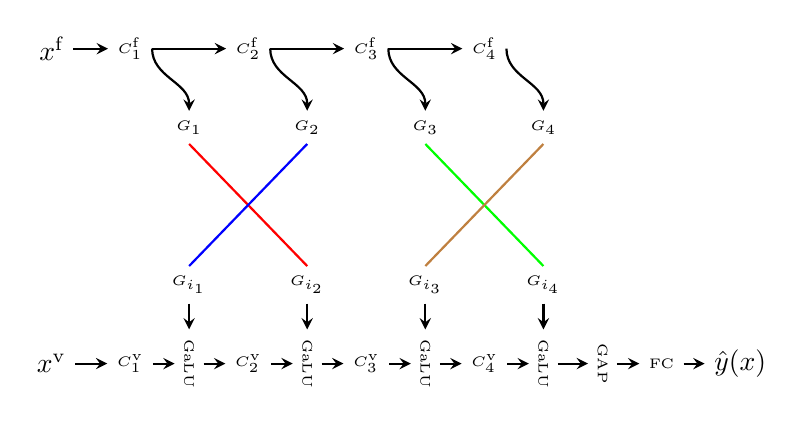
\begin{tikzpicture}
%\node []  (fntext)at (-4.625,-3.5) {CNN-GAP-DLGN};

%\node []  (output) at (7.5,1.5) {$\hat{y}(x)$};


\node [] (dgn1-f-c4) at (-3.5,1.5){\tiny{$C^{\text{f}}_4$}};
\node [] (dgn1-f-c3) at (-5,1.5){\tiny{$C^{\text{f}}_3$}};
\node [] (dgn1-f-c2) at (-6.5,1.5){\tiny{$C^{\text{f}}_2$}};
\node [] (dgn1-f-c1) at (-8,1.5){\tiny{$C^{\text{f}}_1$}};
\node [] (dgn1-input-f) at (-9,1.5){$x^{\text{f}}$};
\draw [-stealth,thick]   (dgn1-f-c3.east) -- (dgn1-f-c4.west);
\draw [-stealth,thick]   (dgn1-f-c2.east) -- (dgn1-f-c3.west);
\draw [-stealth,thick]   (dgn1-f-c1.east) -- (dgn1-f-c2.west);
\draw [-stealth,thick]   (dgn1-input-f.east) -- (dgn1-f-c1.west);



\node []  (dgn1-output) at (-0.25,-2.5) {$\hat{y}(x)$};

\node [] (dgn1-smax) at (-1.25,-2.5){\tiny{FC}};
\draw [-stealth,thick]   (dgn1-smax.east)--(dgn1-output.west);

\node [rotate=-90] (dgn1-gap) at (-2,-2.5){\tiny{GAP}};
\draw [-stealth,thick]   (dgn1-gap.north)--(dgn1-smax.west);


\node [rotate=-90] (dgn1-galu-4) at (-2.75,-2.5){\tiny{GaLU}};
\draw [-stealth,thick]   (dgn1-galu-4.north)--(dgn1-gap.south);

\node [] (dgn1-v-c4) at (-3.5,-2.5){\tiny{$C^{\text{v}}_4$}};
\draw [-stealth,thick]   (dgn1-v-c4.east) -- (dgn1-galu-4.south);


\node [rotate=-90] (dgn1-galu-3) at (-4.25,-2.5){\tiny{GaLU}};
\draw [-stealth,thick]   (dgn1-galu-3.north) -- (dgn1-v-c4.west);

\node [] (dgn1-v-c3) at (-5,-2.5){\tiny{$C^{\text{v}}_3$}};
\draw [-stealth,thick]   (dgn1-v-c3.east) -- (dgn1-galu-3.south);


\node [rotate=-90] (dgn1-galu-2) at (-5.75,-2.5){\tiny{GaLU}};
\draw [-stealth,thick]   (dgn1-galu-2.north) -- (dgn1-v-c3.west);

\node [] (dgn1-v-c2) at (-6.5,-2.5){\tiny{$C^{\text{v}}_2$}};
\draw [-stealth,thick]   (dgn1-v-c2.east) -- (dgn1-galu-2.south);


\node [rotate=-90] (dgn1-galu-1) at (-7.25,-2.5){\tiny{GaLU}};
\draw [-stealth,thick]   (dgn1-galu-1.north) -- (dgn1-v-c2.west);


\node [] (dgn1-v-c1) at (-8,-2.5){\tiny{$C^{\text{v}}_1$}};
\draw [-stealth,thick]   (dgn1-v-c1.east) -- (dgn1-galu-1.south);


\node [] (dgn1-v-input) at (-9,-2.5){$x^{\text{v}}$};

\draw [-stealth,thick]   (dgn1-v-input.east) -- (dgn1-v-c1.west);


\node[] (dgn1-gating-4-up) at (-2.75,0.5){\tiny{$G_{4}$}};
\draw [-stealth,thick]   (dgn1-f-c4.east) to[out=-90,in=90] (dgn1-gating-4-up.north);


\node[] (dgn1-gating-3-up) at (-4.25,0.5){\tiny{$G_{3}$}};
\draw [-stealth,thick]   (dgn1-f-c3.east) to[out=-90,in=90] (dgn1-gating-3-up.north);



\node[] (dgn1-gating-2-up) at (-5.75,0.5){\tiny{$G_{2}$}};
\draw [-stealth,thick]   (dgn1-f-c2.east) to[out=-90,in=90] (dgn1-gating-2-up.north);


\node[] (dgn1-gating-1-up) at (-7.25,0.5){\tiny{$G_{1}$}};
\draw [-stealth,thick]   (dgn1-f-c1.east) to[out=-90,in=90] (dgn1-gating-1-up.north);





\node[] (dgn1-gating-4) at (-2.75,-1.5){\tiny{$G_{i_4}$}};
\draw [-stealth,thick]   (dgn1-gating-4.south) -- (dgn1-galu-4.west);


\node[] (dgn1-gating-3) at (-4.25,-1.5){\tiny{$G_{i_3}$}};
\draw [-stealth,thick]   (dgn1-gating-3.south) -- (dgn1-galu-3.west);



\node[] (dgn1-gating-2) at (-5.75,-1.5){\tiny{$G_{i_2}$}};
\draw [-stealth,thick]   (dgn1-gating-2.south) -- (dgn1-galu-2.west);


\node[] (dgn1-gating-1) at (-7.25,-1.5){\tiny{$G_{i_1}$}};
\draw [-stealth,thick]   (dgn1-gating-1.south) -- (dgn1-galu-1.west);



\draw [-,thick,color=red]   (dgn1-gating-1-up.south) --(dgn1-gating-2.north);

\draw [-,thick,color=blue]   (dgn1-gating-2-up.south) --(dgn1-gating-1.north);

\draw [-,thick,color=green]   (dgn1-gating-3-up.south) --(dgn1-gating-4.north);

\draw [-,thick,color=brown]   (dgn1-gating-4-up.south) --(dgn1-gating-3.north);


%%%%%%%%%%%%%%%%%%%%%%%%%%%%%%%%%%%%%%%%%%%%%%%%%%%%%%%%%%%%%%%%%
	
\end{tikzpicture}


}
\end{minipage}



\begin{minipage}{0.48\columnwidth}
\centering
\resizebox{0.99\columnwidth}{!}{
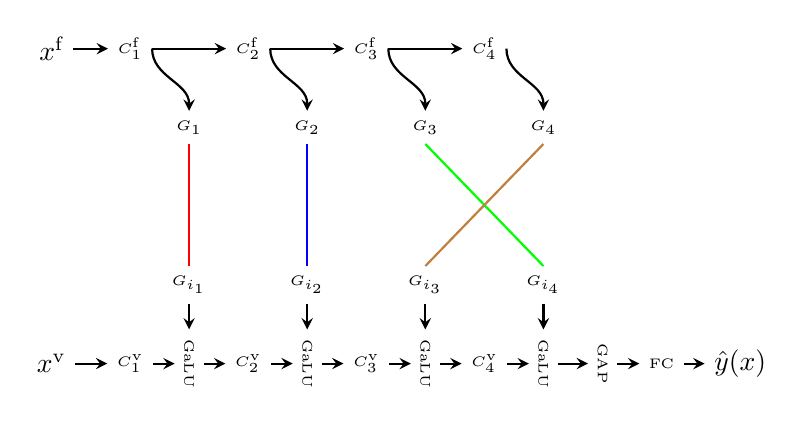
\begin{tikzpicture}
%\node []  (fntext)at (-4.625,-3.5) {CNN-GAP-DLGN};

%\node []  (output) at (7.5,1.5) {$\hat{y}(x)$};


\node [] (dgn1-f-c4) at (-3.5,1.5){\tiny{$C^{\text{f}}_4$}};
\node [] (dgn1-f-c3) at (-5,1.5){\tiny{$C^{\text{f}}_3$}};
\node [] (dgn1-f-c2) at (-6.5,1.5){\tiny{$C^{\text{f}}_2$}};
\node [] (dgn1-f-c1) at (-8,1.5){\tiny{$C^{\text{f}}_1$}};
\node [] (dgn1-input-f) at (-9,1.5){$x^{\text{f}}$};
\draw [-stealth,thick]   (dgn1-f-c3.east) -- (dgn1-f-c4.west);
\draw [-stealth,thick]   (dgn1-f-c2.east) -- (dgn1-f-c3.west);
\draw [-stealth,thick]   (dgn1-f-c1.east) -- (dgn1-f-c2.west);
\draw [-stealth,thick]   (dgn1-input-f.east) -- (dgn1-f-c1.west);



\node []  (dgn1-output) at (-0.25,-2.5) {$\hat{y}(x)$};

\node [] (dgn1-smax) at (-1.25,-2.5){\tiny{FC}};
\draw [-stealth,thick]   (dgn1-smax.east)--(dgn1-output.west);

\node [rotate=-90] (dgn1-gap) at (-2,-2.5){\tiny{GAP}};
\draw [-stealth,thick]   (dgn1-gap.north)--(dgn1-smax.west);


\node [rotate=-90] (dgn1-galu-4) at (-2.75,-2.5){\tiny{GaLU}};
\draw [-stealth,thick]   (dgn1-galu-4.north)--(dgn1-gap.south);

\node [] (dgn1-v-c4) at (-3.5,-2.5){\tiny{$C^{\text{v}}_4$}};
\draw [-stealth,thick]   (dgn1-v-c4.east) -- (dgn1-galu-4.south);


\node [rotate=-90] (dgn1-galu-3) at (-4.25,-2.5){\tiny{GaLU}};
\draw [-stealth,thick]   (dgn1-galu-3.north) -- (dgn1-v-c4.west);

\node [] (dgn1-v-c3) at (-5,-2.5){\tiny{$C^{\text{v}}_3$}};
\draw [-stealth,thick]   (dgn1-v-c3.east) -- (dgn1-galu-3.south);


\node [rotate=-90] (dgn1-galu-2) at (-5.75,-2.5){\tiny{GaLU}};
\draw [-stealth,thick]   (dgn1-galu-2.north) -- (dgn1-v-c3.west);

\node [] (dgn1-v-c2) at (-6.5,-2.5){\tiny{$C^{\text{v}}_2$}};
\draw [-stealth,thick]   (dgn1-v-c2.east) -- (dgn1-galu-2.south);


\node [rotate=-90] (dgn1-galu-1) at (-7.25,-2.5){\tiny{GaLU}};
\draw [-stealth,thick]   (dgn1-galu-1.north) -- (dgn1-v-c2.west);


\node [] (dgn1-v-c1) at (-8,-2.5){\tiny{$C^{\text{v}}_1$}};
\draw [-stealth,thick]   (dgn1-v-c1.east) -- (dgn1-galu-1.south);


\node [] (dgn1-v-input) at (-9,-2.5){$x^{\text{v}}$};

\draw [-stealth,thick]   (dgn1-v-input.east) -- (dgn1-v-c1.west);


\node[] (dgn1-gating-4-up) at (-2.75,0.5){\tiny{$G_{4}$}};
\draw [-stealth,thick]   (dgn1-f-c4.east) to[out=-90,in=90] (dgn1-gating-4-up.north);


\node[] (dgn1-gating-3-up) at (-4.25,0.5){\tiny{$G_{3}$}};
\draw [-stealth,thick]   (dgn1-f-c3.east) to[out=-90,in=90] (dgn1-gating-3-up.north);



\node[] (dgn1-gating-2-up) at (-5.75,0.5){\tiny{$G_{2}$}};
\draw [-stealth,thick]   (dgn1-f-c2.east) to[out=-90,in=90] (dgn1-gating-2-up.north);


\node[] (dgn1-gating-1-up) at (-7.25,0.5){\tiny{$G_{1}$}};
\draw [-stealth,thick]   (dgn1-f-c1.east) to[out=-90,in=90] (dgn1-gating-1-up.north);





\node[] (dgn1-gating-4) at (-2.75,-1.5){\tiny{$G_{i_4}$}};
\draw [-stealth,thick]   (dgn1-gating-4.south) -- (dgn1-galu-4.west);


\node[] (dgn1-gating-3) at (-4.25,-1.5){\tiny{$G_{i_3}$}};
\draw [-stealth,thick]   (dgn1-gating-3.south) -- (dgn1-galu-3.west);



\node[] (dgn1-gating-2) at (-5.75,-1.5){\tiny{$G_{i_2}$}};
\draw [-stealth,thick]   (dgn1-gating-2.south) -- (dgn1-galu-2.west);


\node[] (dgn1-gating-1) at (-7.25,-1.5){\tiny{$G_{i_1}$}};
\draw [-stealth,thick]   (dgn1-gating-1.south) -- (dgn1-galu-1.west);



\draw [-,thick,color=red]   (dgn1-gating-1-up.south) --(dgn1-gating-1.north);

\draw [-,thick,color=blue]   (dgn1-gating-2-up.south) --(dgn1-gating-2.north);

\draw [-,thick,color=green]   (dgn1-gating-3-up.south) --(dgn1-gating-4.north);

\draw [-,thick,color=brown]   (dgn1-gating-4-up.south) --(dgn1-gating-3.north);


%%%%%%%%%%%%%%%%%%%%%%%%%%%%%%%%%%%%%%%%%%%%%%%%%%%%%%%%%%%%%%%%%
	
\end{tikzpicture}


}
\end{minipage}
\begin{minipage}{0.48\columnwidth}
\centering
\resizebox{0.99\columnwidth}{!}{
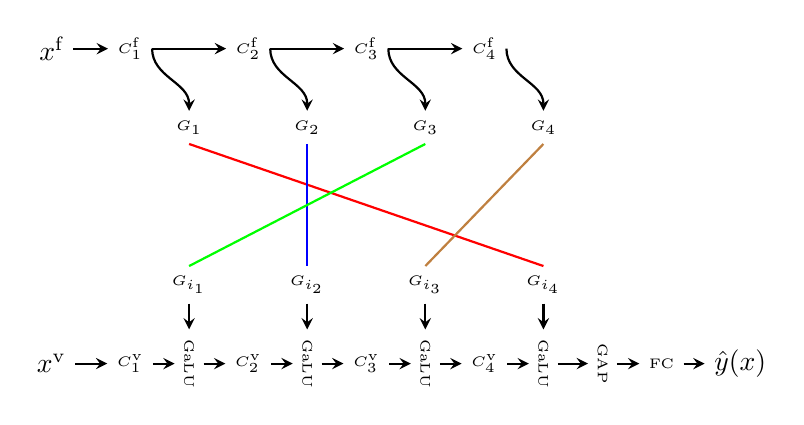
\begin{tikzpicture}
%\node []  (fntext)at (-4.625,-3.5) {CNN-GAP-DLGN};

%\node []  (output) at (7.5,1.5) {$\hat{y}(x)$};


\node [] (dgn1-f-c4) at (-3.5,1.5){\tiny{$C^{\text{f}}_4$}};
\node [] (dgn1-f-c3) at (-5,1.5){\tiny{$C^{\text{f}}_3$}};
\node [] (dgn1-f-c2) at (-6.5,1.5){\tiny{$C^{\text{f}}_2$}};
\node [] (dgn1-f-c1) at (-8,1.5){\tiny{$C^{\text{f}}_1$}};
\node [] (dgn1-input-f) at (-9,1.5){$x^{\text{f}}$};
\draw [-stealth,thick]   (dgn1-f-c3.east) -- (dgn1-f-c4.west);
\draw [-stealth,thick]   (dgn1-f-c2.east) -- (dgn1-f-c3.west);
\draw [-stealth,thick]   (dgn1-f-c1.east) -- (dgn1-f-c2.west);
\draw [-stealth,thick]   (dgn1-input-f.east) -- (dgn1-f-c1.west);



\node []  (dgn1-output) at (-0.25,-2.5) {$\hat{y}(x)$};

\node [] (dgn1-smax) at (-1.25,-2.5){\tiny{FC}};
\draw [-stealth,thick]   (dgn1-smax.east)--(dgn1-output.west);

\node [rotate=-90] (dgn1-gap) at (-2,-2.5){\tiny{GAP}};
\draw [-stealth,thick]   (dgn1-gap.north)--(dgn1-smax.west);


\node [rotate=-90] (dgn1-galu-4) at (-2.75,-2.5){\tiny{GaLU}};
\draw [-stealth,thick]   (dgn1-galu-4.north)--(dgn1-gap.south);

\node [] (dgn1-v-c4) at (-3.5,-2.5){\tiny{$C^{\text{v}}_4$}};
\draw [-stealth,thick]   (dgn1-v-c4.east) -- (dgn1-galu-4.south);


\node [rotate=-90] (dgn1-galu-3) at (-4.25,-2.5){\tiny{GaLU}};
\draw [-stealth,thick]   (dgn1-galu-3.north) -- (dgn1-v-c4.west);

\node [] (dgn1-v-c3) at (-5,-2.5){\tiny{$C^{\text{v}}_3$}};
\draw [-stealth,thick]   (dgn1-v-c3.east) -- (dgn1-galu-3.south);


\node [rotate=-90] (dgn1-galu-2) at (-5.75,-2.5){\tiny{GaLU}};
\draw [-stealth,thick]   (dgn1-galu-2.north) -- (dgn1-v-c3.west);

\node [] (dgn1-v-c2) at (-6.5,-2.5){\tiny{$C^{\text{v}}_2$}};
\draw [-stealth,thick]   (dgn1-v-c2.east) -- (dgn1-galu-2.south);


\node [rotate=-90] (dgn1-galu-1) at (-7.25,-2.5){\tiny{GaLU}};
\draw [-stealth,thick]   (dgn1-galu-1.north) -- (dgn1-v-c2.west);


\node [] (dgn1-v-c1) at (-8,-2.5){\tiny{$C^{\text{v}}_1$}};
\draw [-stealth,thick]   (dgn1-v-c1.east) -- (dgn1-galu-1.south);


\node [] (dgn1-v-input) at (-9,-2.5){$x^{\text{v}}$};

\draw [-stealth,thick]   (dgn1-v-input.east) -- (dgn1-v-c1.west);


\node[] (dgn1-gating-4-up) at (-2.75,0.5){\tiny{$G_{4}$}};
\draw [-stealth,thick]   (dgn1-f-c4.east) to[out=-90,in=90] (dgn1-gating-4-up.north);


\node[] (dgn1-gating-3-up) at (-4.25,0.5){\tiny{$G_{3}$}};
\draw [-stealth,thick]   (dgn1-f-c3.east) to[out=-90,in=90] (dgn1-gating-3-up.north);



\node[] (dgn1-gating-2-up) at (-5.75,0.5){\tiny{$G_{2}$}};
\draw [-stealth,thick]   (dgn1-f-c2.east) to[out=-90,in=90] (dgn1-gating-2-up.north);


\node[] (dgn1-gating-1-up) at (-7.25,0.5){\tiny{$G_{1}$}};
\draw [-stealth,thick]   (dgn1-f-c1.east) to[out=-90,in=90] (dgn1-gating-1-up.north);





\node[] (dgn1-gating-4) at (-2.75,-1.5){\tiny{$G_{i_4}$}};
\draw [-stealth,thick]   (dgn1-gating-4.south) -- (dgn1-galu-4.west);


\node[] (dgn1-gating-3) at (-4.25,-1.5){\tiny{$G_{i_3}$}};
\draw [-stealth,thick]   (dgn1-gating-3.south) -- (dgn1-galu-3.west);



\node[] (dgn1-gating-2) at (-5.75,-1.5){\tiny{$G_{i_2}$}};
\draw [-stealth,thick]   (dgn1-gating-2.south) -- (dgn1-galu-2.west);


\node[] (dgn1-gating-1) at (-7.25,-1.5){\tiny{$G_{i_1}$}};
\draw [-stealth,thick]   (dgn1-gating-1.south) -- (dgn1-galu-1.west);



\draw [-,thick,color=red]   (dgn1-gating-1-up.south) --(dgn1-gating-4.north);

\draw [-,thick,color=blue]   (dgn1-gating-2-up.south) --(dgn1-gating-2.north);

\draw [-,thick,color=green]   (dgn1-gating-3-up.south) --(dgn1-gating-1.north);

\draw [-,thick,color=brown]   (dgn1-gating-4-up.south) --(dgn1-gating-3.north);


%%%%%%%%%%%%%%%%%%%%%%%%%%%%%%%%%%%%%%%%%%%%%%%%%%%%%%%%%%%%%%%%%
	
\end{tikzpicture}


}
\end{minipage}

\begin{minipage}{0.48\columnwidth}
\centering
\resizebox{0.99\columnwidth}{!}{
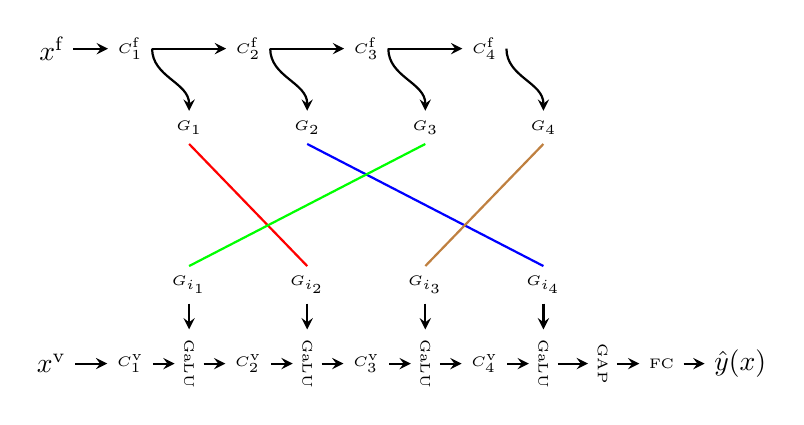
\begin{tikzpicture}
%\node []  (fntext)at (-4.625,-3.5) {CNN-GAP-DLGN};

%\node []  (output) at (7.5,1.5) {$\hat{y}(x)$};


\node [] (dgn1-f-c4) at (-3.5,1.5){\tiny{$C^{\text{f}}_4$}};
\node [] (dgn1-f-c3) at (-5,1.5){\tiny{$C^{\text{f}}_3$}};
\node [] (dgn1-f-c2) at (-6.5,1.5){\tiny{$C^{\text{f}}_2$}};
\node [] (dgn1-f-c1) at (-8,1.5){\tiny{$C^{\text{f}}_1$}};
\node [] (dgn1-input-f) at (-9,1.5){$x^{\text{f}}$};
\draw [-stealth,thick]   (dgn1-f-c3.east) -- (dgn1-f-c4.west);
\draw [-stealth,thick]   (dgn1-f-c2.east) -- (dgn1-f-c3.west);
\draw [-stealth,thick]   (dgn1-f-c1.east) -- (dgn1-f-c2.west);
\draw [-stealth,thick]   (dgn1-input-f.east) -- (dgn1-f-c1.west);



\node []  (dgn1-output) at (-0.25,-2.5) {$\hat{y}(x)$};

\node [] (dgn1-smax) at (-1.25,-2.5){\tiny{FC}};
\draw [-stealth,thick]   (dgn1-smax.east)--(dgn1-output.west);

\node [rotate=-90] (dgn1-gap) at (-2,-2.5){\tiny{GAP}};
\draw [-stealth,thick]   (dgn1-gap.north)--(dgn1-smax.west);


\node [rotate=-90] (dgn1-galu-4) at (-2.75,-2.5){\tiny{GaLU}};
\draw [-stealth,thick]   (dgn1-galu-4.north)--(dgn1-gap.south);

\node [] (dgn1-v-c4) at (-3.5,-2.5){\tiny{$C^{\text{v}}_4$}};
\draw [-stealth,thick]   (dgn1-v-c4.east) -- (dgn1-galu-4.south);


\node [rotate=-90] (dgn1-galu-3) at (-4.25,-2.5){\tiny{GaLU}};
\draw [-stealth,thick]   (dgn1-galu-3.north) -- (dgn1-v-c4.west);

\node [] (dgn1-v-c3) at (-5,-2.5){\tiny{$C^{\text{v}}_3$}};
\draw [-stealth,thick]   (dgn1-v-c3.east) -- (dgn1-galu-3.south);


\node [rotate=-90] (dgn1-galu-2) at (-5.75,-2.5){\tiny{GaLU}};
\draw [-stealth,thick]   (dgn1-galu-2.north) -- (dgn1-v-c3.west);

\node [] (dgn1-v-c2) at (-6.5,-2.5){\tiny{$C^{\text{v}}_2$}};
\draw [-stealth,thick]   (dgn1-v-c2.east) -- (dgn1-galu-2.south);


\node [rotate=-90] (dgn1-galu-1) at (-7.25,-2.5){\tiny{GaLU}};
\draw [-stealth,thick]   (dgn1-galu-1.north) -- (dgn1-v-c2.west);


\node [] (dgn1-v-c1) at (-8,-2.5){\tiny{$C^{\text{v}}_1$}};
\draw [-stealth,thick]   (dgn1-v-c1.east) -- (dgn1-galu-1.south);


\node [] (dgn1-v-input) at (-9,-2.5){$x^{\text{v}}$};

\draw [-stealth,thick]   (dgn1-v-input.east) -- (dgn1-v-c1.west);


\node[] (dgn1-gating-4-up) at (-2.75,0.5){\tiny{$G_{4}$}};
\draw [-stealth,thick]   (dgn1-f-c4.east) to[out=-90,in=90] (dgn1-gating-4-up.north);


\node[] (dgn1-gating-3-up) at (-4.25,0.5){\tiny{$G_{3}$}};
\draw [-stealth,thick]   (dgn1-f-c3.east) to[out=-90,in=90] (dgn1-gating-3-up.north);



\node[] (dgn1-gating-2-up) at (-5.75,0.5){\tiny{$G_{2}$}};
\draw [-stealth,thick]   (dgn1-f-c2.east) to[out=-90,in=90] (dgn1-gating-2-up.north);


\node[] (dgn1-gating-1-up) at (-7.25,0.5){\tiny{$G_{1}$}};
\draw [-stealth,thick]   (dgn1-f-c1.east) to[out=-90,in=90] (dgn1-gating-1-up.north);





\node[] (dgn1-gating-4) at (-2.75,-1.5){\tiny{$G_{i_4}$}};
\draw [-stealth,thick]   (dgn1-gating-4.south) -- (dgn1-galu-4.west);


\node[] (dgn1-gating-3) at (-4.25,-1.5){\tiny{$G_{i_3}$}};
\draw [-stealth,thick]   (dgn1-gating-3.south) -- (dgn1-galu-3.west);



\node[] (dgn1-gating-2) at (-5.75,-1.5){\tiny{$G_{i_2}$}};
\draw [-stealth,thick]   (dgn1-gating-2.south) -- (dgn1-galu-2.west);


\node[] (dgn1-gating-1) at (-7.25,-1.5){\tiny{$G_{i_1}$}};
\draw [-stealth,thick]   (dgn1-gating-1.south) -- (dgn1-galu-1.west);



\draw [-,thick,color=red]   (dgn1-gating-1-up.south) --(dgn1-gating-2.north);

\draw [-,thick,color=blue]   (dgn1-gating-2-up.south) --(dgn1-gating-4.north);

\draw [-,thick,color=green]   (dgn1-gating-3-up.south) --(dgn1-gating-1.north);

\draw [-,thick,color=brown]   (dgn1-gating-4-up.south) --(dgn1-gating-3.north);


%%%%%%%%%%%%%%%%%%%%%%%%%%%%%%%%%%%%%%%%%%%%%%%%%%%%%%%%%%%%%%%%%
	
\end{tikzpicture}


}
\end{minipage}
\begin{minipage}{0.48\columnwidth}
\centering
\resizebox{0.99\columnwidth}{!}{
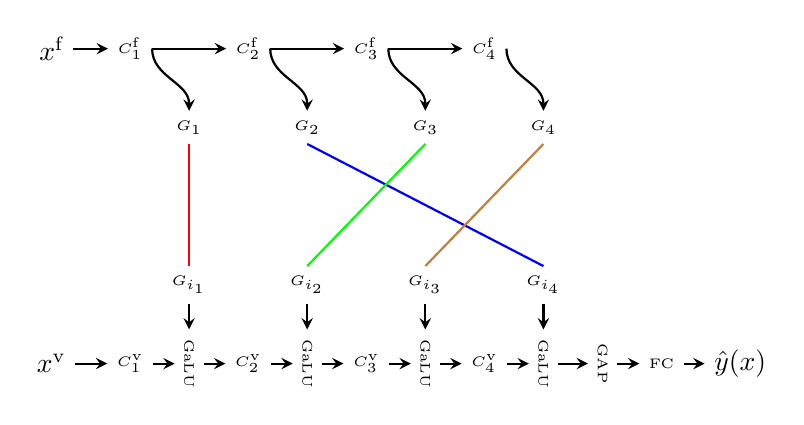
\begin{tikzpicture}
%\node []  (fntext)at (-4.625,-3.5) {CNN-GAP-DLGN};

%\node []  (output) at (7.5,1.5) {$\hat{y}(x)$};


\node [] (dgn1-f-c4) at (-3.5,1.5){\tiny{$C^{\text{f}}_4$}};
\node [] (dgn1-f-c3) at (-5,1.5){\tiny{$C^{\text{f}}_3$}};
\node [] (dgn1-f-c2) at (-6.5,1.5){\tiny{$C^{\text{f}}_2$}};
\node [] (dgn1-f-c1) at (-8,1.5){\tiny{$C^{\text{f}}_1$}};
\node [] (dgn1-input-f) at (-9,1.5){$x^{\text{f}}$};
\draw [-stealth,thick]   (dgn1-f-c3.east) -- (dgn1-f-c4.west);
\draw [-stealth,thick]   (dgn1-f-c2.east) -- (dgn1-f-c3.west);
\draw [-stealth,thick]   (dgn1-f-c1.east) -- (dgn1-f-c2.west);
\draw [-stealth,thick]   (dgn1-input-f.east) -- (dgn1-f-c1.west);



\node []  (dgn1-output) at (-0.25,-2.5) {$\hat{y}(x)$};

\node [] (dgn1-smax) at (-1.25,-2.5){\tiny{FC}};
\draw [-stealth,thick]   (dgn1-smax.east)--(dgn1-output.west);

\node [rotate=-90] (dgn1-gap) at (-2,-2.5){\tiny{GAP}};
\draw [-stealth,thick]   (dgn1-gap.north)--(dgn1-smax.west);


\node [rotate=-90] (dgn1-galu-4) at (-2.75,-2.5){\tiny{GaLU}};
\draw [-stealth,thick]   (dgn1-galu-4.north)--(dgn1-gap.south);

\node [] (dgn1-v-c4) at (-3.5,-2.5){\tiny{$C^{\text{v}}_4$}};
\draw [-stealth,thick]   (dgn1-v-c4.east) -- (dgn1-galu-4.south);


\node [rotate=-90] (dgn1-galu-3) at (-4.25,-2.5){\tiny{GaLU}};
\draw [-stealth,thick]   (dgn1-galu-3.north) -- (dgn1-v-c4.west);

\node [] (dgn1-v-c3) at (-5,-2.5){\tiny{$C^{\text{v}}_3$}};
\draw [-stealth,thick]   (dgn1-v-c3.east) -- (dgn1-galu-3.south);


\node [rotate=-90] (dgn1-galu-2) at (-5.75,-2.5){\tiny{GaLU}};
\draw [-stealth,thick]   (dgn1-galu-2.north) -- (dgn1-v-c3.west);

\node [] (dgn1-v-c2) at (-6.5,-2.5){\tiny{$C^{\text{v}}_2$}};
\draw [-stealth,thick]   (dgn1-v-c2.east) -- (dgn1-galu-2.south);


\node [rotate=-90] (dgn1-galu-1) at (-7.25,-2.5){\tiny{GaLU}};
\draw [-stealth,thick]   (dgn1-galu-1.north) -- (dgn1-v-c2.west);


\node [] (dgn1-v-c1) at (-8,-2.5){\tiny{$C^{\text{v}}_1$}};
\draw [-stealth,thick]   (dgn1-v-c1.east) -- (dgn1-galu-1.south);


\node [] (dgn1-v-input) at (-9,-2.5){$x^{\text{v}}$};

\draw [-stealth,thick]   (dgn1-v-input.east) -- (dgn1-v-c1.west);


\node[] (dgn1-gating-4-up) at (-2.75,0.5){\tiny{$G_{4}$}};
\draw [-stealth,thick]   (dgn1-f-c4.east) to[out=-90,in=90] (dgn1-gating-4-up.north);


\node[] (dgn1-gating-3-up) at (-4.25,0.5){\tiny{$G_{3}$}};
\draw [-stealth,thick]   (dgn1-f-c3.east) to[out=-90,in=90] (dgn1-gating-3-up.north);



\node[] (dgn1-gating-2-up) at (-5.75,0.5){\tiny{$G_{2}$}};
\draw [-stealth,thick]   (dgn1-f-c2.east) to[out=-90,in=90] (dgn1-gating-2-up.north);


\node[] (dgn1-gating-1-up) at (-7.25,0.5){\tiny{$G_{1}$}};
\draw [-stealth,thick]   (dgn1-f-c1.east) to[out=-90,in=90] (dgn1-gating-1-up.north);





\node[] (dgn1-gating-4) at (-2.75,-1.5){\tiny{$G_{i_4}$}};
\draw [-stealth,thick]   (dgn1-gating-4.south) -- (dgn1-galu-4.west);


\node[] (dgn1-gating-3) at (-4.25,-1.5){\tiny{$G_{i_3}$}};
\draw [-stealth,thick]   (dgn1-gating-3.south) -- (dgn1-galu-3.west);



\node[] (dgn1-gating-2) at (-5.75,-1.5){\tiny{$G_{i_2}$}};
\draw [-stealth,thick]   (dgn1-gating-2.south) -- (dgn1-galu-2.west);


\node[] (dgn1-gating-1) at (-7.25,-1.5){\tiny{$G_{i_1}$}};
\draw [-stealth,thick]   (dgn1-gating-1.south) -- (dgn1-galu-1.west);



\draw [-,thick,color=red]   (dgn1-gating-1-up.south) --(dgn1-gating-1.north);

\draw [-,thick,color=blue]   (dgn1-gating-2-up.south) --(dgn1-gating-4.north);

\draw [-,thick,color=green]   (dgn1-gating-3-up.south) --(dgn1-gating-2.north);

\draw [-,thick,color=brown]   (dgn1-gating-4-up.south) --(dgn1-gating-3.north);


%%%%%%%%%%%%%%%%%%%%%%%%%%%%%%%%%%%%%%%%%%%%%%%%%%%%%%%%%%%%%%%%%
	
\end{tikzpicture}


}
\end{minipage}

\begin{minipage}{0.48\columnwidth}
\centering
\resizebox{0.99\columnwidth}{!}{
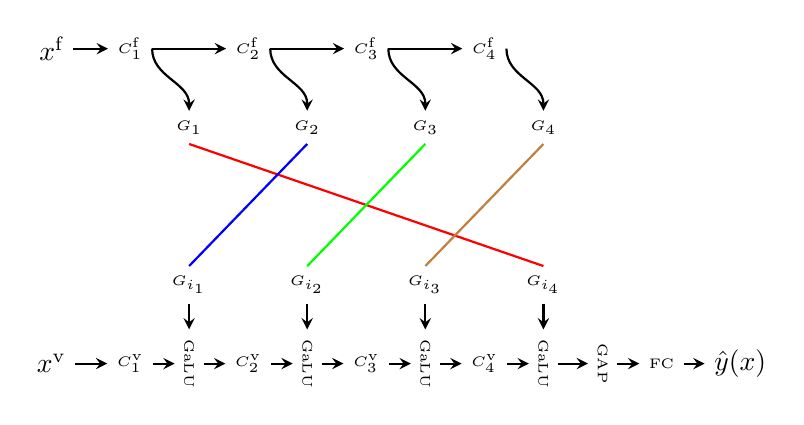
\begin{tikzpicture}
%\node []  (fntext)at (-4.625,-3.5) {CNN-GAP-DLGN};

%\node []  (output) at (7.5,1.5) {$\hat{y}(x)$};


\node [] (dgn1-f-c4) at (-3.5,1.5){\tiny{$C^{\text{f}}_4$}};
\node [] (dgn1-f-c3) at (-5,1.5){\tiny{$C^{\text{f}}_3$}};
\node [] (dgn1-f-c2) at (-6.5,1.5){\tiny{$C^{\text{f}}_2$}};
\node [] (dgn1-f-c1) at (-8,1.5){\tiny{$C^{\text{f}}_1$}};
\node [] (dgn1-input-f) at (-9,1.5){$x^{\text{f}}$};
\draw [-stealth,thick]   (dgn1-f-c3.east) -- (dgn1-f-c4.west);
\draw [-stealth,thick]   (dgn1-f-c2.east) -- (dgn1-f-c3.west);
\draw [-stealth,thick]   (dgn1-f-c1.east) -- (dgn1-f-c2.west);
\draw [-stealth,thick]   (dgn1-input-f.east) -- (dgn1-f-c1.west);



\node []  (dgn1-output) at (-0.25,-2.5) {$\hat{y}(x)$};

\node [] (dgn1-smax) at (-1.25,-2.5){\tiny{FC}};
\draw [-stealth,thick]   (dgn1-smax.east)--(dgn1-output.west);

\node [rotate=-90] (dgn1-gap) at (-2,-2.5){\tiny{GAP}};
\draw [-stealth,thick]   (dgn1-gap.north)--(dgn1-smax.west);


\node [rotate=-90] (dgn1-galu-4) at (-2.75,-2.5){\tiny{GaLU}};
\draw [-stealth,thick]   (dgn1-galu-4.north)--(dgn1-gap.south);

\node [] (dgn1-v-c4) at (-3.5,-2.5){\tiny{$C^{\text{v}}_4$}};
\draw [-stealth,thick]   (dgn1-v-c4.east) -- (dgn1-galu-4.south);


\node [rotate=-90] (dgn1-galu-3) at (-4.25,-2.5){\tiny{GaLU}};
\draw [-stealth,thick]   (dgn1-galu-3.north) -- (dgn1-v-c4.west);

\node [] (dgn1-v-c3) at (-5,-2.5){\tiny{$C^{\text{v}}_3$}};
\draw [-stealth,thick]   (dgn1-v-c3.east) -- (dgn1-galu-3.south);


\node [rotate=-90] (dgn1-galu-2) at (-5.75,-2.5){\tiny{GaLU}};
\draw [-stealth,thick]   (dgn1-galu-2.north) -- (dgn1-v-c3.west);

\node [] (dgn1-v-c2) at (-6.5,-2.5){\tiny{$C^{\text{v}}_2$}};
\draw [-stealth,thick]   (dgn1-v-c2.east) -- (dgn1-galu-2.south);


\node [rotate=-90] (dgn1-galu-1) at (-7.25,-2.5){\tiny{GaLU}};
\draw [-stealth,thick]   (dgn1-galu-1.north) -- (dgn1-v-c2.west);


\node [] (dgn1-v-c1) at (-8,-2.5){\tiny{$C^{\text{v}}_1$}};
\draw [-stealth,thick]   (dgn1-v-c1.east) -- (dgn1-galu-1.south);


\node [] (dgn1-v-input) at (-9,-2.5){$x^{\text{v}}$};

\draw [-stealth,thick]   (dgn1-v-input.east) -- (dgn1-v-c1.west);


\node[] (dgn1-gating-4-up) at (-2.75,0.5){\tiny{$G_{4}$}};
\draw [-stealth,thick]   (dgn1-f-c4.east) to[out=-90,in=90] (dgn1-gating-4-up.north);


\node[] (dgn1-gating-3-up) at (-4.25,0.5){\tiny{$G_{3}$}};
\draw [-stealth,thick]   (dgn1-f-c3.east) to[out=-90,in=90] (dgn1-gating-3-up.north);



\node[] (dgn1-gating-2-up) at (-5.75,0.5){\tiny{$G_{2}$}};
\draw [-stealth,thick]   (dgn1-f-c2.east) to[out=-90,in=90] (dgn1-gating-2-up.north);


\node[] (dgn1-gating-1-up) at (-7.25,0.5){\tiny{$G_{1}$}};
\draw [-stealth,thick]   (dgn1-f-c1.east) to[out=-90,in=90] (dgn1-gating-1-up.north);





\node[] (dgn1-gating-4) at (-2.75,-1.5){\tiny{$G_{i_4}$}};
\draw [-stealth,thick]   (dgn1-gating-4.south) -- (dgn1-galu-4.west);


\node[] (dgn1-gating-3) at (-4.25,-1.5){\tiny{$G_{i_3}$}};
\draw [-stealth,thick]   (dgn1-gating-3.south) -- (dgn1-galu-3.west);



\node[] (dgn1-gating-2) at (-5.75,-1.5){\tiny{$G_{i_2}$}};
\draw [-stealth,thick]   (dgn1-gating-2.south) -- (dgn1-galu-2.west);


\node[] (dgn1-gating-1) at (-7.25,-1.5){\tiny{$G_{i_1}$}};
\draw [-stealth,thick]   (dgn1-gating-1.south) -- (dgn1-galu-1.west);



\draw [-,thick,color=red]   (dgn1-gating-1-up.south) --(dgn1-gating-4.north);

\draw [-,thick,color=blue]   (dgn1-gating-2-up.south) --(dgn1-gating-1.north);

\draw [-,thick,color=green]   (dgn1-gating-3-up.south) --(dgn1-gating-2.north);

\draw [-,thick,color=brown]   (dgn1-gating-4-up.south) --(dgn1-gating-3.north);


%%%%%%%%%%%%%%%%%%%%%%%%%%%%%%%%%%%%%%%%%%%%%%%%%%%%%%%%%%%%%%%%%
	
\end{tikzpicture}


}
\end{minipage}
\begin{minipage}{0.48\columnwidth}
\centering
\resizebox{0.99\columnwidth}{!}{
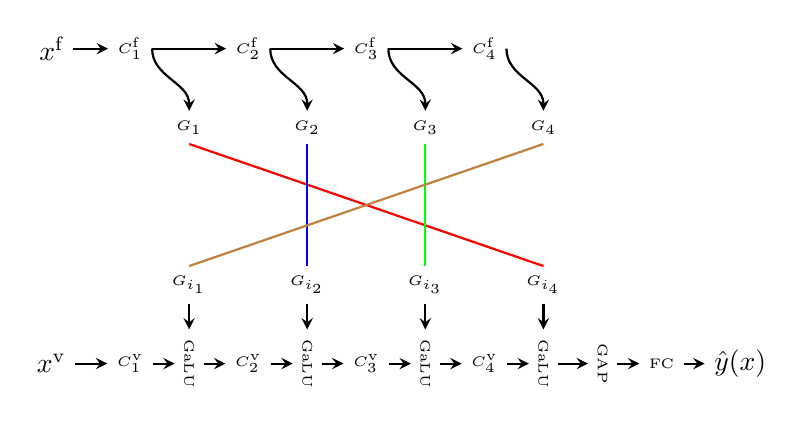
\begin{tikzpicture}
%\node []  (fntext)at (-4.625,-3.5) {CNN-GAP-DLGN};

%\node []  (output) at (7.5,1.5) {$\hat{y}(x)$};


\node [] (dgn1-f-c4) at (-3.5,1.5){\tiny{$C^{\text{f}}_4$}};
\node [] (dgn1-f-c3) at (-5,1.5){\tiny{$C^{\text{f}}_3$}};
\node [] (dgn1-f-c2) at (-6.5,1.5){\tiny{$C^{\text{f}}_2$}};
\node [] (dgn1-f-c1) at (-8,1.5){\tiny{$C^{\text{f}}_1$}};
\node [] (dgn1-input-f) at (-9,1.5){$x^{\text{f}}$};
\draw [-stealth,thick]   (dgn1-f-c3.east) -- (dgn1-f-c4.west);
\draw [-stealth,thick]   (dgn1-f-c2.east) -- (dgn1-f-c3.west);
\draw [-stealth,thick]   (dgn1-f-c1.east) -- (dgn1-f-c2.west);
\draw [-stealth,thick]   (dgn1-input-f.east) -- (dgn1-f-c1.west);



\node []  (dgn1-output) at (-0.25,-2.5) {$\hat{y}(x)$};

\node [] (dgn1-smax) at (-1.25,-2.5){\tiny{FC}};
\draw [-stealth,thick]   (dgn1-smax.east)--(dgn1-output.west);

\node [rotate=-90] (dgn1-gap) at (-2,-2.5){\tiny{GAP}};
\draw [-stealth,thick]   (dgn1-gap.north)--(dgn1-smax.west);


\node [rotate=-90] (dgn1-galu-4) at (-2.75,-2.5){\tiny{GaLU}};
\draw [-stealth,thick]   (dgn1-galu-4.north)--(dgn1-gap.south);

\node [] (dgn1-v-c4) at (-3.5,-2.5){\tiny{$C^{\text{v}}_4$}};
\draw [-stealth,thick]   (dgn1-v-c4.east) -- (dgn1-galu-4.south);


\node [rotate=-90] (dgn1-galu-3) at (-4.25,-2.5){\tiny{GaLU}};
\draw [-stealth,thick]   (dgn1-galu-3.north) -- (dgn1-v-c4.west);

\node [] (dgn1-v-c3) at (-5,-2.5){\tiny{$C^{\text{v}}_3$}};
\draw [-stealth,thick]   (dgn1-v-c3.east) -- (dgn1-galu-3.south);


\node [rotate=-90] (dgn1-galu-2) at (-5.75,-2.5){\tiny{GaLU}};
\draw [-stealth,thick]   (dgn1-galu-2.north) -- (dgn1-v-c3.west);

\node [] (dgn1-v-c2) at (-6.5,-2.5){\tiny{$C^{\text{v}}_2$}};
\draw [-stealth,thick]   (dgn1-v-c2.east) -- (dgn1-galu-2.south);


\node [rotate=-90] (dgn1-galu-1) at (-7.25,-2.5){\tiny{GaLU}};
\draw [-stealth,thick]   (dgn1-galu-1.north) -- (dgn1-v-c2.west);


\node [] (dgn1-v-c1) at (-8,-2.5){\tiny{$C^{\text{v}}_1$}};
\draw [-stealth,thick]   (dgn1-v-c1.east) -- (dgn1-galu-1.south);


\node [] (dgn1-v-input) at (-9,-2.5){$x^{\text{v}}$};

\draw [-stealth,thick]   (dgn1-v-input.east) -- (dgn1-v-c1.west);


\node[] (dgn1-gating-4-up) at (-2.75,0.5){\tiny{$G_{4}$}};
\draw [-stealth,thick]   (dgn1-f-c4.east) to[out=-90,in=90] (dgn1-gating-4-up.north);


\node[] (dgn1-gating-3-up) at (-4.25,0.5){\tiny{$G_{3}$}};
\draw [-stealth,thick]   (dgn1-f-c3.east) to[out=-90,in=90] (dgn1-gating-3-up.north);



\node[] (dgn1-gating-2-up) at (-5.75,0.5){\tiny{$G_{2}$}};
\draw [-stealth,thick]   (dgn1-f-c2.east) to[out=-90,in=90] (dgn1-gating-2-up.north);


\node[] (dgn1-gating-1-up) at (-7.25,0.5){\tiny{$G_{1}$}};
\draw [-stealth,thick]   (dgn1-f-c1.east) to[out=-90,in=90] (dgn1-gating-1-up.north);





\node[] (dgn1-gating-4) at (-2.75,-1.5){\tiny{$G_{i_4}$}};
\draw [-stealth,thick]   (dgn1-gating-4.south) -- (dgn1-galu-4.west);


\node[] (dgn1-gating-3) at (-4.25,-1.5){\tiny{$G_{i_3}$}};
\draw [-stealth,thick]   (dgn1-gating-3.south) -- (dgn1-galu-3.west);



\node[] (dgn1-gating-2) at (-5.75,-1.5){\tiny{$G_{i_2}$}};
\draw [-stealth,thick]   (dgn1-gating-2.south) -- (dgn1-galu-2.west);


\node[] (dgn1-gating-1) at (-7.25,-1.5){\tiny{$G_{i_1}$}};
\draw [-stealth,thick]   (dgn1-gating-1.south) -- (dgn1-galu-1.west);



\draw [-,thick,color=red]   (dgn1-gating-1-up.south) --(dgn1-gating-4.north);

\draw [-,thick,color=blue]   (dgn1-gating-2-up.south) --(dgn1-gating-2.north);

\draw [-,thick,color=green]   (dgn1-gating-3-up.south) --(dgn1-gating-3.north);

\draw [-,thick,color=brown]   (dgn1-gating-4-up.south) --(dgn1-gating-1.north);


%%%%%%%%%%%%%%%%%%%%%%%%%%%%%%%%%%%%%%%%%%%%%%%%%%%%%%%%%%%%%%%%%
	
\end{tikzpicture}


}
\end{minipage}
\caption{Shows the permutations $13-24$ C4GAP-DLGN in Table I of \Cref{fig:c4gap}.}
\label{fig:perm1}
\end{figure}


\begin{figure}
\centering
\begin{minipage}{0.3\columnwidth}
\resizebox{!}{20cm}{
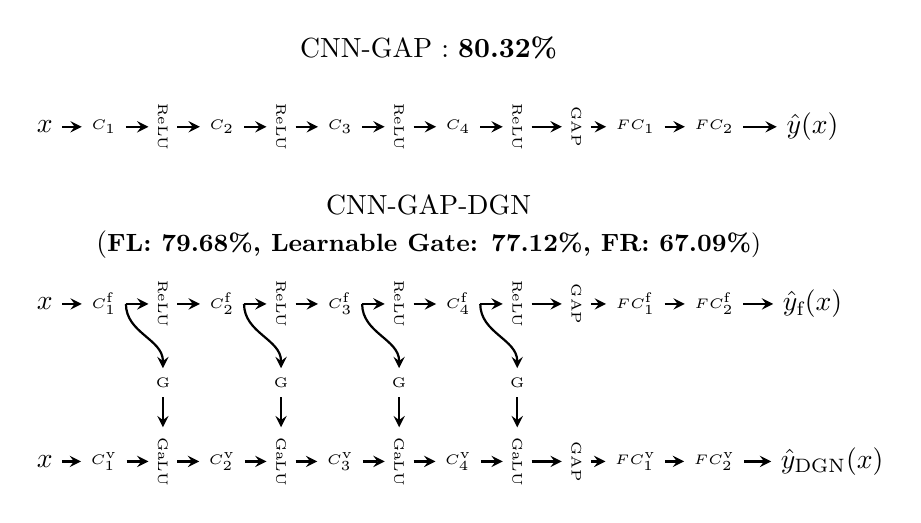
\begin{tikzpicture}
\node []  (dnn-text)at (5.375,2) {CNN-GAP : \textbf{80.32\%}};

\node []  (dnn-output) at (10.25,1) {$\hat{y}(x)$};
\node []  (dnn-fc2) at (9.0,1) {\tiny{$FC_2$}};
\draw [-stealth,thick]   (dnn-fc2.east) -- (dnn-output.west);

\node []  (dnn-fc1) at (8,1) {\tiny{$FC_1$}};
\draw [-stealth,thick]   (dnn-fc1.east) -- (dnn-fc2.west);

\node [rotate=-90]  (dnn-gap) at (7.25,1) {\tiny{GAP}};
\draw [-stealth,thick]   (dnn-gap.north) -- (dnn-fc1.west);

\node [rotate=-90] (dnn-relu-4) at (6.5,1){\tiny{ReLU}};
\node [] (dnn-c4) at (5.75,1){\tiny{$C_4$}};
\draw [-stealth,thick]   (dnn-c4.east) -- (dnn-relu-4.south);
\draw [-stealth,thick]   (dnn-relu-4.north) -- (dnn-gap.south);



\node [rotate=-90] (dnn-relu-3) at (5,1){\tiny{ReLU}};
\node [] (dnn-c3) at (4.25,1){\tiny{$C_3$}};
\draw [-stealth,thick]   (dnn-c3.east) -- (dnn-relu-3.south);
\draw [-stealth,thick]   (dnn-relu-3.north) -- (dnn-c4.west);


\node [rotate=-90] (dnn-relu-2) at (3.5,1){\tiny{ReLU}};
\node [] (dnn-c2) at (2.75,1){\tiny{$C_2$}};
\draw [-stealth,thick]   (dnn-c2.east) -- (dnn-relu-2.south);
\draw [-stealth,thick]   (dnn-relu-2.north) -- (dnn-c3.west);

\node [rotate=-90] (dnn-relu-1) at (2,1){\tiny{ReLU}};
\node [] (dnn-c1) at (1.25,1){\tiny{$C_1$}};
\draw [-stealth,thick]   (dnn-c1.east) -- (dnn-relu-1.south);
\draw [-stealth,thick]   (dnn-relu-1.north) -- (dnn-c2.west);



\node [] (dnn-input) at (0.5,1){$x$};
\draw [-stealth,thick]   (dnn-input.east) -- (dnn-c1.west);


%%%%%%%%%%%%%%%%%%%%%%%%%%%%%%%%%%%%%%%%%%%%%%%%%%%%%%%%%%%%%%%%%
\node []  (fntext)at (5.375,0) {CNN-GAP-DGN};
\node []  (fntext)at (5.375,-.5) {(\small{\textbf{FL: 79.68\%, Learnable Gate: 77.12\%, FR: 67.09\%}})};

%\node []  (output) at (7.5,1.5) {$\hat{y}(x)$};


\node [align=right]  (dgn-f-output) at (10.25,-1.25) {$\hat{y}_{\text{f}}(x)$};
\node []  (dgn-f-fc2) at (9.0,-1.25) {\tiny{$FC^{\text{f}}_2$}};
\draw [-stealth,thick]   (dgn-f-fc2.east) -- (dgn-f-output.west);


\node []  (dgn-f-fc1) at (8,-1.25) {\tiny{$FC^{\text{f}}_1$}};
\draw [-stealth,thick]   (dgn-f-fc1.east) -- (dgn-f-fc2.west);




\node [rotate=-90]  (dgn-f-gap) at (7.25,-1.25) {\tiny{GAP}};
\draw [-stealth,thick]   (dgn-f-gap.north) -- (dgn-f-fc1.west);


\node [rotate=-90] (dgn-relu-4) at (6.5,-1.25){\tiny{ReLU}};
\node [] (dgn-f-c4) at (5.75,-1.25){\tiny{$C^{\text{f}}_4$}};
\draw [-stealth,thick]   (dgn-f-c4.east) -- (dgn-relu-4.south);
\draw [-stealth,thick]   (dgn-relu-4.north) -- (dgn-f-gap.south);


\node [rotate=-90] (dgn-relu-3) at (5,-1.25){\tiny{ReLU}};
\node [] (dgn-f-c3) at (4.25,-1.25){\tiny{$C^{\text{f}}_3$}};
\draw [-stealth,thick]   (dgn-f-c3.east) -- (dgn-relu-3.south);
\draw [-stealth,thick]   (dgn-relu-3.north) -- (dgn-f-c4.west);


\node [rotate=-90] (dgn-relu-2) at (3.5,-1.25){\tiny{ReLU}};
\node [] (dgn-f-c2) at (2.75,-1.25){\tiny{$C^{\text{f}}_2$}};
\draw [-stealth,thick]   (dgn-f-c2.east) -- (dgn-relu-2.south);
\draw [-stealth,thick]   (dgn-relu-2.north) -- (dgn-f-c3.west);


\node [rotate=-90] (dgn-relu-1) at (2,-1.25){\tiny{ReLU}};
\node [] (dgn-f-c1) at (1.25,-1.25){\tiny{$C^{\text{f}}_1$}};
\draw [-stealth,thick]   (dgn-f-c1.east) -- (dgn-relu-1.south);
\draw [-stealth,thick]   (dgn-relu-1.north) -- (dgn-f-c2.west);



\node [] (dgn-f-input) at (0.5,-1.25){$x$};
\draw [-stealth,thick]   (dgn-f-input.east) -- (dgn-f-c1.west);

\node [align=right]  (dgn-output) at (10.5,-3.25) {$\hat{y}_{\text{DGN}}(x)$};

\node [] (dgn-fc2) at (9,-3.25){\tiny{$FC^{\text{v}}_2$}};
\draw [-stealth,thick]   (dgn-fc2.east)--(dgn-output.west);

\node [] (dgn-fc1) at (8,-3.25){\tiny{$FC^{\text{v}}_1$}};
\draw [-stealth,thick]   (dgn-fc1.east)--(dgn-fc2.west);

\node [rotate=-90] (dgn-gap) at (7.25,-3.25){\tiny{GAP}};
\draw [-stealth,thick]   (dgn-gap.north)--(dgn-fc1.west);



\node [rotate=-90] (dgn-galu-4) at (6.5,-3.25){\tiny{GaLU}};
\draw [-stealth,thick]   (dgn-galu-4.north) -- (dgn-gap.south);

\node [] (dgn-v-c4) at (5.75,-3.25){\tiny{$C^{\text{v}}_4$}};
\draw [-stealth,thick]   (dgn-v-c4.east) -- (dgn-galu-4.south);

\node [rotate=-90] (dgn-galu-3) at (5,-3.25){\tiny{GaLU}};
\node [] (dgn-v-c3) at (4.25,-3.25){\tiny{$C^{\text{v}}_3$}};
\draw [-stealth,thick]   (dgn-v-c3.east) -- (dgn-galu-3.south);
\draw [-stealth,thick]   (dgn-galu-3.north) -- (dgn-v-c4.west);



\node [rotate=-90] (dgn-galu-2) at (3.5,-3.25){\tiny{GaLU}};
\node [] (dgn-v-c2) at (2.75,-3.25){\tiny{$C^{\text{v}}_2$}};
\draw [-stealth,thick]   (dgn-v-c2.east) -- (dgn-galu-2.south);
\draw [-stealth,thick]   (dgn-galu-2.north) -- (dgn-v-c3.west);


\node [rotate=-90] (dgn-galu-1) at (2,-3.25){\tiny{GaLU}};
\node [] (dgn-v-c1) at (1.25,-3.25){\tiny{$C^{\text{v}}_1$}};

\draw [-stealth,thick]   (dgn-v-c1.east) -- (dgn-galu-1.south);
\draw [-stealth,thick]   (dgn-galu-1.north) -- (dgn-v-c2.west);




\node [] (dgn-input) at (0.5,-3.25){$x$};
\draw [-stealth,thick]   (dgn-input.east) -- (dgn-v-c1.west);




\node[] (dgn-gating-1) at (2,-2.25){\tiny{G}};
\draw [-stealth,thick]   (dgn-f-c1.east) to[out=-90,in=90] (dgn-gating-1.north);
\draw [-stealth,thick]   (dgn-gating-1.south) -- (dgn-galu-1.west);


\node[] (dgn-gating-2) at (3.5,-2.25){\tiny{G}};
\draw [-stealth,thick]   (dgn-f-c2.east) to[out=-90,in=90] (dgn-gating-2.north);
\draw [-stealth,thick]   (dgn-gating-2.south) -- (dgn-galu-2.west);



\node[] (dgn-gating-3) at (5,-2.25){\tiny{G}};
\draw [-stealth,thick]   (dgn-f-c3.east) to[out=-90,in=90] (dgn-gating-3.north);
\draw [-stealth,thick]   (dgn-gating-3.south) -- (dgn-galu-3.west);


\node[] (dgn-gating-4) at (6.5,-2.25){\tiny{G}};
\draw [-stealth,thick]   (dgn-f-c4.east) to[out=-90,in=90] (dgn-gating-4.north);
\draw [-stealth,thick]   (dgn-gating-4.south) -- (dgn-galu-4.west);

	
\end{tikzpicture}


}
\end{minipage}
\begin{minipage}{0.3\columnwidth}
\resizebox{!}{20cm}{
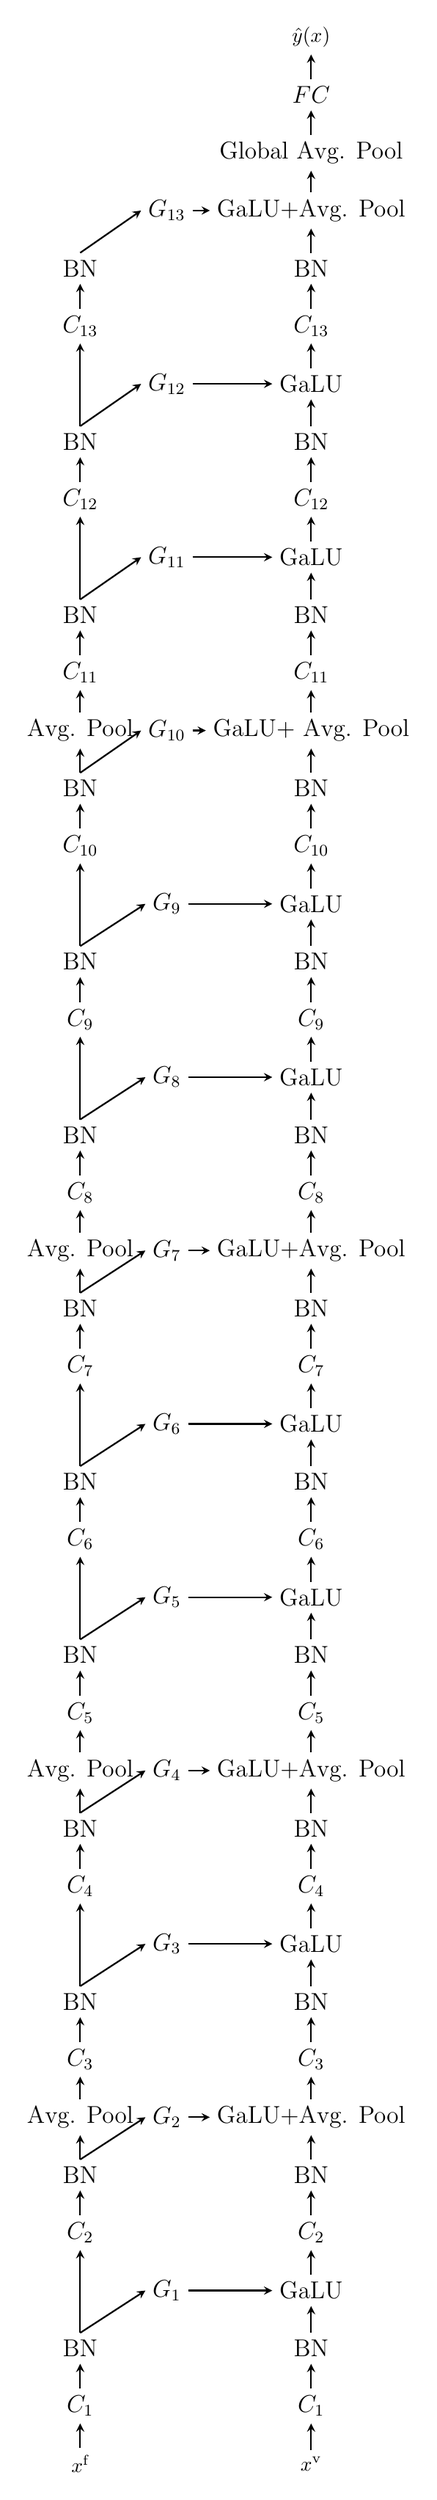
\begin{tikzpicture}


%\node [] (dgn-GaLU-16) at (4,48){\large{GaLU}};
%\draw [-stealth,thick]   (dgn-GaLU-16.north) -- (dgn-c9.south);

%\node [] (dgn-bn-16) at (4,47){\large{BN}};
%\draw [-stealth,thick]   (dgn-bn-16.north) -- (dgn-GaLU-16.south);

%\node [] (dgn-c16) at (4,46){\large{$C_{16}$}};
%\draw [-stealth,thick]   (dgn-c16.north) -- (dgn-bn-16.south);




%\node [] (dgn-GaLU-15) at (4,45){\large{GaLU}};
%\draw [-stealth,thick]   (dgn-GaLU-15.north) -- (dgn-c16.south);

%\node [] (dgn-bn-15) at (4,44){\large{BN}};
%\draw [-stealth,thick]   (dgn-bn-15.north) -- (dgn-GaLU-15.south);

%\node [] (dgn-c15) at (4,43){\large{$C_{15}$}};
%\draw [-stealth,thick]   (dgn-c15.north) -- (dgn-bn-15.south);




\node [] (dgn-GaLU-14) at (4,42){$\hat{y}(x)$};
%\draw [-stealth,thick]   (dgn-GaLU-14.north) -- (dgn-c15.south);

\node [] (dgn-bn-14) at (4,41){\large{$FC$}};
\draw [-stealth,thick]   (dgn-bn-14.north) -- (dgn-GaLU-14.south);

\node [] (dgn-c14) at (4,40){\large{Global Avg. Pool}};
\draw [-stealth,thick]   (dgn-c14.north) -- (dgn-bn-14.south);




\node [] (dgn-GaLU-13) at (4,39){\large{GaLU+Avg. Pool}};
\draw [-stealth,thick]   (dgn-GaLU-13.north) -- (dgn-c14.south);

\node [] (dgn-bn-13) at (4,38){\large{BN}};
\draw [-stealth,thick]   (dgn-bn-13.north) -- (dgn-GaLU-13.south);

\node [] (dgn-c13) at (4,37){\large{$C_{13}$}};
\draw [-stealth,thick]   (dgn-c13.north) -- (dgn-bn-13.south);



\node [] (dgn-GaLU-12) at (4,36){\large{GaLU}};
\draw [-stealth,thick]   (dgn-GaLU-12.north) -- (dgn-c13.south);

\node [] (dgn-bn-12) at (4,35){\large{BN}};
\draw [-stealth,thick]   (dgn-bn-12.north) -- (dgn-GaLU-12.south);

\node [] (dgn-c12) at (4,34){\large{$C_{12}$}};
\draw [-stealth,thick]   (dgn-c12.north) -- (dgn-bn-12.south);



\node [] (dgn-GaLU-11) at (4,33){\large{GaLU}};
\draw [-stealth,thick]   (dgn-GaLU-11.north) -- (dgn-c12.south);

\node [] (dgn-bn-11) at (4,32){\large{BN}};
\draw [-stealth,thick]   (dgn-bn-11.north) -- (dgn-GaLU-11.south);

\node [] (dgn-c11) at (4,31){\large{$C_{11}$}};
\draw [-stealth,thick]   (dgn-c11.north) -- (dgn-bn-11.south);





\node [] (dgn-GaLU-10) at (4,30){\large{GaLU+ Avg. Pool}};
\draw [-stealth,thick]   (dgn-GaLU-10.north) -- (dgn-c11.south);

\node [] (dgn-bn-10) at (4,29){\large{BN}};
\draw [-stealth,thick]   (dgn-bn-10.north) -- (dgn-GaLU-10.south);

\node [] (dgn-c10) at (4,28){\large{$C_{10}$}};
\draw [-stealth,thick]   (dgn-c10.north) -- (dgn-bn-10.south);




\node [] (dgn-GaLU-9) at (4,27){\large{GaLU}};
\draw [-stealth,thick]   (dgn-GaLU-9.north) -- (dgn-c10.south);

\node [] (dgn-bn-9) at (4,26){\large{BN}};
\draw [-stealth,thick]   (dgn-bn-9.north) -- (dgn-GaLU-9.south);

\node [] (dgn-c9) at (4,25){\large{$C_9$}};
\draw [-stealth,thick]   (dgn-c9.north) -- (dgn-bn-9.south);



\node [] (dgn-GaLU-8) at (4,24){\large{GaLU}};
\draw [-stealth,thick]   (dgn-GaLU-8.north) -- (dgn-c9.south);

\node [] (dgn-bn-8) at (4,23){\large{BN}};
\draw [-stealth,thick]   (dgn-bn-8.north) -- (dgn-GaLU-8.south);

\node [] (dgn-c8) at (4,22){\large{$C_8$}};
\draw [-stealth,thick]   (dgn-c8.north) -- (dgn-bn-8.south);




\node [] (dgn-GaLU-7) at (4,21){\large{GaLU+Avg. Pool}};
\draw [-stealth,thick]   (dgn-GaLU-7.north) -- (dgn-c8.south);

\node [] (dgn-bn-7) at (4,20){\large{BN}};
\draw [-stealth,thick]   (dgn-bn-7.north) -- (dgn-GaLU-7.south);

\node [] (dgn-c7) at (4,19){\large{$C_7$}};
\draw [-stealth,thick]   (dgn-c7.north) -- (dgn-bn-7.south);




\node [] (dgn-GaLU-6) at (4,18){\large{GaLU}};
\draw [-stealth,thick]   (dgn-GaLU-6.north) -- (dgn-c7.south);

\node [] (dgn-bn-6) at (4,17){\large{BN}};
\draw [-stealth,thick]   (dgn-bn-6.north) -- (dgn-GaLU-6.south);

\node [] (dgn-c6) at (4,16){\large{$C_6$}};
\draw [-stealth,thick]   (dgn-c6.north) -- (dgn-bn-6.south);




\node [] (dgn-GaLU-5) at (4,15){\large{GaLU}};
\draw [-stealth,thick]   (dgn-GaLU-5.north) -- (dgn-c6.south);

\node [] (dgn-bn-5) at (4,14){\large{BN}};
\draw [-stealth,thick]   (dgn-bn-5.north) -- (dgn-GaLU-5.south);

\node [] (dgn-c5) at (4,13){\large{$C_5$}};
\draw [-stealth,thick]   (dgn-c5.north) -- (dgn-bn-5.south);



\node [] (dgn-GaLU-4) at (4,12){\large{GaLU+Avg. Pool}};
\draw [-stealth,thick]   (dgn-GaLU-4.north) -- (dgn-c5.south);

\node [] (dgn-bn-4) at (4,11){\large{BN}};
\draw [-stealth,thick]   (dgn-bn-4.north) -- (dgn-GaLU-4.south);

\node [] (dgn-c4) at (4,10){\large{$C_4$}};
\draw [-stealth,thick]   (dgn-c4.north) -- (dgn-bn-4.south);



\node [] (dgn-GaLU-3) at (4,9){\large{GaLU}};
\draw [-stealth,thick]   (dgn-GaLU-3.north) -- (dgn-c4.south);

\node [] (dgn-bn-3) at (4,8){\large{BN}};
\draw [-stealth,thick]   (dgn-bn-3.north) -- (dgn-GaLU-3.south);

\node [] (dgn-c3) at (4,7){\large{$C_3$}};
\draw [-stealth,thick]   (dgn-c3.north) -- (dgn-bn-3.south);





\node [] (dgn-GaLU-2) at (4,6){\large{GaLU+Avg. Pool}};
\draw [-stealth,thick]   (dgn-GaLU-2.north) -- (dgn-c3.south);

\node [] (dgn-bn-2) at (4,5){\large{BN}};
\draw [-stealth,thick]   (dgn-bn-2.north) -- (dgn-GaLU-2.south);

\node [] (dgn-c2) at (4,4){\large{$C_2$}};
\draw [-stealth,thick]   (dgn-c2.north) -- (dgn-bn-2.south);




\node [] (dgn-GaLU-1) at (4,3){\large{GaLU}};
\draw [-stealth,thick]   (dgn-GaLU-1.north) -- (dgn-c2.south);

\node [] (dgn-bn-1) at (4,2){\large{BN}};
\draw [-stealth,thick]   (dgn-bn-1.north) -- (dgn-GaLU-1.south);

\node [] (dgn-c1) at (4,1){\large{$C_1$}};
\draw [-stealth,thick]   (dgn-c1.north) -- (dgn-bn-1.south);



\node [] (dgn-input) at (4,0){$x^{\text{v}}$};
\draw [-stealth,thick]   (dgn-input.north) -- (dgn-c1.south);


%%%%%%%%%%%%%%%%%%%%%%%%%%%%%%%%%%%%%%%%%%%%%%%%%%%%%%%%%%%%%%%%%


%\node [] (dnn-relu-16) at (0,48){\large{ReLU}};
%\draw [-stealth,thick]   (dnn-relu-16.north) -- (dnn-c9.south);

%\node [] (dnn-bn-16) at (0,47){\large{BN}};
%\draw [-stealth,thick]   (dnn-bn-16.north) -- (dnn-relu-16.south);

%\node [] (dnn-c16) at (0,46){\large{$C_{16}$}};
%\draw [-stealth,thick]   (dnn-c16.north) -- (dnn-bn-16.south);




%\node [] (dnn-relu-15) at (0,45){\large{ReLU}};
%\draw [-stealth,thick]   (dnn-relu-15.north) -- (dnn-c16.south);

%\node [] (dnn-bn-15) at (0,44){\large{BN}};
%\draw [-stealth,thick]   (dnn-bn-15.north) -- (dnn-relu-15.south);

%\node [] (dnn-c15) at (0,43){\large{$C_{15}$}};
%\draw [-stealth,thick]   (dnn-c15.north) -- (dnn-bn-15.south);




%\node [] (dnn-relu-14) at (0,42){\large{Softmax}};
%\draw [-stealth,thick]   (dnn-relu-14.north) -- (dnn-c15.south);

%\node [] (dnn-bn-14) at (0,41){\large{Fully Connected}};
%\draw [-stealth,thick]   (dnn-bn-14.north) -- (dnn-relu-14.south);

%\node [] (dnn-c14) at (0,40){\large{Global Avg. Pool}};
%\draw [-stealth,thick]   (dnn-c14.north) -- (dnn-bn-14.south);




%\node [] (dnn-relu-13) at (0,39){\large{Avg. Pool}};
%\draw [-stealth,thick]   (dnn-relu-13.north) -- (dnn-c14.south);

\node [] (dnn-bn-13) at (0,38){\large{BN}};
%\draw [-stealth,thick]   (dnn-bn-13.north) -- (dnn-relu-13.south);

\node [] (dnn-gate-13) at (1.5,39){\large{$G_{13}$}};
\draw [-stealth,thick]   (dnn-bn-13.north) -- (dnn-gate-13.west);
\draw [-stealth,thick]   (dnn-gate-13.east) -- (dgn-GaLU-13.west);

\node [] (dnn-c13) at (0,37){\large{$C_{13}$}};
\draw [-stealth,thick]   (dnn-c13.north) -- (dnn-bn-13.south);



%\node [] (dnn-relu-12) at (0,36){\large{ReLU}};
%\draw [-stealth,thick]   (dnn-relu-12.north) -- (dnn-c13.south);

\node [] (dnn-bn-12) at (0,35){\large{BN}};
\draw [-stealth,thick]   (dnn-bn-12.north) -- (dnn-c13.south);

\node [] (dnn-gate-12) at (1.5,36){\large{$G_{12}$}};
\draw [-stealth,thick]   (dnn-bn-12.north) -- (dnn-gate-12.west);
\draw [-stealth,thick]   (dnn-gate-12.east) -- (dgn-GaLU-12.west);

\node [] (dnn-c12) at (0,34){\large{$C_{12}$}};
\draw [-stealth,thick]   (dnn-c12.north) -- (dnn-bn-12.south);



%\node [] (dnn-relu-11) at (0,33){\large{ReLU}};
%\draw [-stealth,thick]   (dnn-relu-11.north) -- (dnn-c12.south);

\node [] (dnn-bn-11) at (0,32){\large{BN}};
\draw [-stealth,thick]   (dnn-bn-11.north) -- (dnn-c12.south);

\node [] (dnn-gate-11) at (1.5,33){\large{$G_{11}$}};
\draw [-stealth,thick]   (dnn-bn-11.north) -- (dnn-gate-11.west);
\draw [-stealth,thick]   (dnn-gate-11.east) -- (dgn-GaLU-11.west);


\node [] (dnn-c11) at (0,31){\large{$C_{11}$}};
\draw [-stealth,thick]   (dnn-c11.north) -- (dnn-bn-11.south);





\node [] (dnn-relu-10) at (0,30){\large{Avg. Pool}};
\draw [-stealth,thick]   (dnn-relu-10.north) -- (dnn-c11.south);

\node [] (dnn-bn-10) at (0,29){\large{BN}};
\draw [-stealth,thick]   (dnn-bn-10.north) -- (dnn-relu-10.south);

\node [] (dnn-gate-10) at (1.5,30){\large{$G_{10}$}};
\draw [-stealth,thick]   (dnn-bn-10.north) -- (dnn-gate-10.west);
\draw [-stealth,thick]   (dnn-gate-10.east) -- (dgn-GaLU-10.west);


\node [] (dnn-c10) at (0,28){\large{$C_{10}$}};
\draw [-stealth,thick]   (dnn-c10.north) -- (dnn-bn-10.south);




%\node [] (dnn-relu-9) at (0,27){\large{ReLU}};
%\draw [-stealth,thick]   (dnn-relu-9.north) -- (dnn-c10.south);

\node [] (dnn-bn-9) at (0,26){\large{BN}};
\draw [-stealth,thick]   (dnn-bn-9.north) -- (dnn-c10.south);

\node [] (dnn-gate-9) at (1.5,27){\large{$G_{9}$}};
\draw [-stealth,thick]   (dnn-bn-9.north) -- (dnn-gate-9.west);
\draw [-stealth,thick]   (dnn-gate-9.east) -- (dgn-GaLU-9.west);

\node [] (dnn-c9) at (0,25){\large{$C_9$}};
\draw [-stealth,thick]   (dnn-c9.north) -- (dnn-bn-9.south);



%\node [] (dnn-relu-8) at (0,24){\large{ReLU}};
%\draw [-stealth,thick]   (dnn-relu-8.north) -- (dnn-c9.south);

\node [] (dnn-bn-8) at (0,23){\large{BN}};
\draw [-stealth,thick]   (dnn-bn-8.north) -- (dnn-c9.south);

\node [] (dnn-gate-8) at (1.5,24){\large{$G_{8}$}};
\draw [-stealth,thick]   (dnn-bn-8.north) -- (dnn-gate-8.west);
\draw [-stealth,thick]   (dnn-gate-8.east) -- (dgn-GaLU-8.west);


\node [] (dnn-c8) at (0,22){\large{$C_8$}};
\draw [-stealth,thick]   (dnn-c8.north) -- (dnn-bn-8.south);




\node [] (dnn-relu-7) at (0,21){\large{Avg. Pool}};
\draw [-stealth,thick]   (dnn-relu-7.north) -- (dnn-c8.south);

\node [] (dnn-bn-7) at (0,20){\large{BN}};
\draw [-stealth,thick]   (dnn-bn-7.north) -- (dnn-relu-7.south);

\node [] (dnn-gate-7) at (1.5,21){\large{$G_{7}$}};
\draw [-stealth,thick]   (dnn-bn-7.north) -- (dnn-gate-7.west);
\draw [-stealth,thick]   (dnn-gate-7.east) -- (dgn-GaLU-7.west);


\node [] (dnn-c7) at (0,19){\large{$C_7$}};
\draw [-stealth,thick]   (dnn-c7.north) -- (dnn-bn-7.south);




%\node [] (dnn-relu-6) at (0,18){\large{ReLU}};
%\draw [-stealth,thick]   (dnn-relu-6.north) -- (dnn-c7.south);

\node [] (dnn-bn-6) at (0,17){\large{BN}};
\draw [-stealth,thick]   (dnn-bn-6.north) -- (dnn-c7.south);

\node [] (dnn-gate-6) at (1.5,18){\large{$G_{6}$}};
\draw [-stealth,thick]   (dnn-bn-6.north) -- (dnn-gate-6.west);
\draw [-stealth,thick]   (dnn-gate-6.east) -- (dgn-GaLU-6.west);



\node [] (dnn-c6) at (0,16){\large{$C_6$}};
\draw [-stealth,thick]   (dnn-c6.north) -- (dnn-bn-6.south);




%\node [] (dnn-relu-5) at (0,15){\large{ReLU}};
%\draw [-stealth,thick]   (dnn-relu-5.north) -- (dnn-c6.south);

\node [] (dnn-bn-5) at (0,14){\large{BN}};
\draw [-stealth,thick]   (dnn-bn-5.north) -- (dnn-c6.south);

\node [] (dnn-gate-5) at (1.5,15){\large{$G_{5}$}};
\draw [-stealth,thick]   (dnn-bn-5.north) -- (dnn-gate-5.west);
\draw [-stealth,thick]   (dnn-gate-5.east) -- (dgn-GaLU-5.west);


\node [] (dnn-c5) at (0,13){\large{$C_5$}};
\draw [-stealth,thick]   (dnn-c5.north) -- (dnn-bn-5.south);



\node [] (dnn-relu-4) at (0,12){\large{Avg. Pool}};
\draw [-stealth,thick]   (dnn-relu-4.north) -- (dnn-c5.south);

\node [] (dnn-bn-4) at (0,11){\large{BN}};
\draw [-stealth,thick]   (dnn-bn-4.north) -- (dnn-relu-4.south);

\node [] (dnn-gate-4) at (1.5,12){\large{$G_{4}$}};
\draw [-stealth,thick]   (dnn-bn-4.north) -- (dnn-gate-4.west);
\draw [-stealth,thick]   (dnn-gate-4.east) -- (dgn-GaLU-4.west);

\node [] (dnn-c4) at (0,10){\large{$C_4$}};
\draw [-stealth,thick]   (dnn-c4.north) -- (dnn-bn-4.south);



%\node [] (dnn-relu-3) at (0,9){\large{ReLU}};
%\draw [-stealth,thick]   (dnn-relu-3.north) -- (dnn-c4.south);

\node [] (dnn-bn-3) at (0,8){\large{BN}};
\draw [-stealth,thick]   (dnn-bn-3.north) -- (dnn-c4.south);

\node [] (dnn-gate-3) at (1.5,9){\large{$G_{3}$}};
\draw [-stealth,thick]   (dnn-bn-3.north) -- (dnn-gate-3.west);
\draw [-stealth,thick]   (dnn-gate-3.east) -- (dgn-GaLU-3.west);

\node [] (dnn-c3) at (0,7){\large{$C_3$}};
\draw [-stealth,thick]   (dnn-c3.north) -- (dnn-bn-3.south);





\node [] (dnn-relu-2) at (0,6){\large{Avg. Pool}};
\draw [-stealth,thick]   (dnn-relu-2.north) -- (dnn-c3.south);

\node [] (dnn-bn-2) at (0,5){\large{BN}};
\draw [-stealth,thick]   (dnn-bn-2.north) -- (dnn-relu-2.south);

\node [] (dnn-gate-2) at (1.5,6){\large{$G_{2}$}};
\draw [-stealth,thick]   (dnn-bn-2.north) -- (dnn-gate-2.west);
\draw [-stealth,thick]   (dnn-gate-2.east) -- (dgn-GaLU-2.west);



\node [] (dnn-c2) at (0,4){\large{$C_2$}};
\draw [-stealth,thick]   (dnn-c2.north) -- (dnn-bn-2.south);





%\draw [-stealth,thick]   (dnn-relu-1.north) -- (dnn-c2.south);

\node [] (dnn-bn-1) at (0,2){\large{BN}};
\draw [-stealth,thick]   (dnn-bn-1.north) -- (dnn-c2.south);

\node [] (dnn-gate-1) at (1.5,3){\large{$G_{1}$}};
\draw [-stealth,thick]   (dnn-bn-1.north) -- (dnn-gate-1.west);
\draw [-stealth,thick]   (dnn-gate-1.east) -- (dgn-GaLU-1.west);


\node [] (dnn-c1) at (0,1){\large{$C_1$}};
\draw [-stealth,thick]   (dnn-c1.north) -- (dnn-bn-1.south);



\node [] (dnn-input) at (0,0){$x^{\text{f}}$};
\draw [-stealth,thick]   (dnn-input.north) -- (dnn-c1.south);

%%%%%%%%%%%%%%%%%%%%%%%%%%%%%%%%%%%%%%%%%%%%%%%%%%%



	
\end{tikzpicture}


}
\end{minipage}
\begin{minipage}{0.3\columnwidth}
\resizebox{!}{20cm}{
\begin{tikzpicture}




%\node [] (dgn-GaLU-16) at (6,48){\large{GaLU}};
%\draw [-stealth,thick]   (dgn-GaLU-16.north) -- (dgn-c9.south);

%\node [] (dgn-bn-16) at (6,47){\large{BN}};
%\draw [-stealth,thick]   (dgn-bn-16.north) -- (dgn-GaLU-16.south);

%\node [] (dgn-c16) at (6,46){\large{$C_{16}$}};
%\draw [-stealth,thick]   (dgn-c16.north) -- (dgn-bn-16.south);




%\node [] (dgn-GaLU-15) at (6,45){\large{GaLU}};
%\draw [-stealth,thick]   (dgn-GaLU-15.north) -- (dgn-c16.south);

%\node [] (dgn-bn-15) at (6,44){\large{BN}};
%\draw [-stealth,thick]   (dgn-bn-15.north) -- (dgn-GaLU-15.south);

%\node [] (dgn-c15) at (6,43){\large{$C_{15}$}};
%\draw [-stealth,thick]   (dgn-c15.north) -- (dgn-bn-15.south);




\node [] (dgn-GaLU-14) at (6,42){$\hat{y}(x)$};
%\draw [-stealth,thick]   (dgn-GaLU-14.north) -- (dgn-c15.south);

\node [] (dgn-bn-14) at (6,41){\large{$FC$}};
\draw [-stealth,thick]   (dgn-bn-14.north) -- (dgn-GaLU-14.south);

\node [] (dgn-c14) at (6,40){\large{Global Avg. Pool}};
\draw [-stealth,thick]   (dgn-c14.north) -- (dgn-bn-14.south);




\node [] (dgn-GaLU-13) at (6,39){\large{GaLU+Avg. Pool}};
\draw [-stealth,thick]   (dgn-GaLU-13.north) -- (dgn-c14.south);

\node [] (dgn-bn-13) at (6,38){\large{BN}};
\draw [-stealth,thick]   (dgn-bn-13.north) -- (dgn-GaLU-13.south);

\node [] (dgn-c13) at (6,37){\large{$C_{13}$}};
\draw [-stealth,thick]   (dgn-c13.north) -- (dgn-bn-13.south);



\node [] (dgn-GaLU-12) at (6,36){\large{GaLU}};
\draw [-stealth,thick]   (dgn-GaLU-12.north) -- (dgn-c13.south);

\node [] (dgn-bn-12) at (6,35){\large{BN}};
\draw [-stealth,thick]   (dgn-bn-12.north) -- (dgn-GaLU-12.south);

\node [] (dgn-c12) at (6,34){\large{$C_{12}$}};
\draw [-stealth,thick]   (dgn-c12.north) -- (dgn-bn-12.south);



\node [] (dgn-GaLU-11) at (6,33){\large{GaLU}};
\draw [-stealth,thick]   (dgn-GaLU-11.north) -- (dgn-c12.south);

\node [] (dgn-bn-11) at (6,32){\large{BN}};
\draw [-stealth,thick]   (dgn-bn-11.north) -- (dgn-GaLU-11.south);

\node [] (dgn-c11) at (6,31){\large{$C_{11}$}};
\draw [-stealth,thick]   (dgn-c11.north) -- (dgn-bn-11.south);





\node [] (dgn-GaLU-10) at (6,30){\large{GaLU+ Avg. Pool}};
\draw [-stealth,thick]   (dgn-GaLU-10.north) -- (dgn-c11.south);

\node [] (dgn-bn-10) at (6,29){\large{BN}};
\draw [-stealth,thick]   (dgn-bn-10.north) -- (dgn-GaLU-10.south);

\node [] (dgn-c10) at (6,28){\large{$C_{10}$}};
\draw [-stealth,thick]   (dgn-c10.north) -- (dgn-bn-10.south);




\node [] (dgn-GaLU-9) at (6,27){\large{GaLU}};
\draw [-stealth,thick]   (dgn-GaLU-9.north) -- (dgn-c10.south);

\node [] (dgn-bn-9) at (6,26){\large{BN}};
\draw [-stealth,thick]   (dgn-bn-9.north) -- (dgn-GaLU-9.south);

\node [] (dgn-c9) at (6,25){\large{$C_9$}};
\draw [-stealth,thick]   (dgn-c9.north) -- (dgn-bn-9.south);



\node [] (dgn-GaLU-8) at (6,24){\large{GaLU}};
\draw [-stealth,thick]   (dgn-GaLU-8.north) -- (dgn-c9.south);

\node [] (dgn-bn-8) at (6,23){\large{BN}};
\draw [-stealth,thick]   (dgn-bn-8.north) -- (dgn-GaLU-8.south);

\node [] (dgn-c8) at (6,22){\large{$C_8$}};
\draw [-stealth,thick]   (dgn-c8.north) -- (dgn-bn-8.south);




\node [] (dgn-GaLU-7) at (6,21){\large{GaLU+Avg. Pool}};
\draw [-stealth,thick]   (dgn-GaLU-7.north) -- (dgn-c8.south);

\node [] (dgn-bn-7) at (6,20){\large{BN}};
\draw [-stealth,thick]   (dgn-bn-7.north) -- (dgn-GaLU-7.south);

\node [] (dgn-c7) at (6,19){\large{$C_7$}};
\draw [-stealth,thick]   (dgn-c7.north) -- (dgn-bn-7.south);




\node [] (dgn-GaLU-6) at (6,18){\large{GaLU}};
\draw [-stealth,thick]   (dgn-GaLU-6.north) -- (dgn-c7.south);

\node [] (dgn-bn-6) at (6,17){\large{BN}};
\draw [-stealth,thick]   (dgn-bn-6.north) -- (dgn-GaLU-6.south);

\node [] (dgn-c6) at (6,16){\large{$C_6$}};
\draw [-stealth,thick]   (dgn-c6.north) -- (dgn-bn-6.south);




\node [] (dgn-GaLU-5) at (6,15){\large{GaLU}};
\draw [-stealth,thick]   (dgn-GaLU-5.north) -- (dgn-c6.south);

\node [] (dgn-bn-5) at (6,14){\large{BN}};
\draw [-stealth,thick]   (dgn-bn-5.north) -- (dgn-GaLU-5.south);

\node [] (dgn-c5) at (6,13){\large{$C_5$}};
\draw [-stealth,thick]   (dgn-c5.north) -- (dgn-bn-5.south);



\node [] (dgn-GaLU-4) at (6,12){\large{GaLU+Avg. Pool}};
\draw [-stealth,thick]   (dgn-GaLU-4.north) -- (dgn-c5.south);

\node [] (dgn-bn-4) at (6,11){\large{BN}};
\draw [-stealth,thick]   (dgn-bn-4.north) -- (dgn-GaLU-4.south);

\node [] (dgn-c4) at (6,10){\large{$C_4$}};
\draw [-stealth,thick]   (dgn-c4.north) -- (dgn-bn-4.south);



\node [] (dgn-GaLU-3) at (6,9){\large{GaLU}};
\draw [-stealth,thick]   (dgn-GaLU-3.north) -- (dgn-c4.south);

\node [] (dgn-bn-3) at (6,8){\large{BN}};
\draw [-stealth,thick]   (dgn-bn-3.north) -- (dgn-GaLU-3.south);

\node [] (dgn-c3) at (6,7){\large{$C_3$}};
\draw [-stealth,thick]   (dgn-c3.north) -- (dgn-bn-3.south);





\node [] (dgn-GaLU-2) at (6,6){\large{GaLU+Avg. Pool}};
\draw [-stealth,thick]   (dgn-GaLU-2.north) -- (dgn-c3.south);

\node [] (dgn-bn-2) at (6,5){\large{BN}};
\draw [-stealth,thick]   (dgn-bn-2.north) -- (dgn-GaLU-2.south);

\node [] (dgn-c2) at (6,4){\large{$C_2$}};
\draw [-stealth,thick]   (dgn-c2.north) -- (dgn-bn-2.south);




\node [] (dgn-GaLU-1) at (6,3){\large{GaLU}};
\draw [-stealth,thick]   (dgn-GaLU-1.north) -- (dgn-c2.south);

\node [] (dgn-bn-1) at (6,2){\large{BN}};
\draw [-stealth,thick]   (dgn-bn-1.north) -- (dgn-GaLU-1.south);

\node [] (dgn-c1) at (6,1){\large{$C_1$}};
\draw [-stealth,thick]   (dgn-c1.north) -- (dgn-bn-1.south);



\node [] (dgn-input) at (6,0){$\mathbf{1}$};
\draw [-stealth,thick]   (dgn-input.north) -- (dgn-c1.south);


%%%%%%%%%%%%%%%%%%%%%%%%%%%%%%%%%%%%%%%%%%%%%%%%%%%%%%%%%%%%%%%%%


%\node [] (dnnsig-relu-16) at (2,48){\large{ReLU}};
%\draw [-stealth,thick]   (dnnsig-relu-16.north) -- (dnnsig-c9.south);

%\node [] (dnnsig-bn-16) at (2,47){\large{BN}};
%\draw [-stealth,thick]   (dnnsig-bn-16.north) -- (dnnsig-relu-16.south);

%\node [] (dnnsig-c16) at (2,46){\large{$C_{16}$}};
%\draw [-stealth,thick]   (dnnsig-c16.north) -- (dnnsig-bn-16.south);




%\node [] (dnnsig-relu-15) at (2,45){\large{ReLU}};
%\draw [-stealth,thick]   (dnnsig-relu-15.north) -- (dnnsig-c16.south);

%\node [] (dnnsig-bn-15) at (2,44){\large{BN}};
%\draw [-stealth,thick]   (dnnsig-bn-15.north) -- (dnnsig-relu-15.south);

%\node [] (dnnsig-c15) at (2,43){\large{$C_{15}$}};
%\draw [-stealth,thick]   (dnnsig-c15.north) -- (dnnsig-bn-15.south);




%\node [] (dnnsig-relu-14) at (2,42){\large{Softmax}};
%\draw [-stealth,thick]   (dnnsig-relu-14.north) -- (dnnsig-c15.south);

%\node [] (dnnsig-bn-14) at (2,41){\large{Fully Connected}};
%\draw [-stealth,thick]   (dnnsig-bn-14.north) -- (dnnsig-relu-14.south);

%\node [] (dnnsig-c14) at (2,40){\large{Global Avg. Pool}};
%\draw [-stealth,thick]   (dnnsig-c14.north) -- (dnnsig-bn-14.south);




%\node [] (dnnsig-relu-13) at (2,39){\large{Avg. Pool}};
%\draw [-stealth,thick]   (dnnsig-relu-13.north) -- (dnnsig-c14.south);

\node [] (dnnsig-bn-13) at (2,38){\large{BN}};
%\draw [-stealth,thick]   (dnnsig-bn-13.north) -- (dnnsig-relu-13.south);

\node [] (dnnsig-gate-13) at (3.5,39){\large{G}};
\draw [-stealth,thick]   (dnnsig-bn-13.north) -- (dnnsig-gate-13.west);
\draw [-stealth,thick]   (dnnsig-gate-13.east) -- (dgn-GaLU-13.west);

\node [] (dnnsig-c13) at (2,37){\large{$C_{13}$}};
\draw [-stealth,thick]   (dnnsig-c13.north) -- (dnnsig-bn-13.south);



%\node [] (dnnsig-relu-12) at (2,36){\large{ReLU}};
%\draw [-stealth,thick]   (dnnsig-relu-12.north) -- (dnnsig-c13.south);

\node [] (dnnsig-bn-12) at (2,35){\large{BN}};
%\draw [-stealth,thick]   (dnnsig-bn-12.north) -- (dnnsig-c13.south);

\node [] (dnnsig-gate-12) at (3.5,36){\large{G}};
\draw [-stealth,thick]   (dnnsig-bn-12.north) -- (dnnsig-gate-12.west);
\draw [-stealth,thick]   (dnnsig-gate-12.east) -- (dgn-GaLU-12.west);

\node [] (dnnsig-c12) at (2,34){\large{$C_{12}$}};
\draw [-stealth,thick]   (dnnsig-c12.north) -- (dnnsig-bn-12.south);



%\node [] (dnnsig-relu-11) at (2,33){\large{ReLU}};
%\draw [-stealth,thick]   (dnnsig-relu-11.north) -- (dnnsig-c12.south);

\node [] (dnnsig-bn-11) at (2,32){\large{BN}};
%\draw [-stealth,thick]   (dnnsig-bn-11.north) -- (dnnsig-c12.south);

\node [] (dnnsig-gate-11) at (3.5,33){\large{G}};
\draw [-stealth,thick]   (dnnsig-bn-11.north) -- (dnnsig-gate-11.west);
\draw [-stealth,thick]   (dnnsig-gate-11.east) -- (dgn-GaLU-11.west);


\node [] (dnnsig-c11) at (2,31){\large{$C_{11}$}};
\draw [-stealth,thick]   (dnnsig-c11.north) -- (dnnsig-bn-11.south);





%\node [] (dnnsig-relu-10) at (2,30){\large{Avg. Pool}};
%\draw [-stealth,thick]   (dnnsig-relu-10.north) -- (dnnsig-c11.south);

\node [] (dnnsig-bn-10) at (2,29){\large{BN}};
%\draw [-stealth,thick]   (dnnsig-bn-10.north) -- (dnnsig-relu-10.south);

\node [] (dnnsig-gate-10) at (3.5,30){\large{G}};
\draw [-stealth,thick]   (dnnsig-bn-10.north) -- (dnnsig-gate-10.west);
\draw [-stealth,thick]   (dnnsig-gate-10.east) -- (dgn-GaLU-10.west);


\node [] (dnnsig-c10) at (2,28){\large{$C_{10}$}};
\draw [-stealth,thick]   (dnnsig-c10.north) -- (dnnsig-bn-10.south);




%\node [] (dnnsig-relu-9) at (2,27){\large{ReLU}};
%\draw [-stealth,thick]   (dnnsig-relu-9.north) -- (dnnsig-c10.south);

\node [] (dnnsig-bn-9) at (2,26){\large{BN}};
%\draw [-stealth,thick]   (dnnsig-bn-9.north) -- (dnnsig-c10.south);

\node [] (dnnsig-gate-9) at (3.5,27){\large{G}};
\draw [-stealth,thick]   (dnnsig-bn-9.north) -- (dnnsig-gate-9.west);
\draw [-stealth,thick]   (dnnsig-gate-9.east) -- (dgn-GaLU-9.west);

\node [] (dnnsig-c9) at (2,25){\large{$C_9$}};
\draw [-stealth,thick]   (dnnsig-c9.north) -- (dnnsig-bn-9.south);



%\node [] (dnnsig-relu-8) at (2,24){\large{ReLU}};
%\draw [-stealth,thick]   (dnnsig-relu-8.north) -- (dnnsig-c9.south);

\node [] (dnnsig-bn-8) at (2,23){\large{BN}};
%\draw [-stealth,thick]   (dnnsig-bn-8.north) -- (dnnsig-c9.south);

\node [] (dnnsig-gate-8) at (3.5,24){\large{G}};
\draw [-stealth,thick]   (dnnsig-bn-8.north) -- (dnnsig-gate-8.west);
\draw [-stealth,thick]   (dnnsig-gate-8.east) -- (dgn-GaLU-8.west);


\node [] (dnnsig-c8) at (2,22){\large{$C_8$}};
\draw [-stealth,thick]   (dnnsig-c8.north) -- (dnnsig-bn-8.south);




%\node [] (dnnsig-relu-7) at (2,21){\large{Avg. Pool}};
%\draw [-stealth,thick]   (dnnsig-relu-7.north) -- (dnnsig-c8.south);

\node [] (dnnsig-bn-7) at (2,20){\large{BN}};
%\draw [-stealth,thick]   (dnnsig-bn-7.north) -- (dnnsig-relu-7.south);

\node [] (dnnsig-gate-7) at (3.5,21){\large{G}};
\draw [-stealth,thick]   (dnnsig-bn-7.north) -- (dnnsig-gate-7.west);
\draw [-stealth,thick]   (dnnsig-gate-7.east) -- (dgn-GaLU-7.west);


\node [] (dnnsig-c7) at (2,19){\large{$C_7$}};
\draw [-stealth,thick]   (dnnsig-c7.north) -- (dnnsig-bn-7.south);




%\node [] (dnnsig-relu-6) at (2,18){\large{ReLU}};
%\draw [-stealth,thick]   (dnnsig-relu-6.north) -- (dnnsig-c7.south);

\node [] (dnnsig-bn-6) at (2,17){\large{BN}};
%\draw [-stealth,thick]   (dnnsig-bn-6.north) -- (dnnsig-c7.south);

\node [] (dnnsig-gate-6) at (3.5,18){\large{G}};
\draw [-stealth,thick]   (dnnsig-bn-6.north) -- (dnnsig-gate-6.west);
\draw [-stealth,thick]   (dnnsig-gate-6.east) -- (dgn-GaLU-6.west);



\node [] (dnnsig-c6) at (2,16){\large{$C_6$}};
\draw [-stealth,thick]   (dnnsig-c6.north) -- (dnnsig-bn-6.south);




%\node [] (dnnsig-relu-5) at (2,15){\large{ReLU}};
%\draw [-stealth,thick]   (dnnsig-relu-5.north) -- (dnnsig-c6.south);

\node [] (dnnsig-bn-5) at (2,14){\large{BN}};
%\draw [-stealth,thick]   (dnnsig-bn-5.north) -- (dnnsig-c6.south);

\node [] (dnnsig-gate-5) at (3.5,15){\large{G}};
\draw [-stealth,thick]   (dnnsig-bn-5.north) -- (dnnsig-gate-5.west);
\draw [-stealth,thick]   (dnnsig-gate-5.east) -- (dgn-GaLU-5.west);


\node [] (dnnsig-c5) at (2,13){\large{$C_5$}};
\draw [-stealth,thick]   (dnnsig-c5.north) -- (dnnsig-bn-5.south);



%\node [] (dnnsig-relu-4) at (2,12){\large{Avg. Pool}};
%\draw [-stealth,thick]   (dnnsig-relu-4.north) -- (dnnsig-c5.south);

\node [] (dnnsig-bn-4) at (2,11){\large{BN}};
%\draw [-stealth,thick]   (dnnsig-bn-4.north) -- (dnnsig-relu-4.south);

\node [] (dnnsig-gate-4) at (3.5,12){\large{G}};
\draw [-stealth,thick]   (dnnsig-bn-4.north) -- (dnnsig-gate-4.west);
\draw [-stealth,thick]   (dnnsig-gate-4.east) -- (dgn-GaLU-4.west);

\node [] (dnnsig-c4) at (2,10){\large{$C_4$}};
\draw [-stealth,thick]   (dnnsig-c4.north) -- (dnnsig-bn-4.south);



%\node [] (dnnsig-relu-3) at (2,9){\large{ReLU}};
%\draw [-stealth,thick]   (dnnsig-relu-3.north) -- (dnnsig-c4.south);

\node [] (dnnsig-bn-3) at (2,8){\large{BN}};
%\draw [-stealth,thick]   (dnnsig-bn-3.north) -- (dnnsig-c4.south);

\node [] (dnnsig-gate-3) at (3.5,9){\large{G}};
\draw [-stealth,thick]   (dnnsig-bn-3.north) -- (dnnsig-gate-3.west);
\draw [-stealth,thick]   (dnnsig-gate-3.east) -- (dgn-GaLU-3.west);

\node [] (dnnsig-c3) at (2,7){\large{$C_3$}};
\draw [-stealth,thick]   (dnnsig-c3.north) -- (dnnsig-bn-3.south);





%\node [] (dnnsig-relu-2) at (2,6){\large{Avg. Pool}};
%\draw [-stealth,thick]   (dnnsig-relu-2.north) -- (dnnsig-c3.south);

\node [] (dnnsig-bn-2) at (2,5){\large{BN}};
%\draw [-stealth,thick]   (dnnsig-bn-2.north) -- (dnnsig-relu-2.south);

\node [] (dnnsig-gate-2) at (3.5,6){\large{G}};
\draw [-stealth,thick]   (dnnsig-bn-2.north) -- (dnnsig-gate-2.west);
\draw [-stealth,thick]   (dnnsig-gate-2.east) -- (dgn-GaLU-2.west);



\node [] (dnnsig-c2) at (2,4){\large{$C_2$}};
\draw [-stealth,thick]   (dnnsig-c2.north) -- (dnnsig-bn-2.south);





%\draw [-stealth,thick]   (dnnsig-relu-1.north) -- (dnnsig-c2.south);

\node [] (dnnsig-bn-1) at (2,2){\large{BN}};
%\draw [-stealth,thick]   (dnnsig-bn-1.north) -- (dnnsig-c2.south);

\node [] (dnnsig-gate-1) at (3.5,3){\large{G}};
\draw [-stealth,thick]   (dnnsig-bn-1.north) -- (dnnsig-gate-1.west);
\draw [-stealth,thick]   (dnnsig-gate-1.east) -- (dgn-GaLU-1.west);


\node [] (dnnsig-c1) at (2,1){\large{$C_1$}};
\draw [-stealth,thick]   (dnnsig-c1.north) -- (dnnsig-bn-1.south);



%\node [] (dnnsig-input) at (2,0){$x$};


\draw [-stealth,thick]   (dnn-c1.center) -- (dnnsig-c1.west);
\draw [-stealth,thick]   (dnn-c2.center) -- (dnnsig-c2.west);
\draw [-stealth,thick]   (dnn-c3.center) -- (dnnsig-c3.west);
\draw [-stealth,thick]   (dnn-c4.center) -- (dnnsig-c4.west);
\draw [-stealth,thick]   (dnn-c5.center) -- (dnnsig-c5.west);
\draw [-stealth,thick]   (dnn-c6.center) -- (dnnsig-c6.west);
\draw [-stealth,thick]   (dnn-c7.center) -- (dnnsig-c7.west);
\draw [-stealth,thick]   (dnn-c8.center) -- (dnnsig-c8.west);
\draw [-stealth,thick]   (dnn-c9.center) -- (dnnsig-c9.west);
\draw [-stealth,thick]   (dnn-c10.center) -- (dnnsig-c10.west);
\draw [-stealth,thick]   (dnn-c11.center) -- (dnnsig-c11.west);
\draw [-stealth,thick]   (dnn-c12.center) -- (dnnsig-c12.west);
\draw [-stealth,thick]   (dnn-c13.center) -- (dnnsig-c13.west);





%\draw [-stealth,thick]   (dnnsig-input.north) -- (dnnsig-c1.south);

%%%%%%%%%%%%%%%%%%%%%%%%%%%%%%%%%%%%%%%%%%%%%%%%%%%

%%%%%%%%%%%%%%%%%%%%%%%%%%%%%%%%%%%%%%%%%%%%%%%%%%%%%%%%%%%%%%%%%



%\node [] (dnn-relu-16) at (0,48){\large{ReLU}};
%\draw [-stealth,thick]   (dnn-relu-16.north) -- (dnn-c9.south);

%\node [] (dnn-bn-16) at (0,47){\large{BN}};
%\draw [-stealth,thick]   (dnn-bn-16.north) -- (dnn-relu-16.south);

%\node [] (dnn-c16) at (0,46){\large{$C_{16}$}};
%\draw [-stealth,thick]   (dnn-c16.north) -- (dnn-bn-16.south);




%\node [] (dnn-relu-15) at (0,45){\large{ReLU}};
%\draw [-stealth,thick]   (dnn-relu-15.north) -- (dnn-c16.south);

%\node [] (dnn-bn-15) at (0,44){\large{BN}};
%\draw [-stealth,thick]   (dnn-bn-15.north) -- (dnn-relu-15.south);

%\node [] (dnn-c15) at (0,43){\large{$C_{15}$}};
%\draw [-stealth,thick]   (dnn-c15.north) -- (dnn-bn-15.south);




%\node [] (dnn-relu-14) at (0,42){\large{Softmax}};
%\draw [-stealth,thick]   (dnn-relu-14.north) -- (dnn-c15.south);

%\node [] (dnn-bn-14) at (0,41){\large{Fully Connected}};
%\draw [-stealth,thick]   (dnn-bn-14.north) -- (dnn-relu-14.south);

%\node [] (dnn-c14) at (0,40){\large{Global Avg. Pool}};
%\draw [-stealth,thick]   (dnn-c14.north) -- (dnn-bn-14.south);




%\node [] (dnn-relu-13) at (0,39){\large{Avg. Pool}};
%\draw [-stealth,thick]   (dnn-relu-13.north) -- (dnn-c14.south);

\node [] (dnn-bn-13) at (0,38){};
%\draw [-stealth,thick]   (dnn-bn-13.north) -- (dnn-relu-13.south);


\node [] (dnn-c13) at (0,37){};
%\draw [-stealth,thick]   (dnn-c13.north) -- (dnn-bn-13.south);



%\node [] (dnn-relu-12) at (0,36){\large{ReLU}};
%\draw [-stealth,thick]   (dnn-relu-12.north) -- (dnn-c13.south);

\node [] (dnn-bn-12) at (0,35){};
%\draw [-stealth,thick]   (dnn-bn-12.north) -- (dnn-c13.south);


\node [] (dnn-c12) at (0,34){};
%\draw [-stealth,thick]   (dnn-c12.north) -- (dnn-bn-12.south);



%\node [] (dnn-relu-11) at (0,33){\large{ReLU}};
%\draw [-stealth,thick]   (dnn-relu-11.north) -- (dnn-c12.south);

\node [] (dnn-bn-11) at (0,32){};
%\draw [-stealth,thick]   (dnn-bn-11.north) -- (dnn-c12.south);



\node [] (dnn-c11) at (0,31){};
%\draw [-stealth,thick]   (dnn-c11.north) -- (dnn-bn-11.south);





\node [] (dnn-relu-10) at (0,30){\large{Avg. Pool}};
\draw [-,thick]   (dnn-relu-10.north) -- (dnn-c13.center);

\node [] (dnn-bn-10) at (0,29){};
%\draw [-stealth,thick]   (dnn-bn-10.north) -- (dnn-relu-10.south);



\node [] (dnn-c10) at (0,28){};
%\draw [-stealth,thick]   (dnn-c10.north) -- (dnn-bn-10.south);




%\node [] (dnn-relu-9) at (0,27){\large{ReLU}};
%\draw [-stealth,thick]   (dnn-relu-9.north) -- (dnn-c10.south);

\node [] (dnn-bn-9) at (0,26){};
%\draw [-stealth,thick]   (dnn-bn-9.north) -- (dnn-c10.south);


\node [] (dnn-c9) at (0,25){};
%\draw [-stealth,thick]   (dnn-c9.north) -- (dnn-bn-9.south);



%\node [] (dnn-relu-8) at (0,24){\large{ReLU}};
%\draw [-stealth,thick]   (dnn-relu-8.north) -- (dnn-c9.south);

\node [] (dnn-bn-8) at (0,23){};
%\draw [-stealth,thick]   (dnn-bn-8.north) -- (dnn-c9.south);



\node [] (dnn-c8) at (0,22){};
%\draw [-stealth,thick]   (dnn-c8.north) -- (dnn-bn-8.south);




\node [] (dnn-relu-7) at (0,21){\large{Avg. Pool}};
\draw [-stealth,thick]   (dnn-relu-7.north) -- (dnn-relu-10.south);

\node [] (dnn-bn-7) at (0,20){};
%\draw [-stealth,thick]   (dnn-bn-7.north) -- (dnn-relu-7.south);



\node [] (dnn-c7) at (0,19){};
%\draw [-stealth,thick]   (dnn-c7.north) -- (dnn-bn-7.south);




%\node [] (dnn-relu-6) at (0,18){\large{ReLU}};
%\draw [-stealth,thick]   (dnn-relu-6.north) -- (dnn-c7.south);

\node [] (dnn-bn-6) at (0,17){};
%\draw [-stealth,thick]   (dnn-bn-6.north) -- (dnn-c7.south);




\node [] (dnn-c6) at (0,16){};
%\draw [-stealth,thick]   (dnn-c6.north) -- (dnn-bn-6.south);




%\node [] (dnn-relu-5) at (0,15){\large{ReLU}};
%\draw [-stealth,thick]   (dnn-relu-5.north) -- (dnn-c6.south);

\node [] (dnn-bn-5) at (0,14){};
%\draw [-stealth,thick]   (dnn-bn-5.north) -- (dnn-c6.south);



\node [] (dnn-c5) at (0,13){};
%\draw [-stealth,thick]   (dnn-c5.north) -- (dnn-bn-5.south);



\node [] (dnn-relu-4) at (0,12){\large{Avg. Pool}};
\draw [-stealth,thick]   (dnn-relu-4.north) -- (dnn-relu-7.south);

\node [] (dnn-bn-4) at (0,11){};
%\draw [-stealth,thick]   (dnn-bn-4.north) -- (dnn-relu-4.south);


\node [] (dnn-c4) at (0,10){};
%\draw [-stealth,thick]   (dnn-c4.north) -- (dnn-bn-4.south);



%\node [] (dnn-relu-3) at (0,9){\large{ReLU}};
%\draw [-stealth,thick]   (dnn-relu-3.north) -- (dnn-c4.south);

\node [] (dnn-bn-3) at (0,8){};
%\draw [-stealth,thick]   (dnn-bn-3.north) -- (dnn-c4.south);


\node [] (dnn-c3) at (0,7){};
%\draw [-stealth,thick]   (dnn-c3.north) -- (dnn-bn-3.south);





\node [] (dnn-relu-2) at (0,6){\large{Avg. Pool}};
\draw [-stealth,thick]   (dnn-relu-2.north) -- (dnn-relu-4.south);

\node [] (dnn-bn-2) at (0,5){};
%\draw [-stealth,thick]   (dnn-bn-2.north) -- (dnn-relu-2.south);




\node [] (dnn-c2) at (0,4){};
%\draw [-stealth,thick]   (dnn-c2.north) -- (dnn-bn-2.south);





%\draw [-stealth,thick]   (dnn-relu-1.north) -- (dnn-c2.south);

\node [] (dnn-bn-1) at (0,2){};
%\draw [-stealth,thick]   (dnn-bn-1.north) -- (dnn-c2.south);



\node [] (dnn-c1) at (0,1){};
%\draw [-stealth,thick]   (dnn-c1.north) -- (dnn-bn-1.south);



\node [] (dnn-input) at (0,0){$x$};
\draw [-stealth,thick]   (dnn-input.north) -- (dnn-relu-2.south);




%%%%%%%%%%%%%%%%%%%%%%%%%%%%%%%%%%%%%%%%%%%%%%%%%%%



	








	
\end{tikzpicture}


}
\end{minipage}
\caption{Shows VGG-16 (left), VGG-16-DLGN (middle), VGG-16-DLGN-SF(right).}
\label{fig:vggnets}
\end{figure}


You may include other additional sections here.
%\end{comment}
\end{document}

